\documentclass[final]{scrreprt} % setting of the document class; only the KOMA-Script classes are allowed here as this document uses many of those features

%%%%%%%%%%%%%%%%%%%%%%%%%%%%%%%%%%%%%%%%%%%%%%%
%%%%%%%%%%%%%%%%%%%%%%%%%%%%%%%%%%%%%%%%%%%%%%%
%%%%%%%%%%%%%%%%%%%%%%%%%%%%%%%%%%%%%%%%%%%%%%%
% Allows to align the headings of the numbered structure levels to the text using 
% \settoggle{alignheadings}{true} OR \toggletrue{alignheadings}:
%%%%%%%%%%%%%%%%%%%%%%%%%%%%%%%%%%%%%%%%%%%%%%% begindefinition
\usepackage{etoolbox}

\newtoggle{alignheadings}

\renewcommand*{\chapterformat}{%
    \iftoggle{alignheadings}{%
        \IfChapterUsesPrefixLine{%
            \chapapp~\thechapter\autodot\enskip%
        }{%
            \makebox[0pt][r]{\thechapter\autodot\enskip}%
        }%
    }{%
        \mbox{\chapappifchapterprefix{\nobreakspace}\thechapter \autodot\IfUsePrefixLine{}{\enskip}}%
    }%
}

\renewcommand*{\sectionformat}{%
    \iftoggle{alignheadings}{%
        \makebox[0pt][r]{\thesection\autodot\enskip}%
    }{%
        \thesection\autodot\enskip%
    }%
}

\renewcommand*{\subsectionformat}{%
    \iftoggle{alignheadings}{%
        \makebox[0pt][r]{\thesubsection\autodot\enskip}%
    }{%
        \thesubsection\autodot\enskip%
    }%
}

\renewcommand*{\subsubsectionformat}{%
    \iftoggle{alignheadings}{%
        \makebox[0pt][r]{\thesubsubsection\autodot\enskip}%
    }{%
        \thesubsubsection\autodot\enskip%
    }%
}

\renewcommand*{\paragraphformat}{%
    \iftoggle{alignheadings}{%
        \makebox[0pt][r]{\theparagraph\autodot\enskip}%
    }{%
        \theparagraph\autodot\enskip%
    }%
}

\renewcommand*{\subparagraphformat}{%
    \iftoggle{alignheadings}{%
        \makebox[0pt][r]{\thesubparagraph\autodot\enskip}%
    }{%
        \thesubparagraph\autodot\enskip%
    }%
}
%%%%%%%%%%%%%%%%%%%%%%%%%%%%%%%%%%%%%%%%%%%%%%% enddefinition

%%%%%%%%%%%%%%%%%%%%%%%%%%%%%%%%%%%%%%%%%%%%%%%
%%%%%%%%%%%%%%%%%%%%%%%%%%%%%%%%%%%%%%%%%%%%%%%
%%%%%%%%%%%%%%%%%%%%%%%%%%%%%%%%%%%%%%%%%%%%%%%
% Defines a toggle to switch between grayscale and colored output:
%%%%%%%%%%%%%%%%%%%%%%%%%%%%%%%%%%%%%%%%%%%%%%% begindefinition
\usepackage{etoolbox}            % allows the usage of different 

\newtoggle{bwmode}
%%%%%%%%%%%%%%%%%%%%%%%%%%%%%%%%%%%%%%%%%%%%%%% enddefinition

%%%%%%%%%%%%%%%%%%%%%%%%%%%%%%%%%%%%%%%%%%%%%%%
%%%%%%%%%%%%%%%%%%%%%%%%%%%%%%%%%%%%%%%%%%%%%%%
%%%%%%%%%%%%%%%%%%%%%%%%%%%%%%%%%%%%%%%%%%%%%%%
% Writes some text (i.e. "This page intentionally left blank.") on every blank page:
%%%%%%%%%%%%%%%%%%%%%%%%%%%%%%%%%%%%%%%%%%%%%%% begindefinition
\usepackage{scrlayer}                % allows the creation of individual page styles

\newcommand*{\blankpage}{%
    \vspace*{\fill}%
    \begin{center}%
        \textcolor{gray}{This page intentionally left blank.}%
    \end{center}%
    \vspace{\fill}%
}

\DeclareNewLayer[
    foreground,
    textarea,
    contents = \blankpage
  ]{blankpage.fg}
\DeclarePageStyleByLayers{blank}{blankpage.fg}
%%%%%%%%%%%%%%%%%%%%%%%%%%%%%%%%%%%%%%%%%%%%%%% enddefinition

%%%%%%%%%%%%%%%%%%%%%%%%%%%%%%%%%%%%%%%%%%%%%%%
%%%%%%%%%%%%%%%%%%%%%%%%%%%%%%%%%%%%%%%%%%%%%%%
%%%%%%%%%%%%%%%%%%%%%%%%%%%%%%%%%%%%%%%%%%%%%%%
% Redefines \thefootnote to use numbering starting from 0:
%%%%%%%%%%%%%%%%%%%%%%%%%%%%%%%%%%%%%%%%%%%%%%% begindefinition
\newcounter{indianfoot}
\newcommand{\useindianfootnotes}{
    \renewcommand{\thefootnote}{%
        \setcounter{indianfoot}{0}%
        \addtocounter{indianfoot}{\value{footnote}}%
        \arabic{indianfoot}}%
}
%%%%%%%%%%%%%%%%%%%%%%%%%%%%%%%%%%%%%%%%%%%%%%% enddefinition

%%%%%%%%%%%%%%%%%%%%%%%%%%%%%%%%%%%%%%%%%%%%%%%
%%%%%%%%%%%%%%%%%%%%%%%%%%%%%%%%%%%%%%%%%%%%%%%
%%%%%%%%%%%%%%%%%%%%%%%%%%%%%%%%%%%%%%%%%%%%%%%
% Redefines \thempfootnote to use numbering starting from 1 (should be 0 but buggy):
%%%%%%%%%%%%%%%%%%%%%%%%%%%%%%%%%%%%%%%%%%%%%%% begindefinition
\newcounter{indianmpfoot}
\newcommand{\useindianmpfootnotes}{
    \renewcommand\thempfootnote{\arabic{mpfootnote}}
%    \renewcommand{\thempfootnote}{%
%        \setcounter{indianmpfoot}{0}%
%        \addtocounter{indianmpfoot}{\value{mpfootnote}}%
%        \arabic{indianmpfoot}}%
}
%%%%%%%%%%%%%%%%%%%%%%%%%%%%%%%%%%%%%%%%%%%%%%% enddefinition

%%%%%%%%%%%%%%%%%%%%%%%%%%%%%%%%%%%%%%%%%%%%%%%
%%%%%%%%%%%%%%%%%%%%%%%%%%%%%%%%%%%%%%%%%%%%%%%
%%%%%%%%%%%%%%%%%%%%%%%%%%%%%%%%%%%%%%%%%%%%%%%
% Allows the highlighting of lines in lstlisting environments using the key: 
%     linebackgroundcolor = {\btLstHL{line ranges}}
%%%%%%%%%%%%%%%%%%%%%%%%%%%%%%%%%%%%%%%%%%%%%%% begindefinition
\usepackage{listings}

% Define backgroundcolor
    \usepackage[
        style=1,
        skipbelow=\topskip,
        skipabove=\topskip
    ]{mdframed}

    \definecolor{bggray}{rgb}{0.85, 0.85, 0.85}
    \mdfsetup{
        leftmargin = 20pt,
        rightmargin = 20pt,
        backgroundcolor = bggray,
        middlelinecolor = black,
        roundcorner = 15
    }
    \BeforeBeginEnvironment{lstlisting}{\begin{mdframed}\vskip-.5\baselineskip}
    \AfterEndEnvironment{lstlisting}{\end{mdframed}}

\makeatletter
%
% \btIfInRange{number}{range list}{TRUE}{FALSE}
%
% Test if int number <number> is element of a (comma separated) list of ranges
% (such as: {1,3-5,7,10-12,14}) and processes <TRUE> or <FALSE> respectively
%
        \newcount\bt@rangea
        \newcount\bt@rangeb

        \newcommand\btIfInRange[2]{%
            \global\let\bt@inrange\@secondoftwo%
            \edef\bt@rangelist{#2}%
            \foreach \range in \bt@rangelist {%
                \afterassignment\bt@getrangeb%
                \bt@rangea=0\range\relax%
                \pgfmathtruncatemacro\result{ ( #1 >= \bt@rangea) && (#1 <= \bt@rangeb) }%
                \ifnum\result=1\relax%
                    \breakforeach%
                    \global\let\bt@inrange\@firstoftwo%
                \fi%
            }%
            \bt@inrange%
        }

        \newcommand\bt@getrangeb{%
            \@ifnextchar\relax%
            {\bt@rangeb=\bt@rangea}%
            {\@getrangeb}%
        }

        \def\@getrangeb-#1\relax{%
            \ifx\relax#1\relax%
                \bt@rangeb=100000%   \maxdimen is too large for pgfmath
            \else%
                \bt@rangeb=#1\relax%
            \fi%
        }

%
% \btLstHL{range list}
%
    \definecolor{lsthighlight}{RGB}{217, 216, 255}
        \newcommand{\btLstHL}[1]{%
            \btIfInRange{\value{lstnumber}}{#1}%
            {\color{lsthighlight}}%
            {\def\lst@linebgrd}%
        }%

%
% \btInputEmph[listing options]{range list}{file name}
%
        \newcommand{\btLstInputEmph}[3][\empty]{%
            \lstset{%
                linebackgroundcolor=\btLstHL{#2}%
                \lstinputlisting{#3}%
            }% \only
        }
        
% Patch line number key to call line background macro
%        \lst@Key{numbers}{none}{%
%            \def\lst@PlaceNumber{\lst@linebgrd}%
%            \lstKV@SwitchCases{#1}{%
%                none&\\%
%                left&\def\lst@PlaceNumber{\llap{\normalfont
%                \lst@numberstyle{\thelstnumber}\kern\lst@numbersep}\lst@linebgrd}\\%
%                right&\def\lst@PlaceNumber{\rlap{\normalfont
%                \kern\linewidth \kern\lst@numbersep
%                \lst@numberstyle{\thelstnumber}}\lst@linebgrd}%
%            }{%
%                \PackageError{Listings}{Numbers #1 unknown}\@ehc
%            }%
%        }

% New keys
        \lst@Key{linebackgroundcolor}{}{%
            \def\lst@linebgrdcolor{#1}%
        }
        \lst@Key{linebackgroundsep}{0pt}{%
            \def\lst@linebgrdsep{#1}%
        }
        \lst@Key{linebackgroundwidth}{\linewidth}{%
            \def\lst@linebgrdwidth{#1}%
        }
        \lst@Key{linebackgroundheight}{\ht\strutbox}{%
            \def\lst@linebgrdheight{#1}%
        }
        \lst@Key{linebackgrounddepth}{\dp\strutbox}{%
            \def\lst@linebgrddepth{#1}%
        }
        \lst@Key{linebackgroundcmd}{\color@block}{%
            \def\lst@linebgrdcmd{#1}%
        }

% Line Background macro
        \newcommand{\lst@linebgrd}{%
            \ifx\lst@linebgrdcolor\empty\else
                \rlap{%
                    \lst@basicstyle
                    \color{-.}% By default use the opposite (`-`) of the current color (`.`) as background
                    \lst@linebgrdcolor{%
                        \kern-\dimexpr\lst@linebgrdsep\relax%
                        \lst@linebgrdcmd{\lst@linebgrdwidth}{\lst@linebgrdheight}{\lst@linebgrddepth}%
                    }%
                }%
            \fi
        }

\makeatother
%%%%%%%%%%%%%%%%%%%%%%%%%%%%%%%%%%%%%%%%%%%%%%% enddefinition

%%%%%%%%%%%%%%%%%%%%%%%%%%%%%%%%%%%%%%%%%%%%%%%
%%%%%%%%%%%%%%%%%%%%%%%%%%%%%%%%%%%%%%%%%%%%%%%
%%%%%%%%%%%%%%%%%%%%%%%%%%%%%%%%%%%%%%%%%%%%%%%
% Defines a key=value switch for lstlistings with matchrangestart=<true/false> that allows
% the numbering following the linerange key=value settings:
%%%%%%%%%%%%%%%%%%%%%%%%%%%%%%%%%%%%%%%%%%%%%%% begindefinition
\usepackage{listings}

\makeatletter
\lst@Key{matchrangestart}{false}{\lstKV@SetIf{#1}\lst@ifmatchrangestart}
\def\lst@SkipToFirst{%
    \lst@ifmatchrangestart\c@lstnumber=\numexpr-1+\lst@firstline\fi
    \ifnum \lst@lineno<\lst@firstline
        \def\lst@next{\lst@BeginDropInput\lst@Pmode
        \lst@Let{13}\lst@MSkipToFirst
        \lst@Let{10}\lst@MSkipToFirst}%
        \expandafter\lst@next
    \else
        \expandafter\lst@BOLGobble
    \fi}
\makeatother
%%%%%%%%%%%%%%%%%%%%%%%%%%%%%%%%%%%%%%%%%%%%%%% enddefinition

%%%%%%%%%%%%%%%%%%%%%%%%%%%%%%%%%%%%%%%%%%%%%%%
%%%%%%%%%%%%%%%%%%%%%%%%%%%%%%%%%%%%%%%%%%%%%%%
%%%%%%%%%%%%%%%%%%%%%%%%%%%%%%%%%%%%%%%%%%%%%%%
% Allows the writing of dates specified as \specificdate{YYYY}{MM}{DD}:
%%%%%%%%%%%%%%%%%%%%%%%%%%%%%%%%%%%%%%%%%%%%%%% begindefinition
\newcommand{\specificdate}[3]{\setdate{#1}{#2}{#3} \datedate}
%%%%%%%%%%%%%%%%%%%%%%%%%%%%%%%%%%%%%%%%%%%%%%% enddefinition

%%%%%%%%%%%%%%%%%%%%%%%%%%%%%%%%%%%%%%%%%%%%%%%
%%%%%%%%%%%%%%%%%%%%%%%%%%%%%%%%%%%%%%%%%%%%%%%
%%%%%%%%%%%%%%%%%%%%%%%%%%%%%%%%%%%%%%%%%%%%%%%
% Allows inline comments using \ignore{comment text}:
%%%%%%%%%%%%%%%%%%%%%%%%%%%%%%%%%%%%%%%%%%%%%%% begindefinition
\newcommand{\ignore}[1]{}
%%%%%%%%%%%%%%%%%%%%%%%%%%%%%%%%%%%%%%%%%%%%%%% enddefinition

%%%%%%%%%%%%%%%%%%%%%%%%%%%%%%%%%%%%%%%%%%%%%%%
%%%%%%%%%%%%%%%%%%%%%%%%%%%%%%%%%%%%%%%%%%%%%%%
%%%%%%%%%%%%%%%%%%%%%%%%%%%%%%%%%%%%%%%%%%%%%%%
% Allows the labeling of items of a description using:
% \begin{labeleddescription}
%     \item[label] \label{identifier} text
% \end{labeleddescription}
% \ref{identifier}
%%%%%%%%%%%%%%%%%%%%%%%%%%%%%%%%%%%%%%%%%%%%%%% begindefinition
\makeatletter
\newcommand\my@saved@item{}
\newcommand\mydescriptionitem{}
\def\mydescriptionitem[#1]{%
    \my@saved@item[{\csname phantomsection\endcsname#1}]%
    \def\@currentlabel{\unexpanded{\unexpanded{#1}}}%
}%
\newenvironment{labeleddescription}%
{%
    \let\my@saved@item=\@item
    \let\@item=\mydescriptionitem
    \description
}%
{\csname enddescription\endcsname}
\makeatother
%%%%%%%%%%%%%%%%%%%%%%%%%%%%%%%%%%%%%%%%%%%%%%% enddefinition


% Settings regarding the general paper format:
\KOMAoptions{paper = A4}            % the paper size of the printout
\KOMAoptions{paper = portrait}      % the orientation of the document
\KOMAoptions{pagesize = auto}       % sets the page size of the compiled document (not for the calculation of the type area)
\settoggle{bwmode}{false}           % enable/disable grayscale mode for the output (see ./tex/command_definitions.tex)

%\KOMAoptions{draft}                % for a draft with additional hints about warnings inside the compiled document

% Settings regarding the type area:
\KOMAoptions{twoside = true}        % enable/disable for two-sided printouts (with specific type area)
\KOMAoptions{BCOR = 8.25mm}         % binding correction
\KOMAoptions{DIV = calc}            % setting for the type area (calc uses automatic calculation)
\KOMAoptions{twocolumn = false}     % enable/disable two-columned documents
\KOMAoptions{headinclude = false}   % enable/disable that the header is part of the type area (instead of top margin) (if header is empty or nearly empty like only pagination)
\KOMAoptions{footinclude = false}   % enable/disable that the footer is part of the type area (instead of bottom margin) (if footer is empty or nearly empty like only pagination)
\KOMAoptions{mpinclude = false}     % enable/disable that marginal notes are part of the type area (instead of the margin) (increases the margin if enabled; shouldn't be enabled)
% If mpinclude is enabled the following option controls if e.g. 50% of the width of the marginal notes should be part of the margin:
% \setlength{\marginparwidth}{2\marginparwidth}
% \setlength{\textwidth}{\textwidth - \marginparwidth}

% Settings regarding the used fonts and typographical details:
\KOMAoptions{fontsize = 11pt}            % the \normalsize font size
\usepackage[utf8]{inputenc}              % character encoding of this .tex-file
\usepackage[T1]{fontenc}                 % character encoding within the compiled document
\usepackage{libertine, libertinust1math} % used font/fonts
\usepackage{microtype}                   % enables microtypography (can be further configured but the default mode is well)

% Settings regarding the text alignment:
\usepackage
        [
            newcommands,     % the commands \centering, \raggedleft, and \raggedright are redefined to work like \Centering, \RaggedLeft, and \RaggedRight
            newparameters    % the commands \Centering, \RaggedLeft, and \RaggedRight don't behave like vanilla \centering, \raggedleft, and \raggedright 
        ]{ragged2e}          % offers new environments for ragged ( and justified) text alignment with many parameters that can be changed using \setlength 

% Settings regarding the preliminaries:
\KOMAoptions{titlepage = firstiscover}   % enable/disable that the title created using \maketitle is on an own page or activate an additional cover page using the value 'firstiscover'
\KOMAoptions{abstract = true}            % enable/disable the creation of an abstract before the table of contents as specified in \begin{abstract} ... \end{abstract}
%\raggedbottom                           % Prevents the spread of paragraphs inside a page which is used to end a page on the same height
\newcommand*\origfootnoterule{}
\let\origfootnoterule\footnoterule
\renewcommand*{\footnoterule}{\vskip 0pt plus .01fil\origfootnoterule}

% Settings regarding the table of contents:
\setcounter{tocdepth}{\subsubsectionnumdepth}% set the lowest structure level of the entries inside the table of contents
\KOMAoptions{toc = bib}                      % adds the bibliography to the table of contents
\KOMAoptions{toc = index}                    % adds the index to the table of contents
\KOMAoptions{toc = listof}                   % adds the list of {figures, tables} to the table of contents (can be selected seperatly)
\KOMAoptions{toc = chapterentrywithoutdots}  % the chapter entry isn't connected to its page number with dots (as it is with section entries)
\PassOptionsToPackage{toc = bib}{biblatex}   % fixes toc = bib when using BibLaTex instead of BibTeX
\KOMAoptions{toc = graduated}                % makes the table of contents hierarchic
\KOMAoptions{toc = indenttextentries}        % indents unnumbered entries
\KOMAoptions{headings=optiontotoc}           % select the usage of the short title of a disposition

% Settings regarding the headers and footers:
\KOMAoptions{headlines = 1.25}        % the height of the header in number of lines (increase e.g. for multiline headers)
% \KOMAoptions{headheight = 1cm}      % the height of the header in some measure of length
\KOMAoptions{footlines = 1.25}        % the height of the footer in number of lines (increase e.g. for multiline footers); might be incompatible with some packages
% \KOMAoptions{footheight = 1cm}        % the height of the footer in some measure of length; might be incompatible with some packages
\KOMAoptions{headsepline = false}       % enable/disable a line below the header (headsepline = true -> headinclude = true)
\KOMAoptions{footsepline = false}       % enable/disable a line above the footer (footsepline = true -> footinclude = true
\usepackage{scrlayer-scrpage}           % allows the creation of individual page styles
\KOMAoptions{cleardoublepage = blank}   % select the page style for blank pages
\automark[section]{chapter}             % select the content of \headmark for left and right pages
\clearpairofpagestyles                  % empties the plain and main page styles
\ifoot[\pagemark]{\pagemark}            % sets the pagination in the inner (actually outer) field of the footer of the plain and main page styles
\ihead[]{\headmark}                     % sets the chapter/section title in the inner (actually outer) field of the header main page style

% Settings regarding the structuring and headings:
\KOMAoptions{open = any}                         % select the page (any, left, right) to open a new chapter in two-sided documents
\KOMAoptions{parskip = false}                    % toggle between first line indent and paragraph distance (can be further specified)
\KOMAoptions{headings = big}                     % select the font size of the headings of the different structure levels
%\KOMAoptions{headings = optiontohead}           % select the usage of the short title of a disposition
\setcounter{secnumdepth}{\subsubsectionnumdepth} % set the lowest structure level with a numbering
\KOMAoptions{numbers = autoendperiod}            % enable/disable the usage of periods after the numbering of a chapter (auto mode enables option when there are numbers that aren't arabic numbers)
\KOMAoptions{chapterprefix = false}              % enable/disable the usage of ``Chapter n\\ \chaptername'' instead of ``n \chaptername''
\KOMAoptions{appendixprefix = true}              % enable/disable the usage of ``Appendix n\\ \chaptername'' instead of ``n \chaptername''
\settoggle{alignheadings}{true}                  % enable/disable the alignment of the headings of the numbered structure levels to the text (which results in putting the numbers in the margin)

% Settings regarding the footnotes:
\KOMAoptions{footnotes = multiple}             % enable/disable a separation of multiple consecutive footnotes
\renewcommand*{\multfootsep}{,\nobreakspace}   % select the separater between multiple consecutive footnotes
%\useindianfootnotes                           % activates the usage of footnote numbering starting with zero - ATTENTION: Doesn't work at the moment!
%\useindianmpfootnotes                         % activates the usage of footnote numbering starting with zero within minipages - ATTENTION: Doesn't work at the moment!
\deffootnote[1em]{1.5em}{1em}{%                % select the indentation of the first line of a footnote (footnote mark aligned right in this indentation), the indentation of the further lines and first line indent
    \textsuperscript{\thefootnotemark}%        % specify the footnote mark inside the footnote
}

% Settings regarding the floats and captions:
\KOMAoptions{captions = figuresignature}      % select if the caption of a figure should be printed as signature or heading (to put the caption below or above the content of the figure)
\KOMAoptions{captions = tableheading}         % select if the caption of a table should be printed as signature or heading (to put the caption below or above the content of the table)
\KOMAoptions{captions = oneline}              % select if single-line captions should be centered
\KOMAoptions{captions = bottombeside}         % select where to put a caption created using ``captionsbeside'' vertically
\KOMAoptions{captions = outerbeside}          % select where to put a caption created using ``captionsbeside'' horizontally (different for one-sided and two-sided documents)
\setcapmargin{1em}                            % select the left and right margin of a caption (different options can be used to set the left, right, inner or outer margin separately)
\setcapindent{0.5em}                          % select the indent of the second and further lines of a caption (alternatives are hanging caption or only have an indentation in the second line)
\addtokomafont{caption}{\small\justifying}    % select the font of the captions
\addtokomafont{captionlabel}{\bfseries}       % select the font of the caption label (in addition to the font of the caption)
\KOMAoptions{listof = chaptergapsmall}        % select the highlighting of floats of different chapters in the lists of floats
\KOMAoptions{listof = graduated}              % select the layout of the lists of floats
\KOMAoptions{listof = indenttextentries}      % indents unnumbered floats in the lists of floats
\usepackage{float}                            % allows the definition of new types of floats
\floatstyle{komaabove}                        % every definition of a new type of floats will use this style (defined by KOMA-Script: komaabove, komabelow)
\newfloat{code}{tbp}{code}[chapter]           % defines a new type of float ``code'' that gets numbered per chapter and that can be used with \begin{code} ... \end{code} and \listof{code}{List of Listings}
\floatname{code}{Listing}                     % the name of the float ``code'' that is printed in the caption is ``Listing''
\newfloat{algorithm}{tbp}{algorithm}[chapter] % defines a new type of float ``algorithm'' that gets numbered per chapter and that can be used with \begin{algorithm} ... \end{algorithm} and \listof{algorithm}{List of Algorithms}
\floatname{algorithm}{Algorithm}              % the name of the float ``algorithm'' that is printed in the caption is ``Algorithm''
\usepackage{caption}                          % used to split floats using \ContinuedFloat but has many more features

% Settings regarding the used languages:
\usepackage[main = english, ngerman]{babel}   % define the used languages (has influence on different things like hyphenation, date format and figure labels)
\babeltags{eng = english, de = ngerman}       % allows to switch between the loaded languages by using the tags like \begin{<tag>} ... \end{<tag>} or \text<tag>{ ... }
\usepackage[
            detect-all]                          % use the font settings of the surrounding text for numbers and units set with siunitx
        {siunitx}                                % allows the easy typesetting of numbers, units and combinations including lists and ranges
\sisetup{
    range-phrase = \text{--},                    % select the phrase between upper and lower bounds of ranges (here: -)
    binary-units = true,                         % enable/disable loading of binary prefixes
    per-mode = fraction,                         % select how to display \per (symbol: uses exponents; fraction: uses fractions)
    fraction-function = \sfrac}                  % select the kind of fraction used in siunitx (e.g. frac, cfrac, rfrac, sfrac, ...)
\DeclareSIUnit{\euro}{\text{\texteuro}}          % define the unit \euro using the €-symbol
\DeclareSIUnit{\usdollar}{\text{US-\textdollar}} % define the unit \usdollar using the US-$-symbol
\DeclareSIUnit{\cy}{\text{Cyc.}}                 % define the unit \cy used for Cycles using the abbreviation Cyc.
\DeclareSIUnit\century{\text{century}}           % define the unit \century
\DeclareSIUnit\year{\text{year}}                 % define the unit \year
\DeclareSIUnit\queries{\text{queries}}           % define the unit \queries
\DeclareSIUnit\transactions{\text{transactions}} % define the unit \transactions
\DeclareSIUnit\operations{\text{operations}}     % define the unit \operations
\DeclareSIUnit\indexes{\text{indexes}}     		 % define the unit \indexes
\usepackage[hyphens]{url}

\usepackage{graphicx}                % allows including of graphics and the scaling and rotating of elements
\usepackage{etoolbox}                % toolbox used by packages and classes
\usepackage{xpatch}                  % extends the patching facility of etoolbox
\usepackage{csquotes}                % context sensitive quotation environment e.g. used by biblatex
\usepackage{datenumber}              % allows to create a number from a date and especially it allows to create a specific date
\usepackage{tabularx}                % a tabular* environment that can control the width of columns
\usepackage{multirow}                % allows tabular cells spanning multiple rows
\usepackage
        [
            usenames,                % allows the usage of the names of the 16 default colors
            dvipsnames,              % allows the usage of the names of 64 additional colors
            svgnames,                % allows the usage of the names of ca. 150 additional colors
            x11names,                % allows the usage of the names of ca. 300 additional colors
            table                    % allows the coloring of whole tabular by changing the color before the definition of the tabular
        ]{xcolor}                    % extended color facility
\usepackage{blindtext}               % allows to easily add some dummy text (similar to lipsum)
\usepackage{prelim2e}                % marks every page as being a preliminary version when this document is compiled as a draft

\definecolor{simpleMaroon}{HTML}{800000}
\definecolor{simpleBrown}{HTML}{9A6324}
\definecolor{simpleOlive}{HTML}{808000}
\definecolor{simpleTeal}{HTML}{469990}
\definecolor{simpleNavy}{HTML}{000075}
\definecolor{simpleBlack}{HTML}{000000}
\definecolor{simpleRed}{HTML}{E6194B}
\definecolor{simpleOrange}{HTML}{F58231}
\definecolor{simpleYellow}{HTML}{FFE119}
\definecolor{simpleLime}{HTML}{BFEF45}
\definecolor{simpleGreen}{HTML}{3CB44B}
\definecolor{simpleCyan}{HTML}{42D4F4}
\definecolor{simpleBlue}{HTML}{4363D8}
\definecolor{simplePurple}{HTML}{911EB4}
\definecolor{simpleMagenta}{HTML}{F032E6}
\definecolor{simpleGrey}{HTML}{A9A9A9}
\definecolor{simplePink}{HTML}{FABEBE}
\definecolor{simpleApricot}{HTML}{FFD8B1}
\definecolor{simpleBeige}{HTML}{FFFAC8}
\definecolor{simpleMint}{HTML}{AAFFC3}
\definecolor{simpleLavender}{HTML}{E6BEFF}
\definecolor{simpleWhite}{HTML}{FFFFFF}

\usepackage
        [
            style = alphabetic,    % select the style of the citation and of the bibliography
            backend = biber        % select the backend that processes the .bib file (run the selected backend instead of BibTeX)
        ]{biblatex}                % used to create the bibliography, more modern alternative to the standard BibTeX

\addbibresource[datatype = bibtex]{./tex/references.bib} % loads the specified bibliography file (in BibTeX format) into BibLaTeX
\usepackage{breakcites}                                  % multiple citations within one \cite break at the end of the line
\usepackage[]{hyperref}                                  % allows hyperlinks within the output document (hyperfootnotes = false to make it compatible with package footmisc)
\usepackage{nameref}                                     % allows the usage of the command \nameref which prints the title of the referenced label instead of its number

\usepackage{tikz}                           % extremely powerful facility to create diagrams
\usetikzlibrary{shapes.geometric, shapes.misc, shapes.callouts, shapes.multipart}  % provide several shapes besides the standard ones
\usetikzlibrary{decorations.pathreplacing}  % allows decorated paths without having the original (undecorated) line
\usetikzlibrary{patterns}                   % allows the usage of several patterns to fill shapes
\usetikzlibrary{positioning}                % defines additional options for placing nodes conventionally
\usetikzlibrary{calc}                       % allows extended coordinate calculation
\usetikzlibrary{spy}                        % allows the magnification of parts of a tikz diagram
\usetikzlibrary{chains}                     % allows the creation of chains of nodes
\usepackage{pgfplots}                       % allows the creation of plots to visualize data
\usepackage{pgfplotstable}                  % allows the loading of .csv-files for pgfplots
\usepgflibrary{plotmarks}                   % extends the available plot marks used e.g. for pgfplots
\usepgfplotslibrary{fillbetween}            % allows the filling of areas between curves of pgfplots using colors or patterns
\usepackage{ifthen}                         % allows the usage of the \ifthenelse control structure and some boolean operations with it

\pgfplotsset{compat = 1.14}

\usepackage{xfrac}         % adds the \sfrac fraction mode
\usepackage{rotating}      % allows different kinds of rotations for many kinds of elements
\usepackage{stackengine}   % allows the stacking of elements like symbols
\usepackage{bm}            % adds one way of bold math
\usepackage{ulem}          % allows many kinds of text decorations like underlines or strikes
\robustify\uline           % allows the usage of \uline together with typewriter fonts
\normalem                  % \emph uses italic fonts to emphasize text

\usepackage{listings}      % allows the printing of source code
% for a definition of the parameter 'matchrangestart' see ./tex/command_definitions.tex
\usepackage{algpseudocode} % allows the creation of pseudocode listings

\nottoggle{bwmode}{
    \definecolor{keyword}{RGB}{5,0,111}
    \definecolor{string}{RGB}{0,114,0}
    \definecolor{comment}{RGB}{109,109,109}
    \definecolor{listingsbackground}{RGB}{255, 255, 225}
    \definecolor{listingsrulesep}{RGB}{205, 205, 205}
    \definecolor{lsthighlight}{RGB}{217, 216, 255}       % used to highlight specific lines of a lstlisting
    \definecolor{alert}{RGB}{244, 0, 68}
}{
    \definecolor{keyword}{RGB}{0,0,0}
    \definecolor{string}{RGB}{0,0,0}
    \definecolor{comment}{RGB}{109,109,109}
    \definecolor{listingsbackground}{RGB}{255, 255, 255}
    \definecolor{listingsrulesep}{RGB}{205, 205, 205}
    \definecolor{lsthighlight}{RGB}{205, 205, 205}       % used to highlight specific lines of a lstlisting
    \definecolor{alert}{RGB}{0, 0, 0}
}

\lstdefinestyle{basic}{
    basicstyle = \scriptsize \ttfamily,
    keywordstyle = \color{keyword}\bfseries,
    stringstyle = \color{string}\bfseries,
    commentstyle = \color{comment},
    morecomment = [l][\color{comment}]{\#},
    breaklines = false,
    showlines = true,
    matchrangestart = true,
    numbers = left,
    numberstyle = \tiny,
    stepnumber = 1,
    numberblanklines = false,
    numbersep = 10pt,
    framexleftmargin = 20pt,
    frame = shadowbox,
    backgroundcolor = \color{listingsbackground},
    rulesepcolor = \color{listingsrulesep},
    inputencoding = utf8
}

\lstdefinestyle{inline}{
    basicstyle = \scriptsize \ttfamily,
    inputencoding = utf8
}

\lstdefinestyle{tcolorbox}{
    basicstyle = \scriptsize \ttfamily,
    keywordstyle = \color{keyword}\bfseries,
    stringstyle = \color{string}\bfseries,
    commentstyle = \color{comment},
    morecomment = [l][\color{comment}]{\#},
    breaklines = false,
    showlines = true,
    matchrangestart = true,
    numbers = left,
    numberstyle = \scriptsize,
    stepnumber = 1,
    numberblanklines = false,
    numbersep = 10pt,
    framexleftmargin = 20pt,
    inputencoding = utf8
}

\lstset{
    language = [ISO]C++,
    style = inline
}

% Select the chapters (included files) for partial compilation of drafts (better than just commenting \include commands because of .aux-files); omit .tex file-ending here and in each of the \include commands:
\includeonly{./tex/titlepage,./tex/abstract,\ignore{}./tex/swizzling,./tex/page_evictioners,./tex/looking_glas,\ignore{}./tex/tu_logo,./tex/command_definitions_early,./tex/command_definitions_late}

\newcommand*{\ptsans}{\fontfamily{PTSans-TLF}\selectfont}    % toggle to change to the standard font of the University of Kaiserslautern: PT Sans
\DeclareTextFontCommand{\textptsans}{\ptsans}                % environment to change to the standard font of the University of Kaiserslautern: PT Sans

\iftoggle{bwmode}{
    \definecolor{TUblue}{RGB}{0,0,0}        % The blue color used in the logo of the University of Kaiserslautern is printed black when in grayscale mode
    \definecolor{TUred}{RGB}{127,127,127}   % The red color used in the logo of the University of Kaiserslautern is printed black when in grayscale mode
}{
    \definecolor{TUblue}{RGB}{0,96,142}     % The blue color used in the logo of the University of Kaiserslautern
    \definecolor{TUred}{RGB}{188,38,26}     % The red color used in the logo of the University of Kaiserslautern
}

% The following new commands are tikzpicture-environments containing different logos of the University of Kaiserslautern. They are taken from logos published on their website.
% It defines the following commands: \TULogo, \TULogoWithText, \CSLogo

% The logo of the University of Kaiserslautern ():
% Taken from: http://www.uni-kl.de/fileadmin/prum/tupublic/TU_Logo_ohne_Feld/TUKL_LOGO_4C.svg on the 2016-12-14
% Manipulated using: Inkscape (https://inkscape.org/)
% Converted to TikZ using: svg2tikz (https://github.com/kjellmf/svg2tikz) as an Inkscape extension
\newcommand{\TULogo}[1][1]{
    \begin{tikzpicture}[
        y = 5pt,
        x = 5pt,
        opacity = #1
    ]
        % Top part:
        \path[fill = TUblue] (2.898, 23.855) -- (2.898, 20.561) -- (24.299, 20.561)  -- (24.299, 24.034) -- (13.541, 27.197) -- cycle;
        % Left part:
        \path[fill = TUblue] (5.679, 19.307) -- (9.993, 19.307) -- (4.3, 0)  -- (0, 0) -- cycle;
        % Top rectangle:
        \path[fill = TUblue] (17.481, 19.316) rectangle (22.247, 14.727);
        % Middle rectangle:
        \path[fill = TUred] (17.481, 11.953) rectangle (22.247, 7.363);
        % Bottom rectangle:
        \path[fill = TUblue] (17.481, 4.59) rectangle (22.247, 0);
    \end{tikzpicture}
}

% The logo with text of the University of Kaiserslautern:
% Taken from: http://www.uni-kl.de/fileadmin/prum/tupublic/TU_Logo_ohne_Feld/TUKL_LOGO_4C.svg on the 2016-12-14
% Converted to TikZ using: svg2tikz (https://github.com/kjellmf/svg2tikz) as an Inkscape (https://inkscape.org/) extension
\newcommand{\TULogoWithText}{
    \begin{tikzpicture}[
        y = 0.8pt,
        x = 0.8pt,
        yscale = -1,
        xscale = 1
    ]
        % KAISERSLAUTERN:
        \path[fill = TUblue] (164.0310,41.3410) -- (164.0310,36.5480) -- (163.8200,35.1050) -- (163.8890,35.1050) -- (164.6070,36.5480) -- (168.0610,41.4050) -- (169.3700,41.4050) -- (169.3700,32.1510) -- (167.6650,32.1510) -- (167.6650,36.9830) -- (167.8760,38.3870) -- (167.8120,38.3870) -- (167.1170,36.9810) -- (163.6440,32.0860) -- (162.3270,32.0860) -- (162.3270,41.3400) -- (164.0310,41.3400) -- cycle(155.4790,33.6880) .. controls (155.5790,33.6630) and (155.7170,33.6450) .. (155.8970,33.6370) .. controls (156.0780,33.6290) and (156.2590,33.6250) .. (156.4440,33.6250) .. controls (156.9200,33.6250) and (157.2800,33.7360) .. (157.5230,33.9570) .. controls (157.7670,34.1800) and (157.8890,34.4880) .. (157.8890,34.8810) .. controls (157.8890,35.4060) and (157.7410,35.7830) .. (157.4420,36.0120) .. controls (157.1450,36.2410) and (156.7460,36.3540) .. (156.2450,36.3540) -- (155.4790,36.3540) -- (155.4790,33.6880) -- cycle(155.4790,41.3410) -- (155.4790,37.5730) -- (156.4560,37.7820) -- (158.5240,41.3410) -- (160.5940,41.3410) -- (158.5110,37.8720) -- (157.8510,37.4330) .. controls (158.3790,37.2490) and (158.8020,36.9190) .. (159.1200,36.4470) .. controls (159.4350,35.9720) and (159.5950,35.3570) .. (159.5950,34.6050) .. controls (159.5950,34.1010) and (159.5020,33.6810) .. (159.3150,33.3430) .. controls (159.1290,33.0070) and (158.8800,32.7410) .. (158.5680,32.5480) .. controls (158.2570,32.3570) and (157.9040,32.2200) .. (157.5090,32.1420) .. controls (157.1140,32.0620) and (156.7140,32.0230) .. (156.3090,32.0230) .. controls (156.1320,32.0230) and (155.9380,32.0290) .. (155.7270,32.0370) .. controls (155.5160,32.0450) and (155.3000,32.0580) .. (155.0780,32.0760) .. controls (154.8540,32.0920) and (154.6310,32.1170) .. (154.4050,32.1480) .. controls (154.1790,32.1810) and (153.9700,32.2140) .. (153.7770,32.2480) -- (153.7770,41.3420) -- (155.4790,41.3420) -- cycle(151.9100,41.3410) -- (151.9100,39.7390) -- (148.1030,39.7390) -- (148.1030,37.4970) -- (151.5180,37.4970) -- (151.5180,35.8930) -- (148.1030,35.8930) -- (148.1030,33.7520) -- (151.8450,33.7520) -- (151.8450,32.1500) -- (146.3980,32.1500) -- (146.3980,41.3390) -- (151.9100,41.3390) -- cycle(140.2020,33.7530) -- (140.2020,41.3410) -- (141.9070,41.3410) -- (141.9070,33.7530) -- (144.6810,33.7530) -- (144.6810,32.1510) -- (137.4200,32.1510) -- (137.4200,33.7530) -- (140.2020,33.7530) -- cycle(132.7710,41.5010) .. controls (133.2500,41.5010) and (133.6930,41.4350) .. (134.0960,41.3040) .. controls (134.5000,41.1710) and (134.8420,40.9640) .. (135.1220,40.6850) .. controls (135.4020,40.4060) and (135.6200,40.0500) .. (135.7770,39.6210) .. controls (135.9320,39.1910) and (136.0100,38.6800) .. (136.0100,38.0860) -- (136.0100,32.1520) -- (134.3050,32.1520) -- (134.3050,37.9590) .. controls (134.3050,38.6390) and (134.1820,39.1310) .. (133.9360,39.4390) .. controls (133.6890,39.7460) and (133.2900,39.9000) .. (132.7390,39.9000) .. controls (132.4610,39.9000) and (132.2170,39.8670) .. (132.0070,39.8000) .. controls (131.7970,39.7330) and (131.6220,39.6240) .. (131.4800,39.4700) .. controls (131.3390,39.3160) and (131.2360,39.1160) .. (131.1690,38.8680) .. controls (131.1020,38.6200) and (131.0700,38.3150) .. (131.0700,37.9580) -- (131.0700,32.1510) -- (129.3650,32.1510) -- (129.3650,38.3090) .. controls (129.3660,40.4370) and (130.5010,41.5010) .. (132.7710,41.5010)(123.9030,35.8310) -- (124.1770,34.3760) -- (124.2410,34.3760) -- (124.5220,35.8170) -- (125.2030,37.8620) -- (123.2280,37.8620) -- (123.9030,35.8310) -- cycle(122.0790,41.3410) -- (122.7000,39.4640) -- (125.7220,39.4640) -- (126.3310,41.3410) -- (128.0350,41.3410) -- (124.7280,32.0870) -- (123.4420,32.0870) -- (120.2810,41.3410) -- (122.0790,41.3410) -- cycle(119.2220,41.3410) -- (119.2220,39.7390) -- (115.1150,39.7390) -- (115.1150,32.1510) -- (113.4100,32.1510) -- (113.4100,41.3400) -- (119.2220,41.3400) -- cycle(106.5570,41.3410) .. controls (107.0430,41.4640) and (107.6040,41.5290) .. (108.2410,41.5290) .. controls (108.7220,41.5290) and (109.1670,41.4700) .. (109.5720,41.3530) .. controls (109.9760,41.2380) and (110.3220,41.0600) .. (110.6060,40.8240) .. controls (110.8910,40.5880) and (111.1130,40.2910) .. (111.2700,39.9330) .. controls (111.4280,39.5760) and (111.5070,39.1480) .. (111.5070,38.6540) .. controls (111.5070,38.1770) and (111.4160,37.7790) .. (111.2330,37.4570) .. controls (111.0510,37.1350) and (110.8230,36.8650) .. (110.5450,36.6460) .. controls (110.2680,36.4290) and (109.9500,36.2380) .. (109.5900,36.0740) .. controls (109.2310,35.9080) and (108.8940,35.7540) .. (108.5810,35.6110) .. controls (108.2680,35.4680) and (107.9950,35.3080) .. (107.7620,35.1360) .. controls (107.5300,34.9620) and (107.4120,34.7470) .. (107.4120,34.4880) .. controls (107.4120,34.2090) and (107.5230,33.9880) .. (107.7470,33.8220) .. controls (107.9690,33.6580) and (108.2910,33.5760) .. (108.7110,33.5760) .. controls (109.1480,33.5760) and (109.5540,33.6250) .. (109.9300,33.7220) .. controls (110.3050,33.8240) and (110.5860,33.9330) .. (110.7740,34.0540) -- (111.3070,32.5250) .. controls (111.0130,32.3450) and (110.6360,32.2090) .. (110.1770,32.1150) .. controls (109.7170,32.0190) and (109.2280,31.9720) .. (108.7110,31.9720) .. controls (108.2630,31.9720) and (107.8570,32.0250) .. (107.4920,32.1300) .. controls (107.1270,32.2370) and (106.8100,32.4000) .. (106.5440,32.6200) .. controls (106.2780,32.8400) and (106.0700,33.1180) .. (105.9250,33.4500) .. controls (105.7800,33.7840) and (105.7080,34.1750) .. (105.7080,34.6240) .. controls (105.7080,35.1340) and (105.8100,35.5540) .. (106.0150,35.8840) .. controls (106.2200,36.2120) and (106.4790,36.4880) .. (106.7910,36.7060) .. controls (107.1030,36.9250) and (107.4380,37.1140) .. (107.7990,37.2740) .. controls (108.1600,37.4340) and (108.4950,37.5830) .. (108.8080,37.7210) .. controls (109.1210,37.8620) and (109.3660,38.0140) .. (109.5400,38.1840) .. controls (109.7140,38.3540) and (109.8030,38.5790) .. (109.8030,38.8540) .. controls (109.8030,39.2150) and (109.6600,39.4830) .. (109.3760,39.6610) .. controls (109.0910,39.8370) and (108.6810,39.9250) .. (108.1450,39.9250) .. controls (107.9260,39.9250) and (107.7140,39.9090) .. (107.5080,39.8740) .. controls (107.3010,39.8410) and (107.1050,39.7980) .. (106.9200,39.7450) .. controls (106.7330,39.6920) and (106.5660,39.6360) .. (106.4190,39.5750) .. controls (106.2700,39.5130) and (106.1480,39.4580) .. (106.0540,39.4070) -- (105.4770,40.9620) .. controls (105.7110,41.0890) and (106.0710,41.2160) .. (106.5570,41.3410)(99.0840,33.6880) .. controls (99.1830,33.6630) and (99.3220,33.6450) .. (99.5020,33.6370) .. controls (99.6820,33.6290) and (99.8640,33.6250) .. (100.0480,33.6250) .. controls (100.5230,33.6250) and (100.8830,33.7360) .. (101.1270,33.9570) .. controls (101.3720,34.1800) and (101.4940,34.4880) .. (101.4940,34.8810) .. controls (101.4940,35.4060) and (101.3450,35.7830) .. (101.0470,36.0120) .. controls (100.7490,36.2410) and (100.3500,36.3540) .. (99.8490,36.3540) -- (99.0840,36.3540) -- (99.0840,33.6880) -- cycle(99.0840,41.3410) -- (99.0840,37.5730) -- (100.0600,37.7820) -- (102.1280,41.3410) -- (104.1980,41.3410) -- (102.1160,37.8720) -- (101.4550,37.4330) .. controls (101.9840,37.2490) and (102.4070,36.9190) .. (102.7230,36.4470) .. controls (103.0400,35.9720) and (103.1990,35.3570) .. (103.1990,34.6050) .. controls (103.1990,34.1010) and (103.1050,33.6810) .. (102.9200,33.3430) .. controls (102.7330,33.0070) and (102.4850,32.7410) .. (102.1730,32.5480) .. controls (101.8610,32.3570) and (101.5080,32.2200) .. (101.1130,32.1420) .. controls (100.7180,32.0620) and (100.3190,32.0230) .. (99.9140,32.0230) .. controls (99.7360,32.0230) and (99.5420,32.0290) .. (99.3320,32.0370) .. controls (99.1210,32.0450) and (98.9040,32.0580) .. (98.6810,32.0760) .. controls (98.4580,32.0920) and (98.2340,32.1170) .. (98.0090,32.1480) .. controls (97.7840,32.1810) and (97.5740,32.2140) .. (97.3800,32.2480) -- (97.3800,41.3420) -- (99.0840,41.3420) -- cycle(95.2520,41.3410) -- (95.2520,39.7390) -- (91.4460,39.7390) -- (91.4460,37.4970) -- (94.8610,37.4970) -- (94.8610,35.8930) -- (91.4460,35.8930) -- (91.4460,33.7520) -- (95.1880,33.7520) -- (95.1880,32.1500) -- (89.7410,32.1500) -- (89.7410,41.3390) -- (95.2520,41.3390) -- cycle(82.6260,41.3410) .. controls (83.1120,41.4640) and (83.6730,41.5290) .. (84.3090,41.5290) .. controls (84.7910,41.5290) and (85.2350,41.4700) .. (85.6400,41.3530) .. controls (86.0450,41.2380) and (86.3900,41.0600) .. (86.6750,40.8240) .. controls (86.9590,40.5880) and (87.1810,40.2910) .. (87.3390,39.9330) .. controls (87.4970,39.5750) and (87.5760,39.1480) .. (87.5760,38.6540) .. controls (87.5760,38.1770) and (87.4840,37.7790) .. (87.3020,37.4570) .. controls (87.1200,37.1350) and (86.8900,36.8650) .. (86.6130,36.6460) .. controls (86.3360,36.4290) and (86.0180,36.2380) .. (85.6580,36.0740) .. controls (85.2990,35.9080) and (84.9620,35.7540) .. (84.6490,35.6110) .. controls (84.3360,35.4680) and (84.0630,35.3080) .. (83.8300,35.1360) .. controls (83.5970,34.9620) and (83.4800,34.7470) .. (83.4800,34.4880) .. controls (83.4800,34.2090) and (83.5920,33.9880) .. (83.8150,33.8220) .. controls (84.0370,33.6580) and (84.3590,33.5760) .. (84.7780,33.5760) .. controls (85.2160,33.5760) and (85.6220,33.6250) .. (85.9980,33.7220) .. controls (86.3730,33.8240) and (86.6540,33.9330) .. (86.8410,34.0540) -- (87.3750,32.5250) .. controls (87.0810,32.3450) and (86.7040,32.2090) .. (86.2450,32.1150) .. controls (85.7850,32.0190) and (85.2960,31.9720) .. (84.7780,31.9720) .. controls (84.3310,31.9720) and (83.9250,32.0250) .. (83.5600,32.1300) .. controls (83.1950,32.2370) and (82.8790,32.4000) .. (82.6120,32.6200) .. controls (82.3440,32.8410) and (82.1380,33.1180) .. (81.9930,33.4500) .. controls (81.8480,33.7840) and (81.7760,34.1750) .. (81.7760,34.6240) .. controls (81.7760,35.1340) and (81.8780,35.5540) .. (82.0830,35.8840) .. controls (82.2880,36.2120) and (82.5470,36.4880) .. (82.8590,36.7060) .. controls (83.1710,36.9240) and (83.5070,37.1140) .. (83.8670,37.2740) .. controls (84.2270,37.4340) and (84.5630,37.5830) .. (84.8760,37.7210) .. controls (85.1890,37.8620) and (85.4330,38.0140) .. (85.6080,38.1840) .. controls (85.7830,38.3540) and (85.8710,38.5790) .. (85.8710,38.8540) .. controls (85.8710,39.2150) and (85.7280,39.4830) .. (85.4430,39.6610) .. controls (85.1590,39.8370) and (84.7480,39.9250) .. (84.2130,39.9250) .. controls (83.9940,39.9250) and (83.7820,39.9090) .. (83.5760,39.8740) .. controls (83.3690,39.8410) and (83.1730,39.7980) .. (82.9880,39.7450) .. controls (82.8020,39.6920) and (82.6350,39.6360) .. (82.4870,39.5750) .. controls (82.3380,39.5130) and (82.2160,39.4580) .. (82.1210,39.4070) -- (81.5450,40.9620) .. controls (81.7800,41.0890) and (82.1400,41.2160) .. (82.6260,41.3410)(79.7610,32.1510) -- (78.0560,32.1510) -- (78.0560,41.3400) -- (79.7610,41.3400) -- (79.7610,32.1510) -- cycle(72.1060,35.8310) -- (72.3820,34.3760) -- (72.4460,34.3760) -- (72.7280,35.8170) -- (73.4070,37.8620) -- (71.4340,37.8620) -- (72.1060,35.8310) -- cycle(70.2820,41.3410) -- (70.9030,39.4640) -- (73.9260,39.4640) -- (74.5350,41.3410) -- (76.2400,41.3410) -- (72.9330,32.0870) -- (71.6470,32.0870) -- (68.4850,41.3410) -- (70.2820,41.3410) -- cycle(62.0580,41.3410) -- (62.0580,37.4560) -- (62.5690,37.4560) -- (65.2560,41.3410) -- (67.4730,41.3410) -- (64.4440,37.0620) -- (63.6760,36.5440) -- (64.3890,36.0480) -- (67.0700,32.1520) -- (65.0190,32.1520) -- (62.4820,36.0430) -- (62.0580,36.2210) -- (62.0580,32.1530) -- (60.3530,32.1530) -- (60.3530,41.3420) -- (62.0580,41.3420) -- cycle;
        % TECHNISCHE UNIVERSITÄT:
        \path[fill=TUred] (166.8350,23.1740) -- (166.8350,28.6690) -- (168.0690,28.6690) -- (168.0690,23.1740) -- (170.0790,23.1740) -- (170.0790,22.0140) -- (164.8210,22.0140) -- (164.8210,23.1740) -- (166.8350,23.1740) -- cycle(162.7020,21.4690) .. controls (162.8160,21.5720) and (162.9970,21.6240) .. (163.2450,21.6240) .. controls (163.4980,21.6240) and (163.6830,21.5720) .. (163.7950,21.4690) .. controls (163.9080,21.3650) and (163.9640,21.2260) .. (163.9640,21.0510) .. controls (163.9640,20.8740) and (163.9080,20.7310) .. (163.7950,20.6240) .. controls (163.6830,20.5170) and (163.4980,20.4640) .. (163.2450,20.4640) .. controls (162.9970,20.4640) and (162.8160,20.5180) .. (162.7020,20.6270) .. controls (162.5870,20.7350) and (162.5300,20.8770) .. (162.5300,21.0510) .. controls (162.5300,21.2260) and (162.5870,21.3650) .. (162.7020,21.4690)(160.6690,21.4690) .. controls (160.7840,21.5720) and (160.9680,21.6240) .. (161.2210,21.6240) .. controls (161.4660,21.6240) and (161.6460,21.5720) .. (161.7600,21.4690) .. controls (161.8740,21.3650) and (161.9320,21.2260) .. (161.9320,21.0510) .. controls (161.9320,20.8740) and (161.8750,20.7310) .. (161.7620,20.6240) .. controls (161.6500,20.5170) and (161.4690,20.4640) .. (161.2210,20.4640) .. controls (160.9680,20.4640) and (160.7840,20.5180) .. (160.6690,20.6270) .. controls (160.5560,20.7350) and (160.4970,20.8770) .. (160.4970,21.0510) .. controls (160.4970,21.2260) and (160.5560,21.3650) .. (160.6690,21.4690)(161.9410,24.6780) -- (162.1400,23.6240) -- (162.1870,23.6240) -- (162.3910,24.6680) -- (162.8820,26.1490) -- (161.4530,26.1490) -- (161.9410,24.6780) -- cycle(160.6200,28.6690) -- (161.0700,27.3090) -- (163.2580,27.3090) -- (163.6990,28.6690) -- (164.9330,28.6690) -- (162.5380,21.9670) -- (161.6060,21.9670) -- (159.3170,28.6690) -- (160.6200,28.6690) -- cycle(156.2580,23.1740) -- (156.2580,28.6690) -- (157.4920,28.6690) -- (157.4920,23.1740) -- (159.5020,23.1740) -- (159.5020,22.0140) -- (154.2440,22.0140) -- (154.2440,23.1740) -- (156.2580,23.1740) -- cycle(153.3940,22.0140) -- (152.1600,22.0140) -- (152.1600,28.6690) -- (153.3940,28.6690) -- (153.3940,22.0140) -- cycle(147.3960,28.6680) .. controls (147.7480,28.7580) and (148.1540,28.8030) .. (148.6150,28.8030) .. controls (148.9640,28.8030) and (149.2850,28.7610) .. (149.5790,28.6770) .. controls (149.8720,28.5930) and (150.1220,28.4650) .. (150.3280,28.2940) .. controls (150.5340,28.1220) and (150.6940,27.9070) .. (150.8080,27.6480) .. controls (150.9220,27.3900) and (150.9800,27.0810) .. (150.9800,26.7220) .. controls (150.9800,26.3770) and (150.9140,26.0880) .. (150.7820,25.8540) .. controls (150.6500,25.6210) and (150.4840,25.4260) .. (150.2830,25.2680) .. controls (150.0830,25.1110) and (149.8520,24.9720) .. (149.5920,24.8530) .. controls (149.3310,24.7340) and (149.0880,24.6220) .. (148.8620,24.5190) .. controls (148.6340,24.4150) and (148.4370,24.3000) .. (148.2690,24.1740) .. controls (148.1000,24.0490) and (148.0160,23.8930) .. (148.0160,23.7060) .. controls (148.0160,23.5040) and (148.0950,23.3430) .. (148.2570,23.2230) .. controls (148.4180,23.1040) and (148.6520,23.0440) .. (148.9550,23.0440) .. controls (149.2710,23.0440) and (149.5660,23.0800) .. (149.8370,23.1520) .. controls (150.1090,23.2240) and (150.3140,23.3040) .. (150.4480,23.3920) -- (150.8350,22.2850) .. controls (150.6220,22.1540) and (150.3500,22.0550) .. (150.0170,21.9870) .. controls (149.6840,21.9180) and (149.3290,21.8840) .. (148.9550,21.8840) .. controls (148.6300,21.8840) and (148.3360,21.9220) .. (148.0720,21.9990) .. controls (147.8080,22.0760) and (147.5790,22.1940) .. (147.3850,22.3530) .. controls (147.1920,22.5130) and (147.0420,22.7130) .. (146.9380,22.9550) .. controls (146.8330,23.1960) and (146.7800,23.4790) .. (146.7800,23.8040) .. controls (146.7800,24.1740) and (146.8540,24.4780) .. (147.0030,24.7160) .. controls (147.1510,24.9550) and (147.3390,25.1530) .. (147.5650,25.3120) .. controls (147.7910,25.4710) and (148.0350,25.6080) .. (148.2940,25.7240) .. controls (148.5560,25.8390) and (148.7990,25.9480) .. (149.0250,26.0480) .. controls (149.2520,26.1490) and (149.4280,26.2610) .. (149.5550,26.3840) .. controls (149.6820,26.5070) and (149.7450,26.6680) .. (149.7450,26.8690) .. controls (149.7450,27.1300) and (149.6410,27.3240) .. (149.4350,27.4520) .. controls (149.2290,27.5790) and (148.9320,27.6430) .. (148.5430,27.6430) .. controls (148.3850,27.6430) and (148.2310,27.6310) .. (148.0820,27.6060) .. controls (147.9330,27.5820) and (147.7900,27.5510) .. (147.6560,27.5130) .. controls (147.5210,27.4740) and (147.4000,27.4330) .. (147.2930,27.3890) .. controls (147.1860,27.3450) and (147.0980,27.3040) .. (147.0290,27.2670) -- (146.6110,28.3940) .. controls (146.7820,28.4860) and (147.0430,28.5770) .. (147.3960,28.6680)(142.4110,23.1280) .. controls (142.4820,23.1090) and (142.5830,23.0970) .. (142.7140,23.0900) .. controls (142.8440,23.0840) and (142.9770,23.0810) .. (143.1100,23.0810) .. controls (143.4540,23.0810) and (143.7140,23.1620) .. (143.8920,23.3220) .. controls (144.0690,23.4830) and (144.1570,23.7060) .. (144.1570,23.9910) .. controls (144.1570,24.3710) and (144.0490,24.6440) .. (143.8340,24.8100) .. controls (143.6180,24.9750) and (143.3290,25.0580) .. (142.9660,25.0580) -- (142.4120,25.0580) -- (142.4120,23.1280) -- cycle(142.4110,28.6690) -- (142.4110,25.9400) -- (143.1180,26.0910) -- (144.6150,28.6690) -- (146.1140,28.6690) -- (144.6060,26.1570) -- (144.1270,25.8380) .. controls (144.5100,25.7050) and (144.8160,25.4670) .. (145.0450,25.1230) .. controls (145.2750,24.7800) and (145.3900,24.3360) .. (145.3900,23.7910) .. controls (145.3900,23.4260) and (145.3230,23.1210) .. (145.1880,22.8770) .. controls (145.0520,22.6330) and (144.8730,22.4410) .. (144.6470,22.3020) .. controls (144.4200,22.1620) and (144.1660,22.0640) .. (143.8790,22.0070) .. controls (143.5920,21.9500) and (143.3040,21.9210) .. (143.0100,21.9210) .. controls (142.8820,21.9210) and (142.7410,21.9240) .. (142.5890,21.9300) .. controls (142.4370,21.9370) and (142.2790,21.9460) .. (142.1180,21.9580) .. controls (141.9560,21.9710) and (141.7940,21.9880) .. (141.6310,22.0110) .. controls (141.4680,22.0350) and (141.3170,22.0590) .. (141.1760,22.0830) -- (141.1760,28.6690) -- (142.4110,28.6690) -- cycle(140.1590,28.6690) -- (140.1590,27.5080) -- (137.4030,27.5080) -- (137.4030,25.8840) -- (139.8760,25.8840) -- (139.8760,24.7240) -- (137.4030,24.7240) -- (137.4030,23.1740) -- (140.1130,23.1740) -- (140.1130,22.0140) -- (136.1680,22.0140) -- (136.1680,28.6690) -- (140.1590,28.6690) -- cycle(132.1210,28.7150) -- (133.0490,28.7150) -- (135.5030,22.0140) -- (134.2700,22.0140) -- (132.9980,25.9120) -- (132.8090,27.0540) -- (132.7620,27.0540) -- (132.5900,25.9210) -- (131.2550,22.0140) -- (129.7500,22.0140) -- (132.1210,28.7150) -- cycle(129.0200,22.0140) -- (127.7860,22.0140) -- (127.7860,28.6690) -- (129.0200,28.6690) -- (129.0200,22.0140) -- cycle(122.5950,28.6690) -- (122.5950,25.1970) -- (122.4430,24.1530) -- (122.4940,24.1530) -- (123.0150,25.1970) -- (125.5160,28.7150) -- (126.4620,28.7150) -- (126.4620,22.0140) -- (125.2280,22.0140) -- (125.2280,25.5130) -- (125.3800,26.5290) -- (125.3340,26.5290) -- (124.8300,25.5120) -- (122.3160,21.9670) -- (121.3620,21.9670) -- (121.3620,28.6690) -- (122.5950,28.6690) -- cycle(117.7930,28.7860) .. controls (118.1410,28.7860) and (118.4600,28.7370) .. (118.7530,28.6410) .. controls (119.0450,28.5450) and (119.2930,28.3960) .. (119.4960,28.1930) .. controls (119.6990,27.9900) and (119.8570,27.7340) .. (119.9700,27.4230) .. controls (120.0830,27.1120) and (120.1400,26.7410) .. (120.1400,26.3110) -- (120.1400,22.0140) -- (118.9060,22.0140) -- (118.9060,26.2180) .. controls (118.9060,26.7100) and (118.8160,27.0680) .. (118.6370,27.2900) .. controls (118.4590,27.5130) and (118.1700,27.6250) .. (117.7710,27.6250) .. controls (117.5700,27.6250) and (117.3930,27.6010) .. (117.2410,27.5530) .. controls (117.0890,27.5050) and (116.9620,27.4250) .. (116.8600,27.3140) .. controls (116.7560,27.2020) and (116.6820,27.0570) .. (116.6330,26.8770) .. controls (116.5850,26.6980) and (116.5620,26.4780) .. (116.5620,26.2180) -- (116.5620,22.0140) -- (115.3280,22.0140) -- (115.3280,26.4740) .. controls (115.3270,28.0140) and (116.1490,28.7860) .. (117.7930,28.7860)(111.8860,28.6690) -- (111.8860,27.5080) -- (109.1290,27.5080) -- (109.1290,25.8840) -- (111.6030,25.8840) -- (111.6030,24.7240) -- (109.1290,24.7240) -- (109.1290,23.1740) -- (111.8390,23.1740) -- (111.8390,22.0140) -- (107.8960,22.0140) -- (107.8960,28.6690) -- (111.8860,28.6690) -- cycle(102.8960,28.6690) -- (102.8960,25.8840) -- (105.3360,25.8840) -- (105.3360,28.6690) -- (106.5710,28.6690) -- (106.5710,22.0140) -- (105.3360,22.0140) -- (105.3360,24.7240) -- (102.8960,24.7240) -- (102.8960,22.0140) -- (101.6620,22.0140) -- (101.6620,28.6690) -- (102.8960,28.6690) -- cycle(96.3130,26.9470) .. controls (96.4580,27.3870) and (96.6530,27.7450) .. (96.8990,28.0200) .. controls (97.1440,28.2950) and (97.4450,28.4940) .. (97.8020,28.6180) .. controls (98.1590,28.7420) and (98.5360,28.8030) .. (98.9360,28.8030) .. controls (99.2630,28.8030) and (99.5850,28.7720) .. (99.8990,28.7090) .. controls (100.2120,28.6460) and (100.4720,28.5420) .. (100.6750,28.3980) -- (100.4060,27.3360) .. controls (100.2600,27.4260) and (100.0890,27.5000) .. (99.8930,27.5570) .. controls (99.6960,27.6140) and (99.4560,27.6430) .. (99.1710,27.6430) .. controls (98.8680,27.6430) and (98.6000,27.5870) .. (98.3680,27.4760) .. controls (98.1360,27.3640) and (97.9430,27.2080) .. (97.7880,27.0080) .. controls (97.6340,26.8080) and (97.5180,26.5670) .. (97.4430,26.2850) .. controls (97.3670,26.0030) and (97.3290,25.6900) .. (97.3290,25.3460) .. controls (97.3290,24.5580) and (97.4890,23.9780) .. (97.8090,23.6040) .. controls (98.1290,23.2310) and (98.5520,23.0440) .. (99.0780,23.0440) .. controls (99.3630,23.0440) and (99.6050,23.0600) .. (99.8050,23.0910) .. controls (100.0040,23.1220) and (100.1770,23.1730) .. (100.3220,23.2440) -- (100.5770,22.1390) .. controls (100.4070,22.0680) and (100.1910,22.0080) .. (99.9280,21.9580) .. controls (99.6650,21.9090) and (99.3430,21.8840) .. (98.9620,21.8840) .. controls (98.6070,21.8840) and (98.2520,21.9430) .. (97.8970,22.0610) .. controls (97.5430,22.1780) and (97.2360,22.3720) .. (96.9750,22.6410) .. controls (96.7140,22.9110) and (96.5020,23.2660) .. (96.3390,23.7060) .. controls (96.1760,24.1450) and (96.0940,24.6920) .. (96.0940,25.3460) .. controls (96.0950,25.9730) and (96.1680,26.5070) .. (96.3130,26.9470)(91.6750,28.6680) .. controls (92.0270,28.7580) and (92.4330,28.8030) .. (92.8940,28.8030) .. controls (93.2430,28.8030) and (93.5640,28.7610) .. (93.8570,28.6770) .. controls (94.1510,28.5930) and (94.4010,28.4650) .. (94.6070,28.2940) .. controls (94.8130,28.1220) and (94.9730,27.9070) .. (95.0870,27.6480) .. controls (95.2020,27.3900) and (95.2590,27.0810) .. (95.2590,26.7220) .. controls (95.2590,26.3770) and (95.1930,26.0880) .. (95.0610,25.8540) .. controls (94.9290,25.6210) and (94.7630,25.4260) .. (94.5620,25.2680) .. controls (94.3620,25.1110) and (94.1310,24.9720) .. (93.8710,24.8530) .. controls (93.6100,24.7340) and (93.3660,24.6220) .. (93.1400,24.5190) .. controls (92.9130,24.4150) and (92.7150,24.3000) .. (92.5470,24.1740) .. controls (92.3780,24.0490) and (92.2940,23.8930) .. (92.2940,23.7060) .. controls (92.2940,23.5040) and (92.3740,23.3430) .. (92.5360,23.2230) .. controls (92.6970,23.1040) and (92.9290,23.0440) .. (93.2340,23.0440) .. controls (93.5500,23.0440) and (93.8450,23.0800) .. (94.1160,23.1520) .. controls (94.3880,23.2240) and (94.5920,23.3040) .. (94.7270,23.3920) -- (95.1140,22.2850) .. controls (94.9010,22.1540) and (94.6280,22.0550) .. (94.2950,21.9870) .. controls (93.9620,21.9180) and (93.6080,21.8840) .. (93.2340,21.8840) .. controls (92.9090,21.8840) and (92.6150,21.9220) .. (92.3510,21.9990) .. controls (92.0870,22.0760) and (91.8580,22.1940) .. (91.6650,22.3530) .. controls (91.4710,22.5130) and (91.3220,22.7130) .. (91.2170,22.9550) .. controls (91.1120,23.1960) and (91.0590,23.4790) .. (91.0590,23.8040) .. controls (91.0590,24.1740) and (91.1330,24.4780) .. (91.2820,24.7160) .. controls (91.4300,24.9550) and (91.6180,25.1530) .. (91.8430,25.3120) .. controls (92.0690,25.4710) and (92.3120,25.6080) .. (92.5730,25.7240) .. controls (92.8340,25.8390) and (93.0780,25.9480) .. (93.3040,26.0480) .. controls (93.5310,26.1490) and (93.7080,26.2610) .. (93.8340,26.3840) .. controls (93.9610,26.5070) and (94.0250,26.6680) .. (94.0250,26.8690) .. controls (94.0250,27.1300) and (93.9210,27.3240) .. (93.7150,27.4520) .. controls (93.5090,27.5790) and (93.2120,27.6430) .. (92.8240,27.6430) .. controls (92.6660,27.6430) and (92.5120,27.6310) .. (92.3620,27.6060) .. controls (92.2130,27.5820) and (92.0710,27.5510) .. (91.9370,27.5130) .. controls (91.8020,27.4740) and (91.6810,27.4330) .. (91.5740,27.3890) .. controls (91.4660,27.3450) and (91.3780,27.3040) .. (91.3090,27.2670) -- (90.8920,28.3940) .. controls (91.0620,28.4860) and (91.3230,28.5770) .. (91.6750,28.6680)(89.8370,22.0140) -- (88.6030,22.0140) -- (88.6030,28.6690) -- (89.8370,28.6690) -- (89.8370,22.0140) -- cycle(83.4140,28.6690) -- (83.4140,25.1970) -- (83.2600,24.1530) -- (83.3110,24.1530) -- (83.8310,25.1970) -- (86.3330,28.7150) -- (87.2790,28.7150) -- (87.2790,22.0140) -- (86.0450,22.0140) -- (86.0450,25.5130) -- (86.1970,26.5290) -- (86.1510,26.5290) -- (85.6470,25.5120) -- (83.1330,21.9670) -- (82.1790,21.9670) -- (82.1790,28.6690) -- (83.4140,28.6690) -- cycle(77.1800,28.6690) -- (77.1800,25.8840) -- (79.6210,25.8840) -- (79.6210,28.6690) -- (80.8550,28.6690) -- (80.8550,22.0140) -- (79.6210,22.0140) -- (79.6210,24.7240) -- (77.1800,24.7240) -- (77.1800,22.0140) -- (75.9450,22.0140) -- (75.9450,28.6690) -- (77.1800,28.6690) -- cycle(70.5980,26.9470) .. controls (70.7430,27.3870) and (70.9380,27.7450) .. (71.1830,28.0200) .. controls (71.4290,28.2950) and (71.7300,28.4940) .. (72.0870,28.6180) .. controls (72.4430,28.7420) and (72.8210,28.8030) .. (73.2200,28.8030) .. controls (73.5480,28.8030) and (73.8690,28.7720) .. (74.1830,28.7090) .. controls (74.4970,28.6460) and (74.7560,28.5420) .. (74.9600,28.3980) -- (74.6910,27.3360) .. controls (74.5460,27.4260) and (74.3750,27.5000) .. (74.1780,27.5570) .. controls (73.9820,27.6140) and (73.7410,27.6430) .. (73.4570,27.6430) .. controls (73.1540,27.6430) and (72.8860,27.5870) .. (72.6540,27.4760) .. controls (72.4220,27.3640) and (72.2290,27.2080) .. (72.0740,27.0080) .. controls (71.9190,26.8080) and (71.8040,26.5670) .. (71.7280,26.2850) .. controls (71.6520,26.0030) and (71.6140,25.6900) .. (71.6140,25.3460) .. controls (71.6140,24.5580) and (71.7750,23.9780) .. (72.0950,23.6040) .. controls (72.4150,23.2310) and (72.8380,23.0440) .. (73.3640,23.0440) .. controls (73.6490,23.0440) and (73.8910,23.0600) .. (74.0900,23.0910) .. controls (74.2900,23.1220) and (74.4620,23.1730) .. (74.6080,23.2440) -- (74.8630,22.1390) .. controls (74.6930,22.0680) and (74.4760,22.0080) .. (74.2130,21.9580) .. controls (73.9500,21.9090) and (73.6290,21.8840) .. (73.2480,21.8840) .. controls (72.8920,21.8840) and (72.5370,21.9430) .. (72.1830,22.0610) .. controls (71.8290,22.1780) and (71.5210,22.3720) .. (71.2610,22.6410) .. controls (71.0000,22.9110) and (70.7880,23.2660) .. (70.6250,23.7060) .. controls (70.4620,24.1450) and (70.3800,24.6920) .. (70.3800,25.3460) .. controls (70.3800,25.9730) and (70.4530,26.5070) .. (70.5980,26.9470)(69.5710,28.6690) -- (69.5710,27.5080) -- (66.8150,27.5080) -- (66.8150,25.8840) -- (69.2880,25.8840) -- (69.2880,24.7240) -- (66.8150,24.7240) -- (66.8150,23.1740) -- (69.5250,23.1740) -- (69.5250,22.0140) -- (65.5800,22.0140) -- (65.5800,28.6690) -- (69.5710,28.6690) -- cycle(61.6160,23.1740) -- (61.6160,28.6690) -- (62.8500,28.6690) -- (62.8500,23.1740) -- (64.8600,23.1740) -- (64.8600,22.0140) -- (59.6020,22.0140) -- (59.6020,23.1740) -- (61.6160,23.1740) -- cycle;

        % Top part:
        \path[fill = TUblue] (31.2450,17.5150) -- (31.2450,20.8090) -- (52.6440,20.8090) -- (52.6460,17.3360) -- (41.8880,14.1730) -- cycle;
        % Left part:
        \path[fill = TUblue] (34.0260,22.0630) -- (38.3400,22.0630) -- (32.6470,41.3700) -- (28.3470,41.3700) -- cycle;
        % Top rectangle:
        \path[fill = TUblue,rounded corners=0.0000cm] (45.8280,22.0540) rectangle (50.5940,26.6430);
        % Middle rectangle:
        \path[fill = TUred,rounded corners=0.0000cm] (45.8280,29.4170) rectangle (50.5940,34.0070);
        % Bottom rectangle:
        \path[fill = TUblue,rounded corners=0.0000cm] (45.8280,36.7800) rectangle (50.5940,41.3700);
    \end{tikzpicture}
}

% Colors needed for the logo (sketchy) of the Department of Computer Science of the University of Kaiserslautern (black when in grayscale mode)
\iftoggle{bwmode}{
    \definecolor{ce5e8f5}{RGB}{0,0,0}
    \definecolor{cdfdbe2}{RGB}{0,0,0}
    \definecolor{cafcde9}{RGB}{0,0,0}
    \definecolor{c9c9afc}{RGB}{0,0,0}
    \definecolor{cb9babc}{RGB}{0,0,0}
    \definecolor{cddae9b}{RGB}{0,0,0}
    \definecolor{cf8776f}{RGB}{0,0,0}
    \definecolor{cac9b8b}{RGB}{0,0,0}
    \definecolor{c878cb9}{RGB}{0,0,0}
    \definecolor{c848387}{RGB}{0,0,0}
    \definecolor{c6c6898}{RGB}{0,0,0}
    \definecolor{cf52d21}{RGB}{0,0,0}
    \definecolor{c0503fc}{RGB}{0,0,0}
    \definecolor{cfa0305}{RGB}{0,0,0}
}{
    \definecolor{ce5e8f5}{RGB}{229,232,245}
    \definecolor{cdfdbe2}{RGB}{223,219,226}
    \definecolor{cafcde9}{RGB}{175,205,233}
    \definecolor{c9c9afc}{RGB}{156,154,252}
    \definecolor{cb9babc}{RGB}{185,186,188}
    \definecolor{cddae9b}{RGB}{221,174,155}
    \definecolor{cf8776f}{RGB}{248,119,111}
    \definecolor{cac9b8b}{RGB}{172,155,139}
    \definecolor{c878cb9}{RGB}{135,140,185}
    \definecolor{c848387}{RGB}{132,131,135}
    \definecolor{c6c6898}{RGB}{108,104,152}
    \definecolor{cf52d21}{RGB}{245,45,33}
    \definecolor{c0503fc}{RGB}{5,3,252}
    \definecolor{cfa0305}{RGB}{250,3,5}
}

% The logo (sketchy) of the Department of Computer Science of the University of Kaiserslautern:
% Taken from: http://dekanat.informatik.uni-kl.de/logo_dekanat_400x145.png on the 2016-12-14
% Converted to SVG using: vectorizer (https://www.vectorizer.io/)
% Manipulated using: Inkscape (https://inkscape.org/)
% Converted to TikZ using: svg2tikz (https://github.com/kjellmf/svg2tikz) as an Inkscape extension
\newcommand{\CSLogoSketchy}{
    \begin{tikzpicture}[
        y = 0.1pt,
        x = 0.1pt,
        yscale = -1,
        xscale = 1,
    ]
        \begin{scope}[fill = ce5e8f5]
            \path[fill] (1043,1330) .. controls (1043,1305) and   (1045,1295) .. (1047,1308) .. controls   (1049,1320) and (1049,1340) .. (1047,1353) ..   controls (1045,1365) and (1043,1355) ..   (1043,1330) -- cycle;
            \path[fill] (1043,1050) .. controls (1043,1020) and   (1045,1007) .. (1047,1023) .. controls   (1049,1038) and (1049,1062) .. (1047,1078) ..   controls (1045,1093) and (1043,1080) ..   (1043,1050) -- cycle;
            \path[fill] (780,890) .. controls (767,882) and   (768,880) .. (783,880) .. controls (792,880) and   (800,885) .. (800,890) .. controls (800,902) and   (799,902) .. (780,890) -- cycle;
            \path[fill] (774,640) .. controls (774,516) and   (776,466) .. (777,528) .. controls (779,589) and   (779,691) .. (777,753) .. controls (776,814) and   (774,764) .. (774,640) -- cycle;
            \path[fill] (838,853) .. controls (844,851) and   (856,851) .. (863,853) .. controls (869,856) and   (864,858) .. (850,858) .. controls (836,858) and   (831,856) .. (838,853) -- cycle;
            \path[fill] (1043,715) .. controls (1043,682) and   (1045,670) .. (1047,688) .. controls (1049,706)   and (1049,733) .. (1047,748) .. controls   (1045,763) and (1043,748) .. (1043,715) --   cycle;
            \path[fill] (1043,420) .. controls (1043,384) and   (1045,370) .. (1047,388) .. controls (1049,405)   and (1049,435) .. (1047,453) .. controls   (1045,470) and (1043,456) .. (1043,420) --   cycle;
            \path[fill] (133,265) .. controls (133,221) and   (135,204) .. (137,228) .. controls (139,251) and   (139,287) .. (137,308) .. controls (135,328) and   (133,309) .. (133,265) -- cycle;
        \end{scope}
        \begin{scope}[fill = cdfdbe2]
            \path[fill] (933,1283) .. controls (942,1281) and (958,1281) .. (968,1283) .. controls (977,1286) and (969,1288) .. (950,1288) .. controls (931,1288) and (923,1286) .. (933,1283) -- cycle;
            \path[fill] (1090,1283) -- (1129,1279) -- (1133,1202) -- (1136,1125) -- (1136,1205) -- (1135,1285) -- (1092,1286) -- (1050,1287) -- (1090,1283) -- cycle;
            \path[fill] (909,923) .. controls (896,907) and (897,906) .. (913,919) .. controls (922,926) and (930,934) .. (930,936) .. controls (930,944) and (922,939) .. (909,923) -- cycle;
            \path[fill] (823,903) .. controls (838,901) and (860,901) .. (873,903) .. controls (885,905) and (873,907) .. (845,907) .. controls (818,907) and (807,905) .. (823,903) -- cycle;
            \path[fill] (880,846) .. controls (880,844) and (888,836) .. (898,829) .. controls (913,816) and (914,817) .. (901,833) .. controls (888,849) and (880,854) .. (880,846) -- cycle;
            \path[fill] (1133,580) .. controls (1133,533) and (1135,514) .. (1137,538) .. controls (1139,561) and (1139,599) .. (1137,623) .. controls (1135,646) and (1133,627) .. (1133,580) -- cycle;
            \path[fill=cdfdbe2] (828,393) .. controls (856,391) and (904,391) .. (933,393) .. controls (961,395) and (938,396) .. (880,396) .. controls (822,396) and (799,395) .. (828,393) -- cycle;
            \end{scope}
        \begin{scope}[fill = cafcde9]
            \path[fill] (328,383) .. controls (356,381) and (404,381) .. (433,383) .. controls (461,385) and (438,386) .. (380,386) .. controls (322,386) and (299,385) .. (328,383) -- cycle;
            \path[fill] (678,13) .. controls (685,10) and (694,11) .. (697,14) .. controls (701,17) and (695,20) .. (684,19) .. controls (673,19) and (670,16) .. (678,13) -- cycle;
        \end{scope}
        \begin{scope}[fill = c9c9afc]
            \path[fill] (993,1343) .. controls (985,1341) and (980,1321) .. (980,1299) .. controls (980,1267) and (983,1260) .. (1000,1260) .. controls (1017,1260) and (1020,1267) .. (1020,1305) .. controls (1020,1349) and (1017,1353) .. (993,1343) -- cycle;
            \path[fill] (56,1188) .. controls (79,1104) and (103,1019) .. (109,1000) .. controls (115,981) and (148,866) .. (181,745) .. controls (214,624) and (250,495) .. (261,458) -- (281,390) -- (381,390) .. controls (458,390) and (481,393) .. (477,403) .. controls (475,409) and (436,543) .. (390,700) .. controls (345,857) and (285,1064) .. (256,1160) -- (204,1335) -- (108,1338) -- (13,1341) -- (56,1188) -- cycle;
            \path[fill] (980,1046) .. controls (980,997) and (982,992) .. (1000,997) .. controls (1017,1001) and (1020,1011) .. (1020,1051) .. controls (1020,1093) and (1017,1100) .. (1000,1100) .. controls (982,1100) and (980,1093) .. (980,1046) -- cycle;
            \path[fill] (780,640) -- (780,400) -- (880,400) -- (980,400) -- (980,365) -- (980,330) -- (560,330) -- (140,330) -- (140,257) -- (140,183) -- (363,115) .. controls (485,78) and (608,41) .. (636,32) -- (688,17) -- (891,79) .. controls (1003,113) and (1127,151) .. (1165,163) -- (1235,185) -- (1238,258) -- (1241,330) -- (1130,330) -- (1020,330) -- (1020,405) .. controls (1020,473) and (1018,480) .. (1000,480) .. controls (984,480) and (980,473) .. (980,445) -- (980,410) -- (890,410) -- (800,410) -- (800,635) -- (800,860) -- (830,860) .. controls (847,860) and (860,865) .. (860,870) .. controls (860,876) and (842,880) .. (820,880) -- (780,880) -- (780,640) -- cycle;
            \path[fill] (980,688) .. controls (980,647) and (983,640) .. (1000,640) .. controls (1017,640) and (1020,647) .. (1020,688) .. controls (1020,729) and (1017,736) .. (1000,736) .. controls (983,736) and (980,729) .. (980,688) -- cycle;
        \end{scope}
        \begin{scope}[fill = cb9babc]
            \path[fill] (868,433) .. controls (891,431) and (927,431) .. (948,433) .. controls (968,435) and (949,437) .. (905,437) .. controls (861,437) and (844,435) .. (868,433) -- cycle;
            \path[fill] (363,353) .. controls (477,351) and (663,351) .. (778,353) .. controls (892,354) and (798,355) .. (570,355) .. controls (342,355) and (248,354) .. (363,353) -- cycle;
            \path[fill] (1093,353) .. controls (1124,351) and (1176,351) .. (1208,353) .. controls (1239,355) and (1213,356) .. (1150,356) .. controls (1087,356) and (1061,355) .. (1093,353) -- cycle;
        \end{scope}
        \begin{scope}[fill = cddae9b]
            \path[fill] (1080,815) .. controls (1056,790) and (1038,770) .. (1041,770) .. controls (1044,770) and (1066,790) .. (1090,815) .. controls (1114,840) and (1132,860) .. (1129,860) .. controls (1126,860) and (1104,840) .. (1080,815) -- cycle;
        \end{scope}
        \begin{scope}[fill = cf8776f]
            \path[fill] (959,963) -- (935,935) -- (963,959) .. controls (988,982) and (995,990) .. (987,990) .. controls (985,990) and (973,978) .. (959,963) -- cycle;
        \end{scope}
        \begin{scope}[fill = cac9b8b]
            \path[fill] (1090,945) .. controls (1120,915) and (1147,890) .. (1149,890) .. controls (1152,890) and (1130,915) .. (1100,945) .. controls (1070,975) and (1043,1000) .. (1041,1000) .. controls (1038,1000) and (1060,975) .. (1090,945) -- cycle;
        \end{scope}
        \begin{scope}[fill = c878cb9]
            \path[fill] (77,1343) .. controls (101,1341) and (139,1341) .. (162,1343) .. controls (186,1345) and (167,1347) .. (120,1347) .. controls (73,1347) and (54,1345) .. (77,1343) -- cycle;
            \path[fill] (805,635) -- (805,415) -- (890,414) -- (975,414) -- (893,417) -- (810,421) -- (807,638) -- (804,855) -- (805,635) -- cycle;
            \path[fill] (363,333) .. controls (477,331) and (663,331) .. (778,333) .. controls (892,334) and (798,335) .. (570,335) .. controls (342,335) and (248,334) .. (363,333) -- cycle;
            \path[fill] (1073,333) .. controls (1104,331) and (1156,331) .. (1188,333) .. controls (1219,335) and (1193,336) .. (1130,336) .. controls (1067,336) and (1041,335) .. (1073,333) -- cycle;
        \end{scope}
        \begin{scope}[fill = c848387]
            \path[fill] (1014,1354) .. controls (1017,1345) and (1020,1323) .. (1020,1304) .. controls (1020,1270) and (1020,1270) .. (1065,1270) -- (1110,1270) -- (1110,1195) .. controls (1110,1152) and (1114,1120) .. (1120,1120) .. controls (1126,1120) and (1130,1153) .. (1130,1200) -- (1130,1280) -- (1085,1280) -- (1040,1280) -- (1040,1325) .. controls (1040,1360) and (1036,1370) .. (1024,1370) .. controls (1013,1370) and (1010,1365) .. (1014,1354) -- cycle;
            \path[fill] (113,1353) .. controls (193,1350) and (202,1347) .. (210,1327) .. controls (219,1304) and (247,1211) .. (393,705) .. controls (439,546) and (482,414) .. (489,412) .. controls (495,410) and (500,412) .. (500,417) .. controls (500,425) and (422,694) .. (274,1198) -- (227,1360) -- (126,1358) -- (25,1356) -- (113,1353) -- cycle;
            \path[fill] (933,1273) .. controls (942,1271) and (958,1271) .. (968,1273) .. controls (977,1276) and (969,1278) .. (950,1278) .. controls (931,1278) and (923,1276) .. (933,1273) -- cycle;
            \path[fill] (1020,1042) .. controls (1020,985) and (1021,984) .. (1079,926) .. controls (1111,894) and (1140,872) .. (1143,877) .. controls (1146,882) and (1125,911) .. (1095,940) .. controls (1042,992) and (1040,996) .. (1040,1047) .. controls (1040,1076) and (1036,1100) .. (1030,1100) .. controls (1024,1100) and (1020,1074) .. (1020,1042) -- cycle;
            \path[fill] (800,890) .. controls (800,885) and (815,880) .. (834,880) .. controls (853,880) and (872,885) .. (875,890) .. controls (879,896) and (865,900) .. (841,900) .. controls (818,900) and (800,896) .. (800,890) -- cycle;
            \path[fill] (812,643) -- (810,420) -- (898,422) -- (985,424) -- (903,427) -- (820,431) -- (817,648) -- (815,865) -- (812,643) -- cycle;
            \path[fill] (1028,754) .. controls (1023,750) and (1020,723) .. (1020,693) -- (1020,640) -- (1065,640) -- (1110,640) -- (1110,575) .. controls (1110,538) and (1114,510) .. (1120,510) .. controls (1126,510) and (1130,542) .. (1130,585) -- (1130,660) -- (1086,660) -- (1041,660) -- (1038,711) .. controls (1036,739) and (1032,758) .. (1028,754) -- cycle;
            \path[fill] (920,650) .. controls (920,645) and (934,640) .. (950,640) .. controls (967,640) and (980,645) .. (980,650) .. controls (980,656) and (967,660) .. (950,660) .. controls (934,660) and (920,656) .. (920,650) -- cycle;
            \path[fill] (1020,410) -- (1020,340) -- (1130,340) -- (1240,340) -- (1240,270) .. controls (1240,230) and (1244,200) .. (1250,200) .. controls (1256,200) and (1260,232) .. (1260,275) -- (1260,350) -- (1150,350) -- (1040,350) -- (1040,415) .. controls (1040,452) and (1036,480) .. (1030,480) .. controls (1024,480) and (1020,450) .. (1020,410) -- cycle;
            \path[fill] (363,343) .. controls (477,341) and (663,341) .. (778,343) .. controls (892,344) and (798,345) .. (570,345) .. controls (342,345) and (248,344) .. (363,343) -- cycle;
        \end{scope}
        \begin{scope}[fill = c6c6898]
            \path[fill] (933,1263) .. controls (942,1261) and (958,1261) .. (968,1263) .. controls (977,1266) and (969,1268) .. (950,1268) .. controls (931,1268) and (923,1266) .. (933,1263) -- cycle;
            \path[fill] (1043,1263) .. controls (1058,1261) and (1080,1261) .. (1093,1263) .. controls (1105,1265) and (1093,1267) .. (1065,1267) .. controls (1038,1267) and (1027,1265) .. (1043,1263) -- cycle;
        \end{scope}
        \begin{scope}[fill = cf52d21]
            \path[fill] (1065,930) .. controls (1098,897) and (1127,870) .. (1129,870) .. controls (1132,870) and (1108,897) .. (1075,930) .. controls (1042,963) and (1013,990) .. (1011,990) .. controls (1008,990) and (1032,963) .. (1065,930) -- cycle;
            \path[fill] (914,918) -- (895,895) -- (918,914) .. controls (939,932) and (945,940) .. (937,940) .. controls (935,940) and (925,930) .. (914,918) -- cycle;
        \end{scope}
        \begin{scope}[fill = c0503fc]
            \path[fill] (890,1180) -- (890,1100) -- (994,1100) .. controls (1114,1100) and (1110,1097) .. (1110,1196) -- (1110,1260) -- (1000,1260) -- (890,1260) -- (890,1180) -- cycle;
            \path[fill] (890,560) -- (890,480) -- (994,480) .. controls (1114,480) and (1110,477) .. (1110,576) -- (1110,640) -- (1000,640) -- (890,640) -- (890,560) -- cycle;
        \end{scope}
        \begin{scope}[fill = cfa0305]
            \path[fill] (932,933) -- (869,868) -- (934,802) -- (1000,735) -- (1064,800) -- (1129,865) -- (1064,933) .. controls (1027,970) and (997,999) .. (996,998) .. controls (996,998) and (967,968) .. (932,933) -- cycle;
        \end{scope}

    \end{tikzpicture}
}

% Colors needed for the logo (sketchy) of the Department of Computer Science of the University of Kaiserslautern (black when in grayscale mode)
\iftoggle{bwmode}{
    \definecolor{c808080}{RGB}{191,191,191}
    \definecolor{cff0000}{RGB}{127,127,127}
    \definecolor{c9999ff}{RGB}{0,0,0}
    \definecolor{c0000ff}{RGB}{63,63,63}
}{
    \definecolor{c808080}{RGB}{128,128,128}
    \definecolor{cff0000}{RGB}{255,0,0}
    \definecolor{c9999ff}{RGB}{153,153,255}
    \definecolor{c0000ff}{RGB}{0,0,255}
}

% The logo of the Department of Computer Science of the University of Kaiserslautern:
% Taken from: http://sci.informatik.uni-kl.de/rechnerzugang/terminals/lageplan_sci/Lageplan_SCI.pdf on the 2017-03-16
% Manipulated using: Inkscape (https://inkscape.org/)
% Converted to TikZ using: svg2tikz (https://github.com/kjellmf/svg2tikz) as an Inkscape extension
\newcommand{\CSLogo}{
    \begin{tikzpicture}[
        y = 1.65pt,
        x = 1.65pt,
        yscale = -1,
        xscale = 1
    ]
        \begin{scope}[cm={{0.0, 1.25, 1.25, 0.0, (-153.75, -108.75)}}]
            \path[cm = {{0.0, 0.82808, 1.0, 0.0, (125.0216, 604.3906)}}, fill = c808080, nonzero rule] (0.0000, 0.0000) node[above right] (text2307) {};
            \path[cm = {{0.0, 0.82379, 1.0, 0.0, (125.0216, 609.1211)}}, fill = c808080, nonzero rule] (0.0000, 0.0000) node[above right] (text2311) {};
            \path[cm = {{0.0, 0.82808, 1.0, 0.0, (145.8526, 604.3906)}}, fill = c808080, nonzero rule] (0.0000, 0.0000) node[above right] (text2315) {};
            \path[cm = {{0.0, 0.82379, 1.0, 0.0, (145.8526, 609.1211)}}, fill = c808080, nonzero rule] (0.0000, 0.0000) node[above right] (text2319) {};
            \path[cm = {{0.0, 0.75, 1.0, 0.0, (168.3434, 604.3906)}}, fill = c808080, nonzero rule] (0.0000, 0.0000) node[above right] (text2323) {};
            \path[cm = {{0.0, 1.0, 0.97692, 0.0, (125.1046, 587.6261)}}, fill = c808080, nonzero rule] (0.0000, 0.0000) node[above right] (text2327) {};
            \path[cm = {{0.0, 1.0, 0.95143, 0.0, (147.0145, 587.3771)}}, fill = c808080, nonzero rule] (0.0000, 0.0000) node[above right] (text2331) {};
            \path[cm = {{0.0, 1.0, 0.62474, 0.0, (169.6713, 591.1118)}}, fill = c808080, nonzero rule] (0.0000, 0.0000) node[above right] (text2355) {};
            \path[cm = {{0.0, 1.0, 0.97692, 0.0, (123.8597, 585.9662)}}, fill = cff0000, nonzero rule] (0.0000, 0.0000) node[above right] (text2379) {};
            \path[cm = {{0.0, 1.0, 0.95143, 0.0, (145.8526, 585.7173)}}, fill = cff0000, nonzero rule] (0.0000, 0.0000) node[above right] (text2383) {};
            \path[cm = {{0.0, 1.0, 0.62474, 0.0, (168.5094, 589.452)}}, fill = cff0000, nonzero rule] (0.0000, 0.0000) node[above right] (text2407) {};
            \path[fill = c808080, even odd rule] (123.5280, 563.8070) -- (123.5280, 558.9940) -- (122.4490, 558.9940) -- (122.4490, 568.6210) -- (123.5280, 568.6210) -- (123.5280, 563.8070);
            \path[fill = c808080, even odd rule] (144.9400, 563.8070) -- (144.9400, 558.9940) -- (143.7780, 558.9940) -- (143.7780, 568.6210) -- (144.9400, 568.6210) -- (144.9400, 563.8070);
            \path[fill = c808080, even odd rule] (133.7360, 559.0770) -- (122.4490, 559.0770) -- (122.4490, 560.2390) -- (145.0230, 560.2390) -- (145.0230, 559.0770) -- (133.7360, 559.0770);
            \path[fill = c808080, even odd rule] (143.1970, 568.6210) -- (119.7100, 568.6210) -- (119.7100, 570.3640) -- (166.6010, 570.3640) -- (166.6010, 568.6210) -- (143.1970, 568.6210);
            \path[fill = c808080, even odd rule] (112.4070, 529.1170) -- (104.6890, 554.7610) -- (112.4070, 580.5720) -- (119.7100, 580.5720) -- (119.7100, 529.2830) -- (112.4070, 529.2830) -- (112.5730, 529.1170) -- (112.4070, 529.1170);
            \path[fill = c808080, even odd rule] (122.1170, 535.7560) -- (122.1170, 545.3830) -- (166.4350, 532.4360) -- (166.4350, 523.2240) -- (122.1170, 535.7560);
            \path[fill = c808080, even odd rule] (147.2630, 566.2970) -- (144.2760, 563.2260) -- (138.1340, 569.4510) -- (144.1930, 575.5920) -- (150.3340, 569.3680) -- (147.2630, 566.2970);
            \path[fill = c808080, even odd rule] (133.8190, 569.4510) -- (133.8190, 564.3880) -- (126.4320, 564.3880) -- (126.4320, 574.4300) -- (133.8190, 574.4300) -- (133.8190, 569.4510);
            \path[fill = c808080, even odd rule] (162.6170, 569.4510) -- (162.6170, 564.3880) -- (155.1480, 564.3880) -- (155.1480, 574.4300) -- (162.6170, 574.4300) -- (162.6170, 569.4510);
            \path[fill = c9999ff, even odd rule] (122.6150, 562.8110) -- (122.6150, 557.9150) -- (121.5360, 557.9150) -- (121.5360, 567.6250) -- (122.6150, 567.6250) -- (122.6150, 562.8110);
            \path[fill = c9999ff, even odd rule] (144.0270, 562.8110) -- (144.0270, 557.9150) -- (142.8650, 557.9150) -- (142.8650, 567.6250) -- (144.0270, 567.6250) -- (144.0270, 562.8110);
            \path[fill = c9999ff, even odd rule] (132.8230, 557.9980) -- (121.5360, 557.9980) -- (121.5360, 559.1600) -- (144.1100, 559.1600) -- (144.1100, 557.9980) -- (132.8230, 557.9980);
            \path[fill = c9999ff, even odd rule] (142.2010, 567.6250) -- (118.7140, 567.6250) -- (118.7140, 569.2850) -- (165.6880, 569.2850) -- (165.6880, 567.6250) -- (142.2010, 567.6250);
            \path[fill = c9999ff, even odd rule] (111.4940, 528.0380) -- (103.6930, 553.6820) -- (111.4940, 579.4930) -- (118.7140, 579.4930) -- (118.7140, 528.2040) -- (111.4940, 528.2040) -- (111.6600, 528.0380) -- (111.4940, 528.0380);
            \path[fill = c9999ff, even odd rule] (121.1210, 534.6770) -- (121.1210, 544.3040) -- (165.5220, 531.3570) -- (165.5220, 522.1450) -- (121.1210, 534.6770);
            \path[fill = cff0000, even odd rule] (146.3510, 565.2180) -- (143.2800, 562.1480) -- (137.1380, 568.3720) -- (143.2800, 574.5130) -- (149.4210, 568.2890) -- (146.3510, 565.2180);
            \path[fill = c0000ff, even odd rule] (132.9060, 568.3720) -- (132.9060, 563.3090) -- (125.4370, 563.3090) -- (125.4370, 573.4340) -- (132.9060, 573.4340) -- (132.9060, 568.3720);
            \path[fill = c0000ff, even odd rule] (161.7040, 568.3720) -- (161.7040, 563.3090) -- (154.2350, 563.3090) -- (154.2350, 573.4340) -- (161.7040, 573.4340) -- (161.7040, 568.3720);
            \path[cm = {{0.0, 0.82808, 1.0, 0.0, (124.0257, 603.3947)}}, fill = c9999ff, nonzero rule] (0.0000, 0.0000) node[above right] (text2467) {};
            \path[cm = {{0.0, 0.82379, 1.0, 0.0, (124.0257, 608.1252)}}, fill = c9999ff, nonzero rule] (0.0000, 0.0000) node[above right] (text2471) {};
            \path[cm = {{0.0, 0.82808, 1.0, 0.0, (144.8567, 603.3947)}}, fill = c9999ff, nonzero rule] (0.0000, 0.0000) node[above right] (text2475) {};
            \path[cm = {{0.0, 0.82379, 1.0, 0.0, (144.8567, 608.1252)}}, fill = c9999ff, nonzero rule] (0.0000, 0.0000) node[above right] (text2479) {};
            \path[cm = {{0.0, 0.75, 1.0, 0.0, (167.4305, 603.3947)}}, fill = c0000ff, nonzero rule] (0.0000, 0.0000) node[above right] (text2483) {};
        \end{scope}

    \end{tikzpicture}
}


%%%%%%%%%%%%%%%%%%%%%%%%%%%%%%%%%%%%%%%%%%%%%%%
%%%%%%%%%%%%%%%%%%%%%%%%%%%%%%%%%%%%%%%%%%%%%%%
%%%%%%%%%%%%%%%%%%%%%%%%%%%%%%%%%%%%%%%%%%%%%%%
% Defines a shape 'square' for tikz that behaves like a square :-):
%%%%%%%%%%%%%%%%%%%%%%%%%%%%%%%%%%%%%%%%%%%%%%% begindefinition
\makeatletter
% the contents of \squarecorner were mostly stolen from pgfmoduleshapes.code.tex
\def\squarecorner#1{
    % Calculate x
    %
    % First, is width < minimum width?
    \pgf@x=\the\wd\pgfnodeparttextbox%
    \pgfmathsetlength\pgf@xc{\pgfkeysvalueof{/pgf/inner xsep}}%
    \advance\pgf@x by 2\pgf@xc%
    \pgfmathsetlength\pgf@xb{\pgfkeysvalueof{/pgf/minimum width}}%
    \ifdim\pgf@x<\pgf@xb%
        % yes, too small. Enlarge...
        \pgf@x=\pgf@xb%
    \fi%
    % Calculate y
    %
    % First, is height+depth < minimum height?
    \pgf@y=\ht\pgfnodeparttextbox%
    \advance\pgf@y by\dp\pgfnodeparttextbox%
    \pgfmathsetlength\pgf@yc{\pgfkeysvalueof{/pgf/inner ysep}}%
    \advance\pgf@y by 2\pgf@yc%
    \pgfmathsetlength\pgf@yb{\pgfkeysvalueof{/pgf/minimum height}}%
    \ifdim\pgf@y<\pgf@yb%
        % yes, too small. Enlarge...
        \pgf@y=\pgf@yb%
    \fi%
    %
    % this \ifdim is the actual part that makes the node dimensions square.
    \ifdim\pgf@x<\pgf@y%
        \pgf@x=\pgf@y%
    \else
        \pgf@y=\pgf@x%
    \fi
    %
    % Now, calculate right border: .5\wd\pgfnodeparttextbox + .5 \pgf@x + #1outer sep
    \pgf@x=#1.5\pgf@x%
    \advance\pgf@x by.5\wd\pgfnodeparttextbox%
    \pgfmathsetlength\pgf@xa{\pgfkeysvalueof{/pgf/outer xsep}}%
    \advance\pgf@x by#1\pgf@xa%
    % Now, calculate upper border: .5\ht-.5\dp + .5 \pgf@y + #1outer sep
    \pgf@y=#1.5\pgf@y%
    \advance\pgf@y by-.5\dp\pgfnodeparttextbox%
    \advance\pgf@y by.5\ht\pgfnodeparttextbox%
    \pgfmathsetlength\pgf@ya{\pgfkeysvalueof{/pgf/outer ysep}}%
    \advance\pgf@y by#1\pgf@ya%
}
\makeatother

\pgfdeclareshape{simplesquare}{
    \savedanchor\northeast{\squarecorner{}}
    \savedanchor\southwest{\squarecorner{-}}

    \foreach \x in {east,west} \foreach \y in {north,mid,base,south} {
        \inheritanchor[from=rectangle]{\y\space\x}
    }
    \foreach \x in {east,west,north,mid,base,south,center,text} {
        \inheritanchor[from=rectangle]{\x}
    }
    \inheritanchorborder[from=rectangle]
    \inheritbackgroundpath[from=rectangle]
}
%%%%%%%%%%%%%%%%%%%%%%%%%%%%%%%%%%%%%%%%%%%%%%% enddefinition

%%%%%%%%%%%%%%%%%%%%%%%%%%%%%%%%%%%%%%%%%%%%%%%
%%%%%%%%%%%%%%%%%%%%%%%%%%%%%%%%%%%%%%%%%%%%%%%
%%%%%%%%%%%%%%%%%%%%%%%%%%%%%%%%%%%%%%%%%%%%%%%
% Adds 'west north west', 'east north east', 'east south east', 'north north west', 
% 'south south west', 'south south east' to the tikz shape 'rectangle':
%%%%%%%%%%%%%%%%%%%%%%%%%%%%%%%%%%%%%%%%%%%%%%% begindefinition
\makeatletter
\pgfdeclareshape{square}{
  \inheritsavedanchors[from=simplesquare]
  \inheritanchorborder[from=simplesquare]
  \foreach \a in {%
      center,mid,base,north,south,west,east,%
      north west,mid west,base west,south west,%
      north east,mid east,base east,south east%
    }{\inheritanchor[from=simplesquare]{\a}}
  \inheritbackgroundpath[from=simplesquare]
  \anchor{north 1/3}{
    \southwest\pgf@xa=\pgf@x
    \northeast\pgfmathsetlength\pgf@x{\pgf@xa-(\pgf@xa-\pgf@x)/3}
  }
  \anchor{north 2/3}{
    \southwest\pgf@xa=\pgf@x
    \northeast\pgfmathsetlength\pgf@x{\pgf@x-(\pgf@x-\pgf@xa)/3}
  }
  \anchor{south 1/3}{
    \northeast\pgf@xa=\pgf@x
    \southwest\pgfmathsetlength\pgf@x{\pgf@x-(\pgf@x-\pgf@xa)/3}
  }
  \anchor{south 2/3}{
    \northeast\pgf@xa=\pgf@x
    \southwest\pgfmathsetlength\pgf@x{\pgf@xa-(\pgf@xa-\pgf@x)/3}
  }
  \anchor{east 1/3}{
    \southwest\pgf@ya=\pgf@y
    \northeast\pgfmathsetlength\pgf@y{\pgf@ya-(\pgf@ya-\pgf@y)/3}
  }
  \anchor{east 2/3}{
    \southwest\pgf@ya=\pgf@y
    \northeast\pgfmathsetlength\pgf@y{\pgf@y-(\pgf@y-\pgf@ya)/3}
  }
  \anchor{west 1/3}{
    \northeast\pgf@ya=\pgf@y
    \southwest\pgfmathsetlength\pgf@y{\pgf@y-(\pgf@y-\pgf@ya)/3}
  }
  \anchor{west 2/3}{
    \northeast\pgf@ya=\pgf@y
    \southwest\pgfmathsetlength\pgf@y{\pgf@ya-(\pgf@ya-\pgf@y)/3}
  }
}
\makeatother
%%%%%%%%%%%%%%%%%%%%%%%%%%%%%%%%%%%%%%%%%%%%%%% enddefinition

%%%%%%%%%%%%%%%%%%%%%%%%%%%%%%%%%%%%%%%%%%%%%%%
%%%%%%%%%%%%%%%%%%%%%%%%%%%%%%%%%%%%%%%%%%%%%%%
%%%%%%%%%%%%%%%%%%%%%%%%%%%%%%%%%%%%%%%%%%%%%%%
% Redefines the bibliography entry for inproceedings to allow ISSN and/or ISBN:
%%%%%%%%%%%%%%%%%%%%%%%%%%%%%%%%%%%%%%%%%%%%%%% begindefinition
\DeclareBibliographyDriver{inproceedings}{%
  \usebibmacro{bibindex}%
  \usebibmacro{begentry}%
  \usebibmacro{author/translator+others}%
  \setunit{\printdelim{nametitledelim}}\newblock
  \usebibmacro{title}%
  \newunit
  \printlist{language}%
  \newunit\newblock
  \usebibmacro{byauthor}%
  \newunit\newblock
  \usebibmacro{in:}%
  \usebibmacro{maintitle+booktitle}%
  \newunit\newblock
  \usebibmacro{event+venue+date}%
  \newunit\newblock
  \usebibmacro{byeditor+others}%
  \newunit\newblock
  \iffieldundef{maintitle}
    {\printfield{volume}%
     \printfield{part}}
    {}%
  \newunit
  \printfield{volumes}%
  \newunit\newblock
  \usebibmacro{series+number}%
  \newunit\newblock
  \printfield{note}%
  \newunit\newblock
  \printlist{organization}%
  \newunit
  \usebibmacro{publisher+location+date}%
  \newunit\newblock
  \usebibmacro{chapter+pages}%
  \newunit\newblock
  \iftoggle{bbx:isbn}
    {\printfield{isbn}%
     \newunit\newblock
     \printfield{issn}}
    {}%
  \newunit\newblock
  \usebibmacro{doi+eprint+url}%
  \newunit\newblock
  \usebibmacro{addendum+pubstate}%
  \setunit{\bibpagerefpunct}\newblock
  \usebibmacro{pageref}%
  \newunit\newblock
  \iftoggle{bbx:related}
    {\usebibmacro{related:init}%
     \usebibmacro{related}}
    {}%
  \usebibmacro{finentry}}
%%%%%%%%%%%%%%%%%%%%%%%%%%%%%%%%%%%%%%%%%%%%%%% enddefinition

%%%%%%%%%%%%%%%%%%%%%%%%%%%%%%%%%%%%%%%%%%%%%%%
%%%%%%%%%%%%%%%%%%%%%%%%%%%%%%%%%%%%%%%%%%%%%%%
%%%%%%%%%%%%%%%%%%%%%%%%%%%%%%%%%%%%%%%%%%%%%%%
% Redefines the bibliography field definitions for url and doi to reduce their font size:
%%%%%%%%%%%%%%%%%%%%%%%%%%%%%%%%%%%%%%%%%%%%%%% begindefinition
\DeclareFieldFormat{url}{\mkbibacro{URL}\addcolon\space\footnotesize\url{#1}}
\DeclareFieldFormat{doi}{%
  \mkbibacro{DOI}\addcolon\space\footnotesize
  \ifhyperref
    {\href{https://doi.org/#1}{\nolinkurl{#1}}}
    {\nolinkurl{#1}}}
%%%%%%%%%%%%%%%%%%%%%%%%%%%%%%%%%%%%%%%%%%%%%%% enddefinition

%%%%%%%%%%%%%%%%%%%%%%%%%%%%%%%%%%%%%%%%%%%%%%%
%%%%%%%%%%%%%%%%%%%%%%%%%%%%%%%%%%%%%%%%%%%%%%%
%%%%%%%%%%%%%%%%%%%%%%%%%%%%%%%%%%%%%%%%%%%%%%%
% Allows the positioning of nodes on a circle:
%%%%%%%%%%%%%%%%%%%%%%%%%%%%%%%%%%%%%%%%%%%%%%% begindefinition
\usepackage{tikz}
\usetikzlibrary{chains}
\tikzset{
  nodes around center/.style args={#1:#2:#3:#4}{%
    % #1 = Startwinkel,   #2 = Anzahl Knoten
    % #3 = Zentrums-Node, #4 = Abstand
    at={([shift={(#3)}] {{(\tikzchaincount-1)*360/(#2)+#1}}:{#4})}
  },
  nodes around center*/.style args={#1:#2:#3:#4}{% gleiche Optionen wie oben
    at={([shift={(#3.{(\tikzchaincount-1)*360/(#2)+#1})}] {{(\tikzchaincount-1)*360/(#2)+#1}}:{#4})},
    anchor={(\tikzchaincount-1)*360/(#2)+#1+180}
  }
}
%%%%%%%%%%%%%%%%%%%%%%%%%%%%%%%%%%%%%%%%%%%%%%% enddefinition

%%%%%%%%%%%%%%%%%%%%%%%%%%%%%%%%%%%%%%%%%%%%%%%
%%%%%%%%%%%%%%%%%%%%%%%%%%%%%%%%%%%%%%%%%%%%%%%
%%%%%%%%%%%%%%%%%%%%%%%%%%%%%%%%%%%%%%%%%%%%%%%
% Transform a number into a version with SI prefix:
% Example: \prefix{1000000} -> 1 M
% Example: \prefix{0.1} -> 1 d
% \usepackage{siunitx} needs to be done before!
%%%%%%%%%%%%%%%%%%%%%%%%%%%%%%%%%%%%%%%%%%%%%%% begindefinition
\ExplSyntaxOn
% Internals
\int_new:N \l__nebu_min_prefix_int
\tl_new:N \l__nebu_base_number_tl
\tl_new:N \l__nebu_mode_tl
\cs_new:Npn \nebu_prefix:n #1
{
    \exp_args:Nf \__nebu_prefix:n
    { \exp_args:Nf \fp_to_scientific:n { \tl_lower_case:n {#1} } }
}
\cs_new:Npn \__nebu_prefix:n #1
{ \__nebu_prefix:nwnw #1 \q_stop }
\cs_new:Npn \__nebu_prefix:nwnw #1 e #2 \q_stop
{ \__nebu_find_prefix:nnn {#2} {#1} {1} }
\cs_new:Npn \__nebu_find_prefix:nnn #1 #2 #3
{
    \tl_if_exist:cT { l__nebu_ #1 \tl_use:N \l__nebu_mode_tl _prefix_tl }
    {
        \use_i_delimit_by_q_stop:nw
        { \__nebu_output:nnn {#2} {#1} {#3} }
    }
    \int_compare:nNnT {#1} < \l__nebu_min_prefix_int
    {
        \use_i_delimit_by_q_stop:nw
        {
            \exp_args:Nf \__nebu_find_prefix:nnn
            { \int_eval:n { \l__nebu_min_prefix_int } } {#2}
            { #3 / 1\prg_replicate:nn { \l__nebu_min_prefix_int - #1 }{ 0 } }
        }
    }
    \use_i:nn
    {
        \exp_args:Nf \__nebu_find_prefix:nnn
        { \int_eval:n {#1-1} } {#2} {#3*10}
    }
    \q_stop
}
\exp_args_generate:n { fv }
\cs_new:Npn \__nebu_output:nnn #1 #2 #3
{
    \exp_args:Nfv \nebu_output:nn
    { \fp_to_decimal:n {#1*#3} } { l__nebu_ #2 \tl_use:N \l__nebu_mode_tl _prefix_tl }
}
\cs_new_protected:Npn \nebu_prefix_set:Nnn #1 #2 #3
{
    \exp_args:Nxx \__nebu_prefix_set:nnN
    { \tl_trim_spaces:n {#2} } { \int_eval:n {#3} } #1
}
\cs_new_protected:Npn \__nebu_prefix_set:nnN #1 #2 #3
{
    \tl_clear_new:c { l__nebu_ #2 _prefix_tl }
    \tl_clear_new:c { l__nebu_ #2 _siunitx_prefix_tl }
    \tl_set:cn { l__nebu_ #2 _prefix_tl } {#1}
    \tl_set:cn { l__nebu_ #2 _siunitx_prefix_tl } {#3}
    \int_set:Nn \l__nebu_min_prefix_int { \int_min:nn {#2} { \l__nebu_min_prefix_int } }
}
% User interface
\NewExpandableDocumentCommand \prefix { m }
{ \nebu_prefix:n {#1} }
\cs_new:Npn \nebu_output:nn #1 #2 { #1\, \textrm{#2} }
\NewDocumentCommand \setprefix { m m m }
{ \nebu_prefix_set:Nnn #1 {#2} {#3} }
\DeclareSIPrefix \none { } { 0 }
\setprefix \none { } { 0 }
%
\cs_new_protected:Npn \__nebu_store:nn #1 #2
{
    \tl_set:Nn \l__nebu_base_number_tl {#1}
    \cs_set:Npn \prefix {#2}
}
\NewExpandableDocumentCommand \prefixSI { o m o m }
{
    \group_begin:
    \cs_set_eq:NN \nebu_output:nn \__nebu_store:nn
    \tl_set:Nn \l__nebu_mode_tl { _siunitx }
    \nebu_prefix:n {#2}
    \SI [#1] { \l__nebu_base_number_tl } [#3] {#4}
    \group_end:
}
\ExplSyntaxOff

\setprefix \yocto { y } { -24 }
\setprefix \zepto { z } { -21 }
\setprefix \atto  { a } { -18 }
\setprefix \femto { f } { -15 }
\setprefix \pico  { p } { -12 }
\setprefix \nano  { n } { -9 }
\setprefix \micro { \SIUnitSymbolMicro } { -6 }
\setprefix \milli { m } { -3 }
\setprefix \centi { c } { -2 }
\setprefix \deci  { d } { -1 }
\setprefix \deca  { da } { 1 }
\setprefix \hecto { h }  { 2 }
\setprefix \kilo  { k }  { 3 }
\setprefix \mega  { M }  { 6 }
\setprefix \giga  { G }  { 9 }
\setprefix \tera  { T }  { 12 }
\setprefix \peta  { P }  { 15 }
\setprefix \exa   { E }  { 18 }
\setprefix \zetta { Z }  { 21 }
\setprefix \yotta { Y }  { 24 }
\makeatother
%%%%%%%%%%%%%%%%%%%%%%%%%%%%%%%%%%%%%%%%%%%%%%% enddefinition


%%%%%%%%%%%%%%%%%%%%%%%%%%%%%%%%%%%%%%%%%%%%%%%
%%%%%%%%%%%%%%%%%%%%%%%%%%%%%%%%%%%%%%%%%%%%%%%
%%%%%%%%%%%%%%%%%%%%%%%%%%%%%%%%%%%%%%%%%%%%%%%
% Allows the definition of named TikZ coordinates at arbitrary places of a page using \tikzmark
%%%%%%%%%%%%%%%%%%%%%%%%%%%%%%%%%%%%%%%%%%%%%%% begindefinition
\newcommand{\tikzmark}[2]{%
    \tikz[overlay, remember picture, baseline = (#1.base)] \node (#1) {#2};%
}
%%%%%%%%%%%%%%%%%%%%%%%%%%%%%%%%%%%%%%%%%%%%%%% enddefinition


\KOMAoptions{DIV = last}         % recalculation of the type area with regard to all the settings

\begin{document}

    \newcommand{\thinrule}{\rule{\linewidth}{.25mm}}

\titlehead{
	\begin{center}
		\href{\universityurl}{\universitylogo}
	\end{center}
}

\subject{
	\textsf{\doctype}
	\vspace{-1.5cm}
}

\title{
	\thinrule
	\vspace{.5cm}
	\begin{ptsans}
		\vbox{
			\doctitle
		}
	\end{ptsans}
	\vspace{.5cm}
	\thinrule
}

\author{
	\vspace{-2cm}
	\hfill \\
	\protect{
		by
		\textbf{\student \thanks{\href{mailto:\cleanemail}{\email}}}
	}
}

\date{
	\setlength{\tabcolsep}{0pt}
	\begin{flushleft}
		\begin{tabular}{ll}
			\textbf{Day of Issue: }      & \issuedate    \\
			\textbf{Day of Release: }    & \releasedate
		\end{tabular}
	\end{flushleft}
	\setlength{\tabcolsep}{6pt}
}

\publishers{
    \hypersetup{
        urlcolor = black
    }
	\setlength{\tabcolsep}{0pt}
	\begin{flushleft}
		\begin{tabular}{ll}
			\textbf{Advisor: }           & \advisor          \\
			\textbf{First Reviewer: }    & \reviewerfirst    \\
			\textbf{Second Reviewer: }   & \reviewersecond
		\end{tabular}
	\end{flushleft}
	\setlength{\tabcolsep}{6pt}

    \vspace{1cm}
    \begin{center}
        \small
        \textit{A thesis submitted in partial fulfillment of the requirements\\for the degree of \fullfildegree}\\
        \vspace{.25cm}
        \textit{in the}\\
        \vspace{.25cm}
        \normalsize\href{\chairurl}{\chair}\\
        \large\href{\facultyurl}{\faculty}
    \end{center}
}

\begin{ptsans}
	\renewcommand*{\thefootnote}{\fnsymbol{footnote}}		% fixes the usage of arabic numbers instead of symbols for footnotes in the further preliminaries when using extratitle
	\thispagestyle{empty}
	\KOMAoptions{DIV = 12}
	\maketitle
	\KOMAoptions{DIV = last}
\end{ptsans}


    % declaration of authorship

    \pagenumbering{Roman}

    \newenvironment{myabstract}
    {
        \KOMAoptions{DIV = last}
        \begin{abstract}
            \thispagestyle{plain}
            \small
    }{
        \end{abstract}
    }

\begin{myabstract}
    
\end{myabstract}


    \cleardoublepage
    \tableofcontents                         % generates a table of contents
    % \listoffigures                         % generates a list of all figures (use of the figure environment (or environment using the figure environment) with a \label)
    % \listoftables                          % generates a list of all tables (use of the ? environment with a ?)
    %\listof{algorithm}{List of Algorithms}  % generates a list of all algorithms as defined using the float package
    % \listof{code}{List of Listings}        % generates a list of all listings as defined using the float package

    \cleardoublepage
    \pagenumbering{arabic}

    \chapter[Buffer Pool Pointer Swizzling]{Buffer Pool Pointer Swizzling} \label{ch:pointer_swizzling}

\section{Introduction} \label{sec:pointer_swizzling_intro}

\section[Performance Evaluation]{Performance Evaluation} \label{sec:pointer_swizzling_performance_evaluation}

\subsection[System Configuration]{System Configuration} \label{subsec:pointer_swizzling_system_configuration}

\subsection[Benchmark]{Benchmark} \label{subsec:pointer_swizzling_benchmark}

\subsection[Results]{Results} \label{subsec:pointer_swizzling_results}

\subsection[Analysis]{Analysis} \label{subsec:pointer_swizzling_analysis}

\section{Conclusion} \label{sec:pointer_swizzling_outro}


    \chapter[Buffer Manager Page Eviction]{Page Eviction by the Buffer Pool Management} \label{ch:page_evictioners}

\section{DBMS Buffer Management} \label{sec:page_evictioners_purpose}

    The buffer management of a typical disk-based DBMS serves the purpose of providing the higher layers of the DBMS with managed access to data and metadata pages of a database stored in files on the secondary storage. This managed access involves fetching specific pages into specific memory locations---so-called \emph{buffer frames}---inside the buffer pool and write-back changes to pages in memory to database files in secondary storage.

    Today, there are server systems with \SI{48}{\tebi\byte} of cache-coherent shared memory\footnote{\url{https://h20195.www2.hpe.com/v2/gethtml.aspx?docname=c04912781}} that allow \emph{in-memory} management of almost any database of any application. But such expensive systems (\SI{>2000000}{\euro}) do not pay off for most applications even with large databases. Therefore, there will still be many situations in which the main memory of a system is significantly smaller than the database(s) managed on it. Accordingly, the number of buffer frames in the buffer pool is then smaller than the number of pages in the database.

    Therefore, the buffer management must \emph{evict} pages from buffer frames if currently not buffered pages are referenced while there are no more free buffer frames. For this purpose, each buffer manager has a page eviction module---implementing one of the many \emph{page replacement algorithms} developed since the 1960s.

    In \emph{OLTP} (online transaction processing) applications, the majority of database accesses are random accesses, so the access latency of the underlying storage technology (figure \ref{fig:storagehierarchy}) is critical to performance. The main goal of buffer management is to maximize the \emph{hit rate} in the DB buffer by keeping as many pages of the working set (pages referenced in the near future) as possible in relatively fast (\SI{51}{\nano\second}) main memory to avoid expensive (\SI{>100}{\micro\second}) secondary storage accesses.

\begin{@empty}
    \tikzset{%
        changes/.style = { -> , very thick, > = stealth}
    }
    
    \nottoggle{bwmode}{
        \tikzset{%
            volatile/.style = {fill = red!50},
            nonvolatile/.style = {fill = green!50},
            changes/.append style = {color = red}
        }
    }{
        \tikzset{%
            volatile/.style = {pattern = crosshatch, pattern color = black!25},
            nonvolatile/.style = {pattern = crosshatch dots, pattern color = black!25}
        }
    }
    
    \begin{figure}
        \centering
        \begin{minipage}{\linewidth}
            \resizebox{\textwidth}{!}{
                \begin{tikzpicture}[font = \sffamily]
                % Center points of the baseline of each pyramid layer (0: Peak of the pyramid; 1: Center of the baseline of the top layer; ...)
                \node[]  (0)                                                                       {};
                \node[]  (1)   [below = 1.5cm of 0.center, anchor = center]                        {};
                \node[]  (2a)  [below = (1/3)*1.25cm of 1.center, anchor = center]                 {};
                \node[]  (2b)  [below = (1/3)*1.25cm of 2a.center, anchor = center]                {};
                \node[]  (2c)  [below = (1/3)*1.25cm of 2b.center, anchor = center]                {};
                \node[]  (3)   [below = 0.75cm of 2c.center, anchor = center]                      {};
                \node[]  (4)   [below = 0.75cm of 3.center, anchor = center]                       {};
                \node[]  (5)   [below = 0.75cm of 4.center, anchor = center]                       {};
                \node[]  (6)   [below = 0.75cm of 5.center, anchor = center]                       {};
                
                % Anchor points of the pyramid (n0: Left anchor point; n1: Right anchor point):
                \node[]  (10)  [left = (2/3)*1.5cm of 1.center, anchor = center]                   {};
                \node[]  (11)  [right = (2/3)*1.5cm of 1.center, anchor = center]                  {};
                \node[]  (2a0) [left = (2/3)*(1.5cm+(1/3)*1.25cm) of 2a.center, anchor = center]   {};
                \node[]  (2a1) [right = (2/3)*(1.5cm+(1/3)*1.25cm) of 2a.center, anchor = center]  {};
                \node[]  (2b0) [left = (2/3)*(1.5cm+(2/3)*1.25cm) of 2b.center, anchor = center]   {};
                \node[]  (2b1) [right = (2/3)*(1.5cm+(2/3)*1.25cm) of 2b.center, anchor = center]  {};
                \node[]  (2c0) [left = (2/3)*(1.5cm+(3/3)*1.25cm) of 2c.center, anchor = center]   {};
                \node[]  (2c1) [right = (2/3)*(1.5cm+(3/3)*1.25cm) of 2c.center, anchor = center]  {};
                \node[]  (30)  [left = (2/3)*3.5cm of 3.center, anchor = center]                   {};
                \node[]  (31)  [right = (2/3)*3.5cm of 3.center, anchor = center]                  {};
                \node[]  (40)  [left = (2/3)*4.25cm of 4.center, anchor = center]                  {};
                \node[]  (41)  [right = (2/3)*4.25cm of 4.center, anchor = center]                 {};
                \node[]  (50)  [left = (2/3)*5cm of 5.center, anchor = center]                     {};
                \node[]  (51)  [right = (2/3)*5cm of 5.center, anchor = center]                    {};
                \node[]  (60)  [left = (2/3)*5.75cm of 6.center, anchor = center]                  {};
                \node[]  (61)  [right = (2/3)*5.75cm of 6.center, anchor = center]                 {};
                
                % "Center" of the pyramid (shifted towards top) used for the designation of performance measures:
                \node[]  (cen) [below = 2.5cm of 0.center]                                         {};
                
                % Designation of performance measures:
                \node[rotate = 55]  (cpu) [left = 3.5cm of cen.center, anchor = center]  {\footnotesize \textit{\textbf{Capacity per CPU}}};
                \node[rotate = -55] (acc) [right = 4.5cm of cen.center, anchor = center] {\footnotesize \textit{\textbf{Access time}}};
                
                % Fills the pyramid to mark volatile and non-volatile layers:
                \fill[volatile]    (0.center) -- (30.center) -- (31.center) -- cycle;
                \fill[nonvolatile] (30.center) -- (31.center) -- (61.center) -- (60.center) -- cycle;
                
                % Key the markings for volatile and non-volatile layers
                \node[draw, volatile]    (red)      [left = 4cm of 0.center, anchor = north]      {};
                \node[]                  (legred)   [right = 0cm of red.east, anchor = west]      {\footnotesize Volatile};
                \node[draw, nonvolatile] (green)    [below = 0.2cm of red.south, anchor = north]  {};
                \node[]                  (leggreen) [right = 0cm of green.east, anchor = west]    {\footnotesize Non-volatile};
                
                % Storage layer names:
                \node[] (reg) [above = 0cm of 1.center, anchor = south]     {\footnotesize Registers};
                \node[] (l1)  [above = 0cm of 2a.center, anchor = south]    {\footnotesize L1 cache};
                \node[] (l2)  [above = 0cm of 2b.center, anchor = south]    {\footnotesize L2 cache};
                \node[] (l3)  [above = 0cm of 2c.center, anchor = south]    {\footnotesize L3 cache};
                \node[] (mem) [above = 0.05cm of 3.center, anchor = south]  {\small Main memory};
                \node[] (ssd) [above = 0.05cm of 4.center, anchor = south]  {\small Online storage \scriptsize \textit{(secondary s.) - SDD}};
                \node[] (mas) [above = 0.05cm of 5.center, anchor = south]  {\small Online storage \scriptsize \textit{(secondary s.) - HDD}};
                \node[] (mem) [above = 0.05cm of 6.center, anchor = south]  {\small Offline storage \scriptsize \textit{(tertiary storage)}};
                
                % Anchor points for the brace used to mark the example data from Intel Xeon:
                \node[] (0h)        [right = 2.75cm of 0]     {};
                \node[] (31h)       [right = 2.75cm of 31]    {};
                
                % Draw the pyramid:
                \path[ - , thick]
                (0.center)         edge        (10.center)
                (0.center)         edge        (11.center)
                (10.center)        edge        (11.center)
                (10.center)        edge        (2a0.center)
                (11.center)        edge        (2a1.center)
                (2a0.center)       edge        (2a1.center)
                (2a0.center)       edge        (2b0.center)
                (2a1.center)       edge        (2b1.center)
                (2b0.center)       edge        (2b1.center)
                (2b0.center)       edge        (2c0.center)
                (2b1.center)       edge        (2c1.center)
                (2c0.center)       edge        (2c1.center)
                (2c0.center)       edge        (30.center)
                (2c1.center)       edge        (31.center)
                (30.center)        edge        (31.center)
                (30.center)        edge        (40.center)
                (31.center)        edge        (41.center)
                (40.center)        edge        (41.center)
                (40.center)        edge        (50.center)
                (41.center)        edge        (51.center)
                (50.center)        edge        (51.center)
                (50.center)        edge        (60.center)
                (51.center)        edge        (61.center)
                (60.center)        edge        (61.center);
                
                % Draw the connections between the brace used to mark the example data from Intel Xeon and the appropriate pyramid layers:
                \path[dotted]
                (0.center)             edge        (0h.center)
                (31.center)            edge        (31h.center);
                
                % Add the capacities:
                \draw [decorate, decoration = {brace, mirror, amplitude = 3.75pt}]
                (0.center) -- (10.center) node[black, midway, xshift = -0.1cm, yshift = 0.1cm, anchor = east] {\SI{128}{\byte}\protect\footnote{Only general purpose registers are considered}};
                \draw [decorate, decoration = {brace, mirror, amplitude = 3.75pt}]
                (10.center) -- (2a0.center) node[black, midway, xshift = -0.1cm, yshift = 0.1cm, anchor = east] {\small \SI{256}{\kibi\byte}};
                \draw [decorate, decoration = {brace, mirror, amplitude = 3.75pt}]
                (2a0.center) -- (2b0.center) node[black, midway, xshift = -0.1cm, yshift = 0.1cm, anchor = east] {\small \SI{1}{\mebi\byte}};
                \draw [decorate, decoration = {brace, mirror, amplitude = 3.75pt}]
                (2b0.center) -- (2c0.center) node[black, midway, xshift = -0.1cm, yshift = 0.1cm, anchor = east] {\small \SI{8}{\mebi\byte}};
                \draw [decorate, decoration = {brace, mirror, amplitude = 3.75pt}]
                (2c0.center) -- (30.center) node[black, midway, xshift = -0.1cm, yshift = 0.1cm, anchor = east] {\SI{\leq1.5}{\tebi\byte}};
                \draw [decorate, decoration = {brace, mirror, amplitude = 3.75pt}]
                (30.center) -- (40.center) node[black, midway, xshift = 0.3cm, yshift = 0.1cm, anchor = east] {\begin{tabular}{l}many\\\si{\tebi\byte}\end{tabular}};
                \draw [decorate, decoration = {brace, mirror, amplitude = 3.75pt}]
                (40.center) -- (50.center) node[black, midway, xshift = -0.1cm, yshift = 0.1cm, anchor = east] {\si{\tebi\byte}--\si{\pebi\byte}};
                \draw [decorate, decoration = {brace, mirror, amplitude = 3.75pt}]
                (50.center) -- (60.center) node[black, midway, xshift = -0.1cm, yshift = 0.1cm, anchor = east] {\si{\pebi\byte}};
                
                % Add the access times:
                \draw [decorate, decoration = {brace, amplitude = 3.75pt}]
                (0.center) -- (11.center) node[black, midway, xshift = 0.1cm, yshift = 0.1cm, anchor = west] {\SI{1}{\cy} $\approx$ \SI{0.25}{\nano\second}};
                \draw [decorate, decoration = {brace, amplitude = 3.75pt}]
                (11.center) -- (2a1.center) node[black, midway, xshift = 0.1cm, yshift = 0.1cm, anchor = west] {\small \SI{4}{\cy} $\approx$ \SI{1}{\nano\second}};
                \draw [decorate, decoration = {brace, amplitude = 3.75pt}]
                (2a1.center) -- (2b1.center) node[black, midway, xshift = 0.1cm, yshift = 0.1cm, anchor = west] {\small \SI{12}{\cy} $\approx$ \SI{3}{\nano\second}};
                \draw [decorate, decoration = {brace, amplitude = 3.75pt}]
                (2b1.center) -- (2c1.center) node[black, midway, xshift = 0.1cm, yshift = 0.1cm, anchor = west] {\small \SI{42}{\cy} $\approx$ \SI{11}{\nano\second}};
                \draw [decorate, decoration = {brace, amplitude = 3.75pt}]
                (2c1.center) -- (31.center) node[black, midway, xshift = 0.1cm, yshift = 0.1cm, anchor = west] {\SI{51}{\nano\second}};
                \draw [decorate, decoration = {brace, amplitude = 3.75pt}]
                (31.center) -- (41.center) node[black, midway, xshift = 0.1cm, yshift = 0.1cm, anchor = west] {\SI{\approx 0.1}{\milli\second} \tiny \footnote{\url{https://www.samsung.com/semiconductor/global.semi.static/SSD_vs_HDD_Brochure_181001.pdf}}};
                \draw [decorate, decoration = {brace, amplitude = 3.75pt}]
                (41.center) -- (51.center) node[black, midway, xshift = 0.1cm, yshift = 0.1cm, anchor = west] {\numrange{5}{20}\si{\milli\second} \tiny \footnote{\url{https://web.archive.org/web/20180509053527/http://www.tomshardware.de:80/enterprise-hdd-sshd,testberichte-241390.html}} \footnote{\url{https://www.computerbase.de/2016-08/seagate-enterprise-capacity-3.5-hdd-10tb-test/}}};
                \draw [decorate, decoration = {brace, amplitude = 3.75pt}]
                (51.center) -- (61.center) node[black, midway, xshift = 0.1cm, yshift = 0.1cm, anchor = west] {$s - min$};
                
                % Mark the source of the performance data of the volatile layers:
                \draw [decorate, decoration = {brace, amplitude = 3.75pt}]
                (0h.center) -- (31h.center) node[black, midway, xshift = -0.625cm, yshift = 0.1cm, anchor = west] {\footnotesize \begin{tabular}{r}\textit{\textbf{Example system:}}\\\textit{Intel\textsuperscript{\tiny\textregistered} Xeon\textsuperscript{\tiny\textregistered}}\\\textit{E3-1280 v5}\\\textit{(Skylake)}\footnote{\url{https://www.7-cpu.com/cpu/Skylake.html}}\end{tabular}};
                
                % Orientation of changes of performance data:
                \path[changes]
                ([xshift = (-1/3)*4cm+0.25cm]60.center) edge node[above, rotate = 90]  {\footnotesize Price per capacity} ([xshift = (-1/3)*14cm-0.25cm]0.center)
                ([xshift = (1/3)*18cm+0.5cm]0.center)   edge node[above, rotate = -90] {\footnotesize Access time}        ([xshift = (1/3)*8cm]61.center);
                \end{tikzpicture}
            }
        \end{minipage}
        \vspace{.5em}
        \caption[Storage hierarchy of computer systems]{Storage hierarchy of computer systems}
        \label{fig:storagehierarchy}
        \protect
    \end{figure}
\end{@empty}

    Bélády's optimal page replacement algorithm \cite{Belady:1966} evicts the one\linebreak page from the buffer pool that is \emph{not re-referenced for the longest time in the future}\footnote{The more practical 5 Minute Rule \cite{Gray:1987} which is derived from this algorithm is still valid \cite{Gray:1997}\cite{Graefe:2007}.}. However, this algorithm cannot make this decision at runtime, since this would require knowledge about future requests to the database. Therefore, page replacement algorithms that can be implemented in DBMS must use \emph{heuristics} to approximate the eviction decisions of Bélády's algorithm to achieve a high hit rate. These heuristics are usually based on the assumption that there is a temporal locality of the page references. The management of data in B-tree indices, which were developed 50 years ago to improve the spatial locality of references in order to reduce random disk access in database applications \cite{Bayer:1970}, increases the temporal locality of page references due to the hierarchical structure of B-trees in which higher-level pages are more likely to be referenced.

    The expected performance of these possible page replacement algorithms relative to the buffer pool size is shown in figure \ref{fig:missratebufferpoolsize}. In this diagram, $MR_{CS}$ is the minimum miss rate, which is greater than $0$ due to the page misses that occur when each page is first referenced after a cold start. The maximum miss rate $MR_{\text{max}}$ is less than $1$ due to the fact that there are always some random page hits, even with RANDOM eviction on workloads with no locality of references. $D$ is the database size and $B_{\text{min}}$ is the minimum buffer pool size that will still lead to a working system.

\begin{@empty}%
    \nottoggle{bwmode}{
        \tikzset{%
            plot/.style       = {smooth, mark = \empty},
            optimal/.style    = {very thick, color = green},
            best/.style       = {            color = blue},
            random/.style     = {very thick, color = red},
            noLocality/.style = {very thick, color = purple},
            possible/.style   = {pattern = north east lines, pattern color = blue!75}
        }
    }{
        \tikzset{%
            plot/.style       = {smooth, mark = \empty},
            optimal/.style    = {very thick, color = black},
            best/.style       = {            color = black!75},
            random/.style     = {very thick, dashed},
            noLocality/.style = {very thick, dotted},
            possible/.style   = {pattern = north east lines, pattern color = black!75}
        }
    }

    \begin{figure}[ht!]
        \resizebox{\textwidth}{.5\textwidth}{
            \begin{tikzpicture}
                \begin{axis}[xlabel = Buffer pool size $B$,
                             xmin = 0,
                             xmax = 105,
                             xtick = {5, 100},
                             xticklabels = {$B_{min}$, $D$},
                             ylabel = Miss rate $MR$,
                             ymin = 0,
                             ymax = 105,
                             ytick = {5, 95, 100},
                             yticklabels = {$MR_{CS}$, $MR_{max}$, $1$},
                             legend pos = north east,
                             area legend,
                             axis x line = bottom,
                             axis y line = left,
                             width = \textwidth,
                             height = {.5\textwidth}]
                    \addplot+[plot, optimal, name path = optimal, line legend] coordinates {
                        (5, 95)
                        (20, 25)
                        (50, 7.5)
                        (100, 5)
                    };
                    \addplot+[plot, best, name path = best, empty legend] coordinates {
                        (5, 95)
                        (20, 45)
                        (30, 27.5)
                        (50, 15)
                        (100, 5)
                    };
                    \addplot+[plot, random, name path = random, line legend] coordinates {
                        (5, 95)
                        (20, 60)
                        (35, 34)
                        (50, 22.5)
                        (100, 5)
                    };
                    \addplot+[plot, noLocality, name path = noLocality, line legend] coordinates {
                        (5, 95)
                        (100, 5)
                    };
                    \addplot[possible] fill between [of = best and random];
    
                    \legend{Optimal, , Random, No locality, Possible}
                \end{axis}
            \end{tikzpicture}
        }
        \caption[Connection between miss rate and buffer pool size]{Connection between miss rate and buffer pool size \cite{Effelsberg:1984}}
        \label{fig:missratebufferpoolsize}
    \end{figure}
\end{@empty}

    Besides the impossibility to implement Bélády's optimal page replacement algorithm, there are also technical limitations in the use of the possible page replacement algorithms. The abstract algorithms can \emph{evict any page} from the buffer pool \emph{at any time}. However, in a \emph{real-world system}, there are many reasons why a page that has been selected for eviction by the page replacement algorithm \emph{cannot be immediately evicted}. One reason, for example, is already visible in the typical interface of a buffer pool---a page can be \emph{fixed} and \emph{unfixed} by the higher layers of the DBMS. Between fixing and unfixing a page, it is guaranteed that it remains in the same buffer frame since the fixing thread processes the page during this time. Another problem for some page replacement algorithms is the possibility to explicitly evict pages from the buffer pool---independent from the decisions of the page replacement algorithm.

    The \emph{test system} used for this work knows the following reasons why a page in the buffer pool is either temporarily or permanently unreclaimable:
    \begin{itemize}
        \item Metadata pages can never be evicted.
        \item B-tree root pages can never be evicted.
        \item Inner B-tree pages can never be evicted when pointer swizzling (like in \cite{Graefe:2014}) is used in the buffer pool.
        \item B-tree pages with foster children (the Foster B-Tree from \cite{Graefe:2012} is used) cannot be evicted.
        \item Dirty pages cannot be evicted until they are written back.
        \item Pages pinned to the buffer pool by higher layers of the DBMS cannot be evicted.
    \end{itemize}
    
    All non-trivial page replacement algorithms collect statistics about page references to base their eviction decisions on. Simple implementations of these page replacement algorithms do not reflect in their statistics the fact that certain pages are temporarily or permanently unreclaimable. But treating pages found temporarily unreclaimable as a page reference and excluding pages that are permanently unreclaimable from the eviction could improve future eviction decisions or the runtime of the algorithm.

\section{Page Replacement Strategies} \label{sec:page_replacement_strategies}

    There are two traditional classifications for page replacement algorithms---Bélády's classification from \cite{Belady:1966} and the classification by Effelsberg and Härder from \cite{Effelsberg:1984}.

\begin{@empty}%
    \begin{table}[h!]
        \begin{labeleddescription}
            \item[Class 1] \label{intab:beladyclass1}  These replacement algorithms do not keep any statistics.
            \item[Class 2] \label{intab:beladyclass2}  These replacement algorithms keep statistics about the latest references of \emph{pages in the buffer pool} and use those for their decisions.
            \item[Class 3] \label{intab:beladyclass3}  These replacement algorithms keep statistics about each time \emph{any page} was fetched from the database and each time it was evicted from the buffer pool and use those for their decisions.
        \end{labeleddescription}
        \caption[Bélády's classification]{Bélády's classification of replacement algorithms from \cite{Belady:1966}}
        \label{tab:bclassification}
    \end{table}
\end{@empty}

    \pagebreak

    Bélády grouped the replacement algorithms into the \emph{three classes} described in table \ref{tab:bclassification}. The \nameref{subsec:random}, \nameref{subsec:fifo} and \nameref{subsec:filo} page replacement algorithms belong to \ref{intab:beladyclass1}, the modern (proposed after 2002) ARC \cite{Megiddo:2003}, CAR \cite{Bansal:2004}, CART \cite{Bansal:2004}, LIRS \cite{Jiang:2002}, CLOCK-Pro \cite{Jiang:2005}, DLIRS \cite{Li:2018} and CLOCK-Pro+ \cite{Li:2019} page replacement algorithms belong to \ref{intab:beladyclass3}. All the other page replacement algorithms (\nameref{subsec:lru}, \nameref{subsec:mru}, \nameref{subsec:lru-k} \cite{ONeil:1993}, \nameref{subsec:slru} \cite{Karedla:1994}, \nameref{subsec:clock} \cite{Corbato:1969}, \nameref{subsec:zclock}, \nameref{subsec:gclock} \cite{Effelsberg:1984}, \nameref{subsec:dgclock} \cite{Effelsberg:1984}, \nameref{subsec:lrd} \cite{Effelsberg:1984}, \nameref{subsec:lfu}, LFU-Aging \cite{Arlitt:2000-1}, \nameref{subsec:lfuda} \cite{Arlitt:2000-2}, 2Q \cite{Johnson:1994}, MQ \cite{Zhou:2001} and LeanStore \cite{Leis:2018}) belong to \ref{intab:beladyclass2}.

    The classification by Effelsberg and Härder is \emph{two-dimensional} as it takes into account if a page replacement algorithm considers the time since a certain reference of a page happened---the \emph{age}---and the number of references of a page---the \emph{references}. While this classification is \emph{very detailed}, it only covers the page replacement algorithms from \ref{intab:beladyclass1} and \ref{intab:beladyclass2} of Bélády's classification. Table \ref{tab:ehclassification} shows each page replacement algorithm covered in this thesis, classified in an extended version of the classification by Effelsberg and Härder.

\begin{@empty}%
    \renewcommand{\baselinestretch}{.6}
    \setcellgapes{2pt}
    \setlength\arrayrulewidth{.6pt}
    \makegapedcells
    \begin{table}[h]
        \footnotesize
        \resizebox{\textwidth}{!}{
            \begin{tabular}{|c|c|c|c|c|c|}
                \hline
                \multicolumn{2}{|c|}{%
                    \multirow{2}{*}{%
                        \textbf{%
                            \makecell[c]{%
                                Consideration\\%
                                during selection\\%
                                decision%
                            }%
                        }%
                    }%
                }                                   &
                \multicolumn{4}{c|}{%
                    \textbf{Age}%
                }                                                       \\ \cline{3-6}
%
                \multicolumn{2}{|c|}{}              &
                \makecell[c]{%
                    No\\%
                    consideration%
                }                                   &
                \makecell[c]{%
                    Since most\\%
                    recent reference%
                }                                   &
                \makecell[c]{%
                    Since some\\%
                    recent reference%
                }                                   &
                \makecell[c]{%
                    Since first\\%
                    reference%
                }                                                       \\ \hline
%
                \multirow{4}{*}{%
                    \rotcell[c]{%
                        \textbf{References}%
                    }%
                }                                   &
                \makecell[c]{%
                    No\\%
                    consideration%
                }                                   &
                \nameref{subsec:random}             &
                                                    &
                                                    &
                \makecell[c]{%
                    \nameref{subsec:fifo}\\%
                    \nameref{subsec:filo}%
                }                                                       \\ \cline{2-6}
                                                    &
                \makecell[c]{%
                    Most recent\\%
                    reference%
                }                                   &
                \nameref{subsec:zclock}             &
                \makecell[c]{%
                    \nameref{subsec:lru}\\%
                    \nameref{subsec:mru}\\%
                    \nameref{subsec:clock}\\%
                    \nameref{subsubsec:gclock-v2}\\%
                    \nameref{subsubsec:dgclock-v2}\\%
                    \nameref{subsec:leanstore}%
                }                                   &
                                                    &
                                                                        \\ \cline{2-6}
%
                                                    &
                \makecell[c]{%
                    Some recent\\%
                    references%
                }                                   &
                                                    &
                \nameref{subsec:slru}               &
                \makecell[c]{%
                    \nameref{subsec:lru-k}\\%
                    \nameref{subsubsec:lrd-v2}%
                }                                   &
                                                                        \\ \cline{2-6}
%
                                                    &
                \makecell[c]{%
                    All\\%
                    references%
                }                                   &
                \nameref{subsec:lfu}                &
                \makecell[c]{%
                    \nameref{subsubsec:gclock-v1}\\%
                    \nameref{subsubsec:dgclock-v1}%
                }                                   &       
                                                    &
                \makecell[c]{%
                    \nameref{subsubsec:lrd-v1}\\%
                    \nameref{subsec:lfuda}%
                }                                                       \\ \hline
            \end{tabular}
        }
        \vspace{2pt}
        \caption[Extended classification by Effelsberg and Härder]{Extended page replacement algorithm classification by Effelsberg and Härder from \cite{Effelsberg:1984}}
        \label{tab:ehclassification}
    \end{table}
\end{@empty}

\subsection{RANDOM} \label{subsec:random}

\paragraph{Introduction}

    RANDOM eviction is the \emph{simplest page replacement policy} because it does not keep statistics on past page references---just a random page from the buffer pool is selected for eviction.
    
    In the course of the \emph{history} of computer science many pseudo-random number generators (PRNG) have been developed. A performance evaluation of \emph{98 PRNGs} related to DB buffer page replacement algorithms in my Project Thesis \cite{Gilbert:2020} revealed that each PRNG is suitable for implementing a RANDOM page replacement algorithm. The evaluated PRNGs lead to \emph{identical hit rates} and therefore the one with the \emph{lowest overhead} per generated random number---that is the index of the buffer frame that is reclaimed---should be chosen. Therefore, \emph{SplitMix32} is used for the performance evaluation in section \ref{sec:page_evictioners_performance_evaluation}.

\paragraph{Advantages}

    The main advantage of the RANDOM page replacement policy over the \ref{intab:beladyclass2} and \ref{intab:beladyclass3} competitors is that it does not cause \emph{overhead} for page hits, while the more complex page replacement algorithms always have to update their page reference statistics. In situations where hit rates are high nevertheless, such as when the entire database fits in the buffer pool---which is not uncommon in modern database systems---RANDOM eviction is the \emph{fastest page replacement policy}.

\paragraph{Disadvantages}

    For the RANDOM page replacement policy, none of the pages in the buffer pool are more likely to be referenced again than any other page in it. This results in poor hit rates---compared to more sophisticated page replacement algorithms---but due to the locality of the page references, the hit rate is not even close to \SI{0}{\percent}, because, in general, the pages in the buffer pool are more likely to be referenced than the pages that are currently not in the buffer pool.

    It is, for example, possible that the RANDOM page replacement algorithm selects a B-tree root page, normally located in the DB's working set, for eviction---the possibility is small because there are usually millions of buffer frames in a DB buffer pool, but only a few B-tree indexes---each with only one root page. But due to the fact that a B-tree root page must be fixed for each search in its corresponding B-tree, it is more likely that these pages are fixed at a certain point in time---where they are then not eligible for eviction---than any other page, even though they usually contain fewer keys than the inner B-tree pages and are therefore fixed for a shorter time per search access.

\subsection[FIFO]{First In, First Out (FIFO)} \label{subsec:fifo}

    The FIFO page replacement policy always evicts the \emph{oldest page first}---it organizes the buffer frames in a \emph{FIFO queue}, which is usually implemented as a circular buffer. The idea behind FIFO page eviction is that the more recently fetched pages are more likely to be referenced again than pages fetched a long time ago. An obvious \emph{counterexample} against the optimality of this heuristic is the B-tree root, which is accessed first when searching in a B-tree, but which has the highest probability of being referenced again.

\subsubsection{LOOP} \label{subsubsec:loop}

\paragraph{Introduction}

    FIFO page eviction can be easily implemented in the buffer pool by arranging the buffer frames (\numrange{0}{15} in the example) in a \emph{circular buffer}, as shown in figure \ref{fig:loop}. The oldest page in the buffer pool, $P_{58}$ in the example, is at the head of the FIFO queue and is therefore evicted next. The last page fetched is $P_{6}$ in buffer frame 14. After $P_58$ is evicted, the buffer frame 15 contains the newest page in the buffer pool and is therefore the tail of the FIFO queue. The oldest page in the buffer pool is then $P_{31}$ in buffer frame 0 which is now the head of the FIFO queue.

\begin{@empty}%
    \begin{figure}[h]
        \centering
        \begin{tikzpicture}[>=latex,
                            semithick,
                            scale = 2.5]
            % Draw the buffer frames in the circular buffer:
            \draw [thick, fill = black!10] (0,0) circle (1);
            \foreach \angle in {90, 67.5, ..., -67.5}
                \draw (\angle:1) -- (\angle-180:1);
            \node [circle, thick, fill = white, draw = black, minimum size = 3.75cm] at (0,0) {\Large \shortstack[c]{Buffer\\pool}};

            % Draw the buffer indices:
            \foreach \index/\pageindex in {0/31, 1/52, 2/28, 3/50, 4/11, 5/47, 6/49, 7/23, 8/2, 9/38, 10/43, 11/51, 12/48, 13/56, 14/6, 15/58} {
                \node [] at (90-11.25-\index*22.5:1.1) {\index};
                \node [] at (90-11.25-\index*22.5:0.875) {$P_{\pageindex}$};
            }

            \draw [<-] (123.75:1.2) -- (123.75:1.333) -- +(-.333,0)
                node [right, inner xsep = .125cm, anchor = east] (Tail) {Tail};
            \draw [<-] (101.25:1.2) -- (101.25:1.333) -- +(-.125,0)
                node [right, inner xsep = .125cm, anchor = east] (Head) {Head (evict next)};
            \draw [->, thick] (0,0)+(90:1.333) arc [start angle = 90, end angle = 45, radius = 1.333];
        \end{tikzpicture}
        \vspace{.5em}
        \caption[Buffer pool as circular buffer]{The buffer pool arranged as a circular buffer}
        \label{fig:loop}
        \protect
    \end{figure}
\end{@empty}

\paragraph{Page Eviction}

    The page eviction module of the buffer manager therefore simply reclaims buffer frames based on a cyclic counter---im\-ple\-men\-ted e.g. by taking the modulo of a simple infinite counter. This counter-based implementation---\emph{LOOP}---is therefore comparable to a \nameref{subsec:random} page replacement algorithm with a \emph{trivial "pseudo-random" number generator}:
    \begin{itemize}
        \item State word initialized with $0$ (seed)
        \item Next state generated by simple increment
        \item Identity function is used to map the state word to the returned "pseudo-random" number
    \end{itemize}

    If it is temporarily or permanently \emph{not possible to evict} the page at the head of the FIFO queue, the LOOP page replacement algorithm continues iterating over the circular buffer and suddenly places the oldest page in the buffer pool at the tail of the FIFO queue. This leads to a significant deviation from the algorithmic idea of the \nameref{subsec:fifo} page replacement policy. If there are many non-reclaimable buffer frames, the actual page replacements are rather random.

    An evaluation of different implementations was conducted for my Project Thesis \cite{Gilbert:2020}. The very fast \emph{Local Counter} was used for the performance evaluation in section \ref{sec:page_evictioners_performance_evaluation} because it scored best in the performance evaluation of my Project Thesis. But this variant \emph{does not properly implement the \nameref{subsec:fifo} page replacement policy} because each working thread uses its thread-local counter. As a result, even in a system with only two working threads---if the counter of one of the threads is only $1$ behind the counter of the other thread---a thread will evict from the buffer pool a page that was just fetched into it by the other thread.

\subsubsection{Quasi-FIFO} \label{subsubsec:quasi-fifo}

\paragraph{Introduction}

    The \emph{Quasi-FIFO} implementation now strives to produce a behavior closer to the \nameref{subsec:fifo} page replacement policy. It does not simply interpret the buffer pool as a circular buffer---like the \nameref{subsubsec:loop} page replacement algorithm---but use more complex data structures for its page reference statistics (figure \ref{fig:fifo}) and more complicated control structures for determining replacement candidates (Algorithm \ref{alg:FIFOselect}).

\paragraph{Data Structures}

    As presented in figure \ref{fig:fifo}, the page reference statistics of the Quasi-FIFO implementation is composed of two queues, the \textit{FIFO queue} and the \textit{retry queue}, and the notExplicitlyEvictedList array, which is used to flag pages that have been explicitly removed from the buffer pool without involving the page replacement algorithm. The currentlyCheckingRetryQueue flag and the currentQueueChecks counter are used by the threads that evict pages to balance page evictions between the \textit{FIFO queue} and the \textit{retry queue}.

\begin{@empty}%
    \tikzset{%
        every picture/.append style = {>=latex,
                                       thick,
                                       scale = 2.5}
    }

    \begin{figure}
        \centering
        \begin{minipage}{.6\columnwidth}
            \begin{tikzpicture}
                % Draw the FIFO queue:
                \draw [fill = black!10] (0,0) circle (1);
                \foreach \angle in {90, 60, ..., -60}
                    \draw (\angle:1) -- (\angle-180:1);
                \node [circle, fill = white, draw = black, minimum size = 3.75cm] at (0,0) {\Large \shortstack[c]{FIFO\\queue}};

                % Draw the buffer indices:
                \node [] at ( 75:0.875)  {0};
                \node [] at  (45:0.875)  {1};
                \node [] at ( 15:0.875)  {2};
                \node [] at (345:0.875)  {3};
                \node [] at (315:0.875)  {5};
                \node [] at (285:0.875)  {6};
                \node [] at (255:0.875)  {8};
                \node [] at (225:0.875) {11};
                \node [] at (195:0.875) {12};
                \node [] at (165:0.875) {13};
                \node [] at (135:0.875) {14};
                \node [] at (105:0.875) {15};

                \draw [<-] (135:1) -- (135:1.2) -- +(-.333,0)
                    node [right, inner xsep = .125cm, anchor = east] (Tail) {Tail};
                \draw [<-] (105:1) -- (105:1.2) -- +(-.125,0)
                    node [right, inner xsep = .125cm, anchor = east] (Head) {Head};
                \draw [->] (0,0)+(90:1.2) arc [start angle = 90, end angle = 30, radius = 1.2];
            \end{tikzpicture}%
        \end{minipage}%
        \begin{minipage}{.4\columnwidth}
            \begin{tikzpicture}
                % Draw the retry queue:
                \draw [fill = black!10] (0,0) circle (.5);
                \foreach \angle in {90, 0}
                    \draw (\angle:.5) -- (\angle-180:.5);
                \node [circle, fill = white, draw = black, minimum size = 1.25cm] at (0,0) {\shortstack[c]{retry\\queue}};
                
                % Draw the buffer indices:
                \node [] at ( 45:0.4)  {7};
                \node [] at (315:0.4)  {9};
                \node [] at (225:0.4) {10};
                \node [] at (135:0.4)  {4};

                \draw [<-] (225:.5) -- (225:.7) -- +(-.125,0)
                    node [right, inner xsep = .125cm, anchor = east] (Tail) {Tail};
                \draw [<-] (135:.5) -- (135:.7) -- +(-.125,0)
                    node [right, inner xsep = .125cm, anchor = east] (Head) {Head};
                \draw [->, thick] (0,0)+(90:.7) arc [start angle = 90, end angle = -90, radius = .7];
            \end{tikzpicture}
        \end{minipage} \\
        \vspace{-.5em}
        \begin{tikzpicture}[boolRectangle/.style = {draw = black, thick, rectangle, minimum width = width("false")+.6666em}]
            \node [draw = none]  (currentlyCheckingRetryQueue)               {currentlyCheckingRetryQueue};
            \node [boolRectangle, right = 0em of currentlyCheckingRetryQueue, fill = black!10] (currentlyCheckingRetryQueueValue) {true};
            \node [draw = none, right = 3em of currentlyCheckingRetryQueue] (currentQueueChecks) {currentQueueChecks};
            \node [rectangle, draw = black, right = 0em of currentQueueChecks, fill = black!10] (currentQueueChecksValue) {15};
            \node[rectangle, draw = black, inner sep = .15em, fit = (currentlyCheckingRetryQueue)(currentlyCheckingRetryQueueValue)(currentQueueChecks)(currentQueueChecksValue), label = {Thread 0}] {};
        \end{tikzpicture} \\
        \vspace{.25em}
        \begin{tikzpicture}[boolRectangle/.style = {draw = black, thick, rectangle, minimum width = width("false")+.6666em}]
            \node [draw = none]  (currentlyCheckingRetryQueue)               {currentlyCheckingRetryQueue};
            \node [boolRectangle, right = 0em of currentlyCheckingRetryQueue, fill = black!10] (currentlyCheckingRetryQueueValue) {false};
            \node [draw = none, right = 3em of currentlyCheckingRetryQueue] (currentQueueChecks) {currentQueueChecks};
            \node [rectangle, draw = black, right = 0em of currentQueueChecks, minimum width = width("15")+.6666em, fill = black!10] (currentQueueChecksValue) {0};
            \node[rectangle, draw = black, inner sep = .15em, fit = (currentlyCheckingRetryQueue)(currentlyCheckingRetryQueueValue)(currentQueueChecks)(currentQueueChecksValue), label = {Thread 1}] {};
        \end{tikzpicture} \\
        \vspace{.25em}
        \begin{tikzpicture}
            \node [draw = none] {\LARGE $\vdots$};
        \end{tikzpicture} \\
        \vspace{-.5em}
        \begin{tikzpicture}[font = \small,
                            boolRectangle/.style = {draw = black, thick, rectangle, inner xsep = .1111em, fill = black!10}]
            \node [boolRectangle, label = below: 0]                             (index0) {true};
            \node [boolRectangle, label = below: 1, right = -0.8pt of  index0]  (index1) {true};
            \node [boolRectangle, label = below: 2, right = -0.8pt of  index1]  (index2) {true};
            \node [boolRectangle, label = below: 3, right = -0.8pt of  index2]  (index3) {true};
            \node [boolRectangle, label = below: 4, right = -0.8pt of  index3]  (index4) {true};
            \node [boolRectangle, label = below: 5, right = -0.8pt of  index4]  (index5) {true};
            \node [boolRectangle, label = below: 6, right = -0.8pt of  index5]  (index6) {true};
            \node [boolRectangle, label = below: 7, right = -0.8pt of  index6]  (index7) {true};
            \node [boolRectangle, label = below: 8, right = -0.8pt of  index7]  (index8) {true};
            \node [boolRectangle, label = below: 9, right = -0.8pt of  index8]  (index9) {true};
            \node [boolRectangle, label = below:10, right = -0.8pt of  index9] (index10) {true};
            \node [boolRectangle, label = below:11, right = -0.8pt of index10] (index11) {true};
            \node [boolRectangle, label = below:12, right = -0.8pt of index11] (index12) {true};
            \node [boolRectangle, label = below:13, right = -0.8pt of index12] (index13) {true};
            \node [boolRectangle, label = below:14, right = -0.8pt of index13] (index14) {true};
            \node [boolRectangle, label = below:15, right = -0.8pt of index14] (index15) {true};

            \node [above = 1.25em of index0.west, anchor = west]{notExplicitlyEvictedList};
        \end{tikzpicture}
        \vspace{1em}
        \caption[Page reference statistics of Quasi-FIFO]{The page reference statistics of the Quasi-FIFO page replacement algorithm after almost a complete iteration over the buffer pool}
        \label{fig:fifo}
        \protect
    \end{figure}
\end{@empty}

    The \emph{example} shows the page reference statistics of the Quasi-FIFO page replacement algorithm operating on a buffer pool with \num{16} buffer frames---\numrange{0}{15}---, after the events described in this paragraph. Before the first pages were fetched from the database, both the \textit{FIFO queue} and the \textit{repeat queue} were empty. After \num{16} pages were fetched into the buffer pool, all buffer frame indexes were in the \textit{FIFO queue}---0 at the head and 15 at the tail---and the \textit{retry queue} was still empty since it was not yet necessary to try to evict pages from the buffer pool.

    Then thread 0 successfully reclaimed buffer frame 0 and increased its currentQueueChecks counter to \num{1}. Afterward, buffer frame 0 was reused and 0 was added to the tail of the \textit{FIFO queue}. Since the page reference statistics do not contain information about the pages in the buffer frames, the changed ID of the page stored in the buffer frame 0 is not reflected there. Subsequently thread 0 did the same with the buffer frames \numlist{1;2;3}.

    When the buffer frame index 4 was at the head of the \textit{FIFO queue}, it was not reclaimable, and thread 0 moved the buffer index from the head of the \textit{FIFO queue} to the tail of the \textit{retry queue} for later retrying. The page from the buffer frame 5 was then successfully evicted. The figure shows the \emph{state} of the page reference statistics after thread 0 checked \num{15} pages for eviction (currentQueueChecks) and the pages from buffer frames \numlist{0;1;2;3;5;6;8;11;12;13;14} were successfully evicted. The buffer frames \numlist{4;7;9;10} were found to be unreclaimable. No retries were made to reclaim a buffer frame that was found to be unreclaimable, and no page was explicitly evicted.

\begin{@empty}
    \begin{algorithm}[ht!]
        \scriptsize
        \resizebox*{!}{\dimexpr\textheight-5\baselineskip\relax}{%
            \begin{minipage}{\linewidth}%
                \begin{algorithmic}[1]
                    \Function{select}{}
                        \State $\text{selected} \gets 0$
                        \State $\textbf{static } \text{currentlyCheckingRetryQueue} \gets \text{false}$
                        \State $\textbf{static } \text{currentQueueChecks} \gets 0$
                        \While{$\text{true}$}
                            \If{$\text{currentlyCheckingRetryQueue} == \text{false}$}
                                \If{$\text{currentQueueChecks} < 0.01 * \left|\text{FIFOQueue}\right| \vee \left|\text{retryQueue}\right| == 0$}
                                    \State $\text{selected} \gets \text{FIFOQueue.pop()}$
                                    \State $\text{currentQueueChecks} \gets \text{currentQueueChecks} + 1$
                                    \If{$\text{notExplicitlyEvictedList}\left[\text{selected}\right] == \text{true}$}
                                        \Return $\text{selected}$
                                    \Else
                                        \State $\text{notExplicitlyEvictedList}\left[\text{selected}\right] \gets \text{true}$
                                        \State $\textbf{continue}$
                                    \EndIf
                                \Else
                                    \State $\text{selected} \gets \text{retryQueue.pop()}$
                                    \If{$\text{notExplicitlyEvictedList}\left[\text{selected}\right] == \text{true}$}
                                        \State $\text{currentQueueChecks} \gets 0$
                                        \State $\text{currentlyCheckingRetryQueue} \gets \text{true}$
                                        \Return $\text{selected}$
                                    \Else
                                        \State $\text{notExplicitlyEvictedList}\left[\text{selected}\right] \gets \text{true}$
                                        \State $\textbf{continue}$
                                    \EndIf            
                                \EndIf
                            \Else
                                \If{$\text{currentQueueChecks} < \left|\text{retryQueue}\right| \vee \left|\text{FIFOQueue}\right| == 0$}
                                    \State $\text{selected} \gets \text{retryQueue.pop()}$
                                    \State $\text{currentQueueChecks} \gets \text{currentQueueChecks} + 1$
                                    \If{$\text{notExplicitlyEvictedList}\left[\text{selected}\right] == \text{true}$}
                                        \Return $\text{selected}$
                                    \Else
                                        \State $\text{notExplicitlyEvictedList}\left[\text{selected}\right] \gets \text{true}$
                                        \State $\textbf{continue}$
                                    \EndIf
                                \Else
                                    \State $\text{selected} \gets \text{FIFOQueue.pop()}$
                                    \If{$\text{notExplicitlyEvictedList}\left[\text{selected}\right] == \text{true}$}
                                        \State $\text{currentQueueChecks} \gets 0$
                                        \State $\text{currentlyCheckingRetryQueue} \gets \text{false}$
                                        \Return $\text{selected}$
                                    \Else
                                        \State $\text{notExplicitlyEvictedList}\left[\text{selected}\right] \gets \text{true}$
                                        \State $\textbf{continue}$
                                    \EndIf            
                                \EndIf
                            \EndIf
                        \EndWhile
                    \EndFunction
                \end{algorithmic}%
            \end{minipage}%
        }
        \vspace{1em}
        \caption[{\footnotesize \textbf{function} \textsc{select}} of Quasi-FIFO]{Selection of eviction candidates by the Quasi-FIFO page replacement algorithm}
        \label{alg:FIFOselect}
    \end{algorithm}
\end{@empty}

    Important to achieve behavior closer to the abstract FIFO page replacement strategy is to balance the eviction of pages from both queues---\textit{FIFO queue} and \textit{retry queue}. This results in the relatively\footnote{compared to the simplicity of the abstract FIFO page replacement strategy} high complexity of the control structures in the {\footnotesize \textbf{function} \textsc{select}} from Algorithm \ref{alg:FIFOselect}.

    According to the abstract FIFO strategy, the pages in the \textit{retry queue} should have already been evicted from the buffer pool, so the further eviction should \emph{concentrate} on these pages. However, since some of the reasons why a page cannot be evicted temporarily are relatively long-lasting (dirty, foster children) and others indicate that a page is very hot (fixed, pinned), it is more likely that the pages in the \textit{retry queue} can---again---not be evicted, and therefore, too much concentration of the eviction on the \textit{retry queue} would significantly degrade the performance. Pages that cannot be evicted permanently should be excluded from the eviction as an \emph{additional optimization} because they would be permanently included in the \textit{retry queue} and therefore, the eviction of these pages would be tried repeatedly, which would reduce the overall performance.

    As Algorithm \ref{alg:FIFOselect} reveals, every working thread alternates its eviction activities between the two queues---after trying to reclaim \SI{1}{\percent} of the buffer frames in the \textit{FIFO queue}, it tries to reclaim every buffer frame in the \textit{retry queue}. This gives a clear focus on the idea behind the FIFO page replacement strategy and sets the Quasi-FIFO page replacement algorithm off against the \nameref{subsubsec:loop} page replacement algorithm.

\subsection[FILO]{First In, Last Out (FILO)} \label{subsec:filo}

    The FILO page replacement strategy always evicts the \emph{newest page first}---it arranges the buffer frames in a \emph{FILO stack}. It can therefore be considered the opposite of the \nameref{subsec:fifo} page replacement strategy. This strategy results in very poor performance, because in a buffer pool with $n$ buffer frames, the $(n-1)$ pages fetched first from the buffer pool remain there permanently, and only the last page fetched is replaced \emph{over and over again}, resulting in a very low hit rate. However, for pages fetched during a table scan, this page replacement algorithm is perfectly suitable as each page is only accessed once, and therefore it could be part of a dynamic page replacement algorithm that uses different page replacement algorithms for different \emph{reference patterns}.

    But the implementation of the \nameref{subsubsec:quasi-fifo} and FILO page replacement algorithms leads to identical problems with unreclaimable buffer frames, and thus the same solutions to these problems are used in the implementations of both replacement algorithms. In addition to the \textit{FILO stack}, a \textit{retry queue} is used\footnote{The \textit{FIFO queue} from figure \ref{fig:fifo}is just replaced with the \textit{FILO stack}.}. The algorithm used to select the buffer frames for eviction is almost identical to the one used for the \nameref{subsubsec:quasi-fifo} page replacement algorithm (Algorithm \ref{alg:FIFOselect}), but instead of the \textit{FIFO queue}, a \textit{FILO stack} is used. However, because the newest page in the buffer pool is usually still fixed, almost all pages selected for eviction are placed in the \textit{retry queue}, degrading this \emph{Quasi-FILO} to FIFO.

\subsection[LRU]{Least Recently Used (LRU)} \label{subsec:lru}

    The LRU page replacement algorithm improves on the idea of the \nameref{subsec:fifo} page replacement algorithm by considering the time of the last reference to a page, rather than the time it was last fetched from the database file into the buffer pool.  It is probably the \emph{most widespread} approach, both in operating system virtual memory management and in DBMS buffer management.

    The \emph{intuition} behind the algorithm is that of all pages in the buffer pool, the page that has not been referenced for the longest time in the past (least recently used) will not be referenced for the longest time in the future (Bélády's optimal page replacement algorithm). Although this heuristic is quite intuitive, it is not immune to \emph{suboptimal replacement decisions}. LRU is not scan resistant and prone to page thrashing. The lack of \emph{scan resistance} means that in the case of a table scan, a large number of pages that are usually referenced only once (cold pages) will probably replace all or at least many other pages in the buffer pool---including the hot ones---just because all these pages are used more recently than any previously referenced pages. \emph{Thrashing} refers to a behavior of page replacement algorithms that results in a very low hit rate when the working set of the database is just larger than the buffer pool. For example, if the inner loop of a nested loop join is just one page larger than the buffer pool, LRU will always evict the page used next, resulting in a page fault rate of \SI{100}{\percent} (much worse than with \nameref{subsec:random} page replacement), even though a hit rate of almost \SI{100}{\percent} could be achieved by sharing only one buffer frame between two pages (with page faults whenever one of these pages is referenced).

\subsubsection[Hash-Map-Doubly-Linked-List]{Hash-Map-Doubly-Linked-List Implementation} \label{subsubsec:lru_traditional}

\paragraph{Introduction}

    The most straightforward approach for implementing the LRU page replacement strategy uses a \emph{queue} into which each buffer frame index is inserted when a page is fetched into the respective buffer frame. For each page reference, the respective buffer frame index is moved to the tail of the queue. And the buffer frame at the head of the queue is always the one that is reclaimed during eviction.

\paragraph{Page Reference Statistics}

    Because of the requirement to find and remove a specific element (buffer frame index) at any position in the queue (whenever a page reference occurs), an \emph{abstract data type} implementing a simple queue with \emph{enqueue} and \emph{dequeue} operations cannot be used. The \emph{Hash-Map-Doubly-Linked-List implementation} uses a queue implemented using a doubly-linked list inside a hash map (a simple array can be used alternatively), because searching in a bare doubly-linked list would otherwise require traversing all elements from the tail of the queue to the searched buffer frame index, which would require traversing \emph{less than half} of all elements ($\mathcal{O}\left(n\right)$) due to the locality of the page references.

\begin{@empty}%
    \tikzset{%
        queueelement/.style = {draw = black,
                               rectangle},
        queuereferences/.style = {draw = black,
                                  rectangle split,
                                  rectangle split parts = 2,
                                  rectangle split horizontal,
                                  text = black!75,
                                  inner xsep = .75pt}
    }
    \newcommand{\queueelement}[4]{%
        \node [{queuereferences, #4}] ({#2})%
            {#1\nodepart{two}#3};%
        \node [queueelement, above = -.6pt of {#2}] (center#2) {\textbf{#2}};
    }
    \newcommand{\getAngle}[2]{%
        \pgfmathanglebetweenpoints{\pgfpointanchor{#1}{center}}{\pgfpointanchor{#2}{center}}
        \global\let\calculatedAngle\pgfmathresult
    }

    \begin{figure}[h]
        \centering
        \resizebox{\textwidth}{!}{%
            \begin{tikzpicture}[>=latex,
                                semithick,
                                node distance = 1em]
                % Draw the hash map root:
                \node [draw = black, rectangle, thick] (hashmap) {hashMap};

                % Draw the queue elements:
                \node [below = 5em of hashmap] (center) {};
                \queueelement{7}{0}{6}{left = .5em of center.base}
                \queueelement{0}{6}{13}{right = .5em of center.base}
                \queueelement{10}{7}{0}{left = of 0}
                \queueelement{6}{13}{1}{right = of 6}
                \queueelement{2}{10}{7}{left = of 7}
                \queueelement{13}{1}{5}{right = of 13}
                \queueelement{14}{2}{10}{left = of 10}
                \queueelement{1}{5}{3}{right = of 1}
                \queueelement{15}{14}{2}{left = of 2}
                \queueelement{5}{3}{12}{right = of 5}
                \queueelement{9}{15}{14}{left = of 14}
                \queueelement{3}{12}{11}{right = of 3}
                \queueelement{8}{9}{15}{left = of 15}
                \queueelement{12}{11}{4}{right = of 12}
                \queueelement{NULL}{8}{9}{left = of 9}
                \queueelement{11}{4}{NULL}{right = of 11}

                % Draw the arrows to the queue elements:
                \foreach \element in {0, 1, ..., 15} {%
                    \getAngle{hashmap}{center\element}
                    \draw [->] (hashmap) to [in = 90, out = \calculatedAngle, looseness = .375] (center\element.north);
                }

                % Draw the arrows between the queue elements:
                \draw [->, draw = black!50]  (8) to [in = 180, out = 0]  (center9);
                \draw [->, draw = black!50]  (9) to [in = 180, out = 0] (center15);
                \draw [->, draw = black!50] (15) to [in = 180, out = 0] (center14);
                \draw [->, draw = black!50] (14) to [in = 180, out = 0]  (center2);
                \draw [->, draw = black!50]  (2) to [in = 180, out = 0] (center10);
                \draw [->, draw = black!50] (10) to [in = 180, out = 0]  (center7);
                \draw [->, draw = black!50]  (7) to [in = 180, out = 0]  (center0);
                \draw [->, draw = black!50]  (0) to [in = 180, out = 0]  (center6);
                \draw [->, draw = black!50]  (6) to [in = 180, out = 0] (center13);
                \draw [->, draw = black!50] (13) to [in = 180, out = 0]  (center1);
                \draw [->, draw = black!50]  (1) to [in = 180, out = 0]  (center5);
                \draw [->, draw = black!50]  (5) to [in = 180, out = 0]  (center3);
                \draw [->, draw = black!50]  (3) to [in = 180, out = 0] (center12);
                \draw [->, draw = black!50] (12) to [in = 180, out = 0] (center11);
                \draw [->, draw = black!50] (11) to [in = 180, out = 0, in looseness = 2]  (center4);
                \draw [->, draw = black!50]  (4) to [in = 0, out = 180] (center11);
                \draw [->, draw = black!50] (11) to [in = 0, out = 180] (center12);
                \draw [->, draw = black!50] (12) to [in = 0, out = 180]  (center3);
                \draw [->, draw = black!50]  (3) to [in = 0, out = 180]  (center5);
                \draw [->, draw = black!50]  (5) to [in = 0, out = 180]  (center1);
                \draw [->, draw = black!50]  (1) to [in = 0, out = 180] (center13);
                \draw [->, draw = black!50] (13) to [in = 0, out = 180]  (center6);
                \draw [->, draw = black!50]  (6) to [in = 0, out = 180]  (center0);
                \draw [->, draw = black!50]  (0) to [in = 0, out = 180]  (center7);
                \draw [->, draw = black!50]  (7) to [in = 0, out = 180] (center10);
                \draw [->, draw = black!50] (10) to [in = 0, out = 180]  (center2);
                \draw [->, draw = black!50]  (2) to [in = 0, out = 180] (center14);
                \draw [->, draw = black!50] (14) to [in = 0, out = 180] (center15);
                \draw [->, draw = black!50] (15) to [in = 0, out = 180]  (center9);
                \draw [->, draw = black!50]  (9) to [in = 0, out = 180, in looseness = 2]  (center8);

                \node (head)     [draw = black, rectangle, text = black!75, above = 2em of center8] {8};
                \node (headname) [above = .125em of head]                                           {head};
                \draw [->, draw = black!50] (head) to [bend right]  (center8);
                \node (tail)     [draw = black, rectangle, text = black!75, above = 2em of center4] {4};
                \node (tailname) [above = .125em of tail]                                           {tail};
                \draw [->, draw = black!50] (tail) to [bend  left]  (center4);
            \end{tikzpicture}
        }
        \vspace{-.5em}
        \caption[LRU: Hash-Map-Doubly-Linked-List]{Implementation of the LRU queue using a doubly-linked list inside a hash map}
        \label{fig:hashmapdoublylinkedlist}
    \end{figure}
\end{@empty}

    Figure \ref{fig:hashmapdoublylinkedlist} shows such a double-linked list within a hash map used to obtain a queue with the special properties required for the LRU page replacement algorithm. The hashMap can be any suitable hash map implementation that maps a buffer frame index (e.g., \textbf{10}) to its corresponding previous and next pointers (e.g., \textcolor{black!75}{2} and \textcolor{black!75}{7}). The order of the buffer frame indices in the queue (shown in the figure) does not necessarily correspond to the way the hashMap organizes the elements (not specified in the figure). A call to $\text{hashMap}\left[10\right]$ will return $\left(2, 7\right)$.

\paragraph{Updates of the Page Reference Statistics}

\begin{@empty}
    \begin{algorithm}[h]
        \scriptsize
        \begin{algorithmic}[1]
            \Function{enqueue}{$\text{key}$}
                \If{$\left|\text{hashMap}\right| \neq 0$}
                    \If{$\text{hashMap}\left[\text{key}\right] \neq \text{NULL}$}
                        \State \Return $\text{ERROR!}$
                    \EndIf
                    \State $\text{hashMap}\left[\text{key}\right] \gets \left(\text{tail}, \text{NULL}\right)$
                    \State $\text{hashMap}\left[\text{tail}\right].\text{next} \gets \text{key}$
                    \State $\text{tail} \gets \text{key}$
                \Else
                    \State $\text{hashMap}\left[\text{key}\right] \gets \left(\text{NULL}, \text{NULL}\right)$
                    \State $\text{head} \gets \text{key}$
                    \State $\text{tail} \gets \text{key}$
                \EndIf
            \EndFunction
        \end{algorithmic}
        \vspace{1em}
        \caption[{\footnotesize \textbf{function} \textsc{enqueue}} of Hash-Map-Doubly-Linked-List]{Enqueue an index into the Hash-Map-Doubly-Linked-List}
        \label{alg:hashmapdoublylinkedlistenqueue}
    \end{algorithm}
\end{@empty}

\begin{@empty}
    \begin{algorithm}[h]
        \scriptsize
        \begin{algorithmic}[1]
            \Function{dequeue}{}
                \If{$\left|\text{hashMap}\right| = 1$}
                    \State $\text{hashMap}\left[\text{head}\right] \gets \text{NULL}$
                    \State $\text{head} \gets \text{NULL}$
                    \State $\text{tail} \gets \text{NULL}$
                \ElsIf{$\left|\text{hashMap}\right| > 1$}
                    \State $\text{oldHead} \gets \text{head}$
                    \State $\text{hashMap}\left[\text{hashMap}\left[\text{oldHead}\right].\text{next}\right].\text{previous} \gets \text{NULL}$
                    \State $\text{hashMap}\left[\text{oldHead}\right] \gets \text{NULL}$
                \Else
                    \State \Return $\text{ERROR!}$
                \EndIf
            \EndFunction
        \end{algorithmic}
        \vspace{1em}
        \caption[{\footnotesize \textbf{function} \textsc{dequeue}} of Hash-Map-Doubly-Linked-List]{Dequeue an index from the Hash-Map-Doubly-Linked-List}
        \label{alg:hashmapdoublylinkedlistdequeue}
    \end{algorithm}
\end{@empty}

\begin{@empty}
    \begin{algorithm}[h!]
        \scriptsize
        \begin{algorithmic}[1]
            \Function{remove}{$\text{key}$}
                \If{$\text{hashMap}\left[\text{key}\right] \neq \text{NULL}$}
                    \If{$\text{hashMap}\left[\text{key}\right].\text{next} \neq \text{NULL}$}
                        \State $\text{hashMap}\left[\text{hashMap}\left[\text{key}\right].\text{next}\right].\text{previous} \gets \text{hashMap}\left[\text{key}\right].\text{previous}$
                    \Else
                        \State $\text{tail} \gets \text{hashMap}\left[\text{key}\right].\text{previous}$
                    \EndIf
                    \If{$\text{hashMap}\left[\text{key}\right].\text{previous} \neq \text{NULL}$}
                        \State $\text{hashMap}\left[\text{hashMap}\left[\text{key}\right].\text{previous}\right].\text{next} \gets \text{hashMap}\left[\text{key}\right].\text{next}$
                    \Else
                        \State $\text{head} \gets \text{hashMap}\left[\text{key}\right].\text{next}$
                    \EndIf
                    \State $\text{hashMap}\left[\text{key}\right] \gets \text{NULL}$
                \Else
                    \State \Return $\text{ERROR!}$
                \EndIf
            \EndFunction
        \end{algorithmic}
        \vspace{1em}
        \caption[{\footnotesize \textbf{function} remove} of Hash-Map-Doubly-Linked-List]{Remove an index from the Hash-Map-Doubly-Linked-List}
        \label{alg:hashmapdoublylinkedlistremove}
    \end{algorithm}
\end{@empty}

    The operations for enqueuing (Algorithm \ref{alg:hashmapdoublylinkedlistenqueue}), dequeuing (Algorithm \ref{alg:hashmapdoublylinkedlistdequeue}) and removing (Algorithm \ref{alg:hashmapdoublylinkedlistremove}) a specific buffer pool index are rather trivial, but are nevertheless given here for clarification.

    An eviction candidate is selected by dequeuing a buffer frame index from the LRU queue. If it cannot be evicted, it is enqueued again. When a page is fetched into the buffer pool, the corresponding buffer frame index is enqueued in the LRU queue, and when a page hit occurs, the corresponding buffer index is removed from the LRU queue and enqueued again.

    A very important part of the implementation has been left out so far. Since there are usually many working threads processing transactions \emph{concurrently} in a modern DBS, there are multiple threads referencing pages concurrently and thus updating the page reference statistics concurrently. For this reason, accesses to the LRU queue must be \emph{synchronized}, which is simply done here via a \emph{global latch} for the entire queue. But such a global latch, acquired during every page fix, severely limits the concurrent transaction processing of the entire DBS and thus becomes a bottleneck of the system. An implementation that scales better with the number of threads is described in the next subsection \ref{subsubsec:lru_timestamp}.

\subsubsection[Timestamp-Sorting]{Timestamp-Sorting Implementation} \label{subsubsec:lru_timestamp}

\paragraph{Introduction}

    While page hit and page miss overhead is the same for the \nameref{subsubsec:lru_traditional} implementation of the LRU page replacement strategy, the Timestamp-Sorting implementation is \emph{optimized for} (on average) fast updates of page reference statistics on \emph{page hits}. As the name suggests, this implementation records the \emph{timestamp of the last page reference} for each buffer frame, and \emph{sorts the buffer frames} by these timestamps in order to evict the least recently referenced page.

\paragraph{Page Reference Statistics}

    Figure \ref{fig:timestamp-sorting} shows the page reference statistics of this implementation of the LRU page replacement strategy for a buffer pool with \num{16} buffer frames. The \emph{liveTimestamps} array contains for each buffer frame \numrange{0}{15} the \emph{timestamp of the most recent reference} to the contained page. The LRUqueue0 and LRUqueue1 arrays are unused until the first buffer frame is reclaimed. But then, either \emph{LRUqueue0} or \emph{LRUqueue1} (indicated by either \emph{useLRUqueue0} or \emph{useLRUqueue1} being true) contains the most up-to-date list of buffer frames (first column), \emph{sorted by the timestamp of references} to the contained pages. The timestamp in the second column shows the time of the last reference to the page in the corresponding buffer frame at the time the list (LRUqueue0 or LRUqueue1) was sorted---it is not updated after the creation of the list.

    The \emph{lastChecked} variable refers to the entry in the currently used sorted LRU queue that was \emph{last considered for eviction}. If the currently used queue is \emph{too outdated}, the other queue is prepared by sorting the buffer frames into it based on the current timestamps. During this process, \emph{sortingInProgress} is set and the \emph{waitForSortedMutex} is acquired by each working thread \emph{waiting for this update}.

    useLRUqueue0, useLRUqueue1, lastChecked and the liveTimestamps array provide \emph{atomic read and write} operations and sortingInProgress provides \emph{test-and-set} and \emph{clear} operations.

\begin{@empty}%
    \tikzset{%
        timestampfield/.style = {draw = black,
                                 rectangle,
                                 fill = black!10},
        sortfield/.style = {draw = black,
                            rectangle split,
                            rectangle split horizontal,
                            rectangle split parts = 2,
                            fill = black!10}
    }

    \begin{figure}
        \centering
        \resizebox{\linewidth}{!}{%
            \begin{tikzpicture}[>=latex,
                                semithick,
                                node distance = 1em]
                \node[timestampfield, label = left:0] (liveTimestamp0) {\textls[-50]{2020-09-14 12:34:56.197548}};
                \foreach \timestampnumber/\previoustimestampnumber/\timestamp in {1/0/2020-09-14 12:34:56 821122,
                                                                                  2/1/2020-09-14 12:34:57 062836,
                                                                                  3/2/2020-09-14 12:34:56 227794,
                                                                                  4/3/2020-09-14 12:34:57 289365,
                                                                                  5/4/2020-09-14 12:34:56 849729,
                                                                                  6/5/2020-09-14 12:34:56 377511,
                                                                                  7/6/2020-09-14 12:34:57 179364,
                                                                                  8/7/2020-09-14 12:34:56 498737,
                                                                                  9/8/2020-09-14 12:34:56 776239,
                                                                                  10/9/2020-09-14 12:34:56 720335,
                                                                                  11/10/2020-09-14 12:34:56 855806,
                                                                                  12/11/2020-09-14 12:34:56 213471,
                                                                                  13/12/2020-09-14 12:34:56 881209,
                                                                                  14/13/2020-09-14 12:34:56 346659,
                                                                                  15/14/2020-09-14 12:34:56 793698}
                    \node[timestampfield, below = -.8pt of liveTimestamp\previoustimestampnumber, label = left:\timestampnumber] (liveTimestamp\timestampnumber) {\textls[-50]{\timestamp}};
                \node[draw = none, above = 0em of liveTimestamp0] (liveTimestampName) {liveTimestamps};

                \node[sortfield, right = 1.5em of liveTimestamp0] (sort00) {\phantom{0}2\nodepart{two}\textls[-50]{2020-09-14 12:34:56 071309}};
                \foreach \timestampnumber/\frameindex/\timestamp in {1/\phantom{0}0/2020-09-14 12:34:56.197548,
                                                                     2/12/2020-09-14 12:34:56 213471,
                                                                     3/\phantom{0}3/2020-09-14 12:34:56 227794,
                                                                     4/14/2020-09-14 12:34:56 346659,
                                                                     5/\phantom{0}6/2020-09-14 12:34:56 377511,
                                                                     6/\phantom{0}8/2020-09-14 12:34:56 498737,
                                                                     7/10/2020-09-14 12:34:56 720335,
                                                                     8/\phantom{0}9/2020-09-14 12:34:56 776239,
                                                                     9/15/2020-09-14 12:34:56 793698,
                                                                     10/\phantom{0}1/2020-09-14 12:34:56 821122,
                                                                     11/\phantom{0}5/2020-09-14 12:34:56 849729,
                                                                     12/11/2020-09-14 12:34:56 855806,
                                                                     13/\phantom{0}4/2020-09-14 12:34:56 865145,
                                                                     14/13/2020-09-14 12:34:56 881209,
                                                                     15/\phantom{0}7/2020-09-14 12:34:56 987742}
                    \node[sortfield, right = 1.5em of liveTimestamp\timestampnumber] (sort0\timestampnumber) {\frameindex\nodepart{two}\textls[-50]{\timestamp}};
                \node[draw = none, above = 0em of sort00] (sort0Name) {LRUqueue0};
                \node[draw = none, below = .25em of sort015] {%
                    \begin{tikzpicture}
                        \node[draw = black, rectangle, fill = black!10] (useSort0) {true};
                        \node[draw = none, left = .3333em of useSort0.base west, anchor = base east] (useSort0Name) {useLRUqueue0};
                    \end{tikzpicture}
                };
                
                \node[sortfield, right = 1.5em of sort00] (sort10) {\phantom{1}8\nodepart{two}\textls[-50]{2020-09-14 12:34:55 185406}};
                \foreach \timestampnumber/\frameindex/\timestamp in {1/\phantom{0}9/2020-09-14 12:34:55.218616,
                                                                     2/\phantom{0}1/2020-09-14 12:34:55 222490,
                                                                     3/13/2020-09-14 12:34:55 439575,
                                                                     4/11/2020-09-14 12:34:55 582807,
                                                                     5/12/2020-09-14 12:34:55 607186,
                                                                     6/\phantom{0}5/2020-09-14 12:34:55 611986,
                                                                     7/\phantom{0}4/2020-09-14 12:34:55 688895,
                                                                     8/15/2020-09-14 12:34:55 726161,
                                                                     9/\phantom{0}7/2020-09-14 12:34:55 742479,
                                                                     10/10/2020-09-14 12:34:55 809492,
                                                                     11/\phantom{0}6/2020-09-14 12:34:55 953010,
                                                                     12/\phantom{0}3/2020-09-14 12:34:55 955357,
                                                                     13/14/2020-09-14 12:34:55 978132,
                                                                     14/\phantom{0}2/2020-09-14 12:34:56 071309,
                                                                     15/\phantom{0}0/2020-09-14 12:34:56.197548}
                    \node[sortfield, right = 1.5em of sort0\timestampnumber] (sort1\timestampnumber) {\frameindex\nodepart{two}\textls[-50]{\timestamp}};
                \node[draw = none, above = 0em of sort10] (sort1Name) {LRUqueue1};
                \node[draw = none, below = .25em of sort115] {%
                    \begin{tikzpicture}
                        \node[draw = black, rectangle, fill = black!10] (useSort1) {false};
                        \node[draw = none, left = .3333em of useSort1.base west, anchor = base east] (useSort1Name) {useLRUqueue1};
                    \end{tikzpicture}
                };

                \node[draw = none, below = .5em of liveTimestamp15] (lastChecked) {%
                    \begin{tikzpicture}
                        \node[draw = black, rectangle, fill = black!10] (lastChecked) {$\circ$\vphantom{f}};
                        \node[draw = none, left = .3333em of lastChecked.base west, anchor = base east] (lastCheckedName) {lastChecked};
                    \end{tikzpicture}
                };
%                \node[draw = none, below = .5em of liveTimestamp15] (lastChecked) {lastChecked};
                \draw [->, draw = black] ([xshift = -.875em, yshift = -.0625em]lastChecked.east) to ([xshift = 1em, yshift = -.0625em]lastChecked.east) to [in = 180, out = 0, in looseness = .375, out looseness = .375]  (sort00);

                \node[draw = none, below = 2.75em of $(liveTimestamp15)!0.5!(sort015)$] {%
                    \begin{tikzpicture}
                    \node[draw = black, rectangle, fill = black!10] (sortingInProgress) {false};
                    \node[draw = none, left = .3333em of sortingInProgress.base west, anchor = base east] (sortingInProgressName) {sortingInProgress};
                    \end{tikzpicture}
                };
                \node[draw = none, below = 2.75em of $(sort015)!0.5!(sort115)$] {%
                    \begin{tikzpicture}
                        \node[draw = black, rectangle, fill = black!10] (waitForSortedMutexName) {waitForSortedMutex};
                    \end{tikzpicture}
                };
            \end{tikzpicture}
        }
        \vspace{-.75em}
        \caption[Page reference statistics of Timestamp-Sorting LRU]{The page reference statistics of the Timestamp-Sorting implementation of the LRU page replacement strategy one eviction after sorting LRUqueue0}
        \label{fig:timestamp-sorting}
    \end{figure}
\end{@empty}

\paragraph{Page Hits}

    The Timestamp-Sorting implementation of the LRU page replacement algorithm prevents the synchronization overhead for page hits by atomically writing the current \emph{wall clock} time to the element in the liveTimestamps array associated with the referenced buffer frame during a page hit. To obtain correctly ordered reference timestamps, a monotonic clock should be used if available. To further reduce the cost of page eviction, the timestamps are also updated when a page \emph{cannot be evicted temporarily}. Since this indicates that a page is a somewhat hot, it should not be considered for eviction again so quickly. As a small optimization, pages that \emph{cannot be evicted at all} are given a timestamp that is as far in the future as possible (which is always considered the most recent), but a regular page reference to these pages overwrites this timestamp again.

\paragraph{Page Eviction}

    The page in the buffer pool with the \emph{oldest reference timestamp} is selected for eviction whenever a buffer frame needs to be freed. But to avoid an exhaustive search for the oldest reference timestamp in the liveTimestamps array, which would be required each time a buffer frame is needed to be reclaimed, an array of buffer frame indexes \emph{sorted by reference timestamp} is created, in which in the best case the oldest reference timestamp can be found in $\mathcal{O}\left(1\right)$. This array does not receive live updates, but is created each time the old version became too outdated. To allow the creation of a new sorted array in the background, two arrays are used alternately, and therefore either LRUqueue0 or LRUqueue1 contains the most up-to-date list of sorted buffer frames. And to ensure that the entry for the buffer frame with the oldest reference timestamp in this list is not outdated, the reference timestamp of the one used to create this list is compared with the live version. A reference to this page made in the meantime (since the last sorting) can be recognized in that way, and due to the fact that this reference was made later than any other page reference used to create the currently used sorted list, this page can be skipped without problems.

    Sorting the reference timestamp becomes a \emph{scalability bottleneck} due to its computational complexity of $\mathcal{O}\left(n \cdot \log\left(n\right)\right)$, but asynchronous execution helps with this problem to some degree.

\begin{@empty}
    \newcommand{\plusplus}{\mathord{\mathord{+}\hspace*{-1pt}\mathord{+}}}

    \begin{algorithm}[h!]
        \scriptsize
        \begin{algorithmic}[1]
            \Function{select}{}
                \While{$\text{true}$}
                    \If{$\text{useLRUqueue0} = \text{true}$}
                        \If{\scalebox{.95}[1.0]{$\text{lastChecked} > 0.75 \cdot \text{maxBufferFrameIndex} \wedge \neg\text{sortingInProgress}.$\Call{$\text{test\_and\_set}$}{}}}
                            \State $\text{waitForSortedMutex}.$\Call{$\text{acquire}$}{}
                            \State \Call{$\text{sortInto}$}{$\text{LRUqueue1}$}
                            \State $\text{useLRUqueue1} \gets \text{true}$
                            \State $\text{lastChecked} \gets -1$
                            \State $\text{waitForSortedMutex}.$\Call{$\text{release}$}{}
                            \State $\text{useLRUqueue0} \gets \text{false}$
                            \State $\text{sortingInProgress}.$\Call{$\text{clear}$}{}
%                            \State $\textbf{continue}$
                        \Else
                            \State $\text{checkThis} \gets \plusplus\text{lastChecked}$
                            \If{$\text{checkThis} > \text{maxBufferFrameIndex}$}
                                \State $\text{waitForSortedMutex}.$\Call{$\text{acquire}$}{}
                                \State $\text{waitForSortedMutex}.$\Call{$\text{release}$}{}
%                                \State $\textbf{continue}$
                            \Else
                                \If{\scalebox{.76}[1.0]{$\text{LRUqueue0}\left[\text{checkThis}\right].\text{timestamp} = \text{liveTimestamps}\left[\text{LRUqueue0}\left[\text{checkThis}\right].\text{bufferIndex}\right]$}}
                                    \State \Return $\text{LRUqueue0}\left[\text{checkThis}\right].\text{bufferIndex}$
                                \Else
                                    \State $\textbf{continue}$
                                \EndIf
                            \EndIf
                        \EndIf
                    \ElsIf{$\text{useLRUqueue1} = \text{true}$}
                        \State $...$ \Comment{As before but with LRUqueue1 instead of LRUqueue0}
%                        \If{\scalebox{.95}[1.0]{$\text{lastChecked} > 0.75 \cdot \text{maxBufferFrameIndex} \wedge \neg\text{sortingInProgress}.$\Call{$\text{test\_and\_set}$}{}}}
%                            \State $\text{waitForSortedMutex}.$\Call{$\text{acquire}$}{}
%                            \State \Call{$\text{sortInto}$}{$\text{LRUqueue0}$}
%                            \State $\text{useLRUqueue0} \gets \text{true}$
%                            \State $\text{lastChecked} \gets -1$
%                            \State $\text{waitForSortedMutex}.$\Call{$\text{release}$}{}
%                            \State $\text{useLRUqueue1} \gets \text{false}$
%                            \State $\text{sortingInProgress}.$\Call{$\text{clear}$}{}
%%                            \State $\textbf{continue}$
%                        \Else
%                            \State $\text{checkThis} \gets \plusplus\text{lastChecked}$
%                            \If{$\text{checkThis} > \text{maxBufferFrameIndex}$}
%                                \State $\text{waitForSortedMutex}.$\Call{$\text{acquire}$}{}
%                                \State $\text{waitForSortedMutex}.$\Call{$\text{release}$}{}
%%                                \State $\textbf{continue}$
%                            \Else
%                                \If{\scalebox{.76}[1.0]{$\text{LRUqueue1}\left[\text{checkThis}\right].\text{timestamp} = \text{liveTimestamps}\left[\text{LRUqueue1}\left[\text{checkThis}\right].\text{bufferIndex}\right]$}}
%                                    \State \Return $\text{LRUqueue1}\left[\text{checkThis}\right].\text{bufferIndex}$
%                                \Else
%                                    \State $\textbf{continue}$
%                                \EndIf
%                            \EndIf
%                        \EndIf
                    \ElsIf{$\neg\text{sortingInProgress}.$\Call{$\text{test\_and\_set}$}{}}
                        \State \Comment{Initially neither useLRUqueue0 nor useLRUqueue1 is true.}
                        \State $\text{waitForSortedMutex}.$\Call{$\text{acquire}$}{}
                        \State \Call{$\text{sortInto}$}{$\text{LRUqueue0}$}
                        \State $\text{useLRUqueue0} \gets \text{true}$
                        \State $\text{lastChecked} \gets -1$
                        \State $\text{waitForSortedMutex}.$\Call{$\text{release}$}{}
                        \State $\text{useLRUqueue1} \gets \text{false}$
                        \State $\text{sortingInProgress}.$\Call{$\text{clear}$}{}
%                        \State $\textbf{continue}$
                    \Else
                        \State $\text{waitForSortedMutex}.$\Call{$\text{acquire}$}{}
                        \State $\text{waitForSortedMutex}.$\Call{$\text{release}$}{}
%                        \State $\textbf{continue}$
                    \EndIf
                \EndWhile
            \EndFunction
        \end{algorithmic}
        \vspace{1em}
        \caption[{\footnotesize \textbf{function} select} of Timestamp-Sorting LRU]{Selection of eviction candidates by the Timestamp-Sorting implementation of the LRU page replacement strategy}
        \label{alg:timestampsortingselect}
    \end{algorithm}
\end{@empty}

    As an example for this algorithm, figure \ref{fig:timestamp-sorting} shows LRUqueue0 as the most up-to-date list of buffer frames sorted by reference timestamp (useLRUqueue0 is true), and therefore it is iterated through this array when pages are evicted. The last buffer frame (potentially) reclaimed here was buffer frame 2 (lastChecked points to 0 and useLRUqueue0 is true), and therefore its timestamp was updated in liveTimestamps after LRUqueue0 had been sorted---the newly fetched page was referenced or it was found temporarily unreclaimable. The next reclaimed buffer frame will be buffer frame 0. It is already known that buffer frames 4 and 7 will be skipped because the contained pages were referenced after LRUqueue0 had been sorted---their timestamps in LRUqueue0 are not up-to-date.

    If a buffer frame is to be reclaimed by a working thread and lastChecked is 12 (\SI{75}{\percent} of buffer frames have been checked out), that thread sets sortingInProgress, acquires the waitForSortedMutex, and sorts the buffer frames in LRUqueue1 based on the timestamps in liveTimestamps as shown in Algorithm \ref{alg:timestampsortingselect}. Other working threads reclaiming buffer frames still use LRUqueue0 until the working thread currently sorting sets useLRUqueue1 to true. They know that they do not need to perform the sorting because they find sortingInProgress set. If all buffer frames are checked out by the other working threads before LRUqueue1 is completely sorted, threads that need to reclaim buffer frames wait using waitForSortedMutex.

\subsection[MRU]{Most Recently Used (MRU)} \label{subsec:mru}

    MRU is for \nameref{subsec:lru}, what \nameref{subsec:filo} is for \nameref{subsec:fifo}. With the MRU page replacement strategy, the \emph{most recently referenced} is always evicted. In an OLTP system, this leads to the frequent eviction of hot pages, as these are very often the most recently referenced pages. But due to the arbitrariness of the transaction mix concurrently running on OLTP systems, this eviction strategy will result in rather random eviction decisions.

    Like the \nameref{subsec:filo} page replacement strategy, this one has the problem that pages, which are referenced early on after the system cold start, tend to stay in the buffer pool for a very long time, and that they are never evicted if they are never referenced again after the first page eviction (of any page) from the buffer pool. There is no use case in an OLTP system where this page replacement strategy is better suited than every other.

\subsubsection{Quasi-MRU} \label{subsubsec:quasi-mru}

\paragraph{Introduction}

    The Quasi-MRU implementation of this page replacement strategy is based on the \nameref{subsubsec:quasi-fifo} implementation of the \nameref{subsec:fifo} page replacement strategy but with more sophisticated updates to the page reference statistics.

\paragraph{Page Reference Statistics}

    The Quasi-MRU page replacement algorithm uses---like \nameref{subsec:filo}---a stack (MRU stack) and a queue (retry queue) for its page reference statistics. But both data structures are implemented using a doubly-linked list in a hash map (shown in figure \ref{fig:hashmapdoublylinkedlist}) like the one used for the \nameref{subsubsec:lru_traditional} implementation of the \nameref{subsec:lru} page replacement strategy. In addition to the operations for enqueuing (alias ``push to back'') (Algorithm \ref{alg:hashmapdoublylinkedlistenqueue}), dequeuing (alias ``pop from front'') (Algorithm \ref{alg:hashmapdoublylinkedlistdequeue}) and removing (Algorithm \ref{alg:hashmapdoublylinkedlistremove}) a specific buffer pool index, an operation ``push to front'' (Algorithm \ref{alg:hashmapdoublylinkedlistpushtofront}) needs to be provided by the doubly-linked list in a hash map.

\begin{@empty}
    \begin{algorithm}[h]
        \scriptsize
        \begin{algorithmic}[1]
            \Function{pushToFront}{$\text{key}$}
                \If{$\left|\text{hashMap}\right| \neq 0$}
                    \If{$\text{hashMap}\left[\text{key}\right] \neq \text{NULL}$}
                        \State \Return $\text{ERROR!}$
                    \EndIf
                    \State $\text{hashMap}\left[\text{key}\right] \gets \left(\text{NULL}, \text{head}\right)$
                    \State $\text{hashMap}\left[\text{head}\right].\text{previous} \gets \text{key}$
                    \State $\text{head} \gets \text{key}$
                \Else
                    \State $\text{hashMap}\left[\text{key}\right] \gets \left(\text{NULL}, \text{NULL}\right)$
                    \State $\text{tail} \gets \text{key}$
                    \State $\text{head} \gets \text{key}$
                \EndIf
            \EndFunction
        \end{algorithmic}
        \vspace{1em}
        \caption[{\footnotesize \textbf{function} \textsc{pushToFront}} of Hash-Map-Doubly-Linked-List]{Push an index to the front of Hash-Map-Doubly-Linked-List}
        \label{alg:hashmapdoublylinkedlistpushtofront}
    \end{algorithm}
\end{@empty}


    Per working thread, the variables currentListChecks and currentlyCheckingRetryQueue are used to balance the page evictions between the MRU stack and the retry queue, as done in the \nameref{subsubsec:quasi-fifo} page replacement algorithm.

\paragraph{Updates of the Page Reference Statistics}

    The page reference statistics are not updated on \emph{page hit} because moving a buffer frame to the front of the MRU stack would make that buffer frame the last referenced one and therefore the contained page would probably be selected for eviction while it is still fixed. The update is done when the page gets \emph{unfixed}.

    A buffer frame that is \emph{temporarily or permanently unreclaimable} is moved to the end of the retry queue, and an \emph{explicitly reclaimed} buffer frame is removed either from the MRU stack or from the retry queue---wherever it was before. \emph{Empty buffer frames} are always neither in the MRU stack nor in the retry queue.

\paragraph{Page Eviction}

    The selection of buffer frames for page eviction works similar to that of the \nameref{subsubsec:quasi-fifo} page replacement algorithm presented in Algorithm \ref{alg:FIFOselect}. However, instead of dequeuing buffer frame indexes from the head of an LRU queue, they are popped from the top (tail) of the MRU stack. A notExplicitlyEvictedList does not need to be checked because empty buffer frames are simply not in the MRU stack or in the retry queue. But unlike the simpler lock-free ring buffer used in the \nameref{subsubsec:quasi-fifo} page replacement algorithm, the double-linked-lists in hash maps used here require a global latch to be acquired for synchronization.

\subsection{LRU-K} \label{subsec:lru-k}

    The LRU-K page replacement strategy is an optimization (and generalization) of the \nameref{subsec:lru} page replacement strategy proposed by O'Neil, O'Neil and Weikum in \cite{ONeil:1993}. By taking into account the \emph{$K$ most recent references} to each page in the buffer pool, the authors achieve a page replacement policy that can better discriminate between pages that are referenced \emph{frequently} and those that are referenced \emph{only (once or) a few times}. The fact that the $K^{\text{th}}$ most recent reference of a page referenced $\mathord{<} K$ times is considered to be \emph{infinitely far in the past} leads to scan resistance thus overcoming one of the major weaknesses of \nameref{subsec:lru}. \emph{LRU-1} is equivalent to \nameref{subsec:lru}.

    The LRU-K page replacement algorithm evicts the page from the buffer pool where the $K^{\text{th}}$ most recent reference is farthest in the past. Therefore, no page with $\mathord{\geq} K$ references will be evicted if pages with $\mathord{<} K$ references are in the buffer pool. \emph{A different eviction policy} is required for the pages with $\mathord{<} K$ references because the $K^{\text{th}}$ most recent reference of all these pages is considered to be infinitely far in the past, but a certain order must be determined to evict these pages. One option would be to use \nameref{subsec:lru} for these pages, taking into account only the most recent page reference to these pages. Another possibility---which was used for this evaluation---is to use \nameref{subsec:fifo} to differentiate between pages with $\mathord{<} K$ references. But for $K > 2$ the consideration of the reference frequency of the pages would be a possible solution as well.
    
\begin{@empty}%    
    \begin{figure}[h]
        \begin{itemize}
            \item[$\rightarrow$] For $p_i$, i.e. the page that is currently in the buffer frame $i$, the page reference string $p_4p_3p_2p_3p_2p_4p_2p_0p_4p_0p_3p_1$ (pages replaced in the meantime ignored) leads to the following page reference statistics:
        \end{itemize}
        \vspace{-.125em}
        \resizebox{\linewidth}{!}{%
            \begin{tabular}{|c|c|c|c|c|c|c|c|c|c|c|c|c|c|c|}
                \multicolumn{7}{l}{\tiny least recent page references} & \multicolumn{1}{c}{} & \multicolumn{7}{r}{\tiny most recent page references}                        \\ \hline
                0 & 1 & 1 & 4 & 3 & 2 & 3 & 2 & 4 & 2 & 0 & 4 & 0 & 3 & 1                    \\ \hline
                \multicolumn{3}{r|}{\scriptsize \scalebox{.95}[1.0]{$\infty$ in the past}} & \multicolumn{12}{l}{}
            \end{tabular}
        }
        \vspace{.25em}
        \begin{itemize}
            \item[$\rightarrow$] After the replacement of $p_0$ with $p_{0'}$:
        \end{itemize}
        \vspace{-.125em}
        \resizebox{\linewidth}{!}{%
            \begin{tabular}{|c|c|c|c|c|c|c|c|c|c|c|c|c|c|c|}
                \multicolumn{7}{l}{\tiny least recent page references} & \multicolumn{1}{c}{} & \multicolumn{7}{r}{\tiny most recent page references}                        \\ \hline
                1 & 1 & 0 & 0 & 4 & 3 & 2 & 3 & 2 & 4 & 2 & 4 & 3 & 1 & 0                    \\ \hline
                \multicolumn{4}{r|}{\scriptsize $\infty$ in the past} & \multicolumn{11}{l}{}
            \end{tabular}
        }
        \vspace{.25em}
        \begin{itemize}
            \item[$\rightarrow$] After a reference to $p_1$:
        \end{itemize}
        \vspace{-.125em}
        \resizebox{\linewidth}{!}{%
            \begin{tabular}{|c|c|c|c|c|c|c|c|c|c|c|c|c|c|c|}
                \multicolumn{7}{l}{\tiny least recent page references} & \multicolumn{1}{c}{} & \multicolumn{7}{r}{\tiny most recent page references}                        \\ \hline
                1 & 0 & 0 & 4 & 3 & 2 & 3 & 2 & 4 & 2 & 4 & 3 & 1 & 0 & 1                    \\ \hline
                \multicolumn{3}{r|}{\scriptsize \scalebox{.95}[1.0]{$\infty$ in the past}} & \multicolumn{12}{l}{}
            \end{tabular}
        }
        \vspace{.25em}
        \caption[Page reference statistics of LRU-K]{Page reference statistics of LRU-3 for 5 buffer frames}
        \label{fig:lru-k}
    \end{figure}
\end{@empty}

    $\left(K - 1\right)$ \emph{pseudo-references}---which are considered to be infinitely far in the past---are added to the page reference statistics when a page is fetched into the buffer pool. These are considered to be later than any other pseudo-references currently contained---and are therefore inserted after them. This leads to the eviction of the \emph{oldest page with $\mathord{<} K$ page references} (\nameref{subsec:fifo}) when the most recent page reference from the page reference statistics is selected for eviction.

    Figure \ref{fig:lru-k} shows the abstract page reference statistics for a given page reference string collected by the LRU-3 page replacement policy with pseudo-references inserted as described above. The page in buffer frame 0 was referenced twice (1 pseudo-reference) and the page in buffer frame 1 was referenced just once (2 pseudo-references). The page $p_0$ was \emph{replaced} by the page $p_{0'}$, because it was \emph{fetched into the buffer pool before} page $p_1$ (\nameref{subsec:fifo}). The references to $p_0$ have been removed and $2$ ($K - 1$) pseudo-references have been inserted after the most recent pseudo-reference in the page reference statistics (that of $p_1$). The least recent reference to the $p_1$ page (including pseudo-references) is removed when a new reference to this page is recorded.

\subsubsection[Hash-Map-Doubly-Linked-List]{Hash-Map-Doubly-Linked-List Implementation} \label{subsubsec:lru-k_traditional}

\paragraph{Introduction}

    The Hash-Map-Doubly-Linked-List implementation of the \nameref{subsec:lru-k} page replacement policy is based on the same principle as the \nameref{subsubsec:lru_traditional} Implementation of \nameref{subsec:lru}. But for each buffer frame it manages the $K$ most recent references in the used LRU queue.

\paragraph{Page Reference Statistics}

    To \emph{identify the $K$ references recorded per buffer frame} in the LRU queue, a unique ID must be defined for these references. The $K$ most recent references to the page in buffer frame $i$ receive IDs in the range $i \cdot K$ to $i \cdot K + (K - 1)$.

    When a page $p_i$ (in buffer frame $i$) is re-referenced, the $K^{\text{th}}$ least recent reference to $p_i$ is removed from the LRU queue and enqueued in the LRU queue as the most recent reference. However, for these operations the ID $ID_{i_k}$ of the $K^{\text{th}}$ least recent reference to $p_i$ is required. It can be found by traversing the LRU queue from the head (least recent references) to the tail until a reference ID $ID_j$ with $ID_j / K = i$ is found. Due to the fact that this traversal is done in $\mathcal{O}\left(n\right)$ (for very frequently referenced pages, almost $K \cdot n$ elements in the LRU queue must be visited), maintaining the ID of the $K^{\text{th}}$ least recent reference to $p_i$ (in $\text{frameReference}\left[i\right]$) is a \emph{significant optimization} of the function used to update page reference statistics on page hit.

    To allow the insertion of $\left(K - 1\right)$ pseudo-references---between the most recent pseudo-reference and the least recent real reference in the LRU queue---when a page is fetched into the buffer pool, the ID of the least recent real reference is maintained in the variable $\text{leastRecentlyUsedFinite}$.

    The page reference statistics are protected against data races caused by concurrent page references by the $\text{LRUqueueLatch}$.

\paragraph{Page Hit}

    Whenever a page hit (or alternatively a page unfix) occurs, the least recent reference to that page is removed from the LRU queue ($\text{LRUqueue}$) and enqueued as the most recent reference in the LRU queue. Algorithm \ref{alg:hashmapdoublylinkedlistlrukhit} shows the corresponding function. The used functions of the Hash-Map-Doubly-Linked-List are described in Algorithms \ref{alg:hashmapdoublylinkedlistgetafter}, \ref{alg:hashmapdoublylinkedlistremove} and \ref{alg:hashmapdoublylinkedlistenqueue}.

\begin{@empty}
    \newcommand{\plusplus}{\mathord{\mathord{+}\hspace*{-1pt}\mathord{+}}}

    \begin{algorithm}[h]
        \scriptsize
        \begin{algorithmic}[1]
            \Function{onHit}{$\text{bufferIndex}$}
                \State $\text{LRUqueueLatch}.$\Call{$\text{acquire}$}{}
                \State $\text{referenceID} \gets \left(\text{frameReference}\left[\text{bufferIndex}\right] \mod K\right) + \left(K \cdot \text{bufferIndex}\right)$
                \If{$\text{referenceID} = \text{leastRecentlyUsedFinite}$}
                    \If{$\text{LRUqueue}$.\Call{$\text{getAfter}$}{$\text{leastRecentlyUsedFinite}$} $ = \text{NULL}$}
                        \State $\text{leastRecentlyUsedFinite} \gets \text{NULL}$
                    \Else
                        \State $\text{leastRecentlyUsedFinite} \gets \text{LRUqueue}$.\Call{$\text{getAfter}$}{$\text{leastRecentlyUsedFinite}$}
                    \EndIf
                \EndIf
                \State $\text{LRUqueue}$.\Call{$\text{remove}$}{$\text{referenceID}$}
                \If{$\text{leastRecentlyUsedFinite} = \text{NULL}$}
                    \State $\text{leastRecentlyUsedFinite} \gets \text{referenceID}$
                \EndIf
                \State $\text{LRUqueue}$.\Call{$\text{enqueue}$}{$\text{referenceID}$}
                \State $\text{frameReference}\left[\text{bufferIndex}\right]\plusplus$
                \State $\text{LRUqueueLatch}.$\Call{$\text{release}$}{}
            \EndFunction
        \end{algorithmic}
        \vspace{1em}
        \caption[{\footnotesize \textbf{function} \textsc{onHit}} of Hash-Map-Doubly-Linked-List LRU-K]{Update the page reference statistics on a page hit when the Hash-Map-Doubly-Linked-List implementation of the LRU-K page replacement policy is used}
        \label{alg:hashmapdoublylinkedlistlrukhit}
    \end{algorithm}
\end{@empty}

\begin{@empty}
    \begin{algorithm}[h]
        \scriptsize
        \begin{algorithmic}[1]
            \Function{getAfter}{$\text{key}$}
                \If{$\text{hashMap}\left[\text{key}\right] = \text{NULL}$}
                    \State \Return $\text{ERROR!}$
                \ElsIf{\text{tail} = \text{key}}
                    \State \Return $\text{NULL}$
                \Else
                    \State \Return $\text{hashMap}\left[\text{key}\right].\text{next}$
                \EndIf
            \EndFunction
        \end{algorithmic}
        \vspace{1em}
        \caption[{\footnotesize \textbf{function} \textsc{getAfter}} of Hash-Map-Doubly-Linked-List]{Get the index after a given index in a Hash-Map-Doubly-Linked-List}
        \label{alg:hashmapdoublylinkedlistgetafter}
    \end{algorithm}
\end{@empty}


\paragraph{Page Eviction}

    An eviction candidate is selected by dequeuing the least recent reference (divided by $K$) from the head of the LRU queue. Algorithm \ref{alg:hashmapdoublylinkedlistlrukselect} shows the corresponding function. The used functions of the Hash-Map-Doubly-Linked-List are described in Algorithms \ref{alg:hashmapdoublylinkedlistgetfront}, \ref{alg:hashmapdoublylinkedlistgetafter} and \ref{alg:hashmapdoublylinkedlistremove}.

\begin{@empty}
    \begin{algorithm}[h]
        \scriptsize
        \begin{algorithmic}[1]
            \Function{select}{}
                \State $\text{LRUqueueLatch}.$\Call{$\text{acquire}$}{}
                \State $\text{front} \gets \text{LRUqueueLatch}.$\Call{$\text{getFront}$}{}
                \If{$\text{referenceID} = \text{leastRecentlyUsedFinite}$}
                    \If{$\text{LRUqueue}$.\Call{$\text{getAfter}$}{$\text{leastRecentlyUsedFinite}$} $ = \text{NULL}$}
                        \State $\text{leastRecentlyUsedFinite} \gets \text{NULL}$
                    \Else
                        \State $\text{leastRecentlyUsedFinite} \gets \text{LRUqueue}$.\Call{$\text{getAfter}$}{$\text{leastRecentlyUsedFinite}$}
                    \EndIf
                \EndIf
                \State $\text{LRUqueue}$.\Call{$\text{remove}$}{$\text{referenceID}$}
                \State \Return $\text{front} / K$
            \EndFunction
        \end{algorithmic}
        \vspace{1em}
        \caption[{\footnotesize \textbf{function} \textsc{select}} of Hash-Map-Doubly-Linked-List LRU-K]{Selection of eviction candidates by the Hash-Map-Doubly-Linked-List implementation of the LRU-K page replacement strategy}
        \label{alg:hashmapdoublylinkedlistlrukselect}
    \end{algorithm}
\end{@empty}

\begin{@empty}
    \begin{algorithm}[h]
        \scriptsize
        \begin{algorithmic}[1]
            \Function{getFront}{}
                \If{$\left|\text{hashMap}\right| = 0$}
                    \State \Return $\text{ERROR!}$
                \Else
                    \State \Return $\text{head}$
                \EndIf
            \EndFunction
        \end{algorithmic}
        \vspace{1em}
        \caption[{\footnotesize \textbf{function} \textsc{getFront}} of Hash-Map-Doubly-Linked-List]{Get head index of an Hash-Map-Doubly-Linked-List}
        \label{alg:hashmapdoublylinkedlistgetfront}
    \end{algorithm}
\end{@empty}

    If the selected eviction candidate cannot be evicted, the reference ID dequeued from the LRU queue is enqueued (algorithm \ref{alg:hashmapdoublylinkedlistenqueue}) again. Algorithm \ref{alg:hashmapdoublylinkedlistlruknotEvictabl} describes the corresponding function.

\begin{@empty}
    \newcommand{\plusplus}{\mathord{\mathord{+}\hspace*{-1pt}\mathord{+}}}
    
    \begin{algorithm}[h]
        \scriptsize
        \begin{algorithmic}[1]
            \Function{notEvictabl}{}
                \State $\text{referenceID} \gets \left(\text{frameReference}\left[\text{bufferIndex}\right] \mod K\right) + \left(K \cdot \text{bufferIndex}\right)$
                \If{$\text{leastRecentlyUsedFinite} = \text{NULL}$}
                    \State $\text{leastRecentlyUsedFinite} \gets \text{referenceID}$
                \EndIf
                \State $\text{LRUqueue}$.\Call{$\text{enqueue}$}{$\text{referenceID}$}
                \State $\text{frameReference}\left[\text{bufferIndex}\right]\plusplus$
                \State $\text{LRUqueueLatch}.$\Call{$\text{release}$}{}
            \EndFunction
        \end{algorithmic}
        \vspace{1em}
        \caption[{\footnotesize \textbf{function} \textsc{notEvictabl}} of Hash-Map-Doubly-Linked-List LRU-K]{Update the page reference statistics for an eviction candidate that cannot be evicted when the Hash-Map-Doubly-Linked-List implementation of the LRU-K page replacement policy is used}
        \label{alg:hashmapdoublylinkedlistlruknotEvictabl}
    \end{algorithm}
\end{@empty}

    But if a new page can be fetched into the reclaimed buffer frame, {\footnotesize \textbf{function} \textsc{insert}} described in Algorithm {alg:hashmapdoublylinkedlistlrukinsert} is called. It begins with resetting the $\text{frameReference}$ variable, then it removes all the references associated with the buffer frame. It then inserts the $\left(K - 1\right)$ pseudo-references into the LRU queue, and finally enqueues a reference for the initial reference to the buffer frame. The same function is also used when a buffer frame is used for the first time, so the $\text{LRUqueueLatch}$ must be acquired first and released twice after the function---once for acquisition in this function and once for potential acquisition in the previously called {\footnotesize \textbf{function} \textsc{select}}. The Hash-Map-Doubly-Linked-List functions used are described in the algorithms \ref{alg:hashmapdoublylinkedlistgetafter}, \ref{alg:hashmapdoublylinkedlistremove}, \ref{alg:hashmapdoublylinkedlistinsertbefore} and \ref{alg:hashmapdoublylinkedlistenqueue}.

\begin{@empty}
    \newcommand{\plusplus}{\mathord{\mathord{+}\hspace*{-1pt}\mathord{+}}}
    
    \begin{algorithm}[h!]
        \scriptsize
        \begin{algorithmic}[1]
            \Function{insert}{$\text{bufferIndex}$}
                \State $\text{LRUqueueLatch}.$\Call{$\text{acquire}$}{}
                \State $\text{frameReference}\left[\text{bufferIndex}\right] \gets 0$
                \For{$i \gets 0$ to $K - 1$}
                    \State $\text{referenceID} \gets \left(i \mod K\right) + \left(K \cdot \text{bufferIndex}\right)$
                    \If{$\text{referenceID} = \text{leastRecentlyUsedFinite}$}
                        \If{$\text{LRUqueue}$.\Call{$\text{getAfter}$}{$\text{leastRecentlyUsedFinite}$} $ = \text{NULL}$}
                            \State $\text{leastRecentlyUsedFinite} \gets \text{NULL}$
                        \Else
                            \State $\text{leastRecentlyUsedFinite} \gets \text{LRUqueue}$.\Call{$\text{getAfter}$}{$\text{leastRecentlyUsedFinite}$}
                        \EndIf
                    \EndIf
                    \State $\text{LRUqueue}$.\Call{$\text{remove}$}{$\text{referenceID}$}
                \EndFor
                \State $\text{referenceID} \gets \left(\text{frameReference}\left[\text{bufferIndex}\right] \mod K\right) + \left(K \cdot \text{bufferIndex}\right)$
                \If{$\text{leastRecentlyUsedFinite} = \text{NULL}$}
                    \State $\text{leastRecentlyUsedFinite} \gets \text{referenceID}$
                \EndIf
                \If{$K \geq 2$}
                    \State $\text{referenceID} \gets \left(\text{frameReference}\left[\text{bufferIndex}\right] \mod K\right) + \left(K \cdot \text{bufferIndex}\right)$
                    \State $\text{LRUqueue}$.\Call{$\text{insertBefore}$}{$\text{referenceID}, \text{leastRecentlyUsedFinite}$}
                \EndIf
                \For{$i \gets 2$ to $K - 1$}
                     \State $\text{beforeID} \gets \left(\text{frameReference}\left[\text{bufferIndex}\right] \mod K\right) + \left(K \cdot \text{bufferIndex}\right)$
                     \State $\text{frameReference}\left[\text{bufferIndex}\right]\plusplus$
                     \State $\text{referenceID} \gets \left(\text{frameReference}\left[\text{bufferIndex}\right] \mod K\right) + \left(K \cdot \text{bufferIndex}\right)$
                     \State $\text{LRUqueue}$.\Call{$\text{insertBefore}$}{$\text{referenceID}, \text{beforeID}$}
                \EndFor
                \If{$K \geq 2$}
                    \State $\text{frameReference}\left[\text{bufferIndex}\right]\plusplus$
                \EndIf
                \State $\text{LRUqueue}$.\Call{$\text{enqueue}$}{$\text{referenceID}$}
                \State $\text{frameReference}\left[\text{bufferIndex}\right]\plusplus$
                \State $\text{LRUqueueLatch}.$\Call{$\text{release}$}{}
                \State $\text{LRUqueueLatch}.$\Call{$\text{release}$}{}
            \EndFunction
        \end{algorithmic}
        \vspace{1em}
        \caption[{\footnotesize \textbf{function} \textsc{insert}} of Hash-Map-Doubly-Linked-List LRU-K]{Update the page reference statistics for a fetched page when the Hash-Map-Doubly-Linked-List implementation of the LRU-K page replacement policy is used \vspace{-1em}}
        \label{alg:hashmapdoublylinkedlistlrukinsert}
    \end{algorithm}
\end{@empty}

\begin{@empty}
    \begin{algorithm}[h!]
        \scriptsize
        \begin{algorithmic}[1]
            \Function{insertBefore}{$\text{key}, \text{ref}$}
                \If{$\text{hashMap}\left[\text{ref}\right] = \text{NULL}$}
                    \State \Return $\text{ERROR!}$
                \ElsIf{$\text{hashMap}\left[\text{key}\right] = \text{NULL}$}
                    \If{\text{head} = \text{ref}}
                        \State $\text{hashMap}\left[\text{key}\right] \gets \left(\text{NULL}, \text{ref}\right)$
                        \State $head \gets \text{key}$
                        \State $\text{hashMap}\left[\text{ref}\right].\text{previous} \gets \text{key}$
                    \Else
                        \State $\text{hashMap}\left[\text{key}\right] \gets \left(\text{hashMap}\left[\text{ref}\right].\text{previous}, \text{ref}\right)$
                        \State $\text{hashMap}\left[\text{hashMap}\left[\text{ref}\right].\text{previous}\right].\text{next} \gets \text{key}$
                        \State $\text{hashMap}\left[\text{ref}\right].\text{previous} \gets \text{key}$
                    \EndIf
                \EndIf
            \EndFunction
        \end{algorithmic}
        \vspace{1em}
        \caption[{\footnotesize \textbf{function} \textsc{insertBefore}} of Hash-Map-Doubly-Linked-List]{Insert an index before another index in an Hash-Map-Doubly-Linked-List}
        \label{alg:hashmapdoublylinkedlistinsertbefore}
    \end{algorithm}
\end{@empty}

\subsubsection[Timestamp-Sorting]{Timestamp-Sorting Implementation} \label{subsubsec:lru-k_timestamp}

\paragraph{Introduction}

    The Timestamp-Sorting implementation of the \nameref{subsec:lru-k} page replacement policy is based on the same principle as the \nameref{subsubsec:lru_timestamp} Implementation of \nameref{subsec:lru}. Therefore, the synchronization overhead for page hits is eliminated, resulting in better scalability. But for each buffer frame it manages the timestamps of the $K$ most recent references.

\paragraph{Page Reference Statistics}

    The page reference statistics of the Time\-stamp-Sort\-ing implementation of \nameref{subsec:lru-k} is very similar to that of \nameref{subsec:lru}. But in this case, $\text{liveTimestamps}$ is not a \emph{two-dimensional} array with $K$ \emph{columns} (timestamps) per buffer frame. The array $\text{liveTimestampsOldestTimestamp}$ contains for each buffer frame the array index of the least recent of the $K$ timestamps in the array $\text{liveTimestamps}$. This value is used whenever the reference statistic of that particular buffer frame is updated or when the least recent timestamps of each buffer frame are sorted into $\text{LRUqueue0}$ or $\text{LRUqueue1}$. The pseudo-references use a timestamp as far in the past as possible, but to allow FIFO page eviction to be used for pages with $\mathord{<} K$ page references, the timestamps used for pseudo-references are incremented using the $\text{infinitePast}$ counter.

\paragraph{Updates of the Page Reference Statistics}

    On a \emph{page hit} (or alternatively a page unfix), the least recent timestamp of that page (according to $\text{liveTimestampsOldestTimestamp}$) is overwritten with the current time and the value in $\text{liveTimestampsOldestTimestamp}$ is atomically incremented. This also happens when a page \emph{temporarily cannot be evicted}.

    $K$ timestamps that are as far in the future as possible are used for pages that cannot be evicted at all. However, if such a page is referenced, the  ``least recent'' timestamp will be overwritten with the current time.

    As already described, the timestamps used for the pseudo-references are taken from the $\text{infinitePast}$ counter. This means, when a page is fetched into the buffer pool, $\left(K - 1\right)$ timestamps are set to $\text{infinitePast}$ which is incremented after each read and one timestamp is set to the current time.
    
\paragraph{Page Eviction}

    The selection of eviction candidates works almost exactly the way as in the \nameref{subsubsec:lru_timestamp} implementation of the \nameref{subsec:lru} page replacement policy. This was described in algorithm \ref{alg:timestampsortingselect}. But both the sorting and the checking whether a page has been referenced in the meantime take into account the $\text{liveTimestampsOldestTimestamp}$ array here.

\subsection[SLRU]{Segmented LRU (SLRU)} \label{subsec:slru}

\paragraph{Introduction}

    \emph{SLRU}, like \nameref{subsec:lru-k}, is an optimization of the \nameref{subsec:lru} page replacement policy that combines the use of reference recency with reference frequency for eviction decisions. It was proposed by Karedla, Love and Wherry in \cite{Karedla:1994}.

\begin{@empty}%
    \begin{figure}[h]
        \centering
        \resizebox{\textwidth}{!}{%
            \begin{tikzpicture}[>=latex,
                                semithick,
                                node distance = 1em]
                \node[draw = black, rectangle split, rectangle split horizontal, rectangle split parts = 8, minimum height = 3em, fill = black!10] (probationary segment) {};
                \node[draw = none, fill = black!10, inner sep = 0em, rotate = 20] at (probationary segment) {\scriptsize Probationary segment};
                \node[draw = none, above = .3333em of probationary segment.north west, anchor = west, xshift = -.3333em] {\tiny least recently referenced};
                \node[draw = none, below = .3333em of probationary segment.south east, anchor = east, xshift = .3333em] {\tiny most recently referenced};
                \node[draw = black, fill = black!10, rectangle split, rectangle split horizontal, rectangle split parts = 6, minimum height = 3em, right = 3em of probationary segment] (protected segment) {};
                \node[draw = none, fill = black!10, inner sep = 0em, rotate = 20] at (protected segment) {\scriptsize Protected segment};
                \node[draw = none, above = .3333em of protected segment.north west, anchor = west, xshift = -.3333em] {\tiny least recently referenced};
                \node[draw = none, below = .3333em of protected segment.south east, anchor = east, xshift = .3333em] {\tiny most recently referenced};

                \draw[->] ($(protected segment.west) + (0, -.25em)$) -- node[below] {\tiny \makecell[c]{\textbf{if} size of\\protected\\segment\\above limit}} ($(probationary segment.east) + (0, -.25em)$);
                \draw[->] (probationary segment.west) -- node[below] {\tiny \textbf{evict}} ($(probationary segment.west) - (3em, 0)$);
                \draw[->] ($(probationary segment.south) + (0, -.5em)$) to[out = 270, in = 180] node[above right = -.25em] {\tiny page hit} ($(probationary segment.south) + (1.5em, -2em)$) to ($(protected segment.south) + (1.5em, -2em)$) to ($(protected segment.south east) + (0, -2em)$) to[out = 0, in = 0, looseness = 2] ($(protected segment.east) + (0, -.25em)$);
                \draw[-]  ($(protected segment.south) + (0, -.5em)$) to[out = 270, in = 180] node[above right = -.25em] {\tiny page hit} ($(protected segment.south) + (1.5em, -2em)$);
                \draw[->] ($(probationary segment.north east) + (2.5em, 1em)$) to[out = 270, in = 0] node[above left = -1.25em, yshift = .5em] {\tiny \makecell[c]{\textbf{fetch} new\\page}} ($(probationary segment.east) + (0, .25em)$);
                \draw[->] ($(probationary segment.west) + (-1.5em, 0)$) to ($(probationary segment.north west) + (-1.5em, 0)$) to[out = 90, in = 180] ($(probationary segment.north west) + (0, 1.5em)$) to node[above = -.25em] {\tiny eviction temporarily or permanently \textbf{impossible}} ($(protected segment.north east) + (0, 1.5em)$) to[out = 0, in = 0, looseness = 2] ($(protected segment.east) + (0, .25em)$);
            \end{tikzpicture}
        }
        \vspace{-.5em}
        \caption[SLRU: Page reference statistics]{The probationary and protected segment of SLRU and the flow of pages between those}
        \label{fig:slru}
    \end{figure}
\end{@empty}

\paragraph{Page Reference Statistics}

    The page reference statistics consist of two LRU queues, the probationary segment and the protected segment. The \emph{protected segment} has an adjustable maximum size (usually smaller than the buffer pool), is reserved for pages that are referenced multiple times and is ordered by reference recency. The \emph{probationary segment} contains all buffered pages that were referenced only once, as well as pages that were referenced multiple times, where the most recent reference is less recent than that of any page in the protected segment.

\paragraph{Updates of the Page Reference Statistics}

    Figure \ref{fig:slru} illustrates the \emph{flow of pages} in the page reference statistics of the SLRU page replacement policy. Pages that are fetched into the buffer pool are enqueued in the probationary segment. When a page is re-referenced (but not on unfix), it is removed from the segment it is currently in and enqueued in the protected segment---if the number of pages in the protected segment is exceeded, the least recently referenced page in it is dequeued and enqueued in the probationary segment.

\paragraph{Page Eviction}

    The least recently referenced page from the \emph{probationary segment} will be selected as eviction candidate. If it \emph{cannot be evicted}---either temporarily or permanently---it is assumed that it is a hot page and will therefore be enqueued in the protected segment.

\subsection{CLOCK} \label{subsec:clock}

\paragraph{Introduction}

    The CLOCK page replacement algorithm is a scalable approximation of the \nameref{subsec:lru} page replacement policy which was first described by Corbató in \cite{Corbato:1969}\footnote{F. J. Corbató proposed a more general algorithm with some similarities to \nameref{subsec:gclock}. If the parameter $k$ of his generalized algorithm is set to $1$, the result is the CLOCK page replacement algorithm.}. The implementation of this page replacement algorithm extends the \nameref{subsubsec:loop} variant of the \nameref{subsec:fifo} page replacement policy by a so-called \emph{usage-bit}.

\paragraph{Page Reference Statistics}

    The page reference statistics of the CLOCK page replacement algorithm consists of a \emph{global cyclic counter} (representing the clock hand) and an array of \emph{usage-bits}---one for each buffer frame. The usage-bit of a buffer frame is true if the page contained in it has been referenced since the last sweep of the hand over that buffer frame.

    The cyclic counter used is the \emph{Modulo Counter}, which was evaluated in my Project Thesis \cite{Gilbert:2020}. It uses the modulo (to get a value in the buffer frame index range) of a global counter variable that is incremented using the atomic fetch-and-increment instruction.

    Figure \ref{fig:clock} shows the usage-bits of a buffer pool with $16$ buffer frames arranged in a circle with the clock hand pointing to buffer frame 4. The next buffer frame that the clock pointer moves to has index 5. Its usage-bit is false because it has not been referenced since it was last swept.

\begin{@empty}
    \tikzset{%
        node distance = 1cm,
        refBit/.style = {draw = black, shape = rectangle, fill = black!10},
        hand/.style = {very thick, draw = black}
    }
    
    \begin{figure}[h]
        \centering
        \resizebox{.55\textwidth}{!}{
            \begin{tikzpicture}
                \foreach \index/\referenced in {0/true, 1/true, 2/false, 3/true, 4/false, 5/false, 6/false, 7/false, 8/true, 9/true, 10/false, 11/false, 12/true, 13/true, 14/true, 15/false} {
                    \ifthenelse{\index < 8}{%
                        \node [refBit, rotate = 90-11.25-\index*22.5] at (90-11.25-\index*22.5:2.5) {\referenced};%
                    }{%
                        \node [refBit, rotate = 270-11.25-\index*22.5] at (90-11.25-\index*22.5:2.5) {\referenced};%
                    }
                    \node [draw = none, font = \small] at (90-11.25-\index*22.5:1.8125) {\index};
                }
                \path[->] (0,0)		edge[hand]		(-11.25:1.625);
                \draw [->, thick] (0,0)+(-22.5:1.333) arc [start angle = -22.5, end angle = -78.75, radius = 1.333];
            \end{tikzpicture}
        }
        \vspace{.75em}
        \caption[Page reference statistics of CLOCK]{The page reference statistics of the CLOCK page replacement algorithm}
        \label{fig:clock}
    \end{figure}
\end{@empty}

\paragraph{Updates of the Page Reference Statistics}

    Each time a \emph{page hit} occurs, the usage-bit of the corresponding buffer frame is \emph{set to true} atomically. This can also be done whenever a \emph{page is unfixed} or when a page selected as a candidate for eviction by the CLOCK page replacement algorithm \emph{cannot be evicted}. When a page is fetched into the buffer pool, its corresponding usage-bit can either be set to false, which results in a faster eviction of pages that are \emph{referenced only once}, or it can be set to true. If the use bit is always set to true when the corresponding page is unfixed, an initially false use bit will always be true as soon as the page can be evicted.

\paragraph{Page Eviction}

    The CLOCK page eviction algorithm \emph{moves its clock hand forward}---setting the usage-bits of the buffer frames which have been swept to true---until it points to a buffer frame where the \emph{usage-bit is false}. This buffer frame is then the selected eviction candidate.

    It approximates the \nameref{subsec:lru} page replacement policy by storing---instead of the exact time of the most recent reference of each page----the information \emph{whether a page was referenced in a particular time frame}---which corresponds to a complete sweep of the clock---in its page reference statistics. With this information, it is not possible to determine the \emph{exact order of the pages} based on the most recent references, but it is guaranteed that the most recent reference of the least recently referenced page was less than the time of a complete sweep of the clock hand before the most recent reference of the page selected as an eviction candidate.

\paragraph{Performance Evaluation}

    Figure \ref{fig:clockthroughput} shows transaction throughput and figure \ref{fig:clockhitrate} shows the miss rate achieved with different variants of the CLOCK page replacement algorithm for different buffer pool sizes. Details of the benchmark setup can be found in section \ref{sec:page_evictioners_performance_evaluation}.

\begin{@empty}
    \pgfplotsset{%
        every axis/.append style = {
            xlabel = {Buffer pool size (DB size: Initially \SI{\approx 14.3}{\gibi\byte} but increasing to \SI{< 30}{\gibi\byte})},
            ylabel near ticks,
            y label style = {font = \small},
            yticklabel style = {font = \scriptsize},
            ymode = normal,
            scaled y ticks = false,
            ybar = .8pt,
            xmin = -0.75,
            xmax = 7.75,
            bar width = .55em,
            xtick style = {draw = none},
            xtick = {0, 1, 2, 3, 4, 5, 6, 7},
            xticklabels = {{\SI{100}{\mega\byte}}, {\SI{500}{\mega\byte}}, {\SI{1}{\giga\byte}}, {\SI{2.5}{\giga\byte}}, {\SI{5}{\giga\byte}}, {\SI{10}{\giga\byte}}, {\SI{20}{\giga\byte}}, {\SI{30}{\giga\byte}}},
            x tick label style = {align = center, font = \footnotesize},
            xlabel near ticks,
            x label style = {font = \small},
            ymajorgrids = true,
            legend entries = {Fix, Unfix, FixUnfix, Full},
            legend style = {font = \footnotesize,
                            legend columns = -1,
                            /tikz/every even column/.append style = {column sep = 0.5cm}},
            width = \textwidth,
            height = .4\textheight
        }
    }
    
    \tikzset{%
        fix/.style = {thick},
        unfix/.style = {thick},
        fixunfix/.style = {thick},
        full/.style = {thick}
    }
    
    \nottoggle{bwmode}{
        \tikzset{%
            fix/.append style = {draw = Cyan, fill = Cyan!50},
            unfix/.append style = {draw = Magenta, fill = Magenta!50},
            fixunfix/.append style = {draw = blue, fill = blue!50},
            full/.append style = {draw = black, fill = black!50}
        }
    }{
        \tikzset{%
            fix/.append style = {draw = black, pattern = north east lines},
            unfix/.append style = {draw = black, pattern = north west lines},
            fixunfix/.append style = {draw = black, pattern = crosshatch},
            full/.append style = {draw = black, pattern = dots}
        }
    }
    
    \begin{figure}[h]
        \centering
        \begin{tikzpicture}
            \begin{axis}[ylabel = {$\text{Transaction throughput }\left[\si{1\per\minute}\right]$},
                         ymode = normal,
                         ymin = 0,
                         legend pos = north west]
                \addplot[fix] coordinates
                    {(0, 64101.70) (1, 79671.85) (2, 92642.61) (3, 142191.06) (4, 248060.53) (5, 618312.54) (6, 765080.14) (7, 884937.94)};
                \addplot[unfix] coordinates
                    {(0, 65258.34) (1, 80603.40) (2, 91767.14) (3, 142441.22) (4, 243736.23) (5, 626089.00) (6, 755520.72) (7, 883699.37)};
                \addplot[fixunfix] coordinates
                    {(0, 65841.74) (1, 79656.75) (2, 94042.93) (3, 143951.26) (4, 244904.41) (5, 623828.48) (6, 771109.94) (7, 887411.97)};
                \addplot[full] coordinates
                    {(0, 66889.87) (1, 79510.40) (2, 96140.14) (3, 143675.28) (4, 253828.17) (5, 644553.46) (6, 765998.78) (7, 887183.25)};
            \end{axis}
        \end{tikzpicture}
        \caption[Transaction throughput of CLOCK variants]{Transaction throughput of the \nameref{subsec:clock} page replacement algorithm variants for the \textit{TPC-C} benchmark on 100 warehouses}
        \label{fig:clockthroughput}
    \end{figure}

    \begin{figure}[h]
        \centering
        \begin{tikzpicture}
            \begin{axis}[ylabel = {$\text{Miss rate }\left[\si{\percent}\right]$},
                         ymode = normal,
                         ymin = 100,
                         legend pos = north east,
                         y coord trafo/.code = {
                             \pgfmathparse{100 - #1}
                             \pgfmathresult
                         }]
                \addplot[fix] coordinates
                    {(0, 79.49) (1, 88.81) (2, 92.38) (3, 96.46) (4, 98.28) (5, 99.71) (6, 99.85) (7, 99.86)};
                \addplot[unfix] coordinates
                    {(0, 79.48) (1, 88.83) (2, 92.39) (3, 96.48) (4, 98.27) (5, 99.71) (6, 99.85) (7, 99.86)};
                \addplot[fixunfix] coordinates
                    {(0, 79.49) (1, 88.84) (2, 92.40) (3, 96.46) (4, 98.26) (5, 99.71) (6, 99.85) (7, 99.86)};
                \addplot[full] coordinates
                    {(0, 78.22) (1, 87.52) (2, 92.12) (3, 96.29) (4, 98.25) (5, 99.65) (6, 99.85) (7, 99.86)};
            \end{axis}
        \end{tikzpicture}
        \caption[Miss rate of CLOCK variants]{Miss rate of the \nameref{subsec:clock} page replacement algorithm variants for the \textit{TPC-C} benchmark on 100 warehouses}
        \label{fig:clockhitrate}
    \end{figure}
\end{@empty}

    The \emph{Fix} variant sets the corresponding usage-bit to true whenever a page hit occurs. The \emph{Unfix} variant does this on page unfix, and the \emph{FixUnfix} variant combines the two. The \emph{Full} variant does it also if the buffer frame cannot be reclaimed after it being selected as eviction candidate. Only the \emph{Fix} variant allows the immediate eviction of a page referenced once.

    The different variants show only slight differences in performance. The additional overhead for setting the usage-bit to true for the \emph{FixUnfix} variant is negligible and the difference in the resulting miss rates is statistically insignificant. The only difference that can be observed at all is the slightly higher miss rate achieved with the \emph{Full} variant, indicating that a page that cannot be evicted temporarily should not be considered hot. But even if the \emph{Full} variant has the highest overhead, it does not perform worse than the other variants when it comes to the achieved transaction throughput.

    The \emph{Full} variant is used for the performance evaluation in section \ref{sec:page_evictioners_performance_evaluation}.

\subsection[ZCLOCK]{Zero-Handed CLOCK (ZCLOCK)} \label{subsec:zclock}

\paragraph{Introduction}

    The ZCLOCK page replacement algorithm is a variation of the \nameref{subsec:clock} page replacement algorithm, in which the \emph{clock hand points to a random buffer frame at every move}. The result is a \nameref{subsec:random} page replacement algorithm in which each buffer frame is given a \emph{second chance} to be referenced again. The random selection is done using \emph{SplitMix32}.

\begin{@empty}
    \pgfplotsset{%
        every axis/.append style = {
            xlabel = {Buffer pool size (DB size: Initially \SI{\approx 14.3}{\gibi\byte} but increasing to \SI{< 30}{\gibi\byte})},
            ylabel near ticks,
            y label style = {font = \small},
            yticklabel style = {font = \scriptsize},
            ymode = normal,
            scaled y ticks = false,
            ybar = .8pt,
            xmin = -0.75,
            xmax = 7.75,
            bar width = .55em,
            xtick style = {draw = none},
            xtick = {0, 1, 2, 3, 4, 5, 6, 7},
            xticklabels = {{\SI{100}{\mega\byte}}, {\SI{500}{\mega\byte}}, {\SI{1}{\giga\byte}}, {\SI{2.5}{\giga\byte}}, {\SI{5}{\giga\byte}}, {\SI{10}{\giga\byte}}, {\SI{20}{\giga\byte}}, {\SI{30}{\giga\byte}}},
            x tick label style = {align = center, font = \footnotesize},
            xlabel near ticks,
            x label style = {font = \small},
            ymajorgrids = true,
            legend entries = {Fix, Unfix, FixUnfix, Full},
            legend style = {font = \footnotesize,
                            legend columns = -1,
                            /tikz/every even column/.append style = {column sep = 0.5cm}},
            width = \textwidth,
            height = .4\textheight
        }
    }
    
    \tikzset{%
        fix/.style = {thick},
        unfix/.style = {thick},
        fixunfix/.style = {thick},
        full/.style = {thick}
    }
    
    \nottoggle{bwmode}{
        \tikzset{%
            fix/.append style = {draw = Cyan, fill = Cyan!50},
            unfix/.append style = {draw = Magenta, fill = Magenta!50},
            fixunfix/.append style = {draw = blue, fill = blue!50},
            full/.append style = {draw = black, fill = black!50}
        }
    }{
        \tikzset{%
            fix/.append style = {draw = black, pattern = north east lines},
            unfix/.append style = {draw = black, pattern = north west lines},
            fixunfix/.append style = {draw = black, pattern = crosshatch},
            full/.append style = {draw = black, pattern = dots}
        }
    }
    
    \begin{figure}
        \centering
        \begin{tikzpicture}
            \begin{axis}[ylabel = {$\text{Transaction throughput }\left[\si{1\per\minute}\right]$},
                         ymode = normal,
                         ymin = 0,
                         legend pos = north west]
                \addplot[fix] coordinates
                    {(0, 68497.96) (1, 81310.75) (2, 95666.51) (3, 141048.76) (4, 257937.87) (5, 748964.14) (6, 831333.07) (7, 887381.33)};
                \addplot[unfix] coordinates
                    {(0, 68735.66) (1, 81235.53) (2, 95112.94) (3, 141372.05) (4, 252519.35) (5, 740675.06) (6, 826589.22) (7, 887066.52)};
                \addplot[fixunfix] coordinates
                    {(0, 66262.42) (1, 79199.88) (2, 94841.88) (3, 140062.95) (4, 250143.61) (5, 732804.97) (6, 820238.34) (7, 884463.27)};
                \addplot[full] coordinates
                    {(0, 67929.24) (1, 79571.06) (2, 96412.80) (3, 141834.10) (4, 254240.30) (5, 639458.83) (6, 752035.27) (7, 887811.83)};
            \end{axis}
        \end{tikzpicture}
        \caption[Transaction throughput of ZCLOCK variants]{Transaction throughput of the \nameref{subsec:zclock} page replacement algorithm variants for the \textit{TPC-C} benchmark on 100 warehouses}
        \label{fig:zclockthroughput}
    \end{figure}
    
    \begin{figure}[h]
        \centering
        \begin{tikzpicture}
            \begin{axis}[ylabel = {$\text{Miss rate }\left[\si{\percent}\right]$},
                         ymode = normal,
                         ymin = 100,
                         legend pos = north east,
                         y coord trafo/.code = {
                             \pgfmathparse{100 - #1}
                             \pgfmathresult
                         }]
                \addplot[fix] coordinates
                    {(0, 78.52) (1, 87.23) (2, 91.73) (3, 96.26) (4, 98.29) (5, 99.65) (6, 99.85) (7, 99.86)};
                \addplot[unfix] coordinates
                    {(0, 79.13) (1, 87.38) (2, 91.73) (3, 96.27) (4, 98.28) (5, 99.66) (6, 99.85) (7, 99.86)};
                \addplot[fixunfix] coordinates
                    {(0, 79.13) (1, 87.42) (2, 91.74) (3, 96.28) (4, 98.26) (5, 99.66) (6, 99.85) (7, 99.86)};
                \addplot[full] coordinates
                    {(0, 78.23) (1, 87.51) (2, 92.12) (3, 96.31) (4, 98.25) (5, 99.65) (6, 99.85) (7, 99.86)};
            \end{axis}
        \end{tikzpicture}
        \caption[Miss rate of ZCLOCK variants]{Miss rate of the \nameref{subsec:zclock} page replacement algorithm variants for the \textit{TPC-C} benchmark on 100 warehouses}
        \label{fig:zclockhitrate}
    \end{figure}
\end{@empty}

\paragraph{Page Reference Statistics}

    The page reference statistics of the ZCLOCK page replacement algorithm for a buffer pool with $16$ buffer frame is shown in figure \ref{fig:zclock}. There is just one \emph{usage-bit} (but actually no clock hand) for each buffer frame---if true, the corresponding page has been referenced since the clock hand last pointed to it. ZCLOCK uses the usage-bits in the same way as the \nameref{subsec:clock} page replacement algorithm. But the random movement of the clock hand makes the \emph{duration between two times the clock hand points to a particular buffer frame completely unpredictable}, resulting in behavior less similar to the \nameref{subsec:lru} page replacement policy.

\begin{@empty}
    \tikzset{%
        node distance = 1em,
        refBit/.style = {draw = black, shape = rectangle, fill = black!10},
        hand/.style = {very thick, draw = black}
    }
    
    \begin{figure}[h]
        \centering
        \resizebox{\linewidth}{!}{
            \begin{tikzpicture}
%                \node[anchor = center] at (-1.375,0) {\small Usage-bits};
%                \node[anchor = center] at (-1.375,0.75) {\small Buffer indexes};
            \foreach \index/\referenced in {0/true, 1/true, 2/false, 3/true, 4/false, 5/false, 6/false, 7/false, 8/true, 9/true, 10/false, 11/false, 12/true, 13/true, 14/true, 15/false} {
                \node [refBit, rotate = 90] at (.75*\index,0) {\referenced};%
                \node [draw = none, font = \small] at (.75*\index,0.75) {\index};
            }
            \end{tikzpicture}
        }
        \vspace{-.5em}
        \caption[Page reference statistics of ZCLOCK]{The page reference statistics of the ZCLOCK page replacement algorithm}
        \label{fig:zclock}
    \end{figure}
\end{@empty}

\paragraph{Performance Evaluation}

    Figure \ref{fig:zclockthroughput} shows transaction throughput and figure \ref{fig:zclockhitrate} shows the miss rates achieved with different variants of the ZCLOCK page replacement algorithm for different buffer pool sizes. Details of the benchmark setup can be found in section \ref{sec:page_evictioners_performance_evaluation}.

    The evaluated variants of ZCLOCK are the same as for \nameref{subsec:clock}.

    The lower overhead variants of the ZCLOCK page replacement algorithm, \emph{Fix} and \emph{Unfix}, perform best, regardless of buffer pool size. The variant with the highest overhead---\emph{Full}---achieves a lower \emph{transaction throughput}---especially when the database almost fits into the buffer pool.

    With \emph{larger buffer pools} (\SI{\geq 2.5}{\giga\byte}), the \emph{miss rates} achieved are almost identical for all variants. The small deviations for \emph{smaller buffer pools} are statistically insignificant.

    In contrast to the results for the \nameref{subsec:clock} page replacement algorithm, the ZCLOCK page replacement algorithm cannot benefit from more information collected in the page reference statistics of the \emph{Full} variant. The less predictable behavior of ZCLOCK---with more or less \emph{random eviction decisions}---cannot properly utilize this information.

    The \emph{Fix} variant is used for the performance evaluation in section \ref{sec:page_evictioners_performance_evaluation}.

\subsection[GCLOCK]{Generalized CLOCK (GCLOCK)} \label{subsec:gclock}

\paragraph{Introduction}

    The GCLOCK page replacement algorithm is a scalable approximation to the \nameref{subsec:lru} page replacement policy which was proposed by Effelsberg and Härder in \cite{Effelsberg:1984}. A simpler approach was proposed by Corbató in \cite{Corbato:1969} and extended by Smith in \cite{Smith:1978} by additional rules for prefetching. It \emph{generalizes the \nameref{subsec:clock} page replacement algorithm} by replacing the usage-bit with an \emph{usage-count}, thus including information about reference frequency of a page in the page reference statistics.

\paragraph{Page Reference Statistics}

    The page reference statistics maintained by the GCLOCK page replacement algorithm for an exemplary buffer pool with 16 buffer frames is shown in figure \ref{fig:gclock}. Instead of one usage-bit per buffer frame, as used by the \nameref{subsec:clock} page replacement algorithm, \emph{usage-counts} (of integer type) are used. The \emph{clock hand} is implemented in the same way as in the \nameref{subsec:clock} page replacement algorithm, using the \emph{Modulo Counter} from \cite{Gilbert:2020}.

\begin{@empty}
    \tikzset{%
        node distance = 1cm,
        refInt/.style = {draw = black, shape = rectangle, fill = black!10},
        hand/.style = {very thick, draw = black}
    }
    
    \begin{figure}[h]
        \centering
        \resizebox{.55\textwidth}{!}{
            \begin{tikzpicture}
                \foreach \index/\referenced in {0/45, 1/1, 2/4, 3/5, 4/0, 5/1, 6/6, 7/1, 8/2, 9/2, 10/0, 11/2, 12/2, 13/1, 14/0, 15/4} {
                    \ifthenelse{\index < 8}{%
                        \node [refInt, rotate = 90-11.25-\index*22.5] at (90-11.25-\index*22.5:2.5) {\referenced};%
                    }{%
                        \node [refInt, rotate = 270-11.25-\index*22.5] at (90-11.25-\index*22.5:2.5) {\referenced};%
                    }
                    \node [draw = none, font = \small] at (90-11.25-\index*22.5:2) {\index};
                }
                \path[->] (0,0)		edge[hand]		(-11.25:1.8125);
                \draw [->, thick] (0,0)+(-22.5:1.5205) arc [start angle = -22.5, end angle = -78.75, radius = 1.5205];
            \end{tikzpicture}
        }
        \vspace{.75em}
        \caption[Page reference statistics of (D)GCLOCK]{The page reference statistics of the GCLOCK and DGCLOCK page replacement algorithms}
        \label{fig:gclock}
    \end{figure}
\end{@empty}

\paragraph{Updates of Page Reference Statistics}

    Effelsberg and Härder worked out \emph{two different versions} of the GCLOCK page replacement algorithm, \nameref{subsubsec:gclock-v1} and \nameref{subsubsec:gclock-v2} with different rules for updating the usage-counts in case of a \emph{page hit} (or alternatively in case of a \emph{page unfix}). The usage-counts can also be updated based on these rules if an \emph{eviction candidate cannot be evicted} temporarily or permanently. The different rules are specified in subsections \ref{subsubsec:gclock-v1} and \ref{subsubsec:gclock-v2}. Both versions of the GCLOCK page replacement algorithm define a parameter $F$ to which a corresponding usage-count is set ($UC\left(p\right) = F$) \emph{when a page} $p$ \emph{is fetched} into a buffer frame.

    For optimal hit rates, the values of all the parameters defined by the GCLOCK page replacement algorithms needs to be chosen specifically for every application. The optimization effort is likely to prevent the usage of these page replacement algorithms in any production DBMS.

\paragraph{Page Eviciton}

    Both versions of the evict pages the same way. They \emph{move the clock hand forward}---decrementing the usage-counts of the buffer frames which have been touched by the value of a new parameter $S$ (which is not part of the definition in \cite{Effelsberg:1984})---until it points to a buffer frame where the \emph{usage-count is $0$}. This buffer frame is then the selected eviction candidate.

\subsubsection{GCLOCK-V1} \label{subsubsec:gclock-v1}

\paragraph{Introduction}

    The GCLOCK-V1 page replacement algorithm is the version of the \nameref{subsec:gclock} page replacement algorithm where \emph{reference recency} and \emph{reference frequency} are taken into account for eviction decisions. One or the other factor can be taken into account to a greater extent by choosing the appropriate parameter values.

\paragraph{Updates of Page Reference Statistics}

    The GCLOCK-V1 page replacement algorithm \emph{increases} the corresponding usage-count ($UC\left(p\right) = UC\left(p\right) + R$) of a page $p$ by the value of the parameter $R$ on page hit (or alternatively on page unfix). In this way, the usage-count of a page represents the number of references to this page. The decrease of the usage-counts during eviction can be seen as an \emph{aging process}. With a greater value for $R$, eviction decisions are based more on \emph{reference frequency} while a greater $S$ result in an increased focus on \emph{reference recency}.

\paragraph{Performance Evaluation}

    Figure \ref{fig:gclockv1throughput} shows transaction throughput and figure \ref{fig:gclockv1hitrate} shows the miss rate achieved with different variants of the GCLOCK-V1 page replacement algorithm for different buffer pool sizes. Details of the benchmark setup can be found in section \ref{sec:page_evictioners_performance_evaluation}.

\begin{@empty}
    \pgfplotsset{%
        every axis/.append style = {
            xlabel = {Buffer pool size (DB size: Initially \SI{\approx 14.3}{\gibi\byte} but increasing to \SI{< 30}{\gibi\byte})},
            ylabel near ticks,
            y label style = {font = \small},
            yticklabel style = {font = \scriptsize},
            ymode = normal,
            scaled y ticks = false,
            ybar = .8pt,
            xmin = -0.75,
            xmax = 7.75,
            bar width = .25em,
            xtick style = {draw = none},
            xtick = {0, 1, 2, 3, 4, 5, 6, 7},
            xticklabels = {{\SI{100}{\mega\byte}}, {\SI{500}{\mega\byte}}, {\SI{1}{\giga\byte}}, {\SI{2.5}{\giga\byte}}, {\SI{5}{\giga\byte}}, {\SI{10}{\giga\byte}}, {\SI{20}{\giga\byte}}, {\SI{30}{\giga\byte}}},
            x tick label style = {align = center, font = \footnotesize},
            xlabel near ticks,
            x label style = {font = \small},
            ymajorgrids = true,
            legend entries = {Fix, FixFull, Unfix, UnfixFull, Fixx2, FixFullx2, Unfixx2, UnfixFullx2},
            legend style = {font = \footnotesize,
                            legend columns = 4,
                            /tikz/every even column/.append style = {column sep = 0.5cm}},
            width = \textwidth,
            height = .4\textheight
        }
    }
    
    \tikzset{%
        fix/.style = {thick},
        fixfull/.style = {thick},
        unfix/.style = {thick},
        unfixfull/.style = {thick}
    }
    
    \nottoggle{bwmode}{
        \tikzset{%
            x2/.style = {dashed},
            fix/.append style = {draw = Cyan!50, fill = Cyan!25},
            fixfull/.append style = {draw = Cyan, fill = Cyan!50},
            unfix/.append style = {draw = Magenta!50, fill = Magenta!25},
            unfixfull/.append style = {draw = Magenta, fill = Magenta!50}
        }
    }{
        \tikzset{%
            x2/.style = {densely dashed},
            fix/.append style = {draw = black!50, pattern = north east lines},
            fixfull/.append style = {draw = black, pattern = north east lines},
            unfix/.append style = {draw = black!50, pattern = north west lines},
            unfixfull/.append style = {draw = black, pattern = north west lines}
        }
    }
    
    \begin{figure}[t]
        \centering
        \begin{tikzpicture}
            \begin{axis}[ylabel = {$\text{Transaction throughput }\left[\si{1\per\minute}\right]$},
                         ymode = normal,
                         ymin = 0,
                         legend pos = north west]
                \addplot[fix] coordinates
                    {(0, 65049.45) (1, 78530.77) (2, 88025.23) (3, 125866.02) (4, 187490.74) (5, 404662.39) (6, 675934.32) (7, 881666.37)};
                \addplot[fixfull] coordinates
                    {(0, 65360.99) (1, 83246.02) (2, 91920.02) (3, 129170.52) (4, 202754.77) (5, 476000.85) (6, 689875.86) (7, 882042.46)};
                \addplot[unfix] coordinates
                    {(0, 66291.95) (1, 78447.75) (2, 89785.49) (3, 127051.88) (4, 186308.27) (5, 405952.72) (6, 674918.45) (7, 869788.30)};
                \addplot[unfixfull] coordinates
                    {(0, 64561.13) (1, 81396.24) (2, 90398.24) (3, 132267.48) (4, 202467.74) (5, 475327.68) (6, 684862.90) (7, 882622.07)};
                \addplot[fix, x2] coordinates
                    {(0, 65053.38) (1, 75641.80) (2, 87839.72) (3, 125580.15) (4, 177340.18) (5, 350625.16) (6, 655014.83) (7, 890546.99)};
                \addplot[fixfull, x2] coordinates
                    {(0, 65077.68) (1, 77498.27) (2, 91237.39) (3, 129569.02) (4, 201051.50) (5, 444821.84) (6, 672896.71) (7, 883866.71)};
                \addplot[unfix, x2] coordinates
                    {(0, 63763.35) (1, 76889.43) (2, 87512.01) (3, 124617.60) (4, 176894.46) (5, 354239.62) (6, 653033.24) (7, 879953.96)};
                \addplot[unfixfull, x2] coordinates
                    {(0, 65271.86) (1, 80203.53) (2, 90558.15) (3, 129200.63) (4, 198557.05) (5, 445591.47) (6, 674298.46) (7, 888827.20)};
            \end{axis}
        \end{tikzpicture}
        \caption[Transaction throughput of GCLOCK-V1 variants]{Transaction throughput of the \nameref{subsubsec:gclock-v1} page replacement algorithm variants for the \textit{TPC-C} benchmark on 100 warehouses}
        \label{fig:gclockv1throughput}
    \end{figure}
    
    \begin{figure}[t]
        \centering
        \begin{tikzpicture}
            \begin{axis}[ylabel = {$\text{Miss rate }\left[\si{\percent}\right]$},
                         ymode = normal,
                         ymin = 100,
                         legend pos = north east,
                         y coord trafo/.code = {
                             \pgfmathparse{100 - #1}
                             \pgfmathresult
                         }]
                \addplot[fix] coordinates
                    {(0, 81.50) (1, 89.54) (2, 92.00) (3, 95.99) (4, 97.83) (5, 99.45) (6, 99.84) (7, 99.86)};
                \addplot[fixfull] coordinates
                    {(0, 80.38) (1, 89.42) (2, 92.16) (3, 96.09) (4, 97.86) (5, 99.47) (6, 99.84) (7, 99.86)};
                \addplot[unfix] coordinates
                    {(0, 81.64) (1, 89.54) (2, 92.02) (3, 96.02) (4, 97.82) (5, 99.45) (6, 99.84) (7, 99.86)};
                \addplot[unfixfull] coordinates
                    {(0, 80.60) (1, 89.37) (2, 92.16) (3, 96.10) (4, 97.87) (5, 99.47) (6, 99.84) (7, 99.86)};
                \addplot[fix, x2] coordinates
                    {(0, 82.47) (1, 89.48) (2, 91.88) (3, 95.93) (4, 97.82) (5, 99.46) (6, 99.84) (7, 99.86)};
                \addplot[fixfull, x2] coordinates
                    {(0, 80.91) (1, 89.47) (2, 92.07) (3, 96.02) (4, 97.86) (5, 99.46) (6, 99.84) (7, 99.86)};
                \addplot[unfix, x2] coordinates
                    {(0, 82.52) (1, 89.49) (2, 91.89) (3, 95.93) (4, 97.82) (5, 99.46) (6, 99.84) (7, 99.86)};
                \addplot[unfixfull, x2] coordinates
                    {(0, 81.08) (1, 89.46) (2, 92.08) (3, 96.02) (4, 97.85) (5, 99.46) (6, 99.84) (7, 99.86)};
            \end{axis}
        \end{tikzpicture}
        \caption[Miss rate of GCLOCK-V1 variants]{Miss rate of the \nameref{subsubsec:gclock-v1} page replacement algorithm variants for the \textit{TPC-C} benchmark on 100 warehouses}
        \label{fig:gclockv1hitrate}
    \end{figure}
\end{@empty}

    The \emph{Fix} variant uses $F = 25$ when a page is fetched into the buffer pool and $R = 5$ when a page is fixed, while the \emph{FixFull} variant also updates usage numbers based on $R$ when an eviction candidate cannot be evicted. The \emph{Unfix} and \emph{UnfixFull} variants are the equivalents for updates on page unfix. The variants ending on \emph{x2} use $F = 50$ and $R = 10$---which both increases overhead and improves the information available for eviction decisions. The $S$ parameter is always $1$, which gives the GCLOCK-V1 variants a focus on the reference frequency.

    For the \emph{most buffer pool sizes} the \emph{FixFull} variants outperform the \emph{Fix} variants and the \emph{UnfixFull} variants outperform the \emph{Unfix} variants in terms of transaction throughput. If the buffer pool is \emph{slightly smaller than the initial DB} (\SI{10}{\giga\byte}), the performance difference is about \SI{15}{\percent}. The difference is smaller for \emph{smaller buffer pools}, and for a \SI{100}{\mega\byte} buffer pool, the \emph{Fix} and \emph{Unfix} variants are even slightly faster. Once the buffer pool is \emph{larger than the database}, the performance differences become statistically insignificant ($\pm\SI{0.5}{\percent}$). The performance differences between the \emph{Fix} (\emph{FixFull}) and the \emph{Unfix} (\emph{UnfixFull}) variants are negligible ($\pm\SI{2}{\percent}$).

    The \emph{miss rates} of the \emph{FixFull} and \emph{UnfixFull} variants are \SI{0.53}{\percent} if the buffer pool size is \SI{10}{\giga\byte}, while they are \SI{0.55}{\percent} for the \emph{Fix} and \emph{Unfix} variants. For the \emph{x2} variants, the miss rates are \SI{0.54}{\percent}. The \emph{miss rate} of the \emph{FixFull} and \emph{UnfixFull} variants is also lower for a buffer pool of \SIrange{1}{5}{\giga\byte}. The higher miss rates of the \emph{FixFull} and \emph{UnfixFull} variants for the buffer pool size \SI{500}{\mega\byte} are counterintuitive considering the transaction throughput achieved. Once the \emph{complete database fits into the buffer pool}, the miss rates of all variants are identical.

    The almost non-existent performance and miss rate difference when the \emph{database is completely in memory} is to be expected, since in this case no pages need to be evicted. Therefore, the only overhead due to the page replacement algorithm is the incrementing of the usage-count on either page fix or page unfix. The negligible difference in performance between the \emph{Fix} (\emph{FixFull}) and the \emph{Unfix} (\emph{unfixFull}) variants is the result of the fact, that the clock hand passes a page $\mathord{\geq} 25\times$ between fetching the page into the buffer pool and evicting it from it for \emph{Fix} (\emph{FixFull}), but only once more for \emph{Unfix} (\emph{UnfixFull}). The lower miss rate and better performance of the \emph{FixFull} and \emph{UnfixFull} variants for \emph{medium-sized buffer pools} suggest that the pages that cannot be evicted temporarily will be re-referenced in the near future. The decreasing differences in performance for \emph{smaller buffer pools} are the result of shorter clock hand cycle times, which leads to a smaller effect of this additional increase of the usage-count.

    The \emph{FixFull} variant is used for the performance evaluation in section \ref{sec:page_evictioners_performance_evaluation}.

\subsubsection{GCLOCK-V2} \label{subsubsec:gclock-v2}

\paragraph{Introduction}

    The GCLOCK-V2 page replacement algorithm is the version of the \nameref{subsec:gclock} page replacement algorithm where only \emph{reference recency} is taken into account for eviction decisions. GCLOCK-V2 with $R = 1$ is equivalent to \nameref{subsec:clock}.

\paragraph{Updates of Page Reference Statistics}

    The GCLOCK-V2 page replacement algorithm \emph{sets} the corresponding usage-count ($UC\left(p\right) = R$) of a page $p$ to the value of the parameter $R$ on page hit (or alternatively on page unfix). Higher $R$ result in more precise information about how many page misses have occurred in the DBMS (which corresponds to the time elapsed) since the most recent reference of a page. This allows a \emph{better approximation} to the \nameref{subsec:lru} page replacement algorithm.

\paragraph{Performance Evaluation}

    Figure \ref{fig:gclockv2throughput} shows transaction throughput and figure \ref{fig:gclockv2hitrate} shows the miss rate achieved with different variants of the GCLOCK-V2 page replacement algorithm for different buffer pool sizes. Details of the benchmark setup can be found in section \ref{sec:page_evictioners_performance_evaluation}.

\begin{@empty}
    \pgfplotsset{%
        every axis/.append style = {
            xlabel = {Buffer pool size (DB size: Initially \SI{\approx 14.3}{\gibi\byte} but increasing to \SI{< 30}{\gibi\byte})},
            ylabel near ticks,
            y label style = {font = \small},
            yticklabel style = {font = \scriptsize},
            ymode = normal,
            scaled y ticks = false,
            ybar = .8pt,
            xmin = -0.75,
            xmax = 7.75,
            bar width = .25em,
            xtick style = {draw = none},
            xtick = {0, 1, 2, 3, 4, 5, 6, 7},
            xticklabels = {{\SI{100}{\mega\byte}}, {\SI{500}{\mega\byte}}, {\SI{1}{\giga\byte}}, {\SI{2.5}{\giga\byte}}, {\SI{5}{\giga\byte}}, {\SI{10}{\giga\byte}}, {\SI{20}{\giga\byte}}, {\SI{30}{\giga\byte}}},
            x tick label style = {align = center, font = \footnotesize},
            xlabel near ticks,
            x label style = {font = \small},
            ymajorgrids = true,
            legend entries = {Fix, FixFull, Unfix, UnfixFull, Fixx2, FixFullx2, Unfixx2, UnfixFullx2},
            legend style = {font = \footnotesize,
                            legend columns = 4,
                            /tikz/every even column/.append style = {column sep = 0.5cm}},
            width = \textwidth,
            height = .4\textheight
        }
    }
    
    \tikzset{%
        fix/.style = {thick},
        fixfull/.style = {thick},
        unfix/.style = {thick},
        unfixfull/.style = {thick}
    }
    
    \nottoggle{bwmode}{
        \tikzset{%
            x2/.style = {dashed},
            fix/.append style = {draw = Cyan!50, fill = Cyan!25},
            fixfull/.append style = {draw = Cyan, fill = Cyan!50},
            unfix/.append style = {draw = Magenta!50, fill = Magenta!25},
            unfixfull/.append style = {draw = Magenta, fill = Magenta!50}
        }
    }{
        \tikzset{%
            x2/.style = {densely dashed},
            fix/.append style = {draw = black!50, pattern = north east lines},
            fixfull/.append style = {draw = black, pattern = north east lines},
            unfix/.append style = {draw = black!50, pattern = north west lines},
            unfixfull/.append style = {draw = black, pattern = north west lines}
        }
    }
    
    \begin{figure}[h]
        \centering
        \begin{tikzpicture}
            \begin{axis}[ylabel = {$\text{Transaction throughput }\left[\si{1\per\minute}\right]$},
                         ymode = normal,
                         ymin = 0,
                         ymax = 1015000,
                         legend pos = north west]
                \addplot[fix] coordinates
                    {(0, 66126.22) (1, 78730.54) (2, 90953.54) (3, 135387.68) (4, 227063.82) (5, 609152.63) (6, 751719.47) (7, 884719.45)};
                \addplot[fixfull] coordinates
                    {(0, 65393.24) (1, 81024.72) (2, 92649.90) (3, 137824.18) (4, 244067.96) (5, 628208.19) (6, 758292.72) (7, 885172.15)};
                \addplot[unfix] coordinates
                    {(0, 67529.88) (1, 80321.59) (2, 94150.54) (3, 144352.48) (4, 246033.75) (5, 621083.97) (6, 761953.84) (7, 885285.05)};
                \addplot[unfixfull] coordinates
                    {(0, 66861.31) (1, 86048.74) (2, 95854.25) (3, 139702.65) (4, 251889.60) (5, 648089.89) (6, 760777.46) (7, 882899.51)};
                \addplot[fix, x2] coordinates
                    {(0, 64701.21) (1, 79005.75) (2, 89500.81) (3, 132592.94) (4, 216295.66) (5, 600499.71) (6, 759997.84) (7, 882521.02)};
                \addplot[fixfull, x2] coordinates
                    {(0, 65431.32) (1, 79982.58) (2, 92944.35) (3, 138711.32) (4, 244790.12) (5, 637692.04) (6, 761768.15) (7, 887521.89)};
                \addplot[unfix, x2] coordinates
                    {(0, 65541.10) (1, 78690.31) (2, 92954.34) (3, 141412.99) (4, 245345.80) (5, 618599.29) (6, 758756.01) (7, 881595.05)};
                \addplot[unfixfull, x2] coordinates
                    {(0, 65776.77) (1, 83164.87) (2, 95581.74) (3, 143411.60) (4, 262159.61) (5, 651048.14) (6, 773517.04) (7, 890192.98)};
            \end{axis}
        \end{tikzpicture}
        \caption[Transaction throughput of GCLOCK-V2 variants]{Transaction throughput of the \nameref{subsubsec:gclock-v2} page replacement algorithm variants for the \textit{TPC-C} benchmark on 100 warehouses}
        \label{fig:gclockv2throughput}
    \end{figure}
    
    \begin{figure}[h]
        \centering
        \begin{tikzpicture}
            \begin{axis}[ylabel = {$\text{Miss rate }\left[\si{\percent}\right]$},
                         ymode = normal,
                         ymin = 100,
                         legend pos = north east,
                         y coord trafo/.code = {
                             \pgfmathparse{100 - #1}
                             \pgfmathresult
                         }]
                \addplot[fix] coordinates
                    {(0, 80.11) (1, 88.11) (2, 92.06) (3, 96.37) (4, 98.18) (5, 99.71) (6, 99.85) (7, 99.86)};
                \addplot[fixfull] coordinates
                    {(0, 78.99) (1, 87.10) (2, 91.84) (3, 96.29) (4, 98.18) (5, 99.68) (6, 99.85) (7, 99.86)};
                \addplot[unfix] coordinates
                    {(0, 79.47) (1, 88.81) (2, 92.39) (3, 96.47) (4, 98.26) (5, 99.71) (6, 99.85) (7, 99.86)};
                \addplot[unfixfull] coordinates
                    {(0, 78.12) (1, 87.35) (2, 92.12) (3, 96.33) (4, 98.24) (5, 99.68) (6, 99.85) (7, 99.86)};
                \addplot[fix, x2] coordinates
                    {(0, 80.80) (1, 88.50) (2, 92.05) (3, 96.32) (4, 98.16) (5, 99.70) (6, 99.85) (7, 99.86)};
                \addplot[fixfull, x2] coordinates
                    {(0, 79.28) (1, 87.19) (2, 91.87) (3, 96.24) (4, 98.16) (5, 99.66) (6, 99.85) (7, 99.86)};
                \addplot[unfix, x2] coordinates
                    {(0, 80.47) (1, 89.29) (2, 92.45) (3, 96.51) (4, 98.29) (5, 99.70) (6, 99.85) (7, 99.86)};
                \addplot[unfixfull, x2] coordinates
                    {(0, 78.38) (1, 87.74) (2, 92.20) (3, 96.32) (4, 98.26) (5, 99.66) (6, 99.85) (7, 99.86)};
            \end{axis}
        \end{tikzpicture}
        \caption[Miss rate of GCLOCK-V2 variants]{Miss rate of the \nameref{subsubsec:gclock-v2} page replacement algorithm variants for the \textit{TPC-C} benchmark on 100 warehouses}
        \label{fig:gclockv2hitrate}
    \end{figure}
\end{@empty}

    The evaluated variants of GCLOCK-V2 and the corresponding parameter values are the same as for \nameref{subsubsec:gclock-v1}.

    The differences in transaction throughput between the different variants of the GCLOCK-V2 page replacement algorithm are smaller than the differences between the variants of the \nameref{subsubsec:gclock-v1} page replacement algorithm. As with \nameref{subsubsec:gclock-v1}, the performance differences are negligible or even statistically insignificant for very small and sufficiently large buffer pools. However, it is an interesting detail that the \emph{Unfix} (\emph{UnfixFull}) variants perform slightly better than the \emph{Fix} (\emph{FixFull}) variants.

    It is absolutely counterintuitive that the miss rates of the \emph{Full} variants are greater than that of the corresponding other variants. But the \emph{Unfix} (\emph{UnfixFull}) variants have slightly lower miss rates than the \emph{Fix} (\emph{FixFull}) variants, which explains the higher transaction throughput.

    The higher performance of the \emph{Unfix} and \emph{UnfixFull} variants suggests that the chosen value for the $F$ parameter is too high. If a page that is referenced only once is unfixed, the \emph{Unfix} and \emph{UnfixFull} variants set the usage-count to $R$, which is one-fifth of $F$. The \emph{Fix} and \emph{FixFull} variants do not do this for these pages, so they stay in the buffer pool much longer without being referenced again. The less superior results for the \emph{Full} variants---compared to these variants with \nameref{subsubsec:gclock-v1}---suggest that pages that could not be evicted temporarily are subsequently referenced more frequently than others, which is taken into account by \nameref{subsubsec:gclock-v1} but not by the GCLOCK-V2 page replacement algorithm.

    The \emph{UnfixFull} variant is thus used for the performance evaluation in section \ref{sec:page_evictioners_performance_evaluation}.

\subsection[DGCLOCK]{Dynamic Generalized CLOCK (DGCLOCK)} \label{subsec:dgclock}

\paragraph{Introduction}

    The DGCLOCK page replacement algorithm is a variant of the \nameref{subsec:gclock} page replacement algorithm, which was also proposed by Effelsberg and Härder in \cite{Effelsberg:1984}, where changes to the usage-count of a buffer frame depend on the \emph{type of page} it contains.

\paragraph{Page Reference Statistics}

    The page reference statistics of the DGCLOCK page replacement algorithm are \emph{identical} to those of the \nameref{subsec:gclock} page replacement algorithm. Examplary page reference statistics are given in figure \ref{fig:gclock}. 

\paragraph{Updates of Page Reference Statistics}

    \emph{Both versions} of the \nameref{subsec:gclock} page replacement algorithm---\nameref{subsubsec:gclock-v1} and \nameref{subsubsec:gclock-v2}---have \emph{``dynamic'' equivalents} under DGCLOCK. \nameref{subsubsec:dgclock-v1} and \nameref{subsubsec:dgclock-v2} define different rules for the updating of usage-counts of buffer frames on corresponding \emph{page hits} (or alternatively on \emph{page unfixes}), and optionally these rules are also applied if a \emph{page cannot be evicted} temporarily or permanently. The rules used by the two versions of DGCLOCK are specified in the sections \ref{subsubsec:dgclock-v1} and \ref{subsubsec:dgclock-v2}. The usage-count associated with a \emph{newly fetched page} is set to the value of parameter $F_i$ for a page of type $i$.

    Since DGCLOCK has even more parameter values to select than \nameref{subsec:gclock}, optimization for specific applications is even more challenging. In a relational DBMS, values for the parameters $F_i$ and $R_i$ must be selected for a variety of page types $i$:

\begin{itemize}
    \item regular data pages
    \item LOB data pages
    \item B-tree index pages of different levels and of primary and secondary indexes
    \item hash index pages of primary and secondary indexes
    \item pages of other index implementations (bitmap, R-tree etc.)
    \item dirty pages
    \item other metadata pages
\end{itemize}

\paragraph{Page Eviction}

    The DGCLOCK page replacement algorithms select the eviction candidates in \emph{exactly the same way} as the \nameref{subsec:gclock} page replacement algorithms---the implementation is absolutely identical.

\subsubsection{DGCLOCK-V1} \label{subsubsec:dgclock-v1}

\paragraph{Introduction}

    The only difference between the DGCLOCK-V1 page replacement algorithm and its ``static'' counterpart \nameref{subsubsec:gclock-v1} is that instead of one parameter $R$ for all pages, there are many \emph{parameters} $R_i$ \emph{for different page types} $i$. A larger value $R_i$ for a specific page type allows prioritizing this page type $i$ in the buffer pool.

\paragraph{Updates of Page Reference Statistics}

    The DGCLOCK-V1 page replacement algorithm \emph{increases} the corresponding usage-count ($UC\left(p\right) = UC\left(p\right) + R_p$) of a page $p$ by the value of the parameter $R_p$, which is specific to the page type of $p$, on page hit (or alternatively on page unfix). Page types $i$ with greater values of $R_i$ are prioritized and therefore corresponding pages are evicted later.

\paragraph{Performance Evaluation}

     Figure \ref{fig:dgclockv1throughput} shows transaction throughput and figure \ref{fig:dgclockv1hitrate} shows the miss rate achieved with different variants of the DGCLOCK-V1 page replacement algorithm for different buffer pool sizes. Details of the benchmark setup can be found in section \ref{sec:page_evictioners_performance_evaluation}.
    
    \begin{@empty}
        \pgfplotsset{%
            every axis/.append style = {
                xlabel = {Buffer pool size (DB size: Initially \SI{\approx 14.3}{\gibi\byte} but increasing to \SI{< 30}{\gibi\byte})},
                ylabel near ticks,
                y label style = {font = \small},
                yticklabel style = {font = \scriptsize},
                ymode = normal,
                scaled y ticks = false,
                ybar = .8pt,
                xmin = -0.75,
                xmax = 7.75,
                bar width = .5em,
                xtick style = {draw = none},
                xtick = {0, 1, 2, 3, 4, 5, 6, 7},
                xticklabels = {{\SI{100}{\mega\byte}}, {\SI{500}{\mega\byte}}, {\SI{1}{\giga\byte}}, {\SI{2.5}{\giga\byte}}, {\SI{5}{\giga\byte}}, {\SI{10}{\giga\byte}}, {\SI{20}{\giga\byte}}, {\SI{30}{\giga\byte}}},
                x tick label style = {align = center, font = \footnotesize},
                xlabel near ticks,
                x label style = {font = \small},
                ymajorgrids = true,
                legend entries = {Fix, FixFull, Fixx2, FixFullx2},
                legend style = {font = \footnotesize,
                                legend columns = 2,
                                /tikz/every even column/.append style = {column sep = 0.5cm}},
                width = \textwidth,
                height = .4\textheight
            }
        }
        
        \tikzset{%
            fix/.style = {thick},
            fixfull/.style = {thick}
        }
        
        \nottoggle{bwmode}{
            \tikzset{%
                x2/.style = {dashed},
                fix/.append style = {draw = Cyan!50, fill = Cyan!25},
                fixfull/.append style = {draw = Cyan, fill = Cyan!50}
            }
        }{
            \tikzset{%
                x2/.style = {densely dashed},
                fix/.append style = {draw = black!50, pattern = north east lines},
                fixfull/.append style = {draw = black, pattern = north east lines}
            }
        }
        
        \begin{figure}[t]
            \centering
            \begin{tikzpicture}
                \begin{axis}[ylabel = {$\text{Transaction throughput }\left[\si{1\per\minute}\right]$},
                             ymode = normal,
                             ymin = 0,
                             legend pos = north west]
                    \addplot[fix] coordinates
                        {(0, 66924.04) (1, 79170.81) (2, 90470.43) (3, 124828.87) (4, 183965.95) (5, 387162.61) (6, 690962.18) (7, 883621.85)};
                    \addplot[fixfull] coordinates
                        {(0, 65642.55) (1, 80478.20) (2, 92000.84) (3, 130455.70) (4, 197013.68) (5, 457477.86) (6, 698882.02) (7, 882489.05)};
                    \addplot[fix, x2] coordinates
                        {(0, 63997.58) (1, 76973.25) (2, 86599.71) (3, 119294.37) (4, 173211.26) (5, 339305.62) (6, 672246.35) (7, 888587.37)};
                    \addplot[fixfull, x2] coordinates
                        {(0, 65406.34) (1, 78498.63) (2, 88725.73) (3, 126351.30) (4, 197455.81) (5, 426242.43) (6, 692582.13) (7, 878486.25)};
                \end{axis}
            \end{tikzpicture}
            \caption[Transaction throughput of DGCLOCK-V1 variants]{Transaction throughput of the \nameref{subsubsec:dgclock-v1} page replacement algorithm variants for the \textit{TPC-C} benchmark on 100 warehouses}
            \label{fig:dgclockv1throughput}
        \end{figure}
        
        \begin{figure}[t]
            \centering
            \begin{tikzpicture}
                \begin{axis}[ylabel = {$\text{Miss rate }\left[\si{\percent}\right]$},
                             ymode = normal,
                             ymin = 100,
                             legend pos = north east,
                             y coord trafo/.code = {
                                 \pgfmathparse{100 - #1}
                                 \pgfmathresult
                             }]
                    \addplot[fix] coordinates
                        {(0, 82.53) (1, 89.69) (2, 91.99) (3, 95.93) (4, 97.77) (5, 99.43) (6, 99.84) (7, 99.86)};
                    \addplot[fixfull] coordinates
                        {(0, 81.31) (1, 89.66) (2, 92.16) (3, 96.04) (4, 97.83) (5, 99.45) (6, 99.84) (7, 99.86)};
                    \addplot[fix, x2] coordinates
                        {(0, 83.70) (1, 89.65) (2, 91.88) (3, 95.87) (4, 97.78) (5, 99.44) (6, 99.84) (7, 99.86)};
                    \addplot[fixfull, x2] coordinates
                        {(0, 82.11) (1, 89.73) (2, 92.10) (3, 95.98) (4, 97.87) (5, 99.44) (6, 99.84) (7, 99.86)};
                \end{axis}
            \end{tikzpicture}
            \caption[Miss rate of DGCLOCK-V1 variants]{Miss rate of the \nameref{subsubsec:dgclock-v1} page replacement algorithm variants for the \textit{TPC-C} benchmark on 100 warehouses}
            \label{fig:dgclockv1hitrate}
        \end{figure}
    \end{@empty}
    
    The \emph{Fix} variant uses $F_{\text{non-B-tree}} = 25$, $F_{\text{root}} = 25$, $F_{\text{root} - 1} = 10$ and $F_{\text{root} - \geq 2} = 5$ when a page is fetched into the buffer pool and $R_{\text{non-B-tree}} = 5$, $R_{\text{root}} = 5$, $R_{\text{root} - 1} = 2$ and $R_{\text{root} - \geq 2} = 1$ when a page is fixed, while the \emph{FixFull} variant also updates usage numbers based on $R$ when an eviction candidate cannot be evicted. The variants ending on \emph{x2} use $F_{\text{non-B-tree}} = 50$, $F_{\text{root}} = 50$, $F_{\text{root} - 1} = 25$, $F_{\text{root} - \geq 2} = 10$, $R_{\text{non-B-tree}} = 10$, $R_{\text{root}} = 10$, $R_{\text{root} - 1} = 5$ and $R_{\text{root} - \geq 2} = 2$---which both increases overhead and improves the information available for eviction decisions. The $S$ parameter is always $1$, which gives the DGCLOCK-V1 variants a focus on the reference frequency.

    For buffer pool sizes $\mathord{\geq}\SI{500}{\mega\byte}$, the DGCLOCK-V1 variants with the higher value of $F_i$ and $R_i$ (which end on \emph{x2}) show a slightly worse hit rate and transaction throughput than the other variants. The \emph{FixFull} variant performs best for all these buffer pool sizes. For the \SI{100}{\mega\byte} buffer pool size, the \emph{Fixxx2} variant achieves the lowest miss rate, but the \emph{Fix} variant still achieves the higher transaction throughput.

    The \emph{x2} variants better approximate the behavior of the \nameref{subsec:lru} page replacement policy, but the minimally higher miss rates of these variants for buffer pool sizes $\mathord{\geq}\SI{500}{\mega\byte}$ show that this could not improve the performance for the tested workload. The higher overhead of these DGCLOCK-V1 variants results in a lower transaction throughput even for the \SI{100}{\mega\byte} buffer pool. The slightly lower miss rate and slightly higher transaction throughput of the \emph{FixFull} variants indicate that pages selected for eviction by the DGCLOCK-V1 page replacement algorithm, which cannot be evicted temporarily, are hot and should be kept longer in the buffer pool.

    The \emph{FixFull} variant is used for the performance evaluation in section \ref{sec:page_evictioners_performance_evaluation}.

\subsubsection{DGCLOCK-V2} \label{subsubsec:dgclock-v2}

\paragraph{Introduction}

    The only difference between the DGCLOCK-V2 page replacement algorithm and its ``static'' counterpart \nameref{subsubsec:gclock-v2} is that instead of one parameter $R$ for all pages, there are many \emph{parameters} $R_i$ \emph{for different page types} $i$. A larger value $R_i$ for a specific page type allows prioritizing this page type $i$ in the buffer pool.

\paragraph{Updates of Page Reference Statistics}

    The DGCLOCK-V2 page replacement algorithm \emph{sets} the corresponding usage-count ($UC\left(p\right) = R_p$) of a page $p$ to the value of the parameter $R_p$, which is specific to the page type of $p$, on page hit (or alternatively on page unfix). Page types $i$ with greater values of $R_i$ are prioritized and therefore pages of that type are evicted later.

\paragraph{Performance Evaluation}

    Figure \ref{fig:dgclockv2throughput} shows transaction throughput and figure \ref{fig:dgclockv2hitrate} shows the miss rate achieved with different variants of the DGCLOCK-V2 page replacement algorithm for different buffer pool sizes. Details of the benchmark setup can be found in section \ref{sec:page_evictioners_performance_evaluation}.

\begin{@empty}
    \pgfplotsset{%
        every axis/.append style = {
            xlabel = {Buffer pool size (DB size: Initially \SI{\approx 14.3}{\gibi\byte} but increasing to \SI{< 30}{\gibi\byte})},
            ylabel near ticks,
            y label style = {font = \small},
            yticklabel style = {font = \scriptsize},
            ymode = normal,
            scaled y ticks = false,
            ybar = .8pt,
            xmin = -0.75,
            xmax = 7.75,
            bar width = .5em,
            xtick style = {draw = none},
            xtick = {0, 1, 2, 3, 4, 5, 6, 7},
            xticklabels = {{\SI{100}{\mega\byte}}, {\SI{500}{\mega\byte}}, {\SI{1}{\giga\byte}}, {\SI{2.5}{\giga\byte}}, {\SI{5}{\giga\byte}}, {\SI{10}{\giga\byte}}, {\SI{20}{\giga\byte}}, {\SI{30}{\giga\byte}}},
            x tick label style = {align = center, font = \footnotesize},
            xlabel near ticks,
            x label style = {font = \small},
            ymajorgrids = true,
            legend entries = {Fix, FixFull, Fixx2, FixFullx2},
            legend style = {font = \footnotesize,
                            legend columns = 2,
                            /tikz/every even column/.append style = {column sep = 0.5cm}},
            width = \textwidth,
            height = .4\textheight
        }
    }
    
    \tikzset{%
        fix/.style = {thick},
        fixfull/.style = {thick}
    }
    
    \nottoggle{bwmode}{
        \tikzset{%
            x2/.style = {dashed},
            fix/.append style = {draw = Cyan!50, fill = Cyan!25},
            fixfull/.append style = {draw = Cyan, fill = Cyan!50}
        }
    }{
        \tikzset{%
            x2/.style = {densely dashed},
            fix/.append style = {draw = black!50, pattern = north east lines},
            fixfull/.append style = {draw = black, pattern = north east lines}
        }
    }
    
    \begin{figure}[h]
        \centering
        \begin{tikzpicture}
            \begin{axis}[ylabel = {$\text{Transaction throughput }\left[\si{1\per\minute}\right]$},
                         ymode = normal,
                         ymin = 0,
                         legend pos = north west]
                \addplot[fix] coordinates
                    {(0, 65328.91) (1, 85150.60) (2, 89698.46) (3, 136511.50) (4, 223061.99) (5, 620475.67) (6, 761789.06) (7, 889050.53)};
                \addplot[fixfull] coordinates
                    {(0, 66091.61) (1, 80892.64) (2, 92705.83) (3, 138269.21) (4, 242778.79) (5, 627736.54) (6, 758085.38) (7, 884485.20)};
                \addplot[fix, x2] coordinates
                    {(0, 63105.93) (1, 76825.59) (2, 86478.06) (3, 132019.39) (4, 216118.93) (5, 586734.37) (6, 750078.00) (7, 891430.09)};
                \addplot[fixfull, x2] coordinates
                    {(0, 67430.20) (1, 82767.14) (2, 93595.51) (3, 134557.05) (4, 241585.52) (5, 623190.59) (6, 760453.26) (7, 882858.20)};
            \end{axis}
        \end{tikzpicture}
        \caption[Transaction throughput of DGCLOCK-V2 variants]{Transaction throughput of the \nameref{subsubsec:dgclock-v2} page replacement algorithm variants for the \textit{TPC-C} benchmark on 100 warehouses}
        \label{fig:dgclockv2throughput}
    \end{figure}
    
    \begin{figure}[h]
        \centering
        \begin{tikzpicture}
            \begin{axis}[ylabel = {$\text{Miss rate }\left[\si{\percent}\right]$},
                         ymode = normal,
                         ymin = 100,
                         legend pos = north east,
                         y coord trafo/.code = {
                             \pgfmathparse{100 - #1}
                             \pgfmathresult
                         }]
                \addplot[fix] coordinates
                    {(0, 80.69) (1, 88.79) (2, 92.25) (3, 96.38) (4, 98.18) (5, 99.71) (6, 99.85) (7, 99.86)};
                \addplot[fixfull] coordinates
                    {(0, 79.73) (1, 87.87) (2, 92.21) (3, 96.31) (4, 98.18) (5, 99.68) (6, 99.85) (7, 99.86)};
                \addplot[fix, x2] coordinates
                    {(0, 81.53) (1, 89.24) (2, 92.22) (3, 96.37) (4, 98.19) (5, 99.73) (6, 99.85) (7, 99.86)};
                \addplot[fixfull, x2] coordinates
                    {(0, 80.17) (1, 88.28) (2, 92.31) (3, 96.30) (4, 98.17) (5, 99.69) (6, 99.85) (7, 99.86)};
            \end{axis}
        \end{tikzpicture}
        \caption[Miss rate of DGCLOCK-V2 variants]{Miss rate of the \nameref{subsubsec:dgclock-v2} page replacement algorithm variants for the \textit{TPC-C} benchmark on 100 warehouses}
        \label{fig:dgclockv2hitrate}
    \end{figure}
\end{@empty}

    The evaluated variants of DGCLOCK-V2 and the corresponding parameter values are the same as for \nameref{subsubsec:dgclock-v1}.

    The miss rates achieved by the different DGCLOCK-V2 variants only vary for very small buffer pools. There, the variants that do not update the usage-count when a page cannot be evicted temporarily achieve lower miss rates. However, the lower miss rates of these variants do not lead to a higher transaction throughput. The differences in transaction throughput are small for larger buffer pools. For larger buffer pools, the variants of the DGCLOCK-V2 page replacement algorithm that end in \emph{x2} show slightly worse transaction throughput than the other variants. The \emph{FixFull} variant performs best for all these buffer pool sizes.

    The higher overhead of the \emph{x2} variants results in lower transaction throughput for any buffer pool size. The slightly higher transaction throughput of the \emph{FixFull} variants indicates that pages selected for eviction by the DGCLOCK-V2 page replacement algorithm that cannot be evicted temporarily are hot, but the higher miss rate of these variants for small buffer pools indicates that most other pages in such a small buffer pool are hotter for the tested workload.

    The \emph{FixFull} variant is used for the performance evaluation in section \ref{sec:page_evictioners_performance_evaluation}.

\subsection[LRD]{Least Reference Density (LRD)} \label{subsec:lrd}

\paragraph{Introduction}

    The LRD page replacement policy evicts pages based on the so-called \emph{reference density}---i.e. the \emph{number of references to a page per total number of references} to all pages in the buffer pool since that page was fetched. This policy, like \nameref{subsec:gclock} and \nameref{subsec:dgclock}, has been---proposed by Effelsberg and Härder in \cite{Effelsberg:1984}.

\paragraph{Page Reference Statistics}

    The page reference statistics used by the LRD page replacement policy consist of a \emph{global reference counter} and, for each buffered page, a \emph{reference counter}, the value of the global reference counter at the \emph{time of the first reference}, and---to allow concurrent eviction of pages by multiple working threads---a flag indicating whether another thread has \emph{already selected} the buffer frame for eviction.

    Exemplary page reference statistics for a buffer pool with sixteen buffer frames are shown in figure \ref{fig:lrd}. It shows for each buffer frame the reference counter (e.g., 120 for buffer frame 0), the value of the global reference counter when the contained page was fetched (e.g., 2450 for buffer frame 5), and the flag indicating whether a working thread has already selected that frame as a candidate for eviction (true only for buffer frame 13). The current reference density of each buffer frame is calculated in the rightmost column. A working thread that is currently evicting pages has obviously already found the page with the \emph{lowest reference density}---it is contained in buffer frame 13.

\begin{@empty}
    \begin{figure}[h]
        \centering
        \begin{tabular}{r|r|r|c|c}
            \multicolumn{1}{r}{} & \multicolumn{1}{c}{\small \makecell[c]{\textbf{Reference}\\ \textbf{count}}}
                                 & \multicolumn{1}{c}{\small \makecell[c]{\textbf{First}\\ \textbf{reference}}}
                                 & \multicolumn{1}{c}{\small \makecell[c]{\textbf{Already}\\ \textbf{selected}}}
                                 & \multicolumn{1}{c}{\makecell[c]{\textbf{\small Global ref. count}\\ \fbox{2500}}}
                                                                                            \\ \cline{2-4}
             0 & 120  &    0 & false & $\frac{125}{2500 - 0} = 0.05$                        \\ \cline{2-4}
             1 &   4  & 1500 & false & $\frac{4}{2500 - 1500} = 0.004$                      \\ \cline{2-4}
             2 &   7  &  600 & false & $\frac{7}{2500 - 600} \approx 0.0037$                \\ \cline{2-4}
             3 &   2  & 2100 & false & $\frac{2}{2500 - 2100} = 0.005$                      \\ \cline{2-4}
             4 &   8  &  400 & false & $\frac{8}{2500 - 400} \approx 0.0038$                \\ \cline{2-4}
             5 &   1  & 2450 & false & $\frac{1}{2500 - 2450} = 0.02$                       \\ \cline{2-4}
             6 &   3  & 1800 & false & $\frac{3}{2500 - 1800} \approx 0.0043$               \\ \cline{2-4}
             7 &   5  & 1150 & false & $\frac{5}{2500 - 1150} \approx 0.0037$               \\ \cline{2-4}
             8 &   1  & 2425 & false & $\frac{1}{2500 - 2425} \approx 0.0133$               \\ \cline{2-4}
             9 &   1  & 2400 & false & $\frac{1}{2500 - 2400} = 0.01$                       \\ \cline{2-4}
            10 &   2  & 2200 & false & $\frac{2}{2500 - 2200} \approx 0.0067$               \\ \cline{2-4}
            11 &   5  & 1100 & false & $\frac{5}{2500 - 1100} \approx 0.0036$               \\ \cline{2-4}
            12 &   6  & 1000 & false & $\frac{6}{2500 - 1000} = 0.004$                      \\ \cline{2-4}
            13 &   4  & 1200 &  true & $\frac{4}{2500 - 1200} \approx 0.0031$               \\ \cline{2-4}
            14 &   8  &  400 & false & $\frac{8}{2500 - 400} \approx 0.0038$                \\ \cline{2-4}
            15 &   9  &  200 & false & $\frac{9}{2500 - 200} \approx 0.0039$                \\ \cline{2-4}
        \end{tabular}
        \vspace{.75em}
        \caption[Page reference statistics of LRD]{The page reference statistics of the LRD-V1 and LRD-V2 page replacement algorithms}
        \label{fig:lrd}
    \end{figure}
\end{@empty}

\paragraph{Page Eviction}

    The algorithm used by the LRD page replacement policies to select an eviction candidate is shown in Algorithm \ref{alg:lrdselect}. The computational complexity of this algorithm \emph{growns linearly with the number of buffer frames}, making it a performance bottleneck in almost every modern OLTP application.

    The algorithm \emph{searches linearly} in the buffer pool for the page with the least reference density. {\scriptsize minIndex} is the index of the buffer frame with the least reference density among those already compared. The reference density of the page in the buffer frame {\scriptsize minIndex} is stored in {\scriptsize minReferenceDensity} (must be $\infty$ at the beginning) and to be able to verify at the end that the page in the buffer frame {\scriptsize minIndex} was not \emph{referenced again during the search}, the value of the reference counter used for calculating the {\scriptsize minReferenceDensity} is stored in {\scriptsize minReferences}.

\begin{@empty}
    \begin{algorithm}[h]
        \scriptsize
        \begin{algorithmic}[1]
            \Function{select}{}
                \State $\text{minIndex} \gets -1$
                \State $\text{minReferences} \gets 0$
                \State $\text{minReferenceDensity} \gets \infty$
                \While{$\text{true}$}
                    \For{$i \gets 0$ to $\text{maxBufferIndex}$}
                        \If{$\left(\frac{\text{referenceCount}\left[i\right]}{\text{globalReferenceCount} - \text{firstReference}\left[i\right]}\right) < \text{minReferenceDensity}$}
                            \If{NOT $\text{alreadySelected}\left[i\right].$\Call{$\text{test\_and\_set}$}{}}
                                \State $\text{alreadySelected}\left[\text{minIndex}\right].$\Call{$\text{clear}$}{}
                                \State $\text{minIndex} \gets i$
                                \State $\text{minReferences} \gets \text{referenceCount}\left[i\right]$
                                \State $\text{minReferenceDensity} \gets \frac{\text{referenceCount}\left[i\right]}{\text{globalReferenceCount} - \text{firstReference}\left[i\right]}$
                            \EndIf
                        \EndIf
                    \EndFor
                    \If{$\text{minReferences} \neq \text{referenceCount}\left[\text{minIndex}\right]$}
                        \State $\text{alreadySelected}\left[\text{minIndex}\right].$\Call{$\text{clear}$}{}
                        \State $\text{minReferenceDensity} \gets \infty$
                        \State $\textbf{continue}$
                    \Else
                        \State \Return $\text{minIndex}$
                    \EndIf
                \EndWhile
            \EndFunction
        \end{algorithmic}
        \vspace{1em}
        \caption[{\footnotesize \textbf{function} \textsc{select}} of LRD]{Selection of eviction candidates by the LRD-V1 and LRD-V2 page replacement strategies}
        \label{alg:lrdselect}
    \end{algorithm}
\end{@empty}

    A working thread searching for a page with the least reference density will always \emph{flag} the buffer frame {\scriptsize minIndex} as already selected to ensure that multiple working threads concurrently searching for an eviction candidate will find \emph{unique pages}. The flag is also used to exclude \emph{unused buffer frames}---e.g. explicitly evicted ones---from this process. If the found page \emph{temporarily cannot be evicted}, the flag is removed again, and to prevent \emph{an infinite loop} in which this page would be selected over and over again, its reference counter is incremented (but not the global reference counter). The reference counter corresponding to a page that \emph{cannot be evicted permanently} is set to the current value of the global reference counter to delay the next selection for eviction. If the maximum value of the used integer data type was used, the next reference to this page would cause an overflow of the reference counter.

\subsubsection{LRD-V1} \label{subsubsec:lrd-v1}

\paragraph{Introduction}

    The LRD-V1 page replacement strategy is more basic than the \nameref{subsubsec:lrd-v2} page replacement strategy, which works with aging of the reference statistics. In this version of the \nameref{subsec:lrd} page replacement strategy, each reference to a page since the last time the page was fetched into the buffer pool is valued equally.

\paragraph{Updates of Page Reference Statistics}

    When a page is \emph{fetched} into the buffer pool, its corresponding \textit{first reference} value is set to the current value of the \textit{global reference count}, the value of the \textit{global reference count} is incremented, and the \textit{reference count} of the page is set to $1$. The corresponding buffer frame is marked as not already selected.

    In the event of a \emph{page hit}, both the corresponding \textit{reference count} and the \textit{global reference count} will be incremented. The page is marked as not already selected for eviction.

    If a page selected for eviction is \emph{temporarily impossible to evict}, its \textit{reference count} is incremented so that it is not selected over and over again. It is marked as not already selected for eviction.

    If a page selected for eviction \emph{cannot be evicted permanently}, its \textit{reference count} is set to the current value of the \textit{global reference count} to prevent further selection for eviction.

\subsubsection{LRD-V2} \label{subsubsec:lrd-v2}

\paragraph{Introduction}

    The LRD-V2 page replacement strategy adds \emph{aging of the reference statistics} to the \nameref{subsubsec:lrd-v1} page replacement strategy. In this way, pages that are referenced very frequently for a limited period of time are evicted more quickly once they are not referenced again. In this way, the \emph{reference frequency} becomes less important than the \emph{reference recency}.

\paragraph{Updates of Page Reference Statistics}

    LRD-V2 applies the \emph{same page reference statistics} updates as LRD-V1, but after every $f^{\text{th}}$ global reference an \emph{aging function} is applied to the \textit{reference count}s of all buffer frames. Simple aging function are e.g. subtraction of a fixed value $x$ ($\text{referenceCount} = \max\left(0, \text{referenceCount} - x\right)$) or multiplication by a fixed factor $x < 1$ \linebreak ($\text{referenceCount} = \text{referenceCount} \cdot x$).

\paragraph{Performance Evaluation}

    Figure \ref{fig:lrdv2throughput} shows transaction throughput and figure \ref{fig:lrdv2hitrate} shows the miss rate achieved with different variants of the LRD-V2 page replacement algorithm for different buffer pool sizes. Details of the benchmark setup can be found in section \ref{sec:page_evictioners_performance_evaluation}.

\begin{@empty}
    \pgfplotsset{%
        every axis/.append style = {
            ylabel near ticks,
            y label style = {font = \small},
            yticklabel style = {font = \scriptsize},
            ymode = normal,
            scaled y ticks = false,
            ybar = .4pt,
            bar width = .2em,
            xtick style = {draw = none},
            xtick = {0, 1, 2, 3, 4, 5, 6, 7},
            xticklabels = {{\SI{100}{\mega\byte}}, {\SI{500}{\mega\byte}}, {\SI{1}{\giga\byte}}, {\SI{2.5}{\giga\byte}}, {\SI{5}{\giga\byte}}, {\SI{10}{\giga\byte}}, {\SI{20}{\giga\byte}}, {\SI{30}{\giga\byte}}},
            x tick label style = {align = center, font = \footnotesize},
            xlabel near ticks,
            x label style = {font = \small},
            ymajorgrids = true,
            width = \textwidth,
            height = .3\textheight
        }
    }
    
    \tikzset{%
        aging1/.style = {thin},
        aging2/.style = {thin},
        aging5/.style = {thin},
        aging10/.style = {thin},
        factor10/.style = {thin},
        factor25/.style = {thin},
        factor50/.style = {thin},
        factor75/.style = {thin},
        subtractor1/.style = {thin},
        subtractor2/.style = {thin},
        subtractor5/.style = {thin},
        subtractor10/.style = {thin}
    }
    
    \nottoggle{bwmode}{
        \tikzset{%
            aging1/.append style = {solid},
            aging2/.append style = {densely dotted},
            aging5/.append style = {dotted},
            aging10/.append style = {loosely dotted},
            factor10/.append style = {draw = Cyan, fill = Cyan!10},
            factor25/.append style = {draw = Cyan, fill = Cyan!25},
            factor50/.append style = {draw = Cyan, fill = Cyan!50},
            factor75/.append style = {draw = Cyan, fill = Cyan!75},
            subtractor1/.append style = {draw = Magenta, fill = Magenta!10},
            subtractor2/.append style = {draw = Magenta, fill = Magenta!25},
            subtractor5/.append style = {draw = Magenta, fill = Magenta!50},
            subtractor10/.append style = {draw = Magenta, fill = Magenta!75}
        }
    }{
        \tikzset{%
            aging1/.append style = {solid},
            aging2/.append style = {densely dotted},
            aging5/.append style = {dotted},
            aging10/.append style = {loosely dotted},
            factor10/.append style = {draw = black, pattern = {Lines[angle = 0, distance = {1pt}]}},
            factor25/.append style = {draw = black, pattern = {Lines[angle = 0, distance = {2pt}]}},
            factor50/.append style = {draw = black, pattern = {Lines[angle = 0, distance = {3pt}]}},
            factor75/.append style = {draw = black, pattern = {Lines[angle = 0, distance = {4pt}]}},
            subtractor1/.append style = {draw = black, pattern = {Lines[angle = 45, distance = {1pt}]}},
            subtractor2/.append style = {draw = black, pattern = {Lines[angle = 45, distance = {2pt}]}},
            subtractor5/.append style = {draw = black, pattern = {Lines[angle = 45, distance = {3pt}]}},
            subtractor10/.append style = {draw = black, pattern = {Lines[angle = 45, distance = {4pt}]}}
        }
    }
    
    \begin{figure}[h!]
        \centering
        \begin{tikzpicture}
            \begin{axis}[ylabel = {$\left[\si{1\per\minute}\right]$},
                         ymode = normal,
                         ymin = 0,
                         xmin = -0.5,
                         xmax = 3.5]
                \addplot[aging1, factor10] coordinates
                        {(0, 21406.28) (1, 12650.43) (2, 11952.45) (3, 13316.72) (4, 21335.30) (5, 107604.30) (6, 560356.44) (7, 881206.84)};
                \addplot[aging1, factor25] coordinates
                        {(0, 21229.56) (1, 13326.91) (2, 12221.95) (3, 13649.17) (4, 21819.81) (5, 108729.86) (6, 561166.91) (7, 885438.97)};
                \addplot[aging1, factor50] coordinates
                        {(0, 21185.92) (1, 13601.06) (2, 12296.55) (3, 13787.22) (4, 22244.46) (5, 109129.91) (6, 561073.82) (7, 885928.79)};
                \addplot[aging1, factor75] coordinates
                        {(0, 21406.10) (1, 13600.25) (2, 12264.08) (3, 13687.78) (4, 22212.46) (5, 102558.02) (6, 556181.11) (7, 870721.84)};
                \addplot[aging2, factor10] coordinates
                        {(0, 24572.00) (1, 12830.88) (2, 11955.41) (3, 14865.22) (4, 23863.07) (5, 110799.80) (6, 553862.83) (7, 881440.46)};
                \addplot[aging2, factor25] coordinates
                        {(0, 24879.11) (1, 12632.71) (2, 12230.80) (3, 14606.87) (4, 23560.41) (5, 108607.90) (6, 563009.63) (7, 877781.04)};
                \addplot[aging2, factor50] coordinates
                        {(0, 27463.08) (1, 13488.06) (2, 11876.03) (3, 14737.48) (4, 23234.38) (5, 104864.03) (6, 564491.24) (7, 884524.59)};
                \addplot[aging2, factor75] coordinates
                        {(0, 26750.60) (1, 14230.10) (2, 11339.76) (3, 14391.62) (4, 22197.42) (5, 98365.75) (6, 565206.94) (7, 871683.63)};
                \addplot[aging5, factor10] coordinates
                        {(0, 24696.72) (1, 20672.13) (2, 13931.04) (3, 16492.65) (4, 24195.56) (5, 104128.34) (6, 565566.58) (7, 875879.67)};
                \addplot[aging5, factor25] coordinates
                        {(0, 24382.79) (1, 21142.77) (2, 13901.25) (3, 16197.79) (4, 23286.67) (5, 101415.07) (6, 566554.44) (7, 854237.82)};
                \addplot[aging5, factor50] coordinates
                        {(0, 22172.58) (1, 22288.41) (2, 16183.10) (3, 15071.92) (4, 22709.92) (5, 101311.56) (6, 568668.60) (7, 885584.98)};
                \addplot[aging5, factor75] coordinates
                        {(0, 19933.19) (1, 21803.43) (2, 16054.33) (3, 14855.02) (4, 21838.90) (5, 101383.15) (6, 567983.31) (7, 879927.67)};
                \addplot[aging10, factor10] coordinates
                        {(0, 21173.57) (1, 16567.32) (2, 16107.05) (3, 16328.90) (4, 23275.65) (5, 101983.20) (6, 568949.10) (7, 873542.37)};
                \addplot[aging10, factor25] coordinates
                        {(0, 21156.93) (1, 17045.94) (2, 14692.11) (3, 15843.30) (4, 23641.94) (5, 104729.69) (6, 570153.19) (7, 886153.35)};
                \addplot[aging10, factor50] coordinates
                        {(0, 20030.21) (1, 15300.29) (2, 14298.09) (3, 17998.28) (4, 22874.09) (5, 104934.56) (6, 568896.82) (7, 883188.29)};
                \addplot[aging10, factor75] coordinates
                        {(0, 18804.73) (1, 14373.60) (2, 11860.91) (3, 16238.28) (4, 23661.79) (5, 104948.84) (6, 565246.06) (7, 875551.76)};
                \addplot[aging1, subtractor1] coordinates
                        {(0, 22205.54) (1, 13689.20) (2, 11647.54) (3, 13185.03) (4, 21379.10) (5, 97095.02) (6, 561065.43) (7, 880034.75)};
                \addplot[aging2, subtractor1] coordinates
                        {(0, 25875.37) (1, 15068.35) (2, 11055.92) (3, 13782.20) (4, 21574.34) (5, 94173.80) (6, 564336.97) (7, 884591.21)};
                \addplot[aging2, subtractor2] coordinates
                        {(0, 25580.63) (1, 13411.26) (2, 11569.42) (3, 14101.23) (4, 22484.10) (5, 95574.59) (6, 563649.76) (7, 881626.44)};
                \addplot[aging5, subtractor1] coordinates
                        {(0, 19443.53) (1, 19042.59) (2, 16121.09) (3, 15401.18) (4, 21869.28) (5, 100206.75) (6, 564463.74) (7, 883677.31)};
                \addplot[aging5, subtractor2] coordinates
                        {(0, 21102.07) (1, 19626.83) (2, 15214.51) (3, 15101.12) (4, 21829.08) (5, 97110.92) (6, 566692.17) (7, 883334.89)};
                \addplot[aging5, subtractor5] coordinates
                        {(0, 24105.29) (1, 21103.78) (2, 14121.79) (3, 15354.45) (4, 22721.14) (5, 96840.11) (6, 564948.52) (7, 872378.13)};
                \addplot[aging10, subtractor1] coordinates
                        {(0, 18399.98) (1, 14784.47) (2, 11864.11) (3, 18062.91) (4, 24726.77) (5, 102036.64) (6, 560973.13) (7, 872965.49)};
                \addplot[aging10, subtractor2] coordinates
                        {(0, 19053.14) (1, 15259.32) (2, 12963.87) (3, 14831.29) (4, 21873.20) (5, 101063.13) (6, 566213.23) (7, 886027.09)};
                \addplot[aging10, subtractor5] coordinates
                        {(0, 20043.86) (1, 16215.95) (2, 14761.69) (3, 15769.38) (4, 22440.64) (5, 97994.19) (6, 569786.60) (7, 876719.18)};
                \addplot[aging10, subtractor10] coordinates
                        {(0, 20975.98) (1, 16271.13) (2, 15646.43) (3, 16410.83) (4, 22705.13) (5, 98975.93) (6, 567759.95) (7, 890394.41)};
            \end{axis}
        \end{tikzpicture} \\
        \begin{tikzpicture}
            \begin{axis}[ylabel = {$\left[\si{1\per\minute}\right]$},
                         ymode = normal,
                         ymin = 0,
                         xmin = 3.5,
                         xmax = 7.5,
                         xlabel = {Buffer pool size (DB size: Initially \SI{\approx 14.3}{\gibi\byte} but increasing to \SI{< 30}{\gibi\byte})},
                         legend entries = {$1 \cdot 0.1$, $1 \cdot 0.25$, $1 \cdot 0.5$, $1 \cdot 0.75$, $2 \cdot 0.1$, $2 \cdot 0.25$, $2 \cdot 0.5$, $2 \cdot 0.75$, $5 \cdot 0.1$, $5 \cdot 0.25$, $5 \cdot 0.5$, $5 \cdot 0.75$, $10 \cdot 0.1$, $10 \cdot 0.25$, $10 \cdot 0.5$, $10 \cdot 0.75$, $1 - 1$, $2 - 1$, $2 - 2$, $5 - 1$, $5 - 2$, $5 - 5$, $10 - 1$, $10 - 2$, $10 - 5$, $10 - 10$},
                         legend style = {font = \scriptsize,
                                         legend columns = 7,
                                         /tikz/every even column/.append style = {column sep = 0.0625cm},
                                         at = {(0.5, -0.35)},
                                         anchor = north}]
                \addplot[aging1, factor10] coordinates
                    {(0, 21406.28) (1, 12650.43) (2, 11952.45) (3, 13316.72) (4, 21335.30) (5, 107604.30) (6, 560356.44) (7, 881206.84)};
                \addplot[aging1, factor25] coordinates
                    {(0, 21229.56) (1, 13326.91) (2, 12221.95) (3, 13649.17) (4, 21819.81) (5, 108729.86) (6, 561166.91) (7, 885438.97)};
                \addplot[aging1, factor50] coordinates
                    {(0, 21185.92) (1, 13601.06) (2, 12296.55) (3, 13787.22) (4, 22244.46) (5, 109129.91) (6, 561073.82) (7, 885928.79)};
                \addplot[aging1, factor75] coordinates
                    {(0, 21406.10) (1, 13600.25) (2, 12264.08) (3, 13687.78) (4, 22212.46) (5, 102558.02) (6, 556181.11) (7, 870721.84)};
                \addplot[aging2, factor10] coordinates
                    {(0, 24572.00) (1, 12830.88) (2, 11955.41) (3, 14865.22) (4, 23863.07) (5, 110799.80) (6, 553862.83) (7, 881440.46)};
                \addplot[aging2, factor25] coordinates
                    {(0, 24879.11) (1, 12632.71) (2, 12230.80) (3, 14606.87) (4, 23560.41) (5, 108607.90) (6, 563009.63) (7, 877781.04)};
                \addplot[aging2, factor50] coordinates
                    {(0, 27463.08) (1, 13488.06) (2, 11876.03) (3, 14737.48) (4, 23234.38) (5, 104864.03) (6, 564491.24) (7, 884524.59)};
                \addplot[aging2, factor75] coordinates
                    {(0, 26750.60) (1, 14230.10) (2, 11339.76) (3, 14391.62) (4, 22197.42) (5, 98365.75) (6, 565206.94) (7, 871683.63)};
                \addplot[aging5, factor10] coordinates
                    {(0, 24696.72) (1, 20672.13) (2, 13931.04) (3, 16492.65) (4, 24195.56) (5, 104128.34) (6, 565566.58) (7, 875879.67)};
                \addplot[aging5, factor25] coordinates
                    {(0, 24382.79) (1, 21142.77) (2, 13901.25) (3, 16197.79) (4, 23286.67) (5, 101415.07) (6, 566554.44) (7, 854237.82)};
                \addplot[aging5, factor50] coordinates
                    {(0, 22172.58) (1, 22288.41) (2, 16183.10) (3, 15071.92) (4, 22709.92) (5, 101311.56) (6, 568668.60) (7, 885584.98)};
                \addplot[aging5, factor75] coordinates
                    {(0, 19933.19) (1, 21803.43) (2, 16054.33) (3, 14855.02) (4, 21838.90) (5, 101383.15) (6, 567983.31) (7, 879927.67)};
                \addplot[aging10, factor10] coordinates
                    {(0, 21173.57) (1, 16567.32) (2, 16107.05) (3, 16328.90) (4, 23275.65) (5, 101983.20) (6, 568949.10) (7, 873542.37)};
                \addplot[aging10, factor25] coordinates
                    {(0, 21156.93) (1, 17045.94) (2, 14692.11) (3, 15843.30) (4, 23641.94) (5, 104729.69) (6, 570153.19) (7, 886153.35)};
                \addplot[aging10, factor50] coordinates
                    {(0, 20030.21) (1, 15300.29) (2, 14298.09) (3, 17998.28) (4, 22874.09) (5, 104934.56) (6, 568896.82) (7, 883188.29)};
                \addplot[aging10, factor75] coordinates
                    {(0, 18804.73) (1, 14373.60) (2, 11860.91) (3, 16238.28) (4, 23661.79) (5, 104948.84) (6, 565246.06) (7, 875551.76)};
                \addplot[aging1, subtractor1] coordinates
                    {(0, 22205.54) (1, 13689.20) (2, 11647.54) (3, 13185.03) (4, 21379.10) (5, 97095.02) (6, 561065.43) (7, 880034.75)};
                \addplot[aging2, subtractor1] coordinates
                    {(0, 25875.37) (1, 15068.35) (2, 11055.92) (3, 13782.20) (4, 21574.34) (5, 94173.80) (6, 564336.97) (7, 884591.21)};
                \addplot[aging2, subtractor2] coordinates
                    {(0, 25580.63) (1, 13411.26) (2, 11569.42) (3, 14101.23) (4, 22484.10) (5, 95574.59) (6, 563649.76) (7, 881626.44)};
                \addplot[aging5, subtractor1] coordinates
                    {(0, 19443.53) (1, 19042.59) (2, 16121.09) (3, 15401.18) (4, 21869.28) (5, 100206.75) (6, 564463.74) (7, 883677.31)};
                \addplot[aging5, subtractor2] coordinates
                    {(0, 21102.07) (1, 19626.83) (2, 15214.51) (3, 15101.12) (4, 21829.08) (5, 97110.92) (6, 566692.17) (7, 883334.89)};
                \addplot[aging5, subtractor5] coordinates
                    {(0, 24105.29) (1, 21103.78) (2, 14121.79) (3, 15354.45) (4, 22721.14) (5, 96840.11) (6, 564948.52) (7, 872378.13)};
                \addplot[aging10, subtractor1] coordinates
                    {(0, 18399.98) (1, 14784.47) (2, 11864.11) (3, 18062.91) (4, 24726.77) (5, 102036.64) (6, 560973.13) (7, 872965.49)};
                \addplot[aging10, subtractor2] coordinates
                    {(0, 19053.14) (1, 15259.32) (2, 12963.87) (3, 14831.29) (4, 21873.20) (5, 101063.13) (6, 566213.23) (7, 886027.09)};
                \addplot[aging10, subtractor5] coordinates
                    {(0, 20043.86) (1, 16215.95) (2, 14761.69) (3, 15769.38) (4, 22440.64) (5, 97994.19) (6, 569786.60) (7, 876719.18)};
                \addplot[aging10, subtractor10] coordinates
                    {(0, 20975.98) (1, 16271.13) (2, 15646.43) (3, 16410.83) (4, 22705.13) (5, 98975.93) (6, 567759.95) (7, 890394.41)};
           \end{axis}
        \end{tikzpicture}
        \vspace{.5em}
        \caption[Transaction throughput of LRD-V2 variants]{Transaction throughput of the \nameref{subsubsec:lrd-v2} page replacement algorithm variants for the \textit{TPC-C} benchmark on 100 warehouses}
        \label{fig:lrdv2throughput}
    \end{figure}
    
    \begin{figure}[h!]
        \centering
        \begin{tikzpicture}
            \begin{axis}[ylabel = {$\text{Miss rate }\left[\si{\percent}\right]$},
                         ymode = normal,
                         ymin = 100,
                         xmin = -0.5,
                         xmax = 3.5,
                         y coord trafo/.code = {
                             \pgfmathparse{100 - #1}
                             \pgfmathresult
                         }]
                \addplot[aging1, factor10] coordinates
                    {(0, 80.00) (1, 86.88) (2, 90.01) (3, 94.22) (4, 97.40) (5, 99.48) (6, 99.83) (7, 99.86)};
                \addplot[aging1, factor25] coordinates
                    {(0, 80.25) (1, 87.37) (2, 90.34) (3, 94.30) (4, 97.44) (5, 99.48) (6, 99.83) (7, 99.86)};
                \addplot[aging1, factor50] coordinates
                    {(0, 80.97) (1, 88.40) (2, 90.87) (3, 94.57) (4, 97.56) (5, 99.48) (6, 99.83) (7, 99.86)};
                \addplot[aging1, factor75] coordinates
                    {(0, 81.33) (1, 88.82) (2, 91.02) (3, 94.63) (4, 97.57) (5, 99.46) (6, 99.83) (7, 99.86)};
                \addplot[aging2, factor10] coordinates
                    {(0, 81.31) (1, 88.23) (2, 91.48) (3, 95.12) (4, 97.67) (5, 99.48) (6, 99.83) (7, 99.86)};
                \addplot[aging2, factor25] coordinates
                    {(0, 81.66) (1, 88.75) (2, 91.61) (3, 95.17) (4, 97.69) (5, 99.47) (6, 99.83) (7, 99.86)};
                \addplot[aging2, factor50] coordinates
                    {(0, 82.53) (1, 89.31) (2, 92.02) (3, 95.52) (4, 97.73) (5, 99.46) (6, 99.83) (7, 99.86)};
                \addplot[aging2, factor75] coordinates
                    {(0, 82.56) (1, 89.52) (2, 92.11) (3, 95.59) (4, 97.73) (5, 99.43) (6, 99.83) (7, 99.86)};
                \addplot[aging5, factor10] coordinates
                    {(0, 82.23) (1, 89.32) (2, 92.26) (3, 96.06) (4, 97.76) (5, 99.45) (6, 99.83) (7, 99.86)};
                \addplot[aging5, factor25] coordinates
                    {(0, 82.26) (1, 89.48) (2, 92.32) (3, 96.10) (4, 97.77) (5, 99.44) (6, 99.83) (7, 99.86)};
                \addplot[aging5, factor50] coordinates
                    {(0, 82.14) (1, 89.59) (2, 92.34) (3, 96.26) (4, 97.81) (5, 99.44) (6, 99.83) (7, 99.86)};
                \addplot[aging5, factor75] coordinates
                    {(0, 81.86) (1, 89.67) (2, 92.32) (3, 96.29) (4, 97.82) (5, 99.45) (6, 99.83) (7, 99.86)};
                \addplot[aging10, factor10] coordinates
                    {(0, 82.13) (1, 89.33) (2, 92.27) (3, 96.23) (4, 97.81) (5, 99.44) (6, 99.83) (7, 99.86)};
                \addplot[aging10, factor25] coordinates
                    {(0, 82.01) (1, 89.47) (2, 92.29) (3, 96.23) (4, 97.86) (5, 99.44) (6, 99.83) (7, 99.86)};
                \addplot[aging10, factor50] coordinates
                    {(0, 81.90) (1, 89.49) (2, 92.30) (3, 96.32) (4, 97.92) (5, 99.46) (6, 99.83) (7, 99.86)};
                \addplot[aging10, factor75] coordinates
                    {(0, 81.53) (1, 89.54) (2, 92.25) (3, 96.31) (4, 97.95) (5, 99.48) (6, 99.83) (7, 99.86)};
                \addplot[aging1, subtractor1] coordinates
                    {(0, 81.78) (1, 89.05) (2, 91.01) (3, 94.54) (4, 97.49) (5, 99.41) (6, 99.83) (7, 99.86)};
                \addplot[aging2, subtractor1] coordinates
                    {(0, 82.83) (1, 89.40) (2, 91.94) (3, 95.50) (4, 97.69) (5, 99.42) (6, 99.83) (7, 99.86)};
                \addplot[aging2, subtractor2] coordinates
                    {(0, 82.35) (1, 89.36) (2, 91.71) (3, 95.14) (4, 97.63) (5, 99.41) (6, 99.83) (7, 99.86)};
                \addplot[aging5, subtractor1] coordinates
                    {(0, 81.64) (1, 89.42) (2, 91.91) (3, 96.25) (4, 97.85) (5, 99.46) (6, 99.83) (7, 99.86)};
                \addplot[aging5, subtractor2] coordinates
                    {(0, 81.89) (1, 89.43) (2, 91.94) (3, 96.11) (4, 97.74) (5, 99.43) (6, 99.83) (7, 99.86)};
                \addplot[aging5, subtractor5] coordinates
                    {(0, 82.47) (1, 89.53) (2, 92.10) (3, 96.00) (4, 97.70) (5, 99.42) (6, 99.83) (7, 99.86)};
                \addplot[aging10, subtractor1] coordinates
                    {(0, 81.35) (1, 89.43) (2, 92.05) (3, 96.25) (4, 97.99) (5, 99.47) (6, 99.83) (7, 99.86)};
                \addplot[aging10, subtractor2] coordinates
                    {(0, 81.67) (1, 89.42) (2, 92.02) (3, 96.22) (4, 97.87) (5, 99.46) (6, 99.83) (7, 99.86)};
                \addplot[aging10, subtractor5] coordinates
                    {(0, 81.91) (1, 89.46) (2, 92.01) (3, 96.12) (4, 97.78) (5, 99.43) (6, 99.83) (7, 99.86)};
                \addplot[aging10, subtractor10] coordinates
                    {(0, 82.17) (1, 89.48) (2, 92.10) (3, 96.14) (4, 97.77) (5, 99.43) (6, 99.83) (7, 99.86)};
            \end{axis}
        \end{tikzpicture} \\
        \begin{tikzpicture}
            \begin{axis}[ylabel = {$\text{Miss rate }\left[\si{\percent}\right]$},
                         ymode = normal,
                         ymin = 100,
                         xmin = 3.5,
                         xmax = 7.5,
                         xlabel = {Buffer pool size (DB size: Initially \SI{\approx 14.3}{\gibi\byte} but increasing to \SI{< 30}{\gibi\byte})},
                         legend entries = {$1 \cdot 0.1$, $1 \cdot 0.25$, $1 \cdot 0.5$, $1 \cdot 0.75$, $2 \cdot 0.1$, $2 \cdot 0.25$, $2 \cdot 0.5$, $2 \cdot 0.75$, $5 \cdot 0.1$, $5 \cdot 0.25$, $5 \cdot 0.5$, $5 \cdot 0.75$, $10 \cdot 0.1$, $10 \cdot 0.25$, $10 \cdot 0.5$, $10 \cdot 0.75$, $1 - 1$, $2 - 1$, $2 - 2$, $5 - 1$, $5 - 2$, $5 - 5$, $10 - 1$, $10 - 2$, $10 - 5$, $10 - 10$},
                         legend style = {font = \scriptsize,
                                         legend columns = 7,
                                         /tikz/every even column/.append style = {column sep = 0.0625cm},
                                         at = {(0.5, -0.35)},
                                         anchor = north},
                         y coord trafo/.code = {
                            \pgfmathparse{100 - #1}
                            \pgfmathresult
                         }]
                \addplot[aging1, factor10] coordinates
                    {(0, 80.00) (1, 86.88) (2, 90.01) (3, 94.22) (4, 97.40) (5, 99.48) (6, 99.83) (7, 99.86)};
                \addplot[aging1, factor25] coordinates
                    {(0, 80.25) (1, 87.37) (2, 90.34) (3, 94.30) (4, 97.44) (5, 99.48) (6, 99.83) (7, 99.86)};
                \addplot[aging1, factor50] coordinates
                    {(0, 80.97) (1, 88.40) (2, 90.87) (3, 94.57) (4, 97.56) (5, 99.48) (6, 99.83) (7, 99.86)};
                \addplot[aging1, factor75] coordinates
                    {(0, 81.33) (1, 88.82) (2, 91.02) (3, 94.63) (4, 97.57) (5, 99.46) (6, 99.83) (7, 99.86)};
                \addplot[aging2, factor10] coordinates
                    {(0, 81.31) (1, 88.23) (2, 91.48) (3, 95.12) (4, 97.67) (5, 99.48) (6, 99.83) (7, 99.86)};
                \addplot[aging2, factor25] coordinates
                    {(0, 81.66) (1, 88.75) (2, 91.61) (3, 95.17) (4, 97.69) (5, 99.47) (6, 99.83) (7, 99.86)};
                \addplot[aging2, factor50] coordinates
                    {(0, 82.53) (1, 89.31) (2, 92.02) (3, 95.52) (4, 97.73) (5, 99.46) (6, 99.83) (7, 99.86)};
                \addplot[aging2, factor75] coordinates
                    {(0, 82.56) (1, 89.52) (2, 92.11) (3, 95.59) (4, 97.73) (5, 99.43) (6, 99.83) (7, 99.86)};
                \addplot[aging5, factor10] coordinates
                    {(0, 82.23) (1, 89.32) (2, 92.26) (3, 96.06) (4, 97.76) (5, 99.45) (6, 99.83) (7, 99.86)};
                \addplot[aging5, factor25] coordinates
                    {(0, 82.26) (1, 89.48) (2, 92.32) (3, 96.10) (4, 97.77) (5, 99.44) (6, 99.83) (7, 99.86)};
                \addplot[aging5, factor50] coordinates
                    {(0, 82.14) (1, 89.59) (2, 92.34) (3, 96.26) (4, 97.81) (5, 99.44) (6, 99.83) (7, 99.86)};
                \addplot[aging5, factor75] coordinates
                    {(0, 81.86) (1, 89.67) (2, 92.32) (3, 96.29) (4, 97.82) (5, 99.45) (6, 99.83) (7, 99.86)};
                \addplot[aging10, factor10] coordinates
                    {(0, 82.13) (1, 89.33) (2, 92.27) (3, 96.23) (4, 97.81) (5, 99.44) (6, 99.83) (7, 99.86)};
                \addplot[aging10, factor25] coordinates
                    {(0, 82.01) (1, 89.47) (2, 92.29) (3, 96.23) (4, 97.86) (5, 99.44) (6, 99.83) (7, 99.86)};
                \addplot[aging10, factor50] coordinates
                    {(0, 81.90) (1, 89.49) (2, 92.30) (3, 96.32) (4, 97.92) (5, 99.46) (6, 99.83) (7, 99.86)};
                \addplot[aging10, factor75] coordinates
                    {(0, 81.53) (1, 89.54) (2, 92.25) (3, 96.31) (4, 97.95) (5, 99.48) (6, 99.83) (7, 99.86)};
                \addplot[aging1, subtractor1] coordinates
                    {(0, 81.78) (1, 89.05) (2, 91.01) (3, 94.54) (4, 97.49) (5, 99.41) (6, 99.83) (7, 99.86)};
                \addplot[aging2, subtractor1] coordinates
                    {(0, 82.83) (1, 89.40) (2, 91.94) (3, 95.50) (4, 97.69) (5, 99.42) (6, 99.83) (7, 99.86)};
                \addplot[aging2, subtractor2] coordinates
                    {(0, 82.35) (1, 89.36) (2, 91.71) (3, 95.14) (4, 97.63) (5, 99.41) (6, 99.83) (7, 99.86)};
                \addplot[aging5, subtractor1] coordinates
                    {(0, 81.64) (1, 89.42) (2, 91.91) (3, 96.25) (4, 97.85) (5, 99.46) (6, 99.83) (7, 99.86)};
                \addplot[aging5, subtractor2] coordinates
                    {(0, 81.89) (1, 89.43) (2, 91.94) (3, 96.11) (4, 97.74) (5, 99.43) (6, 99.83) (7, 99.86)};
                \addplot[aging5, subtractor5] coordinates
                    {(0, 82.47) (1, 89.53) (2, 92.10) (3, 96.00) (4, 97.70) (5, 99.42) (6, 99.83) (7, 99.86)};
                \addplot[aging10, subtractor1] coordinates
                    {(0, 81.35) (1, 89.43) (2, 92.05) (3, 96.25) (4, 97.99) (5, 99.47) (6, 99.83) (7, 99.86)};
                \addplot[aging10, subtractor2] coordinates
                    {(0, 81.67) (1, 89.42) (2, 92.02) (3, 96.22) (4, 97.87) (5, 99.46) (6, 99.83) (7, 99.86)};
                \addplot[aging10, subtractor5] coordinates
                    {(0, 81.91) (1, 89.46) (2, 92.01) (3, 96.12) (4, 97.78) (5, 99.43) (6, 99.83) (7, 99.86)};
                \addplot[aging10, subtractor10] coordinates
                    {(0, 82.17) (1, 89.48) (2, 92.10) (3, 96.14) (4, 97.77) (5, 99.43) (6, 99.83) (7, 99.86)};
            \end{axis}
        \end{tikzpicture}
        \vspace{.5em}
        \caption[Miss rate of LRD-V2 variants]{Miss rate of the \nameref{subsubsec:lrd-v2} page replacement algorithm variants for the \textit{TPC-C} benchmark on 100 warehouses}
        \label{fig:lrdv2hitrate}
    \end{figure}
\end{@empty}

    The variants of the LRD-V2 page replacement policy are named according to the scheme $f \circ x$ with the \emph{aging period} $f$, the \emph{aging function} $\circ$ and the \emph{aging operand} $x$. For a buffer pool with $b$ buffer frames, a aging period of $f$ means that the specified aging function with the given aging operand is applied to each \textit{reference count} after $b \cdot f$ global page references. For example, the $2 \cdot 0.75$ variant multiplies after every $2 \cdot b$ page references each \textit{reference count} by $0.75$. The variant $2 - 10$ subtracts $10$ from each \textit{reference count} (minimum value $0$) with the same period.

    The \emph{most striking result} of the performance evaluation of LRD-V2 is that as long as around \SI{<10}{\percent} of the initial DB fits in the buffer pool, the transaction throughput for all variants of the replacement policy shrinks as the buffer pool size increases. Despite the significant growth in page hit rate, some variants such as $2 \cdot 0.5$ perform better on a small \SI{100}{\mega\byte} buffer pool than on a large \SI{5}{\giga\byte} one, which is very surprising. In contrast, transaction throughput increases again with buffer pool size for larger buffer pools, which is in accordance with intuition.

    The \emph{optimal aging frequency} with respect to transaction throughput \emph{decreases with an increasing size of the buffer pool}. For a buffer pool size of \SI{100}{\mega\byte}, the variants with an aging period of $f = 2$ perform best, but for one with \SI{2.5}{\giga\byte}, the variants with an aging period of $f = 10$ are better. This behavior is not only the result of greater overhead from the aging process with larger buffer pools, but is also supported by the hit rates. For each buffer size, the faster LRD-V2 variants are also those with a lower page miss rate, while those with a high miss rate always perform poorer.

    For \emph{growing aging periods}, decreasing factors for multiplicative aging and increasing subtrahents for subtractive aging are required to achieve the best transaction throughput. It keeps the influence of aging stable, the \textit{reference count} values need to \emph{age more strongly} with \emph{less frequent aging}.

    For \emph{larger buffer pools} (\SI{\geq 5}{\giga\byte}), the \emph{miss rates} and \emph{transaction throughput} of the different variants of the LRD-V2 page replacement policy are almost identical. The differences are statistically insignificant.

    Due to its decent performance for all buffer pool sizes the $10 - 10$ variant is used for the performance evaluation in section \ref{sec:page_evictioners_performance_evaluation}.

\subsection[LFU]{Least Frequently Used (LFU)} \label{subsec:lfu}

\paragraph{Introduction}

    The LFU page replacement policy is one of the \emph{oldest} approaches to page replacement. It \emph{considers only the reference frequency} when deciding on an eviction candidate. The idea behind this criterion is that hot pages are referenced very frequently.

    However, one problem with this page replacement policy is that pages that were referenced very frequently remain in the buffer pool forever, even if they left the working set a long time ago (violation of the \emph{five-minute rule}). And because the least frequently referenced page is very often also the \emph{least recently fetched page}, the LFU page replacement policy has the same problem as the \nameref{subsec:filo} page replacement policy---the page selected for eviction is often still fixed and therefore temporarily impossible to evict.
    
\paragraph{Page Reference Statistics}

    The page reference statistics maintained by the LFU page replacement policy consists of one \emph{reference count} per buffer frame. And to allow concurrent eviction of pages by multiple working threads, there is also flag for each buffer frame indicating whether another thread has \emph{already selected} the contained page for eviction.

\paragraph{Updates of Page Reference Statistics}

    When a page is \emph{fetched} into the buffer pool, the corresponding reference count is set to $1$ and the corresponding buffer frame is marked as not already selected. Whenever this page is \emph{referenced again}, the reference count is incremented by $1$.

    If a page selected for eviction is \emph{temporarily impossible to evict}, its \textit{reference count} is incremented so that it is not selected over and over again. It is marked as not already selected for eviction.

    If a page selected for eviction \emph{cannot be evicted permanently}, its \textit{reference count} is set to half the maximum value of the data type used, both to prevent further selection for eviction and to ensure that there is no overflow to $0$ the next time the page is referenced.

\paragraph{Page Eviction}

    The algorithm used by the LFU page replacement policy to select an eviction candidate is shown in Algorithm \ref{alg:lfuselect}. It is similar to the one used by the \nameref{subsec:lrd} page replacement policies, and therefore its computational complexity \emph{grows linearly with the number of buffer frames}.

    The algorithm \emph{searches linearly} in the buffer pool for the page with the least reference frequency. {\scriptsize minIndex} is the index of the buffer frame with the least reference frequency among those already examined. The reference frequency of the page in the buffer frame {\scriptsize minIndex} is stored in {\scriptsize minReferences} (must be $\infty$ at the beginning). By comparing {\scriptsize minReferences} with the current reference count of the buffer frame {\scriptsize minIndex}, it is verified at the end that the page in the buffer frame {\scriptsize minIndex} was not \emph{referenced again during the search}.

\begin{@empty}
    \begin{algorithm}[h]
        \scriptsize
        \begin{algorithmic}[1]
            \Function{select}{}
                \State $\text{minIndex} \gets -1$
                \State $\text{minReferences} \gets \infty$
                \While{$\text{true}$}
                    \For{$i \gets 0$ to $\text{maxBufferIndex}$}
                        \If{$\text{referenceCount}\left[i\right] < \text{minReferences}$}
                            \If{NOT $\text{alreadySelected}\left[i\right].$\Call{$\text{test\_and\_set}$}{}}
                                \State $\text{alreadySelected}\left[\text{minIndex}\right].$\Call{$\text{clear}$}{}
                                \State $\text{minIndex} \gets i$
                                \State $\text{minReferences} \gets \text{referenceCount}\left[i\right]$
                            \EndIf
                        \EndIf
                    \EndFor
                    \If{$\text{minReferences} \neq \text{referenceCount}\left[\text{minIndex}\right]$}
                        \State $\text{alreadySelected}\left[\text{minIndex}\right].$\Call{$\text{clear}$}{}
                        \State $\text{minReferences} \gets \infty$
                        \State $\textbf{continue}$
                    \Else
                        \State \Return $\text{minIndex}$
                    \EndIf
                \EndWhile
            \EndFunction
        \end{algorithmic}
        \vspace{1em}
        \caption[{\footnotesize \textbf{function} \textsc{select}} of LFU]{Selection of eviction candidates by the LFU page replacement strategy}
        \label{alg:lfuselect}
    \end{algorithm}
\end{@empty}

    A working thread searching for a page with the least reference frequency will always \emph{flag} the buffer frame {\scriptsize minIndex} as already selected to ensure that multiple working threads concurrently searching for an eviction candidate will find \emph{unique pages}. The flag is also used to exclude \emph{unused buffer frames}---e.g. explicitly evicted ones---from this process. If the found page \emph{temporarily cannot be evicted}, the flag is removed again, and to prevent \emph{an infinite loop} in which this page would be selected over and over again, its reference counter is incremented. The reference counter corresponding to a page that \emph{cannot be evicted permanently} is set to half the maximum value of the data type used. If the maximum value of the used integer data type was used, the next reference to this page would cause an overflow (to $0$) of the reference counter.

\subsection[LFUDA]{LFU With Dynamic Aging (LFUDA)} \label{subsec:lfuda}

\paragraph{Introduction}

    The LFUDA page replacement policy is an extension of the \nameref{subsec:lfu} page replacement policy that was proposed by Arlitt et al. in \cite{Arlitt:2000-2}. It tries to \emph{solve the main problem of the \nameref{subsec:lfu}} page replacement policy---the pollution of the buffer pool with pages that were referenced very frequently, possibly a long time ago. The LFUDA page replacement policy does this by setting the initial reference count of a page just fetched to a \emph{dynamically growing inflation factor} instead of $1$---thus the reference count of pages just fetched can exceed the value of older pages that were very frequently fetched.

\paragraph{Page Reference Statistics}

    In addition to the page reference statistics maintained by the \nameref{subsec:lfu} page replacement algorithm (reference counts and ``already selected'' flags per buffer frame), the LFUDA page replacement algorithm also manages the \emph{inflation factor}, which is updated each time a page is selected for eviction.

\paragraph{Updates of Page Reference Statistics}

    When a page is \emph{fetched} into the buffer pool, the corresponding reference count is set to the \emph{current value of the inflation factor} and the corresponding buffer frame is marked as not already selected. In all other situations, the LFUDA page replacement algorithm updates its page reference statistics in the same way as the \nameref{subsec:lfu} page replacement algorithm.

\paragraph{Page Eviction}

    The LFUDA page replacement algorithm selects eviction candidates in the same manner as the \nameref{subsec:lfu} page replacement algorithm (Algorithm \ref{alg:lfuselect}), but before returning the buffer index of the eviction candidate, it \emph{sets the inflation factor to the reference count of the eviction candidate}.

%\subsection[2Q]{Two Queue (2Q)} \label{subsec:2q}

    % Not yet implemented

%\subsection[MQ]{Multi Queue (MQ)} \label{subsec:mq}

    % Not yet implemented

%\subsection[ARC]{Adaptive Replacement Cache (ARC)} \label{subsec:arc}

    % Not yet implemented

%\subsection[CAR]{Clock With Adaptive Replacement (CAR)} \label{subsec:car}

    % Not yet implemented

%\subsubsection[CART]{CAR With Temporal Filtering (CART)} \label{subsubsec:cart}

    % Not yet implemented

%\subsection[LIRS]{Low Inter-Reference Recency Set (LIRS)} \label{subsec:lirs}

    % Not yet implemented

%\subsection{CLOCK-Pro} \label{subsec:clock-pro}

    % Not yet implemented

\subsection[LeanStore]{LeanStore Replacement} \label{subsec:leanstore}

\paragraph{Introduction}

    The LeanStore page replacement algorithm was proposed by Leis et al. in \cite{Leis:2018}. It is based on pointer swizzling in the buffer pool proposed by Graefe et al. in \cite{Graefe:2014} and selects eviction candidates based on randomly unswizzled pages that have not been recently used. With this technique it approximates the behavior of the \nameref{subsec:zclock} page replacement algorithm. In most cases, there is no need to update the page reference statistics on page hits.

\paragraph{Page Reference Statistics}

    The LeanStore page replacement algorithm \emph{does not keep page reference statistics in the usual sense for each page}. Instead, it uses a FIFO queue---the \emph{cooling stage}---which contains a fraction of the buffer indexes that refer to pages that have not been recently referenced. To allow multiple working threads to enqueue and dequeue buffer frame indexes concurrently, a latch (mutex) must be acquired before each operation on the cooling stage. It also uses the information---stored in the pointer to a page contained in the parent page (within the B tree) of that page---\emph{whether that page is swizzled} (for a detailed description of the pointer swizzling technique, see subsection \ref{subsec:looking_glass_swizzling}). The buffer frame containing a page that is not swizzled is included in the cooling stage.

    As an additional optimization, it flags pages that cannot be evicted permanently as ``not evictable''.

\paragraph{Updates of Page Reference Statistics}

    When a page is \emph{fetched} into the buffer pool, the corresponding pointer within the parent page will usually be swizzled. Accordingly, the corresponding buffer frame index is not added to the cooling stage.

    But \emph{at a random point in time}, this pointer (if the page is not marked as ``not evictable'') gets unswizzled during the page eviction of other pages, and therefore enters the cooling stage. If that page is then \emph{re-referenced} (\emph{page hit}) after the unswizzling, it is removed from the cooling stage and its pointer within the parent page is again swizzled. In other cases, no update of the page reference statistics is required when a \emph{page hit} occurs.

    If a page selected for eviction \emph{cannot be evicted permanently}, it is flagged ``not evictable''.

\paragraph{Page Eviction}

    The algorithm used by the LeanStore page replacement algorithm to fill the cooling stage and select an eviction candidate is provided in Algorithm \ref{alg:leanstore}.

\begin{@empty}
    \begin{algorithm}[ht!]
        \scriptsize
        \resizebox*{!}{\dimexpr\textheight-5\baselineskip\relax}{%
            \begin{minipage}{\linewidth}%
                \begin{algorithmic}[1]
                    \Function{select}{}
                        \While{\text{true}}
                            \If{$\left|\text{coolingStage}\right| < \sfrac{\text{maxCoolingStageSize}}{2}$}
                                \While{$\left|\text{coolingStage}\right| < \text{maxCoolingStageSize}$}
                                    \State $\text{coolingCandidate} \gets r \text{ randomly } \in \left\{x \in \mathbb{N}\|0    \leq x \leq \text{maxBufferIndex}\right\}$
                                    \State $\text{coolingStageLatch}.$\Call{$\text{acquire}$}{}
                                    \If{$\left|\text{coolingStage}\right| \geq \text{maxCoolingStageSize}$}
                                        \State $\text{coolingStageLatch}.$\Call{$\text{release}$}{}
                                        \State $\textbf{continue}$
                                    \EndIf
                                    \If{$\text{coolingCandidate} \in \text{coolingStage} \vee \text{notEvictable}\left[\text{coolingCandidate}\right]$}
                                        \State $\text{coolingStageLatch}.$\Call{$\text{release}$}{}
                                        \State $\textbf{continue}$
                                    \Else
                                        \State $\text{coolingStageLatch}.$\Call{$\text{release}$}{}
                                        \If{$\neg$\Call{$\text{isSwizzled}$}{$\text{coolingCandidate}$} $\vee$ \Call{$\text{isLatched}$}{$\text{coolingCandidate}$}}
                                            \State $\textbf{continue}$
                                        \EndIf
                                        \If{$\neg$\Call{$\text{acquireLatch}$}{$\text{coolingCandidate}, \text{X}$}}
                                            \State $\textbf{continue}$
                                        \EndIf
                                        \If{$\neg$\Call{$\text{isEvictable}$}{$\text{coolingCandidate}$}}
                                            \State \Call{$\text{releaseLatch}$}{$\text{coolingCandidate}$}
                                            \State $\textbf{continue}$
                                        \EndIf
                                        \State $\text{coolingCandidateParent} \gets $ \Call{$\text{getParent}$}{$\text{coolingCandidate}$}
                                        \If{$\neg$\Call{$\text{acquireLatch}$}{$\text{coolingCandidateParent}, \text{S}$}}
                                            \State \Call{$\text{releaseLatch}$}{$\text{coolingCandidate}$}
                                            \State $\textbf{continue}$
                                        \EndIf
                                        \If{\Call{$\text{unswizzle}$}{$\text{coolingCandidateParent}$}}
                                            \State $\text{coolingStageLatch}.$\Call{$\text{acquire}$}{}
                                            \State $\text{coolingStage}.$\Call{$\text{enqueue}$}{$\text{coolingCandidate}$}
                                            \State $\text{coolingStageLatch}.$\Call{$\text{release}$}{}
                                            \State \Call{$\text{releaseLatch}$}{$\text{coolingCandidateParent}$}
                                            \State \Call{$\text{releaseLatch}$}{$\text{coolingCandidate}$}
                                        \Else
                                            \State \Call{$\text{releaseLatch}$}{$\text{coolingCandidateParent}$}
                                            \State \Call{$\text{releaseLatch}$}{$\text{coolingCandidate}$}
                                            \State $\textbf{continue}$
                                        \EndIf
                                    \EndIf
                                \EndWhile
                            \EndIf
                            \State $\text{coolingStageLatch}.$\Call{$\text{acquire}$}{}
                            \State $\text{evictionCandidate} \gets \text{coolingStage}.$\Call{$\text{dequeue}$}{}
                            \State $\text{coolingStageLatch}.$\Call{$\text{release}$}{}
                            \If{$\text{evictionCandidate} \neq \text{NULL}$}
                                \State \Return $\text{evictionCandidate}$
                            \Else
                                \State $\textbf{continue}$
                            \EndIf
                        \EndWhile
                    \EndFunction
                \end{algorithmic}%
            \end{minipage}%
        }
        \vspace{1em}
        \caption[{\footnotesize \textbf{function} \textsc{select}} of LeanStore]{Selection of eviction candidates by the LeanStore page replacement algorithm}
        \label{alg:leanstore}
    \end{algorithm}
\end{@empty}

    As soon as the \emph{cooling stage is half empty}, it is refilled until it contains {\scriptsize maxCoolingStageSize} buffer frame indexes. The working threads do this before they start to reclaim buffer frames. To \emph{add a page to the cooling stage}, a random buffer frame index is picked---the cooling candidate---, an attempt is made to unswizzle the pointer to the contained page, and on success, the cooling candidate is enqueued to the cooling stage.

    More specifically, this means that once a working thread has \emph{randomly selected} a buffer frame using the SplitMix32 PRNG, it checks if this cooling candidate is already in the cooling stage or if the contained page cannot be evicted. If the buffer frame \emph{could be reclaimed} and is \emph{not already in the cooling} stage, the working thread tries to \emph{acquire the latch} of the cooling candidate in \emph{exclusive mode}. If the latch is held by another working thread, the contained page is probably not cold and should therefore not be added to the cooling stage---another cooling candidate must be picked at random. Now, in order to unswizzle the pointer in the \emph{parent page}, the corresponding buffer frame must be \emph{latched in shared mode} to ensure that the page is not changed until the pointer is unswizzled. If the latch cannot be acquired, the unswizzling cannot be performed, and therefore another cooling candidate must be picked randomly. However, if both latches---the one for the cooling candidate and the one for the parent page---have been acquired, the \emph{pointer will be unswizzled}. If successful, the buffer index of the cooling candidate is enqueued in the cooling stage queue and the latches are released. Otherwise, the latches must be released and another cooling candidate must be randomly picked.

    If the cooling stage contains enough pages, the page that has been \emph{in the cooling stage for the longest time} (FIFO) is taken out of the queue and returned as an \emph{eviction candidate}. If it \emph{cannot be evicted temporarily}, it is again enqueued to the cooling stage queue for a later retry.

\paragraph{Performance Evaluation}

    A large cooling stage---containing a larger fraction of the buffer frame indexes when full---results in a lot of unnecessary unswizzling and swizzling operations. But if the cooling stage is too small, pages are evicted very quickly after being added to the cooling stage. That way, the cooling stage cannot be used to verify that a page is not used. For this reason, the performance evaluation of the LeanStore page replacement algorithm covers cooling stage sizes from \SI{1}{\percent} of the buffer pool up to \SI{25}{\percent} thereof.

    Figure \ref{fig:leanstorethroughput} shows transaction throughput and figure \ref{fig:leanstorehitrate} shows the miss rate achieved with different variants of the LeanStore page replacement algorithm for different buffer pool sizes. Details of the benchmark setup can be found in section \ref{sec:page_evictioners_performance_evaluation}.

\begin{@empty}
    \pgfplotsset{%
        every axis/.append style = {
            xlabel = {Buffer pool size (DB size: Initially \SI{\approx 14.3}{\gibi\byte} but increasing to \SI{< 30}{\gibi\byte})},
            ylabel near ticks,
            y label style = {font = \small},
            yticklabel style = {font = \scriptsize},
            ymode = normal,
            scaled y ticks = false,
            ybar = .8pt,
            xmin = -0.75,
            xmax = 6.75,
            bar width = .25em,
            xtick style = {draw = none},
            xtick = {0, 1, 2, 3, 4, 5, 6},
            xticklabels = {{\SI{500}{\mega\byte}}, {\SI{1}{\giga\byte}}, {\SI{2.5}{\giga\byte}}, {\SI{5}{\giga\byte}}, {\SI{10}{\giga\byte}}, {\SI{20}{\giga\byte}}, {\SI{30}{\giga\byte}}},
            x tick label style = {align = center, font = \footnotesize},
            xlabel near ticks,
            x label style = {font = \small},
            ymajorgrids = true,
            legend entries = {\SI{1}{\percent}, \SI{2.5}{\percent}, \SI{5}{\percent}, \SI{7.5}{\percent}, \SI{10}{\percent}, \SI{15}{\percent}, \SI{20}{\percent}, \SI{25}{\percent}},
            legend style = {font = \footnotesize,
                            legend columns = 4,
                            /tikz/every even column/.append style = {column sep = 0.5cm}},
            width = \textwidth,
            height = .4\textheight
        }
    }
    
    \tikzset{%
        p10/.style = {thick},
        p25/.style = {thick},
        p50/.style = {thick},
        p75/.style = {thick},
        p100/.style = {thick},
        p150/.style = {thick},
        p200/.style = {thick},
        p250/.style = {thick}
    }
    
    \nottoggle{bwmode}{
        \tikzset{%
            p10/.append style = {draw = Cyan, fill = Cyan!3},
            p25/.append style = {draw = Cyan, fill = Cyan!7.5},
            p50/.append style = {draw = Cyan, fill = Cyan!15},
            p75/.append style = {draw = Cyan, fill = Cyan!22.5},
            p100/.append style = {draw = Cyan, fill = Cyan!30},
            p150/.append style = {draw = Cyan, fill = Cyan!45},
            p200/.append style = {draw = Cyan, fill = Cyan!60},
            p250/.append style = {draw = Cyan, fill = Cyan!75}
        }
    }{
        \tikzset{%
            p10/.append style = {draw = black, fill = black!3},
            p25/.append style = {draw = black, fill = black!7.5},
            p50/.append style = {draw = black, fill = black!15},
            p75/.append style = {draw = black, fill = black!22.5},
            p100/.append style = {draw = black, fill = black!30},
            p150/.append style = {draw = black, fill = black!45},
            p200/.append style = {draw = black, fill = black!60},
            p250/.append style = {draw = black, fill = black!75}
        }
    }
    
    \begin{figure}[t]
        \centering
        \begin{tikzpicture}
            \begin{axis}[ylabel = {$\text{Transaction throughput }\left[\si{1\per\minute}\right]$},
                         ymode = normal,
                         ymin = 0,
                         legend pos = north west]
                \addplot[p10] coordinates
                    {(0, 58567.00) (1, 58268.03) (2, 66021.36) (3, 69642.80) (4, 146078.15) (5, 575054.82) (6, 887189.46)};
                \addplot[p25] coordinates
                    {(0, 56933.28) (1, 61109.63) (2, 67583.42) (3, 72281.31) (4, 144405.91) (5, 574779.55) (6, 880128.90)};
                \addplot[p50] coordinates
                    {(0, 57264.51) (1, 60318.40) (2, 67004.82) (3, 70148.16) (4, 146441.85) (5, 575556.58) (6, 883381.32)};
                \addplot[p75] coordinates
                    {(0, 57925.46) (1, 58989.11) (2, 64552.22) (3, 69460.85) (4, 144025.08) (5, 576188.00) (6, 882856.50)};
                \addplot[p100] coordinates
                    {(0, 59563.60) (1, 60740.88) (2, 65423.43) (3, 71580.94) (4, 146095.23) (5, 575680.50) (6, 883790.28)};
                \addplot[p150] coordinates
                    {(0, 57593.60) (1, 59380.81) (2, 64941.56) (3, 70230.15) (4, 146845.52) (5, 575828.84) (6, 892140.47)};
                \addplot[p200] coordinates
                    {(0, 59598.74) (1, 60914.58) (2, 67271.97) (3, 71998.14) (4, 145349.17) (5, 574940.67) (6, 884519.24)};
                \addplot[p250] coordinates
                    {(0, 57588.15) (1, 58937.21) (2, 65513.92) (3, 68994.17) (4, 145166.72) (5, 574710.40) (6, 886323.41)};
            \end{axis}
        \end{tikzpicture}
        \caption[Transaction throughput of LeanStore variants]{Transaction throughput of the \nameref{subsec:leanstore} page replacement algorithm variants for the \textit{TPC-C} benchmark on 100 warehouses}
        \label{fig:leanstorethroughput}
    \end{figure}
    
    \begin{figure}[h]
        \centering
        \begin{tikzpicture}
            \begin{axis}[ylabel = {$\text{Miss rate }\left[\si{\percent}\right]$},
                         ymode = normal,
                         ymin = 100,
                         legend pos = north east,
                         y coord trafo/.code = {
                             \pgfmathparse{100 - #1}
                             \pgfmathresult
                         }]
                \addplot[p10] coordinates
                    {(0, 89.25) (1, 91.76) (2, 95.48) (3, 97.81) (4, 99.53) (5, 99.84) (6, 99.86)};
                \addplot[p25] coordinates
                    {(0, 89.33) (1, 91.82) (2, 95.49) (3, 97.85) (4, 99.53) (5, 99.84) (6, 99.86)};
                \addplot[p50] coordinates
                    {(0, 89.43) (1, 91.80) (2, 95.48) (3, 97.81) (4, 99.55) (5, 99.84) (6, 99.86)};
                \addplot[p75] coordinates
                    {(0, 89.24) (1, 91.75) (2, 95.46) (3, 97.78) (4, 99.52) (5, 99.84) (6, 99.86)};
                \addplot[p100] coordinates
                    {(0, 89.36) (1, 91.87) (2, 95.42) (3, 97.83) (4, 99.53) (5, 99.84) (6, 99.86)};
                \addplot[p150] coordinates
                    {(0, 89.28) (1, 91.80) (2, 95.38) (3, 97.79) (4, 99.54) (5, 99.84) (6, 99.86)};
                \addplot[p200] coordinates
                    {(0, 89.45) (1, 91.87) (2, 95.50) (3, 97.83) (4, 99.53) (5, 99.84) (6, 99.86)};
                \addplot[p250] coordinates
                    {(0, 89.43) (1, 91.80) (2, 95.46) (3, 97.79) (4, 99.53) (5, 99.84) (6, 99.86)};
            \end{axis}
        \end{tikzpicture}
        \caption[Miss rate of LeanStore variants]{Miss rate of the \nameref{subsec:leanstore} page replacement algorithm variants for the \textit{TPC-C} benchmark on 100 warehouses}
        \label{fig:leanstorehitrate}
    \end{figure}
\end{@empty}

    % TODO: Exchange with new values!

    Neither the \emph{miss rate} nor the \emph{transaction throughput} differ significantly for different cooling stage sizes. Neither the pointer (un)swizzling overhead for larger cooling stage sizes nor the less detailed page reference statistics for smaller ones have a significant impact.

    While any variant could have been used for the performance evaluation in section \ref{sec:page_evictioners_performance_evaluation}, the one with a cooling stage size of \SI{2.5}{\percent} of the buffer pool was chosen.

\section{Performance Evaluation} \label{sec:page_evictioners_performance_evaluation}

    As described in the introductory section (section \ref{sec:page_evictioners_purpose}) of this chapter, the page replacement algorithm used in a DBMS has a \emph{significant impact on system performance}. There are three key \emph{performance factors} of a page replacement algorithm:

    \begin{enumerate}
        \item achieved hit rate
        \item overhead on page hit (e.g. waiting on a latch)
        \item overhead on page miss (selecting an eviction candidate)
    \end{enumerate}

    When page replacement algorithms are compared in \emph{scientific papers}, the focus is usually on the $1^{\text{st}}$ of the performance factors---the hit rate. \cite{Belady:1966}, \cite{Smith:1978}, \cite{Effelsberg:1984}, \cite{ONeil:1993}, \cite{Karedla:1994}, \cite{Johnson:1994}, \cite{Arlitt:2000-1}, \cite{Arlitt:2000-2}, \cite{Jiang:2002}, \cite{Megiddo:2003}, \cite{Bansal:2004}, \cite{Li:2018} and \cite{Li:2019} compare only the hit rates achieved with different page replacement algorithms in different situations---for example for different applications or buffer pool sizes. \cite{Jiang:2005}, \cite{Zhou:2001}, and \cite{Li:2018} give some limited data on overall system performance for different page replacement algorithms and \cite{Corbato:1969} compares the hit rate and CPU overhead for different parameterizations of one page replacement algorithm.

    There are \emph{many reasons} why the overhead of page replacement algorithms is so rarely compared. Hit rates are usually measured in a \emph{simulated buffer pool} with given page reference strings---which are either synthetically generated or recorded from real software runs. In this way, the hit rates achieved with the reference behavior of \emph{many different applications} (for which a newly proposed page replacement algorithm is usually to be evaluated) can be compared without having to implement the page replacement algorithms in different applications. Furthermore, it is usually \emph{easier to implement} a page replacement algorithm for a simulated buffer pool, since fewer exceptional cases have to be considered. The results of these simulations are also easier to compare because they \emph{abstract from real-world influences} such as the system configuration and the elapsed real time between successive page references. But ignoring factors such as the overhead of page hit synchronization, which occurs, for example, in the \nameref{subsubsec:lru_traditional} implementation of the \nameref{subsec:lru} page replacement algorithm, results in a biased---wrong---\emph{ranking of page replacement algorithms}.

    To allow a more realistic estimation of the achievable performance of the page replacement algorithms described in section \ref{sec:page_replacement_strategies}, this section provides a \emph{combined comparison of the hit rate and transaction throughput} achieved with the different algorithms.

\subsection{System Configuration} \label{subsec:page_evictioners_system_configuration}

    \begin{labeleddescription}
        \item[C++ Compiler] \label{intab:compiler} GCC (GNU Compiler Collection) 7.5.0 \footnote{\url{https://gcc.gnu.org/gcc-7/}}\footnote{Used flags: -g -O3 -fexpensive-optimizations -finline-functions -flto -fno-fat-lto-objects -fno-strict-aliasing -march=native}
        \item[OS]       \label{intab:os}     GNU/Linux 4.15.0 \footnote{\url{https://mirrors.edge.kernel.org/pub/linux/kernel/v4.x/}}
        \item[Kernel]   \label{intab:kernel} Ubuntu 18.04 LTS (Bionic Beaver) \footnote{\url{https://releases.ubuntu.com/18.04/}}
        \item[CPU]      \label{intab:cpu}    $2 \times $ Intel® Xeon® X5670 @$12 \times 2.93$\si{\giga\hertz} released early 2010
        \item[RAM]      \label{intab:ram}    $12 \times 8\si{\gibi\byte}$ ($\SI{96}{\gibi\byte}$) Samsung DDR3-SDRAM @\SI{1333}{\mega\hertz}\footnote{\url{https://www.samsung.com/semiconductor/dram/module/M393B1K70CH0-CH9/}}
        \item[Storage]  \label{intab:storage} $2 \times \SI{256}{\gibi\byte}$ Samsung SSD 840 PRO\footnote{\url{https://www.samsung.com/at/support/model/MZ-7PD256BW/}}\footnote{One SSD is only used for the DB file, the other is only used for the transaction log.}
    \end{labeleddescription}

\subsection{Benchmark} \label{subsec:page_evictioners_benchmark}

    The benchmark used for this performance evaluation is the well recognized OLTP benchmark \textit{TPC-C}\footnote{\url{http://www.tpc.org/tpcc/}}. \textit{TPC-C} simulates a classical business application for an OLTP system---a \emph{wholesale supplier}. It is the successor of the much simpler and deprecated \textit{TPC-A}\footnote{\url{http://www.tpc.org/tpca/}} and the predecessor of the much more sophisticated \textit{TPC-E}\footnote{\url{http://www.tpc.org/tpce/}}.

\paragraph{Database}

    The DB consists of nine tables. The size of the database can be scaled using the \emph{scaling factor} $W$, which allows the benchmark to simulate many different \emph{business sizes}. With a scaling factor of $W = 1$ the initial database size is $\approx\SI{143}{\mebi\byte}$.

    $W$ stands for ''warehouse''. The simulated wholesale supplier operates exactly one warehouse if $W = 1$ is used. This warehouse has \num{100000} items in stock and covers \num{10} districts with \num{3000} customers each. Per customer an order history of $\mathord{\geq}1$ orders is managed. Open orders consist of \numrange{5}{15} line items from the warehouse stock and as soon as an open order is processed, it is added to the order history without details such as line items.

    There are text fields with variable (SQL VARCHAR) and fixed length (SQL CHAR), fields with signed numeric (SQL DECIMAL), date and time (SQL TIMESTAMP) and ID data types ( can be implemented with SQL INT). The NEW ORDER table consists of 3 ID fields and each tuple has a size of \SI{6}{\byte}. The CUSTOMER table consists of 22 fields of different types and each tuple is $\mathord{\leq}\SI{679}{\byte}$. The tuple sizes of the seven other tables are between these two tuple sizes. There are \emph{primary indexes} based on the (composite) primary keys, and two tables also have \emph{secondary indexes}.

\paragraph{Transactions}

    A number of simulated \emph{online terminal sessions} are used to concurrently submit transactions to the database. \emph{12 terminal sessions} (the number of physical cores available) were used for this performance evaluation. The benchmark defines five types of transactions that simulate different activities of a wholesale supplier. The transactions must meet the \emph{ACID properties}. The data accesses by these transactions follow certain non-uniform distributions that lead to \emph{contention on the data}.

    \SI{45}{\percent} of the transactions submitted to the system are NEW ORDER transactions---characterized as mid-weight read/write transactions. The light-weight read/write transaction PAYMENT is used for \SI{43}{\percent} ($\mathord{+}\SI{4}{\percent}$, because the implementation included with the used prototype DBMS \textit{Zero}\footnote{\url{https://github.com/iMax3060/zero}} also runs PAYMENT instead of DELIVERY) of the transactions submitted to the system. The only two read-only transactions defined by the \textit{TPC-C} specification---the mid-weight ORDER STATUS transaction and the heavy STOCK LEVEL transaction---each account for only \SI{4}{\percent} of the transactions making \textit{TPC-C} \emph{update-focused}.

\subsection[Limitations]{Limitations of this Performance Evaluation} \label{subsec:page_evictioners_limits}

    The configuration of the \emph{server system} used for the performance evaluation, the properties of the \emph{database prototype} used and the \emph{benchmark} limit the generalizability of the results.

    A 10 year old server with two SSDs connected via SATA and DDR3 SDRAM is no longer a typical database server today. Even cheap servers use CPUs with much more cores and CPU cache. Midrange servers often have multiple \si{\tebi\byte} DDR4 SDRAM and use much faster NVMe SSDs. Even faster NVRAM solutions for DIMM slots are also available\footnote{\url{https://www.intel.com/content/dam/www/public/us/en/documents/product-briefs/optane-dc-persistent-memory-brief.pdf}} at a much higher price.

    The DBMS prototype \textit{Zero}\footnote{\url{https://github.com/iMax3060/zero}}\footnote{See my Bachelor's thesis \cite{Gilbert:2017} for more details about the history of Zero.} supports storing data only in \emph{Foster B trees} with one B-tree per primary index. Other data structures for indexes such as hash index structures, multidimensional index structures or trie structures are not supported.  \textit{Zero}'s buffer pool uses a \emph{global buffer allocation} and only \emph{demand paging}. Hints about pages that may be used in the future by a running transaction, which could be used for prefetching, or hints about the page reference pattern (e.g. loop) of a particular transaction, which could be used for page eviction decisions, are not supported.

    \textit{Zero} is an embedded DBMS, not a relational DBMS. The \emph{logical data structures} layer, which provides a set-oriented interface, e.g. using a query language like SQL, is missing in the system. The \emph{logical access paths} layer is also not part of \textit{Zero} itself, but implemented as part of its benchmark framework. Therefore, \textit{Zero} is not representative for most DBMSs used for DBs larger-than-memory.

    The benchmark used---\textit{TPC-C}---was specified in 1992, and \emph{applications for OLTP have diversified dramatically} over the past nearly 30 years. Especially the web with the advent of e-commerce and a hardly assessable number of other online services that are indispensable today leads to many new applications for OLTP and OLAP database systems. While the traditional business applications for OLTP applications still exist almost unchanged but the new applications are very often \emph{more read-heavy} than \textit{TPC-C}. And it is almost impossible to specify a benchmark that replicates the diversity of \emph{Big Data} applications.

\subsection{Results} \label{subsec:page_evictioners_results}

\begin{@empty}
    \pgfplotsset{%
        every axis/.append style = {
            ylabel near ticks,
            y label style = {font = \small},
            yticklabel style = {font = \scriptsize},
            ymode = normal,
            scaled y ticks = false,
            ybar = .4pt,
            bar width = .275em,
            xtick style = {draw = none},
            xtick = {0, 1, 2, 3, 4, 5, 6, 7, 8, 9, 10, 11, 12, 13, 14},
            xticklabels = {{\SI{100}{\mega\byte}}, {\SI{200}{\mega\byte}}, {\SI{400}{\mega\byte}}, {\SI{600}{\mega\byte}}, {\SI{800}{\mega\byte}}, {\SI{1}{\giga\byte}}, {\SI{2}{\giga\byte}}, {\SI{4}{\giga\byte}}, {\SI{6}{\giga\byte}}, {\SI{8}{\giga\byte}}, {\SI{10}{\giga\byte}}, {\SI{15}{\giga\byte}}, {\SI{20}{\giga\byte}}, {\SI{25}{\giga\byte}}, {\SI{30}{\giga\byte}}},
            x tick label style = {align = center, font = \footnotesize},
            xlabel near ticks,
            x label style = {font = \small},
            ymajorgrids = true,
            width = \textwidth,
            height = .3\textheight
        }
    }

    \nottoggle{bwmode}{
        \tikzset{%
            random/.style = {thin, draw = {rgb,511:red,1; green,0; blue,103}, fill = {rgb,255:red,1; green,0; blue,103}},
            loop/.style = {thin, draw = {rgb,511:red,213; green,255; blue,0}, fill = {rgb,255:red,213; green,255; blue,0}},
            fifo/.style = {thin, draw = {rgb,511:red,255; green,0; blue,86}, fill = {rgb,255:red,255; green,0; blue,86}},
            filo/.style = {thin, draw = {rgb,511:red,158; green,0; blue,142}, fill = {rgb,255:red,158; green,0; blue,142}},
            lru/.style = {thin, draw = {rgb,511:red,14; green,76; blue,161}, fill = {rgb,255:red,14; green,76; blue,161}},
            sortlru/.style = {thin, draw = {rgb,511:red,255; green,229; blue,2}, fill = {rgb,255:red,255; green,229; blue,2}},
            lru2/.style = {thin, draw = {rgb,511:red,0; green,95; blue,57}, fill = {rgb,255:red,0; green,95; blue,57}},
            sortlru2/.style = {thin, draw = {rgb,511:red,0; green,255; blue,0}, fill = {rgb,255:red,0; green,255; blue,0}},
            lru3/.style = {thin, draw = {rgb,511:red,149; green,0; blue,58}, fill = {rgb,255:red,149; green,0; blue,58}},
            sortlru3/.style = {thin, draw = {rgb,511:red,255; green,147; blue,126}, fill = {rgb,255:red,255; green,147; blue,126}},
            lru4/.style = {thin, draw = {rgb,511:red,164; green,36; blue,0}, fill = {rgb,255:red,164; green,36; blue,0}},
            sortlru4/.style = {thin, draw = {rgb,511:red,0; green,21; blue,68}, fill = {rgb,255:red,0; green,21; blue,68}},
            mru/.style = {thin, draw = {rgb,511:red,145; green,208; blue,203}, fill = {rgb,255:red,145; green,208; blue,203}},
            slru/.style = {thin, draw = {rgb,511:red,98; green,14; blue,0}, fill = {rgb,255:red,98; green,14; blue,0}},
            clock/.style = {thin, draw = {rgb,511:red,107; green,104; blue,130}, fill = {rgb,255:red,107; green,104; blue,130}},
            zclock/.style = {thin, draw = {rgb,511:red,0; green,0; blue,255}, fill = {rgb,255:red,0; green,0; blue,255}},
            gclockv1/.style = {thin, draw = {rgb,511:red,0; green,125; blue,181}, fill = {rgb,255:red,0; green,125; blue,181}},
            gclockv2/.style = {thin, draw = {rgb,511:red,106; green,130; blue,108}, fill = {rgb,255:red,106; green,130; blue,108}},
            dgclockv1/.style = {thin, draw = {rgb,511:red,0; green,174; blue,126}, fill = {rgb,255:red,0; green,174; blue,126}},
            dgclockv2/.style = {thin, draw = {rgb,511:red,194; green,140; blue,159}, fill = {rgb,255:red,194; green,140; blue,159}},
            lrdv1/.style = {thin, draw = {rgb,511:red,190; green,153; blue,112}, fill = {rgb,255:red,190; green,153; blue,112}},
            lrdv2/.style = {thin, draw = {rgb,511:red,0; green,143; blue,156}, fill = {rgb,255:red,0; green,143; blue,156}},
            lfu/.style = {thin, draw = {rgb,511:red,95; green,173; blue,78}, fill = {rgb,255:red,95; green,173; blue,78}},
            lfuda/.style = {thin, draw = {rgb,511:red,255; green,0; blue,0}, fill = {rgb,255:red,255; green,0; blue,0}},
            leanstore/.style = {thin, draw = {rgb,511:red,255; green,0; blue,246}, fill = {rgb,255:red,255; green,0; blue,246}}
        }
    }{
        \tikzset{%
            random/.style = {thin, fill = black!80},
            loop/.style = {thin, fill = black!60},
            fifo/.style = {thin, fill = black!40},
            filo/.style = {thin, fill = black!20},
            lru/.style = {thin, fill = black!0},
            sortlru/.style = {thin, fill = black!80, postaction = {pattern = horizontal lines, pattern color = white}},
            lru2/.style = {thin, fill = black!60, postaction = {pattern = horizontal lines, pattern color = white}},
            sortlru2/.style = {thin, fill = black!40, postaction = {pattern = horizontal lines}},
            lru3/.style = {thin, fill = black!20, postaction = {pattern = horizontal lines}},
            sortlru3/.style = {thin, fill = black!0, postaction = {pattern = horizontal lines}},
            lru4/.style = {thin, densely dashed, fill = black!80},
            sortlru4/.style = {thin, densely dashed, fill = black!60},
            mru/.style = {thin, densely dashed, fill = black!40},
            slru/.style = {thin, densely dashed, fill = black!20},
            clock/.style = {thin, densely dashed, fill = black!0},
            zclock/.style = {thin, densely dashed, fill = black!80, postaction = {pattern = horizontal lines, pattern color = white}},
            gclockv1/.style = {thin, densely dashed, fill = black!60, postaction = {pattern = horizontal lines, pattern color = white}},
            gclockv2/.style = {thin, densely dashed, fill = black!40, postaction = {pattern = horizontal lines}},
            dgclockv1/.style = {thin, densely dashed, fill = black!20, postaction = {pattern = horizontal lines}},
            dgclockv2/.style = {thin, densely dashed, fill = black!0, postaction = {pattern = horizontal lines}},
            lrdv1/.style = {dotted, fill = black!80},
            lrdv2/.style = {dotted, fill = black!60},
            lfu/.style = {dotted, fill = black!40},
            lfuda/.style = {dotted, fill = black!20},
            leanstore/.style = {dotted, fill = black!0}
        }
    }
    
    \begin{figure}[h!]
        \centering
        \begin{tikzpicture}
            \begin{axis}[ylabel = {tpm-C $\left[\si{1\per\minute}\right]$},
                         ymode = normal,
                         ymin = 0,
%                         ymax = 100000,
                         xmin = -0.5,
                         xmax = 2.5]
                \addplot[random] coordinates
                    {(0, 66369.56) (1, 74553.61) (2, 81580.19) (3, 84328.74) (4, 93443.81) (5, 96880.01) (6, 125655.94) (7, 193685.35) (8, 345966.01) (9, 575737.3) (10, 745879.28) (11, 817851.23) (12, 825045.18) (13, 845368.47) (14, 883277.13)};
                \addplot[loop] coordinates
                    {(0, 70949.02) (1, 76608.40) (2, 84705.71) (3, 84816.29) (4, 93083.19) (5, 98612.02) (6, 146284.34) (7, 384662.18) (8, 536950.54) (9, 606275.16) (10, 651359.91) (11, 591419.60) (12, 651098.14) (13, 823777.55) (14, 885986.48)};
                \addplot[fifo] coordinates
                    {(0, 55342.01) (1, 42729.60) (2, 51566.13) (3, 57120.30) (4, 60370.71) (5, 8609.85) (6, 106818.15) (7, 222701.79) (8, 279046.76) (9, 318109.17) (10, 331681.30) (11, 595590.41) (12, 784744.71) (13, 861913.74) (14, 884801.25)};
                \addplot[filo] coordinates
                    {(0, 0) (1, 0) (2, 0) (3, 46523.96) (4, 56177.01) (5, 59666.59) (6, 68746.37) (7, 78524.20) (8, 100404.14) (9, 149804.57) (10, 254821.20) (11, 458817.84) (12, 637358.41) (13, 78369.27) (14, 882267.65)};
                \addplot[lru] coordinates
                    {(0, 18872.5) (1, 20487.22) (2, 23493.87) (3, 25443.28) (4, 25363.94) (5, 26448.21) (6, 31662.27) (7, 38523.47) (8, 44474.03) (9, 48070.75) (10, 51950.79) (11, 50384.85) (12, 49954.97) (13, 50575.8) (14, 50985.66)};
                \addplot[sortlru] coordinates
                    {(0, 66169.01) (1, 72628.41) (2, 84543.77) (3, 83889.85) (4, 91245.69) (5, 95589.83) (6, 126811.64) (7, 203740.37) (8, 375183.95) (9, 626535.64) (10, 743556.02) (11, 777533.02) (12, 787522.38) (13, 847635.07) (14, 882705.81)};
                \addplot[lru2] coordinates
                    {(0, 15812.95) (1, 17944.83) (2, 21143.24) (3, 0) (4, 23452.72) (5, 25635.11) (6, 0) (7, 0) (8, 68746.79) (9, 83182.4) (10, 90084.7) (11, 93021.16) (12, 93137.77) (13, 93771.43) (14, 91993.28)};
                \addplot[sortlru2] coordinates
                    {(0, 62385.85) (1, 65275.15) (2, 78600.64) (3, 79605.18) (4, 86114.27) (5, 90094.68) (6, 117201.16) (7, 190744.92) (8, 353618.74) (9, 521591.87) (10, 609571.14) (11, 750886.95) (12, 779378.88) (13, 853401.18) (14, 882643.03)};
                \addplot[lru3] coordinates
                    {(0, 0) (1, 0) (2, 0) (3, 0) (4, 0) (5, 0) (6, 0) (7, 0) (8, 0) (9, 0) (10, 0) (11, 88825.75) (12, 88439.05) (13, 90132.13) (14, 87919.7)};
                \addplot[sortlru3] coordinates
                    {(0, 63298.64) (1, 67242.07) (2, 77184.52) (3, 78231.77) (4, 83545.09) (5, 86892.65) (6, 120019.75) (7, 190695.96) (8, 332174.36) (9, 502105.23) (10, 582070.58) (11, 744621.44) (12, 780863.00) (13, 858186.76) (14, 885356.47)};
                \addplot[lru4] coordinates
                    {(0, 0) (1, 0) (2, 0) (3, 0) (4, 0) (5, 0) (6, 0) (7, 0) (8, 0) (9, 0) (10, 0) (11, 84960.61) (12, 86672.97) (13, 86011.06) (14, 86711.04)};
                \addplot[sortlru4] coordinates
                    {(0, 63127.46) (1, 68682.75) (2, 78473.26) (3, 77103.49) (4, 83694.59) (5, 88463.72) (6, 107832.16) (7, 180258.68) (8, 315150.49) (9, 473159.93) (10, 598991.63) (11, 739936.15) (12, 777531.48) (13, 858993.74) (14, 882949.16)};
                \addplot[mru] coordinates
                    {(0, 0) (1, 0) (2, 0) (3, 0) (4, 0) (5, 0) (6, 0) (7, 0) (8, 0) (9, 0) (10, 0) (11, 84120.15) (12, 84209.9) (13, 82220.8) (14, 84308.15)};
                \addplot[slru] coordinates
                    {(0, 13402.45) (1, 15332.79) (2, 19091.10) (3, 20393.00) (4, 20936.46) (5, 21244.53) (6, 25357.14) (7, 31599.02) (8, 37830.23) (9, 44057.08) (10, 46947.98) (11, 50071.23) (12, 51500.64) (13, 53447.12) (14, 54257.82)};
                \addplot[clock] coordinates
                    {(0, 65678.66) (1, 72894.37) (2, 85667.66) (3, 84846.12) (4, 89550.02) (5, 96966.58) (6, 124674.78) (7, 190359.77) (8, 338885.12) (9, 533097.44) (10, 640107.58) (11, 715927.50) (12, 764376.33) (13, 842440.18) (14, 882630.35)};
                \addplot[zclock] coordinates
                    {(0, 67089.83) (1, 74312.65) (2, 82556.26) (3, 84335.27) (4, 91521.58) (5, 96157.15) (6, 127058.42) (7, 195286.30) (8, 357803.60) (9, 600725.43) (10, 752314.59) (11, 823610.82) (12, 825660.26) (13, 838551.86) (14, 883868.08)};
                \addplot[gclockv1] coordinates
                    {(0, 65985.5) (1, 71670.36) (2, 81120.23) (3, 83754.09) (4, 88586.7) (5, 91878.85) (6, 115534.43) (7, 169758.58) (8, 259078.92) (9, 364973.12) (10, 476421.55) (11, 623180.22) (12, 680851.59) (13, 808326.82) (14, 884063.26)};
                \addplot[gclockv2] coordinates
                    {(0, 66780.15) (1, 72606.22) (2, 84203.25) (3, 85249.95) (4, 92069.45) (5, 95650.98) (6, 124270.01) (7, 191930.1) (8, 339709.17) (9, 534815.88) (10, 636412.55) (11, 717717.52) (12, 768695.31) (13, 844940.89) (14, 886769.52)};
                \addplot[dgclockv1] coordinates
                    {(0, 70770.81) (1, 74870.39) (2, 85946.24) (3, 84744.89) (4, 94621.84) (5, 98730.43) (6, 151594.61) (7, 407812.34) (8, 554634.31) (9, 594609.18) (10, 659508.56) (11, 604424.98) (12, 642017.59) (13, 814471.03) (14, 882040.53)};
                \addplot[dgclockv2] coordinates
                    {(0, 70867.89) (1, 75135.04) (2, 84387.36) (3, 84586.89) (4, 94341.66) (5, 99901.39) (6, 161242.15) (7, 396884.09) (8, 548662.03) (9, 611189.58) (10, 667182.23) (11, 596007.58) (12, 646545.42) (13, 814066.86) (14, 882166.96)};
                \addplot[lrdv1] coordinates
                    {(0, 16802.02) (1, 14567.02) (2, 12053.83) (3, 10497.18) (4, 9282.41) (5, 8946.49) (6, 9743.06) (7, 13860.95) (8, 24747.11) (9, 50450.68) (10, 101250.48) (11, 312698.28) (12, 569124.09) (13, 827709.37) (14, 878254.20)};
                \addplot[lrdv2] coordinates
                    {(0, 22062.91) (1, 22131.36) (2, 23944.26) (3, 21285.87) (4, 18076.78) (5, 16143.02) (6, 13939.54) (7, 18816.72) (8, 28985.49) (9, 51747.98) (10, 101608.66) (11, 315660.85) (12, 568795.71) (13, 827285.71) (14, 880416.58)};
                \addplot[lfu] coordinates
                    {(0, 0) (1, 10554.92) (2, 11709.01) (3, 12796.65) (4, 13582.12) (5, 14465.79) (6, 18056.65) (7, 28936.50) (8, 55856.34) (9, 101187.86) (10, 161100.70) (11, 356256.86) (12, 579274.70) (13, 786046.87) (14, 884339.71)};
                \addplot[lfuda] coordinates
                    {(0, 39490.59) (1, 38559.21) (2, 44340.21) (3, 41994.75) (4, 40803.21) (5, 39486.79) (6, 38684.87) (7, 45408.72) (8, 71900.23) (9, 117297.55) (10, 183630.86) (11, 388916.49) (12, 609234.52) (13, 787808.90) (14, 888557.41)};
                \addplot[leanstore] coordinates
                    {(0, 0) (1, 51990.70) (2, 59001.01) (3, 57988.31) (4, 58094.99) (5, 59516.53) (6, 61902.71) (7, 67954.34) (8, 77876.77) (9, 99322.39) (10, 139482.88) (11, 336124.21) (12, 566436.28) (13, 691799.01) (14, 884049.78)};
            \end{axis}
        \end{tikzpicture} \\
        \begin{tikzpicture}
            \begin{axis}[ylabel = {tpm-C $\left[\si{1\per\minute}\right]$},
                         ymode = normal,
                         ymin = 0,
%                         ymax = 100000,
                         xmin = 2.5,
                         xmax = 5.5]
                \addplot[random] coordinates
                    {(0, 66369.56) (1, 74553.61) (2, 81580.19) (3, 84328.74) (4, 93443.81) (5, 96880.01) (6, 125655.94) (7, 193685.35) (8, 345966.01) (9, 575737.3) (10, 745879.28) (11, 817851.23) (12, 825045.18) (13, 845368.47) (14, 883277.13)};
                \addplot[loop] coordinates
                    {(0, 70949.02) (1, 76608.40) (2, 84705.71) (3, 84816.29) (4, 93083.19) (5, 98612.02) (6, 146284.34) (7, 384662.18) (8, 536950.54) (9, 606275.16) (10, 651359.91) (11, 591419.60) (12, 651098.14) (13, 823777.55) (14, 885986.48)};
                \addplot[fifo] coordinates
                    {(0, 55342.01) (1, 42729.60) (2, 51566.13) (3, 57120.30) (4, 60370.71) (5, 8609.85) (6, 106818.15) (7, 222701.79) (8, 279046.76) (9, 318109.17) (10, 331681.30) (11, 595590.41) (12, 784744.71) (13, 861913.74) (14, 884801.25)};
                \addplot[filo] coordinates
                    {(0, 0) (1, 0) (2, 0) (3, 46523.96) (4, 56177.01) (5, 59666.59) (6, 68746.37) (7, 78524.20) (8, 100404.14) (9, 149804.57) (10, 254821.20) (11, 458817.84) (12, 637358.41) (13, 78369.27) (14, 882267.65)};
                \addplot[lru] coordinates
                    {(0, 18872.5) (1, 20487.22) (2, 23493.87) (3, 25443.28) (4, 25363.94) (5, 26448.21) (6, 31662.27) (7, 38523.47) (8, 44474.03) (9, 48070.75) (10, 51950.79) (11, 50384.85) (12, 49954.97) (13, 50575.8) (14, 50985.66)};
                \addplot[sortlru] coordinates
                    {(0, 66169.01) (1, 72628.41) (2, 84543.77) (3, 83889.85) (4, 91245.69) (5, 95589.83) (6, 126811.64) (7, 203740.37) (8, 375183.95) (9, 626535.64) (10, 743556.02) (11, 777533.02) (12, 787522.38) (13, 847635.07) (14, 882705.81)};
                \addplot[lru2] coordinates
                    {(0, 15812.95) (1, 17944.83) (2, 21143.24) (3, 0) (4, 23452.72) (5, 25635.11) (6, 0) (7, 0) (8, 68746.79) (9, 83182.4) (10, 90084.7) (11, 93021.16) (12, 93137.77) (13, 93771.43) (14, 91993.28)};
                \addplot[sortlru2] coordinates
                    {(0, 62385.85) (1, 65275.15) (2, 78600.64) (3, 79605.18) (4, 86114.27) (5, 90094.68) (6, 117201.16) (7, 190744.92) (8, 353618.74) (9, 521591.87) (10, 609571.14) (11, 750886.95) (12, 779378.88) (13, 853401.18) (14, 882643.03)};
                \addplot[lru3] coordinates
                    {(0, 0) (1, 0) (2, 0) (3, 0) (4, 0) (5, 0) (6, 0) (7, 0) (8, 0) (9, 0) (10, 0) (11, 88825.75) (12, 88439.05) (13, 90132.13) (14, 87919.7)};
                \addplot[sortlru3] coordinates
                    {(0, 63298.64) (1, 67242.07) (2, 77184.52) (3, 78231.77) (4, 83545.09) (5, 86892.65) (6, 120019.75) (7, 190695.96) (8, 332174.36) (9, 502105.23) (10, 582070.58) (11, 744621.44) (12, 780863.00) (13, 858186.76) (14, 885356.47)};
                \addplot[lru4] coordinates
                    {(0, 0) (1, 0) (2, 0) (3, 0) (4, 0) (5, 0) (6, 0) (7, 0) (8, 0) (9, 0) (10, 0) (11, 84960.61) (12, 86672.97) (13, 86011.06) (14, 86711.04)};
                \addplot[sortlru4] coordinates
                    {(0, 63127.46) (1, 68682.75) (2, 78473.26) (3, 77103.49) (4, 83694.59) (5, 88463.72) (6, 107832.16) (7, 180258.68) (8, 315150.49) (9, 473159.93) (10, 598991.63) (11, 739936.15) (12, 777531.48) (13, 858993.74) (14, 882949.16)};
                \addplot[mru] coordinates
                    {(0, 0) (1, 0) (2, 0) (3, 0) (4, 0) (5, 0) (6, 0) (7, 0) (8, 0) (9, 0) (10, 0) (11, 84120.15) (12, 84209.9) (13, 82220.8) (14, 84308.15)};
                \addplot[slru] coordinates
                    {(0, 13402.45) (1, 15332.79) (2, 19091.10) (3, 20393.00) (4, 20936.46) (5, 21244.53) (6, 25357.14) (7, 31599.02) (8, 37830.23) (9, 44057.08) (10, 46947.98) (11, 50071.23) (12, 51500.64) (13, 53447.12) (14, 54257.82)};
                \addplot[clock] coordinates
                    {(0, 65678.66) (1, 72894.37) (2, 85667.66) (3, 84846.12) (4, 89550.02) (5, 96966.58) (6, 124674.78) (7, 190359.77) (8, 338885.12) (9, 533097.44) (10, 640107.58) (11, 715927.50) (12, 764376.33) (13, 842440.18) (14, 882630.35)};
                \addplot[zclock] coordinates
                    {(0, 67089.83) (1, 74312.65) (2, 82556.26) (3, 84335.27) (4, 91521.58) (5, 96157.15) (6, 127058.42) (7, 195286.30) (8, 357803.60) (9, 600725.43) (10, 752314.59) (11, 823610.82) (12, 825660.26) (13, 838551.86) (14, 883868.08)};
                \addplot[gclockv1] coordinates
                    {(0, 65985.5) (1, 71670.36) (2, 81120.23) (3, 83754.09) (4, 88586.7) (5, 91878.85) (6, 115534.43) (7, 169758.58) (8, 259078.92) (9, 364973.12) (10, 476421.55) (11, 623180.22) (12, 680851.59) (13, 808326.82) (14, 884063.26)};
                \addplot[gclockv2] coordinates
                    {(0, 66780.15) (1, 72606.22) (2, 84203.25) (3, 85249.95) (4, 92069.45) (5, 95650.98) (6, 124270.01) (7, 191930.1) (8, 339709.17) (9, 534815.88) (10, 636412.55) (11, 717717.52) (12, 768695.31) (13, 844940.89) (14, 886769.52)};
                \addplot[dgclockv1] coordinates
                    {(0, 70770.81) (1, 74870.39) (2, 85946.24) (3, 84744.89) (4, 94621.84) (5, 98730.43) (6, 151594.61) (7, 407812.34) (8, 554634.31) (9, 594609.18) (10, 659508.56) (11, 604424.98) (12, 642017.59) (13, 814471.03) (14, 882040.53)};
                \addplot[dgclockv2] coordinates
                    {(0, 70867.89) (1, 75135.04) (2, 84387.36) (3, 84586.89) (4, 94341.66) (5, 99901.39) (6, 161242.15) (7, 396884.09) (8, 548662.03) (9, 611189.58) (10, 667182.23) (11, 596007.58) (12, 646545.42) (13, 814066.86) (14, 882166.96)};
                \addplot[lrdv1] coordinates
                    {(0, 16802.02) (1, 14567.02) (2, 12053.83) (3, 10497.18) (4, 9282.41) (5, 8946.49) (6, 9743.06) (7, 13860.95) (8, 24747.11) (9, 50450.68) (10, 101250.48) (11, 312698.28) (12, 569124.09) (13, 827709.37) (14, 878254.20)};
                \addplot[lrdv2] coordinates
                    {(0, 22062.91) (1, 22131.36) (2, 23944.26) (3, 21285.87) (4, 18076.78) (5, 16143.02) (6, 13939.54) (7, 18816.72) (8, 28985.49) (9, 51747.98) (10, 101608.66) (11, 315660.85) (12, 568795.71) (13, 827285.71) (14, 880416.58)};
                \addplot[lfu] coordinates
                    {(0, 0) (1, 10554.92) (2, 11709.01) (3, 12796.65) (4, 13582.12) (5, 14465.79) (6, 18056.65) (7, 28936.50) (8, 55856.34) (9, 101187.86) (10, 161100.70) (11, 356256.86) (12, 579274.70) (13, 786046.87) (14, 884339.71)};
                \addplot[lfuda] coordinates
                    {(0, 39490.59) (1, 38559.21) (2, 44340.21) (3, 41994.75) (4, 40803.21) (5, 39486.79) (6, 38684.87) (7, 45408.72) (8, 71900.23) (9, 117297.55) (10, 183630.86) (11, 388916.49) (12, 609234.52) (13, 787808.90) (14, 888557.41)};
                \addplot[leanstore] coordinates
                    {(0, 0) (1, 51990.70) (2, 59001.01) (3, 57988.31) (4, 58094.99) (5, 59516.53) (6, 61902.71) (7, 67954.34) (8, 77876.77) (9, 99322.39) (10, 139482.88) (11, 336124.21) (12, 566436.28) (13, 691799.01) (14, 884049.78)};
            \end{axis}
        \end{tikzpicture} \\
        \begin{tikzpicture}
            \begin{axis}[ylabel = {tpm-C $\left[\si{1\per\minute}\right]$},
                         ymin = 0,
%                         ymax = 1000000,
                         xmin = 5.5,
                         xmax = 8.5,
                         xlabel = {Buffer pool size (DB size: Initially \SI{\approx 14.3}{\gibi\byte} but increasing to \SI{< 30}{\gibi\byte})}]
                \addplot[random] coordinates
                    {(0, 66369.56) (1, 74553.61) (2, 81580.19) (3, 84328.74) (4, 93443.81) (5, 96880.01) (6, 125655.94) (7, 193685.35) (8, 345966.01) (9, 575737.3) (10, 745879.28) (11, 817851.23) (12, 825045.18) (13, 845368.47) (14, 883277.13)};
                \addplot[loop] coordinates
                    {(0, 70949.02) (1, 76608.40) (2, 84705.71) (3, 84816.29) (4, 93083.19) (5, 98612.02) (6, 146284.34) (7, 384662.18) (8, 536950.54) (9, 606275.16) (10, 651359.91) (11, 591419.60) (12, 651098.14) (13, 823777.55) (14, 885986.48)};
                \addplot[fifo] coordinates
                    {(0, 55342.01) (1, 42729.60) (2, 51566.13) (3, 57120.30) (4, 60370.71) (5, 8609.85) (6, 106818.15) (7, 222701.79) (8, 279046.76) (9, 318109.17) (10, 331681.30) (11, 595590.41) (12, 784744.71) (13, 861913.74) (14, 884801.25)};
                \addplot[filo] coordinates
                    {(0, 0) (1, 0) (2, 0) (3, 46523.96) (4, 56177.01) (5, 59666.59) (6, 68746.37) (7, 78524.20) (8, 100404.14) (9, 149804.57) (10, 254821.20) (11, 458817.84) (12, 637358.41) (13, 78369.27) (14, 882267.65)};
                \addplot[lru] coordinates
                    {(0, 18872.5) (1, 20487.22) (2, 23493.87) (3, 25443.28) (4, 25363.94) (5, 26448.21) (6, 31662.27) (7, 38523.47) (8, 44474.03) (9, 48070.75) (10, 51950.79) (11, 50384.85) (12, 49954.97) (13, 50575.8) (14, 50985.66)};
                \addplot[sortlru] coordinates
                    {(0, 66169.01) (1, 72628.41) (2, 84543.77) (3, 83889.85) (4, 91245.69) (5, 95589.83) (6, 126811.64) (7, 203740.37) (8, 375183.95) (9, 626535.64) (10, 743556.02) (11, 777533.02) (12, 787522.38) (13, 847635.07) (14, 882705.81)};
                \addplot[lru2] coordinates
                    {(0, 15812.95) (1, 17944.83) (2, 21143.24) (3, 0) (4, 23452.72) (5, 25635.11) (6, 0) (7, 0) (8, 68746.79) (9, 83182.4) (10, 90084.7) (11, 93021.16) (12, 93137.77) (13, 93771.43) (14, 91993.28)};
                \addplot[sortlru2] coordinates
                    {(0, 62385.85) (1, 65275.15) (2, 78600.64) (3, 79605.18) (4, 86114.27) (5, 90094.68) (6, 117201.16) (7, 190744.92) (8, 353618.74) (9, 521591.87) (10, 609571.14) (11, 750886.95) (12, 779378.88) (13, 853401.18) (14, 882643.03)};
                \addplot[lru3] coordinates
                    {(0, 0) (1, 0) (2, 0) (3, 0) (4, 0) (5, 0) (6, 0) (7, 0) (8, 0) (9, 0) (10, 0) (11, 88825.75) (12, 88439.05) (13, 90132.13) (14, 87919.7)};
                \addplot[sortlru3] coordinates
                    {(0, 63298.64) (1, 67242.07) (2, 77184.52) (3, 78231.77) (4, 83545.09) (5, 86892.65) (6, 120019.75) (7, 190695.96) (8, 332174.36) (9, 502105.23) (10, 582070.58) (11, 744621.44) (12, 780863.00) (13, 858186.76) (14, 885356.47)};
                \addplot[lru4] coordinates
                    {(0, 0) (1, 0) (2, 0) (3, 0) (4, 0) (5, 0) (6, 0) (7, 0) (8, 0) (9, 0) (10, 0) (11, 84960.61) (12, 86672.97) (13, 86011.06) (14, 86711.04)};
                \addplot[sortlru4] coordinates
                    {(0, 63127.46) (1, 68682.75) (2, 78473.26) (3, 77103.49) (4, 83694.59) (5, 88463.72) (6, 107832.16) (7, 180258.68) (8, 315150.49) (9, 473159.93) (10, 598991.63) (11, 739936.15) (12, 777531.48) (13, 858993.74) (14, 882949.16)};
                \addplot[mru] coordinates
                    {(0, 0) (1, 0) (2, 0) (3, 0) (4, 0) (5, 0) (6, 0) (7, 0) (8, 0) (9, 0) (10, 0) (11, 84120.15) (12, 84209.9) (13, 82220.8) (14, 84308.15)};
                \addplot[slru] coordinates
                    {(0, 13402.45) (1, 15332.79) (2, 19091.10) (3, 20393.00) (4, 20936.46) (5, 21244.53) (6, 25357.14) (7, 31599.02) (8, 37830.23) (9, 44057.08) (10, 46947.98) (11, 50071.23) (12, 51500.64) (13, 53447.12) (14, 54257.82)};
                \addplot[clock] coordinates
                    {(0, 65678.66) (1, 72894.37) (2, 85667.66) (3, 84846.12) (4, 89550.02) (5, 96966.58) (6, 124674.78) (7, 190359.77) (8, 338885.12) (9, 533097.44) (10, 640107.58) (11, 715927.50) (12, 764376.33) (13, 842440.18) (14, 882630.35)};
                \addplot[zclock] coordinates
                    {(0, 67089.83) (1, 74312.65) (2, 82556.26) (3, 84335.27) (4, 91521.58) (5, 96157.15) (6, 127058.42) (7, 195286.30) (8, 357803.60) (9, 600725.43) (10, 752314.59) (11, 823610.82) (12, 825660.26) (13, 838551.86) (14, 883868.08)};
                \addplot[gclockv1] coordinates
                    {(0, 65985.5) (1, 71670.36) (2, 81120.23) (3, 83754.09) (4, 88586.7) (5, 91878.85) (6, 115534.43) (7, 169758.58) (8, 259078.92) (9, 364973.12) (10, 476421.55) (11, 623180.22) (12, 680851.59) (13, 808326.82) (14, 884063.26)};
                \addplot[gclockv2] coordinates
                    {(0, 66780.15) (1, 72606.22) (2, 84203.25) (3, 85249.95) (4, 92069.45) (5, 95650.98) (6, 124270.01) (7, 191930.1) (8, 339709.17) (9, 534815.88) (10, 636412.55) (11, 717717.52) (12, 768695.31) (13, 844940.89) (14, 886769.52)};
                \addplot[dgclockv1] coordinates
                    {(0, 70770.81) (1, 74870.39) (2, 85946.24) (3, 84744.89) (4, 94621.84) (5, 98730.43) (6, 151594.61) (7, 407812.34) (8, 554634.31) (9, 594609.18) (10, 659508.56) (11, 604424.98) (12, 642017.59) (13, 814471.03) (14, 882040.53)};
                \addplot[dgclockv2] coordinates
                    {(0, 70867.89) (1, 75135.04) (2, 84387.36) (3, 84586.89) (4, 94341.66) (5, 99901.39) (6, 161242.15) (7, 396884.09) (8, 548662.03) (9, 611189.58) (10, 667182.23) (11, 596007.58) (12, 646545.42) (13, 814066.86) (14, 882166.96)};
                \addplot[lrdv1] coordinates
                    {(0, 16802.02) (1, 14567.02) (2, 12053.83) (3, 10497.18) (4, 9282.41) (5, 8946.49) (6, 9743.06) (7, 13860.95) (8, 24747.11) (9, 50450.68) (10, 101250.48) (11, 312698.28) (12, 569124.09) (13, 827709.37) (14, 878254.20)};
                \addplot[lrdv2] coordinates
                    {(0, 22062.91) (1, 22131.36) (2, 23944.26) (3, 21285.87) (4, 18076.78) (5, 16143.02) (6, 13939.54) (7, 18816.72) (8, 28985.49) (9, 51747.98) (10, 101608.66) (11, 315660.85) (12, 568795.71) (13, 827285.71) (14, 880416.58)};
                \addplot[lfu] coordinates
                    {(0, 0) (1, 10554.92) (2, 11709.01) (3, 12796.65) (4, 13582.12) (5, 14465.79) (6, 18056.65) (7, 28936.50) (8, 55856.34) (9, 101187.86) (10, 161100.70) (11, 356256.86) (12, 579274.70) (13, 786046.87) (14, 884339.71)};
                \addplot[lfuda] coordinates
                    {(0, 39490.59) (1, 38559.21) (2, 44340.21) (3, 41994.75) (4, 40803.21) (5, 39486.79) (6, 38684.87) (7, 45408.72) (8, 71900.23) (9, 117297.55) (10, 183630.86) (11, 388916.49) (12, 609234.52) (13, 787808.90) (14, 888557.41)};
                \addplot[leanstore] coordinates
                    {(0, 0) (1, 51990.70) (2, 59001.01) (3, 57988.31) (4, 58094.99) (5, 59516.53) (6, 61902.71) (7, 67954.34) (8, 77876.77) (9, 99322.39) (10, 139482.88) (11, 336124.21) (12, 566436.28) (13, 691799.01) (14, 884049.78)};
            \end{axis}
        \end{tikzpicture}
        \vspace{-1em}
        \caption[Transaction throughput of different page eviction algorithms]{Transaction throughput of the page replacement algorithms from section \ref{sec:page_replacement_strategies} for the \textit{TPC-C} benchmark on 100 warehouses}
        \label{fig:throughput1}
    \end{figure}

    \begin{figure}[h!]\ContinuedFloat
        \centering
        \begin{tikzpicture}
            \begin{axis}[ylabel = {tpm-C $\left[\si{1\per\minute}\right]$},
                         ymode = normal,
                         ymin = 0,
%                         ymax = 1000000,
                         xmin = 8.5,
                         xmax = 11.5]
                \addplot[random] coordinates
                    {(0, 66369.56) (1, 74553.61) (2, 81580.19) (3, 84328.74) (4, 93443.81) (5, 96880.01) (6, 125655.94) (7, 193685.35) (8, 345966.01) (9, 575737.3) (10, 745879.28) (11, 817851.23) (12, 825045.18) (13, 845368.47) (14, 883277.13)};
                \addplot[loop] coordinates
                    {(0, 70949.02) (1, 76608.40) (2, 84705.71) (3, 84816.29) (4, 93083.19) (5, 98612.02) (6, 146284.34) (7, 384662.18) (8, 536950.54) (9, 606275.16) (10, 651359.91) (11, 591419.60) (12, 651098.14) (13, 823777.55) (14, 885986.48)};
                \addplot[fifo] coordinates
                    {(0, 55342.01) (1, 42729.60) (2, 51566.13) (3, 57120.30) (4, 60370.71) (5, 8609.85) (6, 106818.15) (7, 222701.79) (8, 279046.76) (9, 318109.17) (10, 331681.30) (11, 595590.41) (12, 784744.71) (13, 861913.74) (14, 884801.25)};
                \addplot[filo] coordinates
                    {(0, 0) (1, 0) (2, 0) (3, 46523.96) (4, 56177.01) (5, 59666.59) (6, 68746.37) (7, 78524.20) (8, 100404.14) (9, 149804.57) (10, 254821.20) (11, 458817.84) (12, 637358.41) (13, 78369.27) (14, 882267.65)};
                \addplot[lru] coordinates
                    {(0, 18872.5) (1, 20487.22) (2, 23493.87) (3, 25443.28) (4, 25363.94) (5, 26448.21) (6, 31662.27) (7, 38523.47) (8, 44474.03) (9, 48070.75) (10, 51950.79) (11, 50384.85) (12, 49954.97) (13, 50575.8) (14, 50985.66)};
                \addplot[sortlru] coordinates
                    {(0, 66169.01) (1, 72628.41) (2, 84543.77) (3, 83889.85) (4, 91245.69) (5, 95589.83) (6, 126811.64) (7, 203740.37) (8, 375183.95) (9, 626535.64) (10, 743556.02) (11, 777533.02) (12, 787522.38) (13, 847635.07) (14, 882705.81)};
                \addplot[lru2] coordinates
                    {(0, 15812.95) (1, 17944.83) (2, 21143.24) (3, 0) (4, 23452.72) (5, 25635.11) (6, 0) (7, 0) (8, 68746.79) (9, 83182.4) (10, 90084.7) (11, 93021.16) (12, 93137.77) (13, 93771.43) (14, 91993.28)};
                \addplot[sortlru2] coordinates
                    {(0, 62385.85) (1, 65275.15) (2, 78600.64) (3, 79605.18) (4, 86114.27) (5, 90094.68) (6, 117201.16) (7, 190744.92) (8, 353618.74) (9, 521591.87) (10, 609571.14) (11, 750886.95) (12, 779378.88) (13, 853401.18) (14, 882643.03)};
                \addplot[lru3] coordinates
                    {(0, 0) (1, 0) (2, 0) (3, 0) (4, 0) (5, 0) (6, 0) (7, 0) (8, 0) (9, 0) (10, 0) (11, 88825.75) (12, 88439.05) (13, 90132.13) (14, 87919.7)};
                \addplot[sortlru3] coordinates
                    {(0, 63298.64) (1, 67242.07) (2, 77184.52) (3, 78231.77) (4, 83545.09) (5, 86892.65) (6, 120019.75) (7, 190695.96) (8, 332174.36) (9, 502105.23) (10, 582070.58) (11, 744621.44) (12, 780863.00) (13, 858186.76) (14, 885356.47)};
                \addplot[lru4] coordinates
                    {(0, 0) (1, 0) (2, 0) (3, 0) (4, 0) (5, 0) (6, 0) (7, 0) (8, 0) (9, 0) (10, 0) (11, 84960.61) (12, 86672.97) (13, 86011.06) (14, 86711.04)};
                \addplot[sortlru4] coordinates
                    {(0, 63127.46) (1, 68682.75) (2, 78473.26) (3, 77103.49) (4, 83694.59) (5, 88463.72) (6, 107832.16) (7, 180258.68) (8, 315150.49) (9, 473159.93) (10, 598991.63) (11, 739936.15) (12, 777531.48) (13, 858993.74) (14, 882949.16)};
                \addplot[mru] coordinates
                    {(0, 0) (1, 0) (2, 0) (3, 0) (4, 0) (5, 0) (6, 0) (7, 0) (8, 0) (9, 0) (10, 0) (11, 84120.15) (12, 84209.9) (13, 82220.8) (14, 84308.15)};
                \addplot[slru] coordinates
                    {(0, 13402.45) (1, 15332.79) (2, 19091.10) (3, 20393.00) (4, 20936.46) (5, 21244.53) (6, 25357.14) (7, 31599.02) (8, 37830.23) (9, 44057.08) (10, 46947.98) (11, 50071.23) (12, 51500.64) (13, 53447.12) (14, 54257.82)};
                \addplot[clock] coordinates
                    {(0, 65678.66) (1, 72894.37) (2, 85667.66) (3, 84846.12) (4, 89550.02) (5, 96966.58) (6, 124674.78) (7, 190359.77) (8, 338885.12) (9, 533097.44) (10, 640107.58) (11, 715927.50) (12, 764376.33) (13, 842440.18) (14, 882630.35)};
                \addplot[zclock] coordinates
                    {(0, 67089.83) (1, 74312.65) (2, 82556.26) (3, 84335.27) (4, 91521.58) (5, 96157.15) (6, 127058.42) (7, 195286.30) (8, 357803.60) (9, 600725.43) (10, 752314.59) (11, 823610.82) (12, 825660.26) (13, 838551.86) (14, 883868.08)};
                \addplot[gclockv1] coordinates
                    {(0, 65985.5) (1, 71670.36) (2, 81120.23) (3, 83754.09) (4, 88586.7) (5, 91878.85) (6, 115534.43) (7, 169758.58) (8, 259078.92) (9, 364973.12) (10, 476421.55) (11, 623180.22) (12, 680851.59) (13, 808326.82) (14, 884063.26)};
                \addplot[gclockv2] coordinates
                    {(0, 66780.15) (1, 72606.22) (2, 84203.25) (3, 85249.95) (4, 92069.45) (5, 95650.98) (6, 124270.01) (7, 191930.1) (8, 339709.17) (9, 534815.88) (10, 636412.55) (11, 717717.52) (12, 768695.31) (13, 844940.89) (14, 886769.52)};
                \addplot[dgclockv1] coordinates
                    {(0, 70770.81) (1, 74870.39) (2, 85946.24) (3, 84744.89) (4, 94621.84) (5, 98730.43) (6, 151594.61) (7, 407812.34) (8, 554634.31) (9, 594609.18) (10, 659508.56) (11, 604424.98) (12, 642017.59) (13, 814471.03) (14, 882040.53)};
                \addplot[dgclockv2] coordinates
                    {(0, 70867.89) (1, 75135.04) (2, 84387.36) (3, 84586.89) (4, 94341.66) (5, 99901.39) (6, 161242.15) (7, 396884.09) (8, 548662.03) (9, 611189.58) (10, 667182.23) (11, 596007.58) (12, 646545.42) (13, 814066.86) (14, 882166.96)};
                \addplot[lrdv1] coordinates
                    {(0, 16802.02) (1, 14567.02) (2, 12053.83) (3, 10497.18) (4, 9282.41) (5, 8946.49) (6, 9743.06) (7, 13860.95) (8, 24747.11) (9, 50450.68) (10, 101250.48) (11, 312698.28) (12, 569124.09) (13, 827709.37) (14, 878254.20)};
                \addplot[lrdv2] coordinates
                    {(0, 22062.91) (1, 22131.36) (2, 23944.26) (3, 21285.87) (4, 18076.78) (5, 16143.02) (6, 13939.54) (7, 18816.72) (8, 28985.49) (9, 51747.98) (10, 101608.66) (11, 315660.85) (12, 568795.71) (13, 827285.71) (14, 880416.58)};
                \addplot[lfu] coordinates
                    {(0, 0) (1, 10554.92) (2, 11709.01) (3, 12796.65) (4, 13582.12) (5, 14465.79) (6, 18056.65) (7, 28936.50) (8, 55856.34) (9, 101187.86) (10, 161100.70) (11, 356256.86) (12, 579274.70) (13, 786046.87) (14, 884339.71)};
                \addplot[lfuda] coordinates
                    {(0, 39490.59) (1, 38559.21) (2, 44340.21) (3, 41994.75) (4, 40803.21) (5, 39486.79) (6, 38684.87) (7, 45408.72) (8, 71900.23) (9, 117297.55) (10, 183630.86) (11, 388916.49) (12, 609234.52) (13, 787808.90) (14, 888557.41)};
                \addplot[leanstore] coordinates
                    {(0, 0) (1, 51990.70) (2, 59001.01) (3, 57988.31) (4, 58094.99) (5, 59516.53) (6, 61902.71) (7, 67954.34) (8, 77876.77) (9, 99322.39) (10, 139482.88) (11, 336124.21) (12, 566436.28) (13, 691799.01) (14, 884049.78)};
            \end{axis}
        \end{tikzpicture} \\
        \begin{tikzpicture}
            \begin{axis}[ylabel = {tpm-C $\left[\si{1\per\minute}\right]$},
                         ymin = 0,
%                         ymax = 1000000,
                         xmin = 11.5,
                         xmax = 14.5,
                         xlabel = {Buffer pool size (DB size: Initially \SI{\approx 14.3}{\gibi\byte} but increasing to \SI{< 30}{\gibi\byte})},
                         legend entries = {RANDOM, LOOP, Quasi-FIFO, FILO, List-LRU, Sorting-LRU, List-LRU-2, Sorting-LRU-2, List-LRU-3, Sorting-LRU-3, List-LRU-4, Sorting-LRU-4, MRU, SLRU, CLOCK, ZCLOCK, GCLOCK-V1, GCLOCK-V2, DGCLOCK-V1, DGCLOCK-V2, LRD-V1, LRD-V2, LFU, LFUDA, {LeanStore\footnotemark}},
                         legend style = {font = \scriptsize,
                                         legend columns = 5,
                                         /tikz/every even column/.append style = {column sep = 0.0625cm},
                                         at = {(1, -0.35)},
                                         anchor = north east}]
                \addplot[random] coordinates
                    {(0, 66369.56) (1, 74553.61) (2, 81580.19) (3, 84328.74) (4, 93443.81) (5, 96880.01) (6, 125655.94) (7, 193685.35) (8, 345966.01) (9, 575737.3) (10, 745879.28) (11, 817851.23) (12, 825045.18) (13, 845368.47) (14, 883277.13)};
                \addplot[loop] coordinates
                    {(0, 70949.02) (1, 76608.40) (2, 84705.71) (3, 84816.29) (4, 93083.19) (5, 98612.02) (6, 146284.34) (7, 384662.18) (8, 536950.54) (9, 606275.16) (10, 651359.91) (11, 591419.60) (12, 651098.14) (13, 823777.55) (14, 885986.48)};
                \addplot[fifo] coordinates
                    {(0, 55342.01) (1, 42729.60) (2, 51566.13) (3, 57120.30) (4, 60370.71) (5, 8609.85) (6, 106818.15) (7, 222701.79) (8, 279046.76) (9, 318109.17) (10, 331681.30) (11, 595590.41) (12, 784744.71) (13, 861913.74) (14, 884801.25)};
                \addplot[filo] coordinates
                    {(0, 0) (1, 0) (2, 0) (3, 46523.96) (4, 56177.01) (5, 59666.59) (6, 68746.37) (7, 78524.20) (8, 100404.14) (9, 149804.57) (10, 254821.20) (11, 458817.84) (12, 637358.41) (13, 78369.27) (14, 882267.65)};
                \addplot[lru] coordinates
                    {(0, 18872.5) (1, 20487.22) (2, 23493.87) (3, 25443.28) (4, 25363.94) (5, 26448.21) (6, 31662.27) (7, 38523.47) (8, 44474.03) (9, 48070.75) (10, 51950.79) (11, 50384.85) (12, 49954.97) (13, 50575.8) (14, 50985.66)};
                \addplot[sortlru] coordinates
                    {(0, 66169.01) (1, 72628.41) (2, 84543.77) (3, 83889.85) (4, 91245.69) (5, 95589.83) (6, 126811.64) (7, 203740.37) (8, 375183.95) (9, 626535.64) (10, 743556.02) (11, 777533.02) (12, 787522.38) (13, 847635.07) (14, 882705.81)};
                \addplot[lru2] coordinates
                    {(0, 15812.95) (1, 17944.83) (2, 21143.24) (3, 0) (4, 23452.72) (5, 25635.11) (6, 0) (7, 0) (8, 68746.79) (9, 83182.4) (10, 90084.7) (11, 93021.16) (12, 93137.77) (13, 93771.43) (14, 91993.28)};
                \addplot[sortlru2] coordinates
                    {(0, 62385.85) (1, 65275.15) (2, 78600.64) (3, 79605.18) (4, 86114.27) (5, 90094.68) (6, 117201.16) (7, 190744.92) (8, 353618.74) (9, 521591.87) (10, 609571.14) (11, 750886.95) (12, 779378.88) (13, 853401.18) (14, 882643.03)};
                \addplot[lru3] coordinates
                    {(0, 0) (1, 0) (2, 0) (3, 0) (4, 0) (5, 0) (6, 0) (7, 0) (8, 0) (9, 0) (10, 0) (11, 88825.75) (12, 88439.05) (13, 90132.13) (14, 87919.7)};
                \addplot[sortlru3] coordinates
                    {(0, 63298.64) (1, 67242.07) (2, 77184.52) (3, 78231.77) (4, 83545.09) (5, 86892.65) (6, 120019.75) (7, 190695.96) (8, 332174.36) (9, 502105.23) (10, 582070.58) (11, 744621.44) (12, 780863.00) (13, 858186.76) (14, 885356.47)};
                \addplot[lru4] coordinates
                    {(0, 0) (1, 0) (2, 0) (3, 0) (4, 0) (5, 0) (6, 0) (7, 0) (8, 0) (9, 0) (10, 0) (11, 84960.61) (12, 86672.97) (13, 86011.06) (14, 86711.04)};
                \addplot[sortlru4] coordinates
                    {(0, 63127.46) (1, 68682.75) (2, 78473.26) (3, 77103.49) (4, 83694.59) (5, 88463.72) (6, 107832.16) (7, 180258.68) (8, 315150.49) (9, 473159.93) (10, 598991.63) (11, 739936.15) (12, 777531.48) (13, 858993.74) (14, 882949.16)};
                \addplot[mru] coordinates
                    {(0, 0) (1, 0) (2, 0) (3, 0) (4, 0) (5, 0) (6, 0) (7, 0) (8, 0) (9, 0) (10, 0) (11, 84120.15) (12, 84209.9) (13, 82220.8) (14, 84308.15)};
                \addplot[slru] coordinates
                    {(0, 13402.45) (1, 15332.79) (2, 19091.10) (3, 20393.00) (4, 20936.46) (5, 21244.53) (6, 25357.14) (7, 31599.02) (8, 37830.23) (9, 44057.08) (10, 46947.98) (11, 50071.23) (12, 51500.64) (13, 53447.12) (14, 54257.82)};
                \addplot[clock] coordinates
                    {(0, 65678.66) (1, 72894.37) (2, 85667.66) (3, 84846.12) (4, 89550.02) (5, 96966.58) (6, 124674.78) (7, 190359.77) (8, 338885.12) (9, 533097.44) (10, 640107.58) (11, 715927.50) (12, 764376.33) (13, 842440.18) (14, 882630.35)};
                \addplot[zclock] coordinates
                    {(0, 67089.83) (1, 74312.65) (2, 82556.26) (3, 84335.27) (4, 91521.58) (5, 96157.15) (6, 127058.42) (7, 195286.30) (8, 357803.60) (9, 600725.43) (10, 752314.59) (11, 823610.82) (12, 825660.26) (13, 838551.86) (14, 883868.08)};
                \addplot[gclockv1] coordinates
                    {(0, 65985.5) (1, 71670.36) (2, 81120.23) (3, 83754.09) (4, 88586.7) (5, 91878.85) (6, 115534.43) (7, 169758.58) (8, 259078.92) (9, 364973.12) (10, 476421.55) (11, 623180.22) (12, 680851.59) (13, 808326.82) (14, 884063.26)};
                \addplot[gclockv2] coordinates
                    {(0, 66780.15) (1, 72606.22) (2, 84203.25) (3, 85249.95) (4, 92069.45) (5, 95650.98) (6, 124270.01) (7, 191930.1) (8, 339709.17) (9, 534815.88) (10, 636412.55) (11, 717717.52) (12, 768695.31) (13, 844940.89) (14, 886769.52)};
                \addplot[dgclockv1] coordinates
                    {(0, 70770.81) (1, 74870.39) (2, 85946.24) (3, 84744.89) (4, 94621.84) (5, 98730.43) (6, 151594.61) (7, 407812.34) (8, 554634.31) (9, 594609.18) (10, 659508.56) (11, 604424.98) (12, 642017.59) (13, 814471.03) (14, 882040.53)};
                \addplot[dgclockv2] coordinates
                    {(0, 70867.89) (1, 75135.04) (2, 84387.36) (3, 84586.89) (4, 94341.66) (5, 99901.39) (6, 161242.15) (7, 396884.09) (8, 548662.03) (9, 611189.58) (10, 667182.23) (11, 596007.58) (12, 646545.42) (13, 814066.86) (14, 882166.96)};
                \addplot[lrdv1] coordinates
                    {(0, 16802.02) (1, 14567.02) (2, 12053.83) (3, 10497.18) (4, 9282.41) (5, 8946.49) (6, 9743.06) (7, 13860.95) (8, 24747.11) (9, 50450.68) (10, 101250.48) (11, 312698.28) (12, 569124.09) (13, 827709.37) (14, 878254.20)};
                \addplot[lrdv2] coordinates
                    {(0, 22062.91) (1, 22131.36) (2, 23944.26) (3, 21285.87) (4, 18076.78) (5, 16143.02) (6, 13939.54) (7, 18816.72) (8, 28985.49) (9, 51747.98) (10, 101608.66) (11, 315660.85) (12, 568795.71) (13, 827285.71) (14, 880416.58)};
                \addplot[lfu] coordinates
                    {(0, 0) (1, 10554.92) (2, 11709.01) (3, 12796.65) (4, 13582.12) (5, 14465.79) (6, 18056.65) (7, 28936.50) (8, 55856.34) (9, 101187.86) (10, 161100.70) (11, 356256.86) (12, 579274.70) (13, 786046.87) (14, 884339.71)};
                \addplot[lfuda] coordinates
                    {(0, 39490.59) (1, 38559.21) (2, 44340.21) (3, 41994.75) (4, 40803.21) (5, 39486.79) (6, 38684.87) (7, 45408.72) (8, 71900.23) (9, 117297.55) (10, 183630.86) (11, 388916.49) (12, 609234.52) (13, 787808.90) (14, 888557.41)};
                \addplot[leanstore] coordinates
                    {(0, 0) (1, 51990.70) (2, 59001.01) (3, 57988.31) (4, 58094.99) (5, 59516.53) (6, 61902.71) (7, 67954.34) (8, 77876.77) (9, 99322.39) (10, 139482.88) (11, 336124.21) (12, 566436.28) (13, 691799.01) (14, 884049.78)};
            \end{axis}
        \end{tikzpicture}
        \vspace{-.5em}
        \caption[]{Transaction throughput of the page replacement algorithms from section \ref{sec:page_replacement_strategies} for the \textit{TPC-C} benchmark on 100 warehouses (continued)}
        \label{fig:throughput2}
    \end{figure}

    \begin{figure}[h!]
        \centering
        \begin{tikzpicture}
            \begin{axis}[ylabel = {$\text{Miss rate }\left[\si{\percent}\right]$},
                         ymode = normal,
                         ymin = 100,
                         xmin = -0.5,
                         xmax = 2.5,
                         y coord trafo/.code = {
                             \pgfmathparse{100 - #1}
                             \pgfmathresult
                         }]
                \addplot[random] coordinates
                    {(0, 77.1) (1, 80.01) (2, 83.7) (3, 86.42) (4, 88.47) (5, 90.22) (6, 94.92) (7, 97.4) (8, 98.67) (9, 99.33) (10, 99.64) (11, 99.82) (12, 99.85) (13, 99.86) (14, 99.86)};
                \addplot[loop] coordinates
                    {(0, 77.28) (1, 80.63) (2, 85.17) (3, 87.82) (4, 90.07) (5, 91.68) (6, 95.68) (7, 98.66) (8, 99.15) (9, 99.44) (10, 99.61) (11, 99.72) (12, 99.83) (13, 99.86) (14, 99.86)};
                \addplot[fifo] coordinates
                    {(0, 78.67) (1, 76.84) (2, 78.94) (3, 81.42) (4, 82.51) (5, 86.02) (6, 88.39) (7, 92.55) (8, 94.18) (9, 95.63) (10, 96.66) (11, 99.43) (12, 99.83) (13, 99.86) (14, 99.86)};
                \addplot[filo] coordinates
                    {(3, 83.77) (4, 85.89) (5, 87.11) (6, 90.48) (7, 94.72) (8, 98.03) (9, 99.38) (10, 99.7) (11, 99.81) (12, 99.84) (13, 99.86) (14, 99.86)};
                \addplot[lru] coordinates
                    {(0, 81.33) (1, 83.66) (2, 86.69) (3, 89.08) (4, 90.76) (5, 92.02) (6, 95.67) (7, 97.48) (8, 98.49) (9, 99.05) (10, 99.16) (11, 99.14) (12, 99.13) (13, 99.14) (14, 99.15)};
                \addplot[sortlru] coordinates
                    {(0, 78.96) (1, 81.95) (2, 86.38) (3, 89.24) (4, 90.92) (5, 92.24) (6, 95.73) (7, 97.64) (8, 98.74) (9, 99.36) (10, 99.68) (11, 99.85) (12, 99.86) (13, 99.86) (14, 99.86)};
                \addplot[lru2] coordinates
                    {(0, 77.97) (1, 80.74) (2, 84.19) (4, 87.66) (5, 88.74) (8, 98.58) (9, 99.23) (10, 99.44) (11, 99.46) (12, 99.46) (13, 99.46) (14, 99.45)};
                \addplot[sortlru2] coordinates
                    {(0, 78.96) (1, 81.95) (2, 86.38) (3, 89.24) (4, 90.92) (5, 92.24) (6, 95.73) (7, 97.64) (8, 98.74) (9, 99.36) (10, 99.68) (11, 99.85) (12, 99.86) (13, 99.86) (14, 99.86)};
                \addplot[lru3] coordinates
                    {(11, 99.44) (12, 99.44) (13, 99.45) (14, 99.43)};
                \addplot[sortlru3] coordinates
                    {(0, 80.75) (1, 84.79) (2, 88.67) (3, 90.25) (4, 91.46) (5, 92.51) (6, 95.86) (7, 97.75) (8, 98.8) (9, 99.4) (10, 99.69) (11, 99.84) (12, 99.85) (13, 99.86) (14, 99.86)};
                \addplot[lru4] coordinates
                    {(11, 99.42) (12, 99.43) (13, 99.42) (14, 99.43)};
                \addplot[sortlru4] coordinates
                    {(0, 80.64) (1, 84.63) (2, 88.7) (3, 90.22) (4, 91.43) (5, 92.48) (6, 95.89) (7, 97.74) (8, 98.8) (9, 99.41) (10, 99.68) (11, 99.84) (12, 99.85) (13, 99.86) (14, 99.86)};
                \addplot[mru] coordinates
                    {(11, 99.42) (12, 99.42) (13, 99.41) (14, 99.43)};
                \addplot[slru] coordinates
                    {(0, 80.44) (1, 83.49) (2, 86.87) (3, 89.15) (4, 90.8) (5, 92.04) (6, 95.63) (7, 97.45) (8, 98.43) (9, 98.99) (10, 99.08) (11, 99.12) (12, 99.14) (13, 99.17) (14, 99.18)};
                \addplot[clock] coordinates
                    {(0, 78.22) (1, 81.2) (2, 85.63) (3, 88.86) (4, 90.74) (5, 92.12) (6, 95.66) (7, 97.61) (8, 98.72) (9, 99.34) (10, 99.65) (11, 99.83) (12, 99.85) (13, 99.86) (14, 99.86)};
                \addplot[zclock] coordinates
                    {(0, 78.57) (1, 81.57) (2, 85.66) (3, 88.42) (4, 90.25) (5, 91.72) (6, 95.57) (7, 97.65) (8, 98.77) (9, 99.36) (10, 99.65) (11, 99.83) (12, 99.85) (13, 99.86) (14, 99.86)};
                \addplot[gclockv1] coordinates
                    {(0, 80.53) (1, 84.18) (2, 88.38) (3, 90.1) (4, 91.19) (5, 92.13) (6, 95.36) (7, 97.28) (8, 98.36) (9, 99.08) (10, 99.47) (11, 99.75) (12, 99.84) (13, 99.86) (14, 99.86)};
                \addplot[gclockv2] coordinates
                    {(0, 78.22) (1, 81.22) (2, 85.64) (3, 88.87) (4, 90.76) (5, 92.12) (6, 95.67) (7, 97.61) (8, 98.72) (9, 99.34) (10, 99.65) (11, 99.83) (12, 99.85) (13, 99.86) (14, 99.86)};
                \addplot[dgclockv1] coordinates
                    {(0, 77.37) (1, 80.72) (2, 85.24) (3, 87.88) (4, 90.07) (5, 91.71) (6, 95.79) (7, 98.71) (8, 99.15) (9, 99.4) (10, 99.59) (11, 99.71) (12, 99.82) (13, 99.86) (14, 99.86)};
                \addplot[dgclockv2] coordinates
                    {(0, 77.35) (1, 80.74) (2, 85.23) (3, 87.81) (4, 90.07) (5, 91.68) (6, 95.97) (7, 98.67) (8, 99.14) (9, 99.4) (10, 99.59) (11, 99.71) (12, 99.82) (13, 99.86) (14, 99.86)};
                \addplot[lrdv1] coordinates
                    {(0, 81.09) (1, 85.83) (2, 88.77) (3, 90.07) (4, 91.12) (5, 92.08) (6, 95.43) (7, 97.2) (8, 98.3) (9, 99.06) (10, 99.47) (11, 99.77) (12, 99.83) (13, 99.86) (14, 99.86)};
                \addplot[lrdv2] coordinates
                    {(0, 82.13) (1, 86.05) (2, 88.86) (3, 90.26) (4, 91.39) (5, 92.34) (6, 95.65) (7, 97.29) (8, 98.27) (9, 99) (10, 99.44) (11, 99.76) (12, 99.83) (13, 99.86) (14, 99.86)};
                \addplot[lfu] coordinates
                    {(1, 84.1) (2, 87.53) (3, 89.26) (4, 90.71) (5, 91.85) (6, 95.14) (7, 97.58) (8, 98.72) (9, 99.26) (10, 99.54) (11, 99.78) (12, 99.83) (13, 99.86) (14, 99.86)};
                \addplot[lfuda] coordinates
                    {(0, 78.51) (1, 82.89) (2, 88.26) (3, 89.49) (4, 90.53) (5, 91.49) (6, 95.29) (7, 97.58) (8, 98.71) (9, 99.27) (10, 99.55) (11, 99.78) (12, 99.84) (13, 99.86) (14, 99.86)};
                \addplot[leanstore] coordinates
                    {(1, 86.59) (2, 88.62) (3, 89.93) (4, 90.95) (5, 91.82) (6, 94.59) (7, 97.12) (8, 98.35) (9, 99.11) (10, 99.5) (11, 99.77) (12, 99.83) (13, 99.86) (14, 99.86)};
            \end{axis}
        \end{tikzpicture} \\
        \begin{tikzpicture}
            \begin{axis}[ylabel = {$\text{Miss rate }\left[\si{\percent}\right]$},
                         ymode = normal,
                         ymin = 100,
                         xmin = 2.5,
                         xmax = 5.5,
                         y coord trafo/.code = {
                             \pgfmathparse{100 - #1}
                             \pgfmathresult
                         }]
                \addplot[random] coordinates
                    {(0, 77.1) (1, 80.01) (2, 83.7) (3, 86.42) (4, 88.47) (5, 90.22) (6, 94.92) (7, 97.4) (8, 98.67) (9, 99.33) (10, 99.64) (11, 99.82) (12, 99.85) (13, 99.86) (14, 99.86)};
                \addplot[loop] coordinates
                    {(0, 77.28) (1, 80.63) (2, 85.17) (3, 87.82) (4, 90.07) (5, 91.68) (6, 95.68) (7, 98.66) (8, 99.15) (9, 99.44) (10, 99.61) (11, 99.72) (12, 99.83) (13, 99.86) (14, 99.86)};
                \addplot[fifo] coordinates
                    {(0, 78.67) (1, 76.84) (2, 78.94) (3, 81.42) (4, 82.51) (5, 86.02) (6, 88.39) (7, 92.55) (8, 94.18) (9, 95.63) (10, 96.66) (11, 99.43) (12, 99.83) (13, 99.86) (14, 99.86)};
                \addplot[filo] coordinates
                    {(3, 83.77) (4, 85.89) (5, 87.11) (6, 90.48) (7, 94.72) (8, 98.03) (9, 99.38) (10, 99.7) (11, 99.81) (12, 99.84) (13, 99.86) (14, 99.86)};
                \addplot[lru] coordinates
                    {(0, 81.33) (1, 83.66) (2, 86.69) (3, 89.08) (4, 90.76) (5, 92.02) (6, 95.67) (7, 97.48) (8, 98.49) (9, 99.05) (10, 99.16) (11, 99.14) (12, 99.13) (13, 99.14) (14, 99.15)};
                \addplot[sortlru] coordinates
                    {(0, 78.96) (1, 81.95) (2, 86.38) (3, 89.24) (4, 90.92) (5, 92.24) (6, 95.73) (7, 97.64) (8, 98.74) (9, 99.36) (10, 99.68) (11, 99.85) (12, 99.86) (13, 99.86) (14, 99.86)};
                \addplot[lru2] coordinates
                    {(0, 77.97) (1, 80.74) (2, 84.19) (4, 87.66) (5, 88.74) (8, 98.58) (9, 99.23) (10, 99.44) (11, 99.46) (12, 99.46) (13, 99.46) (14, 99.45)};
                \addplot[sortlru2] coordinates
                    {(0, 78.96) (1, 81.95) (2, 86.38) (3, 89.24) (4, 90.92) (5, 92.24) (6, 95.73) (7, 97.64) (8, 98.74) (9, 99.36) (10, 99.68) (11, 99.85) (12, 99.86) (13, 99.86) (14, 99.86)};
                \addplot[lru3] coordinates
                    {(11, 99.44) (12, 99.44) (13, 99.45) (14, 99.43)};
                \addplot[sortlru3] coordinates
                    {(0, 80.75) (1, 84.79) (2, 88.67) (3, 90.25) (4, 91.46) (5, 92.51) (6, 95.86) (7, 97.75) (8, 98.8) (9, 99.4) (10, 99.69) (11, 99.84) (12, 99.85) (13, 99.86) (14, 99.86)};
                \addplot[lru4] coordinates
                    {(11, 99.42) (12, 99.43) (13, 99.42) (14, 99.43)};
                \addplot[sortlru4] coordinates
                    {(0, 80.64) (1, 84.63) (2, 88.7) (3, 90.22) (4, 91.43) (5, 92.48) (6, 95.89) (7, 97.74) (8, 98.8) (9, 99.41) (10, 99.68) (11, 99.84) (12, 99.85) (13, 99.86) (14, 99.86)};
                \addplot[mru] coordinates
                    {(11, 99.42) (12, 99.42) (13, 99.41) (14, 99.43)};
                \addplot[slru] coordinates
                    {(0, 80.44) (1, 83.49) (2, 86.87) (3, 89.15) (4, 90.8) (5, 92.04) (6, 95.63) (7, 97.45) (8, 98.43) (9, 98.99) (10, 99.08) (11, 99.12) (12, 99.14) (13, 99.17) (14, 99.18)};
                \addplot[clock] coordinates
                    {(0, 78.22) (1, 81.2) (2, 85.63) (3, 88.86) (4, 90.74) (5, 92.12) (6, 95.66) (7, 97.61) (8, 98.72) (9, 99.34) (10, 99.65) (11, 99.83) (12, 99.85) (13, 99.86) (14, 99.86)};
                \addplot[zclock] coordinates
                    {(0, 78.57) (1, 81.57) (2, 85.66) (3, 88.42) (4, 90.25) (5, 91.72) (6, 95.57) (7, 97.65) (8, 98.77) (9, 99.36) (10, 99.65) (11, 99.83) (12, 99.85) (13, 99.86) (14, 99.86)};
                \addplot[gclockv1] coordinates
                    {(0, 80.53) (1, 84.18) (2, 88.38) (3, 90.1) (4, 91.19) (5, 92.13) (6, 95.36) (7, 97.28) (8, 98.36) (9, 99.08) (10, 99.47) (11, 99.75) (12, 99.84) (13, 99.86) (14, 99.86)};
                \addplot[gclockv2] coordinates
                    {(0, 78.22) (1, 81.22) (2, 85.64) (3, 88.87) (4, 90.76) (5, 92.12) (6, 95.67) (7, 97.61) (8, 98.72) (9, 99.34) (10, 99.65) (11, 99.83) (12, 99.85) (13, 99.86) (14, 99.86)};
                \addplot[dgclockv1] coordinates
                    {(0, 77.37) (1, 80.72) (2, 85.24) (3, 87.88) (4, 90.07) (5, 91.71) (6, 95.79) (7, 98.71) (8, 99.15) (9, 99.4) (10, 99.59) (11, 99.71) (12, 99.82) (13, 99.86) (14, 99.86)};
                \addplot[dgclockv2] coordinates
                    {(0, 77.35) (1, 80.74) (2, 85.23) (3, 87.81) (4, 90.07) (5, 91.68) (6, 95.97) (7, 98.67) (8, 99.14) (9, 99.4) (10, 99.59) (11, 99.71) (12, 99.82) (13, 99.86) (14, 99.86)};
                \addplot[lrdv1] coordinates
                    {(0, 81.09) (1, 85.83) (2, 88.77) (3, 90.07) (4, 91.12) (5, 92.08) (6, 95.43) (7, 97.2) (8, 98.3) (9, 99.06) (10, 99.47) (11, 99.77) (12, 99.83) (13, 99.86) (14, 99.86)};
                \addplot[lrdv2] coordinates
                    {(0, 82.13) (1, 86.05) (2, 88.86) (3, 90.26) (4, 91.39) (5, 92.34) (6, 95.65) (7, 97.29) (8, 98.27) (9, 99) (10, 99.44) (11, 99.76) (12, 99.83) (13, 99.86) (14, 99.86)};
                \addplot[lfu] coordinates
                    {(1, 84.1) (2, 87.53) (3, 89.26) (4, 90.71) (5, 91.85) (6, 95.14) (7, 97.58) (8, 98.72) (9, 99.26) (10, 99.54) (11, 99.78) (12, 99.83) (13, 99.86) (14, 99.86)};
                \addplot[lfuda] coordinates
                    {(0, 78.51) (1, 82.89) (2, 88.26) (3, 89.49) (4, 90.53) (5, 91.49) (6, 95.29) (7, 97.58) (8, 98.71) (9, 99.27) (10, 99.55) (11, 99.78) (12, 99.84) (13, 99.86) (14, 99.86)};
                \addplot[leanstore] coordinates
                    {(1, 86.59) (2, 88.62) (3, 89.93) (4, 90.95) (5, 91.82) (6, 94.59) (7, 97.12) (8, 98.35) (9, 99.11) (10, 99.5) (11, 99.77) (12, 99.83) (13, 99.86) (14, 99.86)};
            \end{axis}
        \end{tikzpicture} \\
        \begin{tikzpicture}
            \begin{axis}[ylabel = {$\text{Miss rate }\left[\si{\percent}\right]$},
                         ymode = normal,
                         ymin = 100,
                         xmin = 5.5,
                         xmax = 8.5,
                         xlabel = {Buffer pool size (DB size: Initially \SI{\approx 14.3}{\gibi\byte} but increasing to \SI{< 30}{\gibi\byte})},
                         y coord trafo/.code = {
                             \pgfmathparse{100 - #1}
                             \pgfmathresult
                         }]
                \addplot[random] coordinates
                    {(0, 77.1) (1, 80.01) (2, 83.7) (3, 86.42) (4, 88.47) (5, 90.22) (6, 94.92) (7, 97.4) (8, 98.67) (9, 99.33) (10, 99.64) (11, 99.82) (12, 99.85) (13, 99.86) (14, 99.86)};
                \addplot[loop] coordinates
                    {(0, 77.28) (1, 80.63) (2, 85.17) (3, 87.82) (4, 90.07) (5, 91.68) (6, 95.68) (7, 98.66) (8, 99.15) (9, 99.44) (10, 99.61) (11, 99.72) (12, 99.83) (13, 99.86) (14, 99.86)};
                \addplot[fifo] coordinates
                    {(0, 78.67) (1, 76.84) (2, 78.94) (3, 81.42) (4, 82.51) (5, 86.02) (6, 88.39) (7, 92.55) (8, 94.18) (9, 95.63) (10, 96.66) (11, 99.43) (12, 99.83) (13, 99.86) (14, 99.86)};
                \addplot[filo] coordinates
                    {(3, 83.77) (4, 85.89) (5, 87.11) (6, 90.48) (7, 94.72) (8, 98.03) (9, 99.38) (10, 99.7) (11, 99.81) (12, 99.84) (13, 99.86) (14, 99.86)};
                \addplot[lru] coordinates
                    {(0, 81.33) (1, 83.66) (2, 86.69) (3, 89.08) (4, 90.76) (5, 92.02) (6, 95.67) (7, 97.48) (8, 98.49) (9, 99.05) (10, 99.16) (11, 99.14) (12, 99.13) (13, 99.14) (14, 99.15)};
                \addplot[sortlru] coordinates
                    {(0, 78.96) (1, 81.95) (2, 86.38) (3, 89.24) (4, 90.92) (5, 92.24) (6, 95.73) (7, 97.64) (8, 98.74) (9, 99.36) (10, 99.68) (11, 99.85) (12, 99.86) (13, 99.86) (14, 99.86)};
                \addplot[lru2] coordinates
                    {(0, 77.97) (1, 80.74) (2, 84.19) (4, 87.66) (5, 88.74) (8, 98.58) (9, 99.23) (10, 99.44) (11, 99.46) (12, 99.46) (13, 99.46) (14, 99.45)};
                \addplot[sortlru2] coordinates
                    {(0, 78.96) (1, 81.95) (2, 86.38) (3, 89.24) (4, 90.92) (5, 92.24) (6, 95.73) (7, 97.64) (8, 98.74) (9, 99.36) (10, 99.68) (11, 99.85) (12, 99.86) (13, 99.86) (14, 99.86)};
                \addplot[lru3] coordinates
                    {(11, 99.44) (12, 99.44) (13, 99.45) (14, 99.43)};
                \addplot[sortlru3] coordinates
                    {(0, 80.75) (1, 84.79) (2, 88.67) (3, 90.25) (4, 91.46) (5, 92.51) (6, 95.86) (7, 97.75) (8, 98.8) (9, 99.4) (10, 99.69) (11, 99.84) (12, 99.85) (13, 99.86) (14, 99.86)};
                \addplot[lru4] coordinates
                    {(11, 99.42) (12, 99.43) (13, 99.42) (14, 99.43)};
                \addplot[sortlru4] coordinates
                    {(0, 80.64) (1, 84.63) (2, 88.7) (3, 90.22) (4, 91.43) (5, 92.48) (6, 95.89) (7, 97.74) (8, 98.8) (9, 99.41) (10, 99.68) (11, 99.84) (12, 99.85) (13, 99.86) (14, 99.86)};
                \addplot[mru] coordinates
                    {(11, 99.42) (12, 99.42) (13, 99.41) (14, 99.43)};
                \addplot[slru] coordinates
                    {(0, 80.44) (1, 83.49) (2, 86.87) (3, 89.15) (4, 90.8) (5, 92.04) (6, 95.63) (7, 97.45) (8, 98.43) (9, 98.99) (10, 99.08) (11, 99.12) (12, 99.14) (13, 99.17) (14, 99.18)};
                \addplot[clock] coordinates
                    {(0, 78.22) (1, 81.2) (2, 85.63) (3, 88.86) (4, 90.74) (5, 92.12) (6, 95.66) (7, 97.61) (8, 98.72) (9, 99.34) (10, 99.65) (11, 99.83) (12, 99.85) (13, 99.86) (14, 99.86)};
                \addplot[zclock] coordinates
                    {(0, 78.57) (1, 81.57) (2, 85.66) (3, 88.42) (4, 90.25) (5, 91.72) (6, 95.57) (7, 97.65) (8, 98.77) (9, 99.36) (10, 99.65) (11, 99.83) (12, 99.85) (13, 99.86) (14, 99.86)};
                \addplot[gclockv1] coordinates
                    {(0, 80.53) (1, 84.18) (2, 88.38) (3, 90.1) (4, 91.19) (5, 92.13) (6, 95.36) (7, 97.28) (8, 98.36) (9, 99.08) (10, 99.47) (11, 99.75) (12, 99.84) (13, 99.86) (14, 99.86)};
                \addplot[gclockv2] coordinates
                    {(0, 78.22) (1, 81.22) (2, 85.64) (3, 88.87) (4, 90.76) (5, 92.12) (6, 95.67) (7, 97.61) (8, 98.72) (9, 99.34) (10, 99.65) (11, 99.83) (12, 99.85) (13, 99.86) (14, 99.86)};
                \addplot[dgclockv1] coordinates
                    {(0, 77.37) (1, 80.72) (2, 85.24) (3, 87.88) (4, 90.07) (5, 91.71) (6, 95.79) (7, 98.71) (8, 99.15) (9, 99.4) (10, 99.59) (11, 99.71) (12, 99.82) (13, 99.86) (14, 99.86)};
                \addplot[dgclockv2] coordinates
                    {(0, 77.35) (1, 80.74) (2, 85.23) (3, 87.81) (4, 90.07) (5, 91.68) (6, 95.97) (7, 98.67) (8, 99.14) (9, 99.4) (10, 99.59) (11, 99.71) (12, 99.82) (13, 99.86) (14, 99.86)};
                \addplot[lrdv1] coordinates
                    {(0, 81.09) (1, 85.83) (2, 88.77) (3, 90.07) (4, 91.12) (5, 92.08) (6, 95.43) (7, 97.2) (8, 98.3) (9, 99.06) (10, 99.47) (11, 99.77) (12, 99.83) (13, 99.86) (14, 99.86)};
                \addplot[lrdv2] coordinates
                    {(0, 82.13) (1, 86.05) (2, 88.86) (3, 90.26) (4, 91.39) (5, 92.34) (6, 95.65) (7, 97.29) (8, 98.27) (9, 99) (10, 99.44) (11, 99.76) (12, 99.83) (13, 99.86) (14, 99.86)};
                \addplot[lfu] coordinates
                    {(1, 84.1) (2, 87.53) (3, 89.26) (4, 90.71) (5, 91.85) (6, 95.14) (7, 97.58) (8, 98.72) (9, 99.26) (10, 99.54) (11, 99.78) (12, 99.83) (13, 99.86) (14, 99.86)};
                \addplot[lfuda] coordinates
                    {(0, 78.51) (1, 82.89) (2, 88.26) (3, 89.49) (4, 90.53) (5, 91.49) (6, 95.29) (7, 97.58) (8, 98.71) (9, 99.27) (10, 99.55) (11, 99.78) (12, 99.84) (13, 99.86) (14, 99.86)};
                \addplot[leanstore] coordinates
                    {(1, 86.59) (2, 88.62) (3, 89.93) (4, 90.95) (5, 91.82) (6, 94.59) (7, 97.12) (8, 98.35) (9, 99.11) (10, 99.5) (11, 99.77) (12, 99.83) (13, 99.86) (14, 99.86)};
            \end{axis}
        \end{tikzpicture}
%        \vspace{-.5em}
        \caption[Miss rates of different page eviction algorithms]{Miss rates of the page replacement algorithms from section \ref{sec:page_replacement_strategies} for the \textit{TPC-C} benchmark on 100 warehouses}
        \label{fig:hitrate1}
    \end{figure}

    \begin{figure}[h!]\ContinuedFloat
        \centering
        \begin{tikzpicture}
            \begin{axis}[ylabel = {$\text{Miss rate }\left[\si{\percent}\right]$},
                         ymode = normal,
                         ymin = 100,
                         xmin = 8.5,
                         xmax = 11.5,
                         y coord trafo/.code = {
                             \pgfmathparse{100 - #1}
                             \pgfmathresult
                         }]
                \addplot[random] coordinates
                    {(0, 77.1) (1, 80.01) (2, 83.7) (3, 86.42) (4, 88.47) (5, 90.22) (6, 94.92) (7, 97.4) (8, 98.67) (9, 99.33) (10, 99.64) (11, 99.82) (12, 99.85) (13, 99.86) (14, 99.86)};
                \addplot[loop] coordinates
                    {(0, 77.28) (1, 80.63) (2, 85.17) (3, 87.82) (4, 90.07) (5, 91.68) (6, 95.68) (7, 98.66) (8, 99.15) (9, 99.44) (10, 99.61) (11, 99.72) (12, 99.83) (13, 99.86) (14, 99.86)};
                \addplot[fifo] coordinates
                    {(0, 78.67) (1, 76.84) (2, 78.94) (3, 81.42) (4, 82.51) (5, 86.02) (6, 88.39) (7, 92.55) (8, 94.18) (9, 95.63) (10, 96.66) (11, 99.43) (12, 99.83) (13, 99.86) (14, 99.86)};
                \addplot[filo] coordinates
                    {(3, 83.77) (4, 85.89) (5, 87.11) (6, 90.48) (7, 94.72) (8, 98.03) (9, 99.38) (10, 99.7) (11, 99.81) (12, 99.84) (13, 99.86) (14, 99.86)};
                \addplot[lru] coordinates
                    {(0, 81.33) (1, 83.66) (2, 86.69) (3, 89.08) (4, 90.76) (5, 92.02) (6, 95.67) (7, 97.48) (8, 98.49) (9, 99.05) (10, 99.16) (11, 99.14) (12, 99.13) (13, 99.14) (14, 99.15)};
                \addplot[sortlru] coordinates
                    {(0, 78.96) (1, 81.95) (2, 86.38) (3, 89.24) (4, 90.92) (5, 92.24) (6, 95.73) (7, 97.64) (8, 98.74) (9, 99.36) (10, 99.68) (11, 99.85) (12, 99.86) (13, 99.86) (14, 99.86)};
                \addplot[lru2] coordinates
                    {(0, 77.97) (1, 80.74) (2, 84.19) (4, 87.66) (5, 88.74) (8, 98.58) (9, 99.23) (10, 99.44) (11, 99.46) (12, 99.46) (13, 99.46) (14, 99.45)};
                \addplot[sortlru2] coordinates
                    {(0, 78.96) (1, 81.95) (2, 86.38) (3, 89.24) (4, 90.92) (5, 92.24) (6, 95.73) (7, 97.64) (8, 98.74) (9, 99.36) (10, 99.68) (11, 99.85) (12, 99.86) (13, 99.86) (14, 99.86)};
                \addplot[lru3] coordinates
                    {(11, 99.44) (12, 99.44) (13, 99.45) (14, 99.43)};
                \addplot[sortlru3] coordinates
                    {(0, 80.75) (1, 84.79) (2, 88.67) (3, 90.25) (4, 91.46) (5, 92.51) (6, 95.86) (7, 97.75) (8, 98.8) (9, 99.4) (10, 99.69) (11, 99.84) (12, 99.85) (13, 99.86) (14, 99.86)};
                \addplot[lru4] coordinates
                    {(11, 99.42) (12, 99.43) (13, 99.42) (14, 99.43)};
                \addplot[sortlru4] coordinates
                    {(0, 80.64) (1, 84.63) (2, 88.7) (3, 90.22) (4, 91.43) (5, 92.48) (6, 95.89) (7, 97.74) (8, 98.8) (9, 99.41) (10, 99.68) (11, 99.84) (12, 99.85) (13, 99.86) (14, 99.86)};
                \addplot[mru] coordinates
                    {(11, 99.42) (12, 99.42) (13, 99.41) (14, 99.43)};
                \addplot[slru] coordinates
                    {(0, 80.44) (1, 83.49) (2, 86.87) (3, 89.15) (4, 90.8) (5, 92.04) (6, 95.63) (7, 97.45) (8, 98.43) (9, 98.99) (10, 99.08) (11, 99.12) (12, 99.14) (13, 99.17) (14, 99.18)};
                \addplot[clock] coordinates
                    {(0, 78.22) (1, 81.2) (2, 85.63) (3, 88.86) (4, 90.74) (5, 92.12) (6, 95.66) (7, 97.61) (8, 98.72) (9, 99.34) (10, 99.65) (11, 99.83) (12, 99.85) (13, 99.86) (14, 99.86)};
                \addplot[zclock] coordinates
                    {(0, 78.57) (1, 81.57) (2, 85.66) (3, 88.42) (4, 90.25) (5, 91.72) (6, 95.57) (7, 97.65) (8, 98.77) (9, 99.36) (10, 99.65) (11, 99.83) (12, 99.85) (13, 99.86) (14, 99.86)};
                \addplot[gclockv1] coordinates
                    {(0, 80.53) (1, 84.18) (2, 88.38) (3, 90.1) (4, 91.19) (5, 92.13) (6, 95.36) (7, 97.28) (8, 98.36) (9, 99.08) (10, 99.47) (11, 99.75) (12, 99.84) (13, 99.86) (14, 99.86)};
                \addplot[gclockv2] coordinates
                    {(0, 78.22) (1, 81.22) (2, 85.64) (3, 88.87) (4, 90.76) (5, 92.12) (6, 95.67) (7, 97.61) (8, 98.72) (9, 99.34) (10, 99.65) (11, 99.83) (12, 99.85) (13, 99.86) (14, 99.86)};
                \addplot[dgclockv1] coordinates
                    {(0, 77.37) (1, 80.72) (2, 85.24) (3, 87.88) (4, 90.07) (5, 91.71) (6, 95.79) (7, 98.71) (8, 99.15) (9, 99.4) (10, 99.59) (11, 99.71) (12, 99.82) (13, 99.86) (14, 99.86)};
                \addplot[dgclockv2] coordinates
                    {(0, 77.35) (1, 80.74) (2, 85.23) (3, 87.81) (4, 90.07) (5, 91.68) (6, 95.97) (7, 98.67) (8, 99.14) (9, 99.4) (10, 99.59) (11, 99.71) (12, 99.82) (13, 99.86) (14, 99.86)};
                \addplot[lrdv1] coordinates
                    {(0, 81.09) (1, 85.83) (2, 88.77) (3, 90.07) (4, 91.12) (5, 92.08) (6, 95.43) (7, 97.2) (8, 98.3) (9, 99.06) (10, 99.47) (11, 99.77) (12, 99.83) (13, 99.86) (14, 99.86)};
                \addplot[lrdv2] coordinates
                    {(0, 82.13) (1, 86.05) (2, 88.86) (3, 90.26) (4, 91.39) (5, 92.34) (6, 95.65) (7, 97.29) (8, 98.27) (9, 99) (10, 99.44) (11, 99.76) (12, 99.83) (13, 99.86) (14, 99.86)};
                \addplot[lfu] coordinates
                    {(1, 84.1) (2, 87.53) (3, 89.26) (4, 90.71) (5, 91.85) (6, 95.14) (7, 97.58) (8, 98.72) (9, 99.26) (10, 99.54) (11, 99.78) (12, 99.83) (13, 99.86) (14, 99.86)};
                \addplot[lfuda] coordinates
                    {(0, 78.51) (1, 82.89) (2, 88.26) (3, 89.49) (4, 90.53) (5, 91.49) (6, 95.29) (7, 97.58) (8, 98.71) (9, 99.27) (10, 99.55) (11, 99.78) (12, 99.84) (13, 99.86) (14, 99.86)};
                \addplot[leanstore] coordinates
                    {(1, 86.59) (2, 88.62) (3, 89.93) (4, 90.95) (5, 91.82) (6, 94.59) (7, 97.12) (8, 98.35) (9, 99.11) (10, 99.5) (11, 99.77) (12, 99.83) (13, 99.86) (14, 99.86)};
            \end{axis}
        \end{tikzpicture} \\
        \begin{tikzpicture}
            \begin{axis}[ylabel = {$\text{Miss rate }\left[\si{\percent}\right]$},
                         ymode = normal,
                         ymin = 100,
                         xmin = 11.5,
                         xmax = 14.5,
                         xlabel = {Buffer pool size (DB size: Initially \SI{\approx 14.3}{\gibi\byte} but increasing to \SI{< 30}{\gibi\byte})},
                         legend entries = {RANDOM, LOOP, Quasi-FIFO, FILO, List-LRU, Sorting-LRU, List-LRU-2, Sorting-LRU-2, List-LRU-3, Sorting-LRU-3, List-LRU-4, Sorting-LRU-4, MRU, SLRU, CLOCK, ZCLOCK, GCLOCK-V1, GCLOCK-V2, DGCLOCK-V1, DGCLOCK-V2, LRD-V1, LRD-V2, LFU, LFUDA, {LeanStore\footnotemark[\value{footnote}]}},
                         legend style = {font = \scriptsize,
                                         legend columns = 5,
                                         /tikz/every even column/.append style = {column sep = 0.0625cm},
                                         at = {(1, -0.35)},
                                         anchor = north east},
                         y coord trafo/.code = {
                            \pgfmathparse{100 - #1}
                            \pgfmathresult
                         }]
                \addplot[random] coordinates
                    {(0, 77.1) (1, 80.01) (2, 83.7) (3, 86.42) (4, 88.47) (5, 90.22) (6, 94.92) (7, 97.4) (8, 98.67) (9, 99.33) (10, 99.64) (11, 99.82) (12, 99.85) (13, 99.86) (14, 99.86)};
                \addplot[loop] coordinates
                    {(0, 77.28) (1, 80.63) (2, 85.17) (3, 87.82) (4, 90.07) (5, 91.68) (6, 95.68) (7, 98.66) (8, 99.15) (9, 99.44) (10, 99.61) (11, 99.72) (12, 99.83) (13, 99.86) (14, 99.86)};
                \addplot[fifo] coordinates
                    {(0, 78.67) (1, 76.84) (2, 78.94) (3, 81.42) (4, 82.51) (5, 86.02) (6, 88.39) (7, 92.55) (8, 94.18) (9, 95.63) (10, 96.66) (11, 99.43) (12, 99.83) (13, 99.86) (14, 99.86)};
                \addplot[filo] coordinates
                    {(3, 83.77) (4, 85.89) (5, 87.11) (6, 90.48) (7, 94.72) (8, 98.03) (9, 99.38) (10, 99.7) (11, 99.81) (12, 99.84) (13, 99.86) (14, 99.86)};
                \addplot[lru] coordinates
                    {(0, 81.33) (1, 83.66) (2, 86.69) (3, 89.08) (4, 90.76) (5, 92.02) (6, 95.67) (7, 97.48) (8, 98.49) (9, 99.05) (10, 99.16) (11, 99.14) (12, 99.13) (13, 99.14) (14, 99.15)};
                \addplot[sortlru] coordinates
                    {(0, 78.96) (1, 81.95) (2, 86.38) (3, 89.24) (4, 90.92) (5, 92.24) (6, 95.73) (7, 97.64) (8, 98.74) (9, 99.36) (10, 99.68) (11, 99.85) (12, 99.86) (13, 99.86) (14, 99.86)};
                \addplot[lru2] coordinates
                    {(0, 77.97) (1, 80.74) (2, 84.19) (4, 87.66) (5, 88.74) (8, 98.58) (9, 99.23) (10, 99.44) (11, 99.46) (12, 99.46) (13, 99.46) (14, 99.45)};
                \addplot[sortlru2] coordinates
                    {(0, 78.96) (1, 81.95) (2, 86.38) (3, 89.24) (4, 90.92) (5, 92.24) (6, 95.73) (7, 97.64) (8, 98.74) (9, 99.36) (10, 99.68) (11, 99.85) (12, 99.86) (13, 99.86) (14, 99.86)};
                \addplot[lru3] coordinates
                    {(11, 99.44) (12, 99.44) (13, 99.45) (14, 99.43)};
                \addplot[sortlru3] coordinates
                    {(0, 80.75) (1, 84.79) (2, 88.67) (3, 90.25) (4, 91.46) (5, 92.51) (6, 95.86) (7, 97.75) (8, 98.8) (9, 99.4) (10, 99.69) (11, 99.84) (12, 99.85) (13, 99.86) (14, 99.86)};
                \addplot[lru4] coordinates
                    {(11, 99.42) (12, 99.43) (13, 99.42) (14, 99.43)};
                \addplot[sortlru4] coordinates
                    {(0, 80.64) (1, 84.63) (2, 88.7) (3, 90.22) (4, 91.43) (5, 92.48) (6, 95.89) (7, 97.74) (8, 98.8) (9, 99.41) (10, 99.68) (11, 99.84) (12, 99.85) (13, 99.86) (14, 99.86)};
                \addplot[mru] coordinates
                    {(11, 99.42) (12, 99.42) (13, 99.41) (14, 99.43)};
                \addplot[slru] coordinates
                    {(0, 80.44) (1, 83.49) (2, 86.87) (3, 89.15) (4, 90.8) (5, 92.04) (6, 95.63) (7, 97.45) (8, 98.43) (9, 98.99) (10, 99.08) (11, 99.12) (12, 99.14) (13, 99.17) (14, 99.18)};
                \addplot[clock] coordinates
                    {(0, 78.22) (1, 81.2) (2, 85.63) (3, 88.86) (4, 90.74) (5, 92.12) (6, 95.66) (7, 97.61) (8, 98.72) (9, 99.34) (10, 99.65) (11, 99.83) (12, 99.85) (13, 99.86) (14, 99.86)};
                \addplot[zclock] coordinates
                    {(0, 78.57) (1, 81.57) (2, 85.66) (3, 88.42) (4, 90.25) (5, 91.72) (6, 95.57) (7, 97.65) (8, 98.77) (9, 99.36) (10, 99.65) (11, 99.83) (12, 99.85) (13, 99.86) (14, 99.86)};
                \addplot[gclockv1] coordinates
                    {(0, 80.53) (1, 84.18) (2, 88.38) (3, 90.1) (4, 91.19) (5, 92.13) (6, 95.36) (7, 97.28) (8, 98.36) (9, 99.08) (10, 99.47) (11, 99.75) (12, 99.84) (13, 99.86) (14, 99.86)};
                \addplot[gclockv2] coordinates
                    {(0, 78.22) (1, 81.22) (2, 85.64) (3, 88.87) (4, 90.76) (5, 92.12) (6, 95.67) (7, 97.61) (8, 98.72) (9, 99.34) (10, 99.65) (11, 99.83) (12, 99.85) (13, 99.86) (14, 99.86)};
                \addplot[dgclockv1] coordinates
                    {(0, 77.37) (1, 80.72) (2, 85.24) (3, 87.88) (4, 90.07) (5, 91.71) (6, 95.79) (7, 98.71) (8, 99.15) (9, 99.4) (10, 99.59) (11, 99.71) (12, 99.82) (13, 99.86) (14, 99.86)};
                \addplot[dgclockv2] coordinates
                    {(0, 77.35) (1, 80.74) (2, 85.23) (3, 87.81) (4, 90.07) (5, 91.68) (6, 95.97) (7, 98.67) (8, 99.14) (9, 99.4) (10, 99.59) (11, 99.71) (12, 99.82) (13, 99.86) (14, 99.86)};
                \addplot[lrdv1] coordinates
                    {(0, 81.09) (1, 85.83) (2, 88.77) (3, 90.07) (4, 91.12) (5, 92.08) (6, 95.43) (7, 97.2) (8, 98.3) (9, 99.06) (10, 99.47) (11, 99.77) (12, 99.83) (13, 99.86) (14, 99.86)};
                \addplot[lrdv2] coordinates
                    {(0, 82.13) (1, 86.05) (2, 88.86) (3, 90.26) (4, 91.39) (5, 92.34) (6, 95.65) (7, 97.29) (8, 98.27) (9, 99) (10, 99.44) (11, 99.76) (12, 99.83) (13, 99.86) (14, 99.86)};
                \addplot[lfu] coordinates
                    {(1, 84.1) (2, 87.53) (3, 89.26) (4, 90.71) (5, 91.85) (6, 95.14) (7, 97.58) (8, 98.72) (9, 99.26) (10, 99.54) (11, 99.78) (12, 99.83) (13, 99.86) (14, 99.86)};
                \addplot[lfuda] coordinates
                    {(0, 78.51) (1, 82.89) (2, 88.26) (3, 89.49) (4, 90.53) (5, 91.49) (6, 95.29) (7, 97.58) (8, 98.71) (9, 99.27) (10, 99.55) (11, 99.78) (12, 99.84) (13, 99.86) (14, 99.86)};
                \addplot[leanstore] coordinates
                    {(1, 86.59) (2, 88.62) (3, 89.93) (4, 90.95) (5, 91.82) (6, 94.59) (7, 97.12) (8, 98.35) (9, 99.11) (10, 99.5) (11, 99.77) (12, 99.83) (13, 99.86) (14, 99.86)};
            \end{axis}
        \end{tikzpicture}
        \vspace{.5em}
        \caption[]{Miss rates of the page replacement algorithms from section \ref{sec:page_replacement_strategies} for the \textit{TPC-C} benchmark on 100 warehouses (continued)}
        \label{fig:hitrate2} 
    \end{figure}
\end{@empty}

    % TODO: Replace values for LeanStore!

    Figure \ref{fig:throughput1} shows the transaction throughput and figure \ref{fig:hitrate1} shows the miss rate achieved with all the evaluated page replacement algorithms for different buffer pool sizes.

    \nameref{subsec:filo}, \nameref{subsec:mru} and the \nameref{subsubsec:lru-k_traditional} implementation of \nameref{subsec:lru-k} do not work for small buffer pools. The latter two even stalled the DBS if the buffer pool is not large enough for the entire DB.

    The \nameref{subsubsec:lru_traditional} implementation of \nameref{subsec:lru}---called List-LRU here---and \nameref{subsec:slru} do not scale with respect to the \emph{transaction throughput}. For \emph{larger buffer pool sizes}, they perform \SI{\approx 94}{\percent} worse than the fastest competing page replacement algorithms. Their performance does not increase at all with buffer pool size for buffer pools \SI{>10}{\giga\byte}. They are also slower than most of the competition for \emph{smaller buffer pools}, but the gap is smaller---in both absolute and relative terms.

    For the buffer pool sizes where the \nameref{subsubsec:lru-k_traditional} implementation of \nameref{subsec:lru-k} works, List-LRU-2, List-LRU-3, and List-LRU-4 achieve almost twice the \emph{transaction throughput} as the \nameref{subsubsec:lru_traditional} implementation of \nameref{subsec:lru}. But even the fastest of the three variants---List-LRU-2---is almost \SI{90}{\percent} slower than most of the competition.

    \nameref{subsubsec:quasi-fifo} and \nameref{subsec:filo} are in the midrange for \emph{buffer pools smaller than the initial DB} in terms of \emph{transaction throughput}, but they are among the fastest page replacement algorithms when (almost) no pages are evicted. But both algorithms show \emph{random drops} in their \emph{transaction throughput}---\nameref{subsubsec:quasi-fifo} for a buffer pool with \SI{1}{\giga\byte} size and \nameref{subsec:filo} for one with \SI{25}{\giga\byte} size.

    For \emph{very small buffer pools} (\SI{\leq 1}{\giga\byte}), \nameref{subsec:lfu} is one of the slowest page replacement policies in the competition---\nameref{subsec:lfuda} is in the mid-range for these buffer pool sizes. Both policies are amongst the slowest for \emph{medium-sized buffer pools} (\SIrange{2}{20}{\giga\byte}) and amongst the fastest when the buffer pool has the size of the DB. \nameref{subsec:lfuda} is \emph{constantly faster} than \nameref{subsec:lfu}.

\footnotetext{LeanStore uses the pointer swizzling technique described in subsection \ref{subsec:looking_glass_swizzling}.}

    \nameref{subsubsec:lrd-v1} and \nameref{subsubsec:lrd-v2} perform very similar to \nameref{subsec:lfu} and \nameref{subsec:lfuda}, but they are consistently slower than at least the latter one.

    The \nameref{subsubsec:lru-k_timestamp} implementation of \nameref{subsec:lru-k}---here referred to as Sorting-LRU-2, Sorting-LRU-3, and Sorting-LRU-4---is almost one of the fastest page replacement policies in the competition. Except for the smallest buffer pool sizes, Sorting-LRU-2 is the fastest of the three.

    \nameref{subsec:random}, the \nameref{subsubsec:lru_timestamp} implementation of \nameref{subsec:lru}, \nameref{subsec:clock}, \nameref{subsec:zclock}, \nameref{subsubsec:gclock-v1} and \nameref{subsubsec:gclock-v2} are all among the fastest page replacement algorithms for \emph{most of the buffer pool sizes}. But the \nameref{subsec:fifo} implementation \nameref{subsubsec:loop} and \nameref{subsubsec:dgclock-v1} and \nameref{subsubsec:dgclock-v2} are almost twice as fast for \SI{4}{\giga\byte} and \SI{6}{\giga\byte} buffer pools.

    The \emph{transaction throughput} achieved with \nameref{subsec:leanstore} is for \emph{small buffer pools} of \SI{\leq 2}{\giga\byte} as decent as that of \nameref{subsubsec:quasi-fifo} and for \emph{larger buffer pools} as bad as that of \nameref{subsec:lfu}.

    Especially for \emph{smaller buffer pool sizes}, the \nameref{subsubsec:lru_traditional} implementation of \nameref{subsec:lru}, the \nameref{subsubsec:lru-k_timestamp} implementation of \nameref{subsec:lru-k}, \nameref{subsubsec:gclock-v1}, \nameref{subsubsec:lrd-v1} and \nameref{subsubsec:lrd-v2} achieve a lower \emph{miss rate} than the competition.

    For buffer pools smaller than \SI{4}{\giga\byte}, the \emph{miss rate} of \nameref{subsec:filo} is \SI{\approx 4}{\percent} higher than that of most competitors, and \nameref{subsubsec:quasi-fifo} maintains an even higher \emph{miss rate} for buffer pools of \SI{\leq 10}{\giga\byte} size. But once the \emph{initial DB fits in the buffer pool}, both algorithms are among the best in terms of \emph{miss rate}.

    The \emph{miss rates} achieved with most page replacement algorithms is below \SI{0.2}{\percent} once the \emph{DB fits in the buffer pool}. The responsible page misses are the result of cold starting the DBS---with an empty buffer pool---which is part of each \SI{10}{\minute} benchmark run used to gather this data. The page miss rates would converge for a continuously running system to \SI{0}{\percent}. The higher page miss rates of approximately \SI{0.9}{\percent} of the \nameref{subsubsec:lru_traditional} implementation of \nameref{subsec:lru}, the \nameref{subsubsec:lru-k_traditional} implementation of \nameref{subsec:lru-k}, \nameref{subsec:mru} and \nameref{subsec:slru} are the result of a lower total number of page fixes due to the lower transaction throughput achieved with these page replacement algorithms.

    % Consideration regarding cold start compensation:
    % - Simplest solution (used here): Let the DBS run for 10mins to reduce impact
    % - For DBs larger than the buffer: Reset fix/hit counters after first eviction -> fine
    % - For DBs smaller than the buffer: Reset counters once all pages are in the buffer -> there might be pages never accessed
    % - Use counter for evictions -> page fixes counted during cold start, but no potential evictions if the buffer pool wound not have been empty

\subsection{Analysis} \label{subsec:page_evictioners_analysis}

    The \nameref{subsubsec:lru_traditional} implementation of \nameref{subsec:lru}, the \nameref{subsubsec:lru-k_traditional} implementation of \nameref{subsec:lru-k}, \nameref{subsec:mru}, and \nameref{subsec:slru} scale very poorly regarding \emph{transaction throughput} due to the synchronization required for multithreaded execution. A global latch must be acquired on each page hit---regardless of whether pages are evicted or not. However, this cannot explain the exceptionally high \emph{miss rates} for \emph{buffer pools \SI{\geq 15}{\giga\byte}}.

    It is no surprise that the sloppy selection of eviction candidates by \nameref{subsec:leanstore} does not result in high \emph{hit rates}, but although it does not require an update of the page reference statistics on most page hits, the overhead for pointer (un)swizzling is high, keeping the \emph{transaction throughput} relatively low \emph{even with large buffer pools}. The overhead for adding pages to and removing pages from the cooling stage is particularly high when pages are infrequently evicted.

    The very low \emph{hit rates} achieved by \nameref{subsubsec:quasi-fifo} and especially by \nameref{subsec:filo} are to be expected in consideration of their suboptimal eviction decisions when used with B-trees. But because of the very low overhead (no overhead on page hits), the \emph{transaction throughput} they achieve is very decent.

    Considering the expected pollution of the buffer pool with pages referenced very frequently for a short period of time when using the \nameref{subsec:lfu} page replacement policy, it reached surprisingly low \emph{miss rates}. However, this may be a result of short (\SI{10}{\minute}) benchmark runs, where pages that are referenced very frequently remain hot until the end of the benchmark. The simple reference counter results in a competitive \emph{transaction throughput} when the \emph{DB fits into the buffer pool}, but the slow selection of eviction candidates slows down \nameref{subsec:lfu} when page evictions actually take place. The lower \emph{miss rate} of \nameref{subsec:lfuda} for \emph{small buffer pools} suggests that some pollution of the buffer pool can be prevented by ageing, but for \emph{bigger buffer pools} the way the dynamic aging of \nameref{subsec:lfuda} works leads to higher \emph{miss rates}. Because of the identical overhead imposed by both algorithms, the \emph{transaction throughput} roughly reflects the differences in \emph{miss rates} between the two algorithms.

    The good idea behind the \nameref{subsec:lrd} page replacement strategies results in the lowest \emph{miss rates} of all page replacement algorithms for \emph{smaller buffer pools}. However, due to the slow selection of eviction candidates, neither \nameref{subsubsec:lrd-v1} nor \nameref{subsubsec:lrd-v2} will achieve high \emph{transaction throughput} when the \emph{DB fits into the buffer pool}. However, the atomic counters that are incremented on a page hit do not cause significant overhead, resulting in a competitive \emph{transaction throughput} for the \emph{biggest buffer pool sizes}.

    For the \emph{most buffer pool sizes} (small and large buffer pools), the \nameref{subsubsec:lru-k_timestamp} implementation of the \nameref{subsec:lru-k} page replacement strategy achieves the lowest \emph{miss rates}. In particular, Sorting-LRU-3 and Sorting-LRU-4 achieve very high \emph{hit rates} for \emph{smaller buffer pools}. For \emph{larger ones}, the \nameref{subsubsec:lru_timestamp} implementation of \nameref{subsec:lru} achieves the same \emph{hit rates}. These high hit rates also lead to a high \emph{transaction throughput}---especially with Sorting-LRU, which has a particularly low overhead. Only few competitors can beat these algorithms in terms of \emph{hit rates} or \emph{transaction throughput}.

    The higher \emph{miss rates} of \nameref{subsec:random} and \nameref{subsubsec:loop} compared to \nameref{subsec:clock}, \nameref{subsec:zclock}, \nameref{subsec:gclock} and \nameref{subsec:dgclock} are no surprise. But due to the complete lack of overhead and the quick eviction candidate selection, they perform just as well as the others---for some buffer pool sizes even better.

    When comparing \nameref{subsec:clock}, \nameref{subsec:zclock}, \nameref{subsec:gclock}, and \nameref{subsec:dgclock}, they all perform very similarly well on \emph{very small buffer pools}. On \emph{medium size buffer pools}, the ones with more detailed page reference statistics---\nameref{subsubsec:dgclock-v1} and \nameref{subsubsec:dgclock-v2}---perform better than the others. But low overhead and simplicity are king when the \emph{hit rates are high anyways}, resulting in \nameref{subsec:clock} and \nameref{subsec:zclock} outperforming the others on \emph{big buffer pools}. A reason why \nameref{subsubsec:gclock-v1} is usually slower than \nameref{subsubsec:gclock-v2}, while \nameref{subsubsec:dgclock-v1} and \nameref{subsubsec:dgclock-v2} perform almost identically, could not be found.

\section{Conclusion} \label{sec:page_evictioners_outro}

    The performance evaluation of the different page replacement algorithms showed that a low overhead per page hit and a fast selection of eviction candidates are as important for good performance as a high hit rate. In this context, it was demonstrated that the \nameref{subsubsec:lru_timestamp} implementation of the \nameref{subsec:lru} page replacement policy performed significantly better than the \nameref{subsubsec:lru_traditional} implementation of the same page replacement policy due to its more scalable page reference statistic updating function on page hits.

    The very low transaction throughput achieved with the relatively new \nameref{subsec:leanstore} page eviction algorithm was surprising. Especially considering the fact that it was the only candidate in competition with enabled pointer swizzling in the buffer pool.

    In most cases, the \nameref{subsubsec:lru_timestamp} implementation of \nameref{subsec:lru} may actually be recommended due to its consistently high transaction throughput. But due to concerns about the scalability of the sorting process for much larger buffer pools and more CPU cores, using \nameref{subsec:zclock} or a cleverly tuned \nameref{subsec:dgclock} is probably safer.

\subsection{Future Work} \label{subsec:page_evictioners_future}

    Future work should focus on eliminating the limitations mentioned in subsection \ref{subsec:page_evictioners_limits}. Other, more modern benchmarks such as \emph{YSCB}\footnote{\url{https://github.com/brianfrankcooper/YCSB/}} or \emph{TPC-E}\footnote{\url{http://www.tpc.org/tpce/}} should also be used and run on a more up-to-date server system. \emph{GIS applications} also benefit from a well-optimized buffer pool---a comprehensive comparison of page replacement algorithms in this context would also be interesting.

    The implementation of \emph{many page replacement algorithms}, listed in section \ref{sec:page_replacement_strategies}, was beyond the scope of this thesis---especially CAR \cite{Bansal:2004}, CART \cite{Bansal:2004}, CLOCK-Pro \cite{Jiang:2005} and CLOCK-Pro+ \cite{Li:2019} look very promising.

    Hints from higher DBMS layers about the current and future page reference behavior together with \emph{page prefetching} should also be combined in such a comprehensive evaluation.


    \chapter{Component-Wise Performance Evaluation of OLTP Systems} \label{ch:looking_glass}

\section{Harizopoulos et al. ``OLTP through the Looking Glass, and What We Found There''} \label{sec:paper}

\subsection{Introduction}

    As a starting point for the search for optimization potentials of OLTP systems, Harizopoulos et al. in \cite{Harizopoulos:2008} have broken down the \emph{CPU time} used by the \emph{different components of a DBMS}. They stated that many of the features and guarantees provided by relational DBMS---which were mainly developed in the 1970's and 1980's---are not needed on \emph{modern hardware} and for many \emph{new applications}. Therefore, the CPU time consumed by the components responsible for realizing these features and guarantees can be seen as unnecessary overhead. Their work proves that significant performance improvements can be achieved with architectural changes for---what was called a few years later---NoSQL DBMS.

\subsection{Features and Guarantees Identified to be Unnecessary}

    \emph{Depending on the application}, one, some or all of the following features and guarantees typically provided by a relational DBMS have been identified as unnecessary by Harizopoulos et al.

    \begin{description}
        \item[Larger-Than-Memory Databases] Since \emph{database sizes grow more slowly than the available main memory}, it is no longer necessary to optimize a DBMS for DBs that are larger than the available main memory.
        \item[Multithreaded and Interleaved Execution] If transactions never block due to disk access latency, \emph{interleaved execution} using multithreading is no longer needed for good transaction throughput.
        \item[Strict Consistency and Transaction Support (and ACID in general)] For many new OLTP applications---especially in the area of distributed Internet services---the \emph{eventual consistency} will be sufficient. And a more complete approach---BASE (\textbf{B}asically \textbf{A}vailable, \textbf{S}oft state, \textbf{E}ventual consistency)---was later proposed by Pritchett in \cite{Pritchett:2008}.
        \item[Log-Based Recovery] On the one hand, some OLTP applications do \emph{not require recovery} at all, and on the other hand, recovery can be done from other sites of a \emph{cluster}.
    \end{description}

\subsection{Affected DBMS Components}

    The authors propose the removal of components from a DBMS to eliminate these features and guarantees along with the associated overheads.

    \begin{description}
        \item[Buffer Management] In-memory DBMSs simply allocate the DB in RAM.
        \item[Latching and Lock Management] Without support for multithreading and interleaved transaction execution, latching and locking is not required anymore.
        \item[Log Management] If crash recovery is required by the application, the required data can be provided by a \emph{replicated DBS}. However, replication using \emph{log-shipping} is not possible without a transaction log, so that other techniques must be used. The management of LSNs (log sequence numbers) is not necessary with a log-free DBMS.
        \item[B-Tree] B-tree indices are mostly \emph{optimized for disk-based use} \cite{Bayer:1970} and other data structures---like ART \cite{Leis:2013}---are better suited for in-memory DBMS. But using \emph{larger pages} can still improve the in-memory performance of B-trees. But for the evaluation in \cite{Harizopoulos:2008} the authors have simply \emph{hand-optimized} the B-tree code for the case of \emph{uncompressed integer keys} which are used throughout \textit{TPC-C}.
    \end{description}

\subsection{Performance Evaluation}

    They have \emph{analyzed these architectural changes quantitatively}, by taking the stock \textit{Shore Storage Manager}\footnote{\url{https://research.cs.wisc.edu/shore/}}\footnote{The \textit{Shore Storage Manager} (the remaining part of the \textit{Shore} DBMS) was derived from the \textit{EXODUS}. \textit{Shore} was later developed into \textit{Shore-MT}, the direct predecessor of \textit{Zero}, which is used throughout this thesis.} as a baseline and then \emph{gradually removing} the previously mentioned components. This gave them for each of these DBMS components the \emph{overhead} imposed on the overall system. They also applied some code optimizations to these components and to the remaining code, and tested the performance of a basic in-memory B-tree as a replacement for the DBMS. The used performance metrics are the \emph{instruction count} and \emph{CPU cycles} of the \textit{TPC-C} \emph{read-write transactions} NEW ORDER and PAYMENT.

\begin{@empty}
    \pgfplotsset{%
        every axis/.append style = {
            ybar stacked,
            ylabel near ticks,
            y label style = {font = \small},
            ylabel shift = -.5em,
            ymode = normal,
            ymin = 0,
            ytick style = {draw = none},
            yticklabel = {\prefix{\tick}},
            yticklabel style = {font = \scriptsize},
            ymode = normal,
            scaled y ticks = false,
            xmin = -0.25,
            xmax = 0.75,
            xtick = \empty,
            bar width = 0.5,
            ymajorgrids = false,
            width = .49\textwidth,
            height = .625\textheight
        }
    }

    \nottoggle{bwmode}{
        \tikzset{%
            a0/.style = {black, fill = cyan},
            a1/.style = {black, fill = cyan!75},
            a2/.style = {black, fill = cyan!50},
            a3/.style = {black, fill = cyan!25},
            b0/.style = {black, fill = magenta},
            b1/.style = {black, fill = magenta!66.66667},
            b2/.style = {black, fill = magenta!33.33333},
            c/.style = {black, fill = green!50},
            d/.style = {black, fill = white}
        }
    }{
        \tikzset{%
            a0/.style = {black, pattern color = black!25, pattern = {Lines[angle = 45, distance = 3pt]}},
            a1/.style = {black, pattern color = black!25, pattern = {Lines[angle = 45, distance = 6pt]}},
            a2/.style = {black, pattern color = black!25, pattern = {Lines[angle = 45, distance = 9pt]}},
            a3/.style = {black, pattern color = black!25, pattern = {Lines[angle = 45, distance = 12pt]}},
            b0/.style = {black, pattern color = black!25, pattern = {Lines[angle = -45, distance = 4pt]}},
            b1/.style = {black, pattern color = black!25, pattern = {Lines[angle = -45, distance = 8pt]}},
            b2/.style = {black, pattern color = black!25, pattern = {Lines[angle = -45, distance = 12pt]}},
            c/.style = {black, pattern color = black!25, pattern = horizontal lines},
            d/.style = {black, fill = white}
        }
    }
    
    \begin{figure}
        \centering
        \begin{tikzpicture}
            \begin{axis}[ylabel = {instructions},
                         ymax = 1730574.324]
                \node at (0.5, 60050.6757)  [draw = none]  {\footnotesize \SI{6.8}{\percent}};
                \node at (0.5, 413766.8919) [draw = none]  {\small\makecell[c]{buffer\\manager\\\footnotesize \SI{34.6}{\percent}}};
                \node at (0.5, 827280.4054) [draw = none]  {\small\makecell[c]{latching\\\footnotesize \SI{14.2}{\percent}}};
                \node at (0.5, 1095608.1082)[draw = none]  {\small\makecell[c]{locking\\\footnotesize \SI{16.3}{\percent}}};
                \node at (0.5, 1348226.3515)[draw = none]  {\small\makecell[c]{logging\\\footnotesize \SI{11.9}{\percent}}};
                \node at (0.5, 1591469.5945)[draw = none]  {\small\makecell[c]{Btree key\\\footnotesize \SI{16.2}{\percent}}};

                \node at (0, 0)             [draw = none, anchor = south, inner sep = 0.25mm] {\scriptsize useful work};
                \node at (0, 76520.270295)  [draw = none]                                     {\tiny remaining overhead};
                \node at (0, 120101.3514)   [draw = none, anchor = south, inner sep = 0.25mm] {\scriptsize Xactions};
                \node at (0, 287331.0811)   [draw = none]                                     {\scriptsize page access};
                \node at (0, 539949.3243)   [draw = none]                                     {\scriptsize small page};
                \node at (0, 707432.4324)   [draw = none, anchor = north, inner sep = 0.25mm] {\scriptsize dir lookup};
                \node at (0, 1275760.135)   [draw = none]                                     {\scriptsize LSN};
                \node at (0, 1370523.649)   [draw = none]                                     {\scriptsize main log};
                \node at (0, 1452364.865)   [draw = none, anchor = north, inner sep = 0.25mm] {\scriptsize disk log};
            
                \path[thick]    (-0.25, 120101.3514)     edge        (0.75, 120101.3514);
                \path[thick]    (-0.25, 707432.4324)     edge        (0.75, 707432.4324);
                \path[thick]    (-0.25, 947128.3784)     edge        (0.75, 947128.3784);
                \path[thick]    (-0.25, 1244087.838)     edge        (0.75, 1244087.838);
                \path[thick]    (-0.25, 1452364.865)     edge        (0.75, 1452364.865);
%                \path[thick]    (-0.25, 1730574.324)     edge        (0.75, 1730574.324);

                \addplot[c] coordinates         {(0, 32939.18919)};
                \addplot[d] coordinates            {(0, 87162.16216)};
                \addplot[a3] coordinates          {(0, 31418.91892)};
                \addplot[a2] coordinates          {(0, 271621.6216)};
                \addplot[a1] coordinates          {(0, 233614.8649)};
                \addplot[a0] coordinates             {(0, 50675.67568)};
                \addplot[b0] coordinates          {(0, 239695.9459)};
                \addplot[a0] coordinates             {(0, 296959.4595)};
                \addplot[b2] coordinates {(0, 63344.59459)};
                \addplot[b1] coordinates {(0, 126182.4324)};
                \addplot[b0] coordinates      {(0, 18750)};
                \addplot[a0] coordinates             {(0, 278209.4595)};
            \end{axis}
        \end{tikzpicture}
        \begin{tikzpicture}
            \begin{axis}[ylabel = {CPU cycles},
                         ymax = 3541922.952]
                \node at (0.5, 218679.1842) [draw = none] {\footnotesize \SI{12.3}{\percent}};
                \node at (0.5, 959695.6944) [draw = none] {\small\makecell[c]{buffer\\manager\\\footnotesize \SI{29.6}{\percent}}};
                \node at (0.5, 1665021.042) [draw = none] {\small\makecell[c]{latching\\\footnotesize \SI{10.2}{\percent}}};
                \node at (0.5, 2179993.525) [draw = none] {\small\makecell[c]{locking\\\footnotesize \SI{18.7}{\percent}}};
                \node at (0.5, 2879087.083) [draw = none] {\small\makecell[c]{logging\\\footnotesize \SI{21}{\percent}}};
                \node at (0.5, 3375000)     [draw = none] {\small\makecell[c]{Btree key\\\footnotesize \SI{8.1}{\percent}}};

                \path[thick]    (-0.25, 437358.3684)    edge        (0.75, 437358.3684);
                \path[thick]    (-0.25, 1482033.02)     edge        (0.75, 1482033.02);
                \path[thick]    (-0.25, 1848009.064)    edge        (0.75, 1848009.064);
                \path[thick]    (-0.25, 2511977.986)    edge        (0.75, 2511977.986);
                \path[thick]    (-0.25, 3246196.18)     edge        (0.75, 3246196.18);
%                \path[thick]    (-0.25, 3541922.952)    edge        (0.75, 3541922.952);

                \addplot[d] coordinates   {(0, 437358.3684)};
                \addplot[a0] coordinates    {(0, 1044674.652)};
                \addplot[b0] coordinates {(0, 365976.044)};
                \addplot[a0] coordinates    {(0, 663968.922)};
                \addplot[b0] coordinates {(0, 734218.1936)};
                \addplot[a0] coordinates    {(0, 295726.7724)};
            \end{axis}
        \end{tikzpicture}
        \caption[Results from \cite{Harizopoulos:2008}]{Number of CPU instructions and CPU cycles per \textit{TPC-C} NEW ORDER transaction measured by Harizopoulos et al. for \cite{Harizopoulos:2008}}
        \label{fig:lookingglassneworder}
    \end{figure}
\end{@empty}

    Figure \ref{fig:lookingglassneworder} shows their results for the NEW ORDER transaction. The number of CPU instructions executed during an average NEW ORDER transaction decreased by \SI{16.2}{\percent} after optimizing the search for uncompressed integer keys in \emph{B-tree} pages. Removing the I/O operations of the \emph{log manager} (\emph{disk log}), the generation of log records (\emph{main log}) and the maintenance of \emph{LSN} reduced the number of executed CPU instructions by a further \SI{11.9}{\percent} compared to the baseline. Removing calls to the \emph{lock manager} and the \emph{acquisition and release of latches} saved another \SI{16.3}{\percent} respective \SI{14.2}{\percent} of the instructions compared to the baseline. The authors achieved the greatest savings by removing parts of the \emph{buffer manager}. They removed the directory used to find storage structures like indexes on disk (\emph{dir lookup}), they increased the \emph{page size} from \SI{8}{\kilo\byte} to \SI{32}{\kilo\byte}, they removed the facilities used to access disk pages and find disk pages in the buffer pool (\emph{page access}) and they removed the transaction management (\emph{Xactions}). Their bare B-tree in main memory executed only a tiny fraction of the CPU instructions (\emph{useful work}) compared to the baseline.

    Fewer instructions do not result in the same degree of fewer CPU cycles. The optimizations the authors applied to \textit{Shore}'s \emph{B-tree} did not remove many \emph{CPU cache misses} and \emph{branch miss predictions} compared to their optimizations to other DBMS components, resulting in lower savings in required CPU cycles. The comparatively small fraction of instructions saved after removing \emph{transaction logging} resulted in a far greater proportion of CPU cycles saved because the logging code accessed \emph{many memory locations}. The remaining components require around two CPU cycles per instruction.

\subsection{Assessment of the Assumptions and Results}

    \begin{description}
        \item[Larger-Than-Memory Databases] The assumption that the DB of most OLTP applications fits in main memory is correct. But support for DBs larger-than-memory is still needed for \emph{embedded DBs}---such as those used by web browsers for managing browser history, cookies, or bookmarks---and for \emph{local copies} of production DBs on notebooks used to overcome network latency when working with e.g. GIS data in the home office.
        \item[Multithreaded and Interleaved Execution] Without multithreaded and interleaved execution, even a modern single CPU socket desktop PC with \emph{up to 64 CPU cores}\footnote{\url{https://www.amd.com/en/products/ryzen-threadripper}} cannot be utilized to the slightest degree.
        \item[Strict Consistency and Transaction Support (and ACID in general)] The idea that omitting transaction support and ACID guarantees is beneficial for most modern web applications led to the rise of \emph{NoSQL DBMSs in the 2000s}. These new systems were much more performant than traditional DBMSs and could be scaled horizontally. In the 2010s it was realized that the application development effort is higher when using a NoSQL DBMS and that relational DBMSs are possible with almost the performance and scalability of a NoSQL DBMS---\emph{NewSQL DBMSs} were born. An overview of the transition from NoSQL to NewSQL and a definition of NewSQL DBMSs can be found in \cite{Pavlo:2016}.
        \item[Performance Evaluation] The \textit{Shore Storage Manager} (as well as \textit{Zero}, which is used in his thesis) \emph{lacks the set-oriented layer} of a relational DBMS---it is therefore not fully representative for a traditional OLTP DBMS. But the greatest overhead of a relational DBMS should be below this layer, since it is mainly responsible for query optimization and compilation.\\
        The similar architectures of traditional DBMSs allow such a performance evaluation to be \emph{representative} to a certain extent, even if only one DBMS is examined. But evaluating multiple DBMSs would certainly have resulted in finding different optimization opportunities in these DBMSs, which would have led to different amounts of CPU instructions in the components.\\
        In general, the \textit{TPC-C} benchmark is a \emph{suitable benchmark} for evaluating the OLTP performance of a DBS. However, the two \emph{read/write transactions} selected by the authors (which account for \SI{88}{\percent} of the \textit{TPC-C} transactions) are not very representative for most web applications that use many \emph{read-only transactions}. Most importantly, the performance gain from eliminating \emph{transaction logging} is entirely based on the write accesses of these transactions. The standard transaction mixture of \textit{TPC-C}---or for a focus on Web applications more ORDER STATUS and STOCK LEVEL transactions---should be used for the performance evaluation.\\
        Harizopoulos et al. made it clear that they could not completely remove all components from \textit{Shore}, but that by removing them in a certain order helped to minimize the overhead caused by these leftovers. However, if one wants to optimize a component instead of removing it completely, breaking down the CPU time into the different components is not very helpful because it is \emph{too coarse}. A \emph{different order of component removals} would also lead to (slightly) different percentages of CPU time per DBMS component due to dependencies between different components. With the drawback of adding measurement overhead to the application under test---which slows it down and may distort the result---\emph{profiling and tracing software} can be used to obtain a code line-, function-, sub-component-, or component-wise breakdown of CPU cycles or other performance metrics.
        \item[Revisited] The measurements from \cite{Harizopoulos:2008} are \emph{repeated} in this chapter to address some of the problems of the original measurements. \emph{Multithreaded and interleaved} execution and \emph{all \textit{TPC-C} transactions} are considered. And instead of removing DBMS components, \emph{profiling and tracing} software on the baseline DBMS is used. The following section \ref{sec:profilingtracing} describes the technique and gives an overview of the software that can be used for this and describes in more detail the software that was used. Subsection \ref{subsec:looking_glass_single_threaded} gives results for single threaded DBS executions and subsection \ref{subsec:looking_glass_multi_threaded} discusses the multithreaded case. Section \ref{sec:looking_glass_optimizations} presents some optimizations that can be easily applied based on these measurements.
    \end{description}

\section{Profiling and Tracing} \label{sec:profilingtracing}

    The Oxford \textit{A Dictionary of Computer Science} \cite{Butterfield:2016} gives the following definitions:
    
    \begin{quote}
        \textbf{Profiling} ``Production of a histogram (or equivalent) concerning some aspect of a system. For example, an execution profile for a program might show the proportion of time spent in each individual procedure during a run of the program, while a statement profile might show the distribution of the statements in a program between the different kinds of statement provided by the language.''
    \end{quote}

    \begin{quote}
        \textbf{Trace Program} ``A program that monitors the execution of some software system and provides information on the dynamic behaviour of that system in the form of a trace, i.e. a report of the sequence of actions carried out. Typically a trace program will offer several options as to the kind of trace produced. For example, there may be options to produce a statement-by-statement trace, or to trace just those statements that alter the flow of control, or to trace changes to the value of a specific variable.''
    \end{quote}

    A \emph{program execution profile} is thus created by the aggregation of traces.

\subsection{Software}

    While many \emph{proprietary} performance analysis tools create execution profiles in one step---at least if one of the provided presets is suitable for the respective task---, the many \emph{free and open-source} programs only collect program traces. Analysis of the collected traces and profiling can be done using scripts \emph{written by the user} or \emph{shared online}. But for common profiling tasks free and open source GUI frontends are available, at least for the more popular programs. Some trace programs are also \emph{programmable}, which allows the user to perform more complex calculations during the tracing and to analyze the program execution in more detail, e.g. by reading variable values or function parameters, as is done in debugging.

    This subsection contains a brief description and/or potential sample analyses of free and open source performance analysis tools that could have been used (partially) for the measurements for section \ref{sec:looking_glass}. But for the simple analysis performed in section \ref{sec:looking_glass}, the less powerful \textit{Intel® VTune™ Profiler} was chosen because of its easy-to-use GUI and fast configuration. How to use it is described in more detail in subsection \ref{subsec:vtune}.

\paragraph{LTT}

    The \textit{Linux Trace Toolkit} is a \emph{simple} and \emph{not very configurable} \textit{Linux} kernel tracer that logs system calls, traps, interrupts, memory management events, etc. The traces are then displayed using a graphical visualizer.

\paragraph{LTTng}

    The \textit{Linux Trace Toolkit Next Generation}\footnote{\url{https://lttng.org/}} is a more sophisticated successor of \textit{LTT}. It can trace the \textit{Linux} kernel based on \emph{built-in tracepoints} and \emph{other instrumentation points}, but it can also be used to trace user programs that need to be prepared by inserting tracepoints. Tracing is managed in isolated tracing sessions, where different event rules can be set per session for kernel and user space tracing. A trace record containing, for example, the process ID, call stack or CPU performance counter values is produced whenever an active event rule is satisfied. To analyze the generated traces, tools like \textit{Babeltrace 2}\footnote{\url{https://babeltrace.org/}} are useful.

\paragraph{ftrace}

    \textit{ftrace}\footnote{\url{https://www.kernel.org/doc/Documentation/trace/ftrace.txt}} gives an insight into the operation of the \textit{Linux} kernel. It requires a \textit{Linux} kernel compiled with \textit{ftrace} capabilities enabled, and is configured using virtual files---it is not a command line application. Events that are used to create traces are kernel \emph{built-in static tracepoints}, \textit{kprobe} events, \textit{uprobe} events, or \emph{any function call within the kernel}. Tracing of specific events can be enabled in the configuration. It can also be used to measure certain \emph{latencies} within the kernel or to create a function graph. Tools for visualizing the not very human readable traces recorded by \textit{ftrace} are of course also available.

\paragraph{perf}

    \textit{perf} is a performance analysis tool built into \textit{Linux}, and it is probably the \emph{most commonly} used one on \textit{Linux}. It can create traces based on \emph{hardware events} (e.g. for microarchitecture-level analysis), \emph{low-level kernel events}, \emph{kernel tracepoints}, \emph{user-defined tracepoints} in user programs, dynamic \textit{kprobe} or \textit{uprobe} events, and a specific \emph{trace frequency}. \textit{perf} can create profiles that contain simple counter values, latencies aggregated per event, or human-readable aggregated call stacks with associated performance metrics.

\paragraph{DTrace}

    \textit{DTrace} is an open-source programmable tracing software that was originally released by \textit{Sun Microsystems} for \textit{Solaris} in 2005. Today, ports exist also for \textit{macOS}, \textit{Linux} and \textit{Windows}.

\begin{@empty}
    \begin{code}[h!]
        \begin{lstlisting}[language = awk]
#!/usr/sbin/dtrace -s

vminfo:::pgpgin {
    @pg[execname] = sum(arg0);
}
        \end{lstlisting}
        \caption[DTrace script example]{\textit{DTrace} script pgpginbyproc.d from the \emph{DTrace Toolkit}\footnote{\url{https://github.com/opendtrace/toolkit}}}
        \label{lst:dtrace}
    \end{code}
\end{@empty}

    Listing \ref{lst:dtrace} shows a simple \textit{DTrace} script written in the awk-like scripting language D, which is used by \textit{DTrace}. \lstinline|vminfo:::pgpgin| is an instrumentation point---a so-called probe---which fires upon the occurrence of a certain event in the virtual memory management of the operating system. According to the DTrace documentation\footnote{\url{http://dtrace.org/guide}} the \lstinline|pgpgin| probe ``fires whenever a page is paged in from the backing store or from a swap device''. The number of pages paged in---returned by the probe in \lstinline|arg0|---is then aggregated per process name (\lstinline|execname|) into the aggregate \lstinline|pg| using the \lstinline|sum()| aggregation function. The aggregate \lstinline|pg| thus contains for each process name (which possibly represents a number of running processes) that is paging in pages a counter of the number of pages paged in by it.

    For more complex profiling tasks, many probes for kernel and user process tracing can be used in one script, resulting in \textit{DTrace} scripts of 100s of lines. Brendan Gregg developed hundreds of scripts---covering many different fields---for his open source \emph{DTrace Toolkit}, which is available at \url{https://github.com/opendtrace/toolkit}.

\paragraph{eBPF}

    The \textit{extended Berkeley Packet Filter} is an \emph{in-kernel virtual machine} that can be used as a \emph{programmable} open source tracing software similar to \textit{DTrace}. It has its origin in the network traffic analysis tool \textit{Berkeley Packet Filter} from 1992. While it runs small programs in the kernel whenever a certain event occurs, it is programmed using frameworks like \textit{bpftrace}\footnote{\url{https://github.com/iovisor/bpftrace}} or for more complex scripts \textit{BCC}\footnote{\url{https://github.com/iovisor/bcc}}---providing \emph{high-level languages} like \textit{DTrace}'s D---that run in user space. Like most profiling tools, \textit{eBPF} supports the instrumentation points that are also supported by \textit{perf}.

\begin{@empty}
    \begin{code}[h!]
        \begin{lstlisting}[language = awk]
#!/usr/bin/env bpftrace

BEGIN {
    printf("%-10s %-5s %s\n", "TIME(ms)", "PID", "ARGS");
}

tracepoint:syscalls:sys_enter_exec* {
    printf("%-10u %-5d ", elapsed / 1e6, pid);
    join(args->argv);
}
        \end{lstlisting}
        \caption[bpftrace script example]{\textit{bpftrace} script execsnoop.bt, which is one of the official examples of \textit{bpftrace}}
        \label{lst:bpftrace}
    \end{code}
\end{@empty}

    Listing \ref{lst:bpftrace} shows a simple \textit{bpftrace} script written in an awk-like language, which is compiled to \textit{eBPF} bytecode and then executed by \textit{eBPF} inside the kernel. The action block of the special \lstinline|BEGIN| event is executed once when the script is started. And every time an event matching \lstinline|tracepoint:syscalls: sys_enter_exec*| occurs, where \lstinline|*| is a wildcard for a $\numrange[parse-numbers = false]{0}{\infty}$ number of characters, the elapsed time (since script start) in \si{\milli\second}, the corresponding process ID, and the array of event arguments \lstinline|args->argv| with a space as delimiter are printed to the standard output stream. The wildcarded event matches e.g. the tracepoint \lstinline|tracepoint:syscalls:sys_enter_execve|, which is fired whenever a new process is started, so this script prints information about each new process.

\paragraph{ktap}

    \textit{ktap}\footnote{\url{https://github.com/ktap/ktap}} is a free and open-source, but \emph{discontinued in-kernel} \textit{Lua} \emph{virtual machine} for \textit{Linux} and works almost exactly like \textit{eBPF}.

\paragraph{SystemTap}

    \textit{SystemTap}\footnote{\url{https://sourceware.org/systemtap/wiki}} is, unlike \textit{eBPF} or \textit{ktap}, not a kernel-internal virtual machine, but a program that \emph{compiles user-written programs into kernel modules} and executes them dynamically in the \textit{Linux} kernel. This makes it very powerful for instrumentation of live running systems and keeps the overhead very low. The scripting language used is hardly distinguishable from those of \textit{DTrace}, \textit{bpftrace} (\textit{eBPF}) or \textit{ktap}---the general script structure with \emph{probe points} (pattern matching for events) and associated code blocks with C-style syntax is inspired by the script language \textit{awk}.

    Since the scripts can manipulate the entire system, \textit{SystemTap} checks them before adding them as a kernel module by running them a few times outside the kernel to minimize the risk of \emph{kernel panics} and other serious errors. However, it is also possible to add any C code to \textit{SystemTap} scripts, which can be quite harmful.

\begin{@empty}
    \begin{code}[t!]
        \begin{lstlisting}[language = awk]
#! /usr/bin/env stap

/*
 * Copyright (C) 2006-2007 Red Hat Inc.
 * 
 * This copyrighted material is made available to anyone wishing to use,
 * modify, copy, or redistribute it subject to the terms and conditions
 * of the GNU General Public License v.2.
 */
global start

function timestamp:long() {
    return gettimeofday_us() - start
}

function proc:string() {
    return sprintf("%d (%s)", pid(), execname())
}

probe begin {
    start = gettimeofday_us()
}

probe syscall.nanosleep.return,
syscall.compat_nanosleep.return ?
{
    elapsed_time = gettimeofday_us() - @entry(gettimeofday_us())
    printf("%d %s %s: %d\n",  timestamp(), proc(), name, elapsed_time)
}
        \end{lstlisting}
        \caption[SystemTap script example]{\textit{SystemTap} script sleeptime.stp, which is one of the official examples of \textit{SystemTap}}
        \label{lst:systemtap}
    \end{code}
\end{@empty}

    Listing \ref{lst:systemtap} is a simple \textit{SystemTap} script which logs calls to the system calls \lstinline|nanosleep| and \lstinline|compat_nanosleep| and the respective time periods. The special probe point \lstinline|begin| writes the current epoch time in \si{\micro\second} to the global variable \lstinline|start| when the script is started. The function \lstinline|timestamp| returns the \si{\micro\second} since the script was started as \lstinline|long| value. The \lstinline|proc| function returns a formatted string containing the process ID and process name of the process that triggered the probe from which the function was called.

    The probe defined at the end of the script is always executed when the system call \lstinline|nanosleep| or \lstinline|compat_nanosleep| returns. From inside a \lstinline|return| probe, \lstinline|@entry| can be used to execute code at the time of the corresponding function call. Thus, \lstinline|elapsed_time| contains the time between the call and the return of a \lstinline|nanosleep| or \lstinline|compat_nanosleep| system call. The probe outputs the \si{\micro\second} since the script was started, information about the process that caused the probe to execute, the name of the system call (either \lstinline|nanosleep| or \lstinline|compat_nanosleep|) and the \lstinline|elapsed_time| to the standard output stream.

\paragraph{Valgrind}

    \textit{Valgrind}\footnote{\url{https://www.valgrind.org/}} was originally a free and open-source memory debugger for \textit{Linux} but evolved into a more generic profiling tool for \textit{Linux}, \textit{macOS} and \textit{Solaris}. It is different from all the other programs presented here as it takes the program to analyse in the form of a x86 binary as input and runs it on a \emph{synthetic CPU} where \textit{Valgrind} tools do e.g. memory error detection or cache and branch prediction profiling of that program.

\subsection{Intel® VTune™ Profiler} \label{subsec:vtune}

    \textit{Intel® VTune™ Profiler}\footnote{\url{https://software.intel.com/content/www/us/en/develop/tools/vtune-profiler.html}} is a proprietary profiling software that is available as a \emph{stand-alone product} or as a part of \textit{Intel® Parallel Studio XE}\footnote{\url{https://software.intel.com/content/www/us/en/develop/tools/parallel-studio-xe.html}} or \textit{Intel® System Studio}\footnote{\url{https://software.intel.com/content/www/us/en/develop/tools/system-studio.html}}. It is available for \textit{Windows}, \textit{macOS}\footnote{There is no collector available for \textit{macOS}, which prevents it from being a target system.} and \textit{Linux}, but it also supports target systems for analysis on which some other operating systems like Android run.

    In contrast to most open-source solutions for tracing and profiling, the \textit{Intel® VTune™ Profiler} offers a quite \emph{polished GUI} that provides a \emph{quick entry} into software profiling. However, to automate the software analysis with this tool, the collector---the part of the software responsible for data acquisition and post-processing---can also be used via the command line. The configuration of an analysis via the GUI even allows the export of the respective command to make scripting even easier. But any more complex software profile should be viewed in the GUI.

\begin{@empty}
    \setlength{\fboxsep}{0pt}%
    \setlength{\fboxrule}{1pt}%

    \begin{figure}[t]
        \fbox{%
            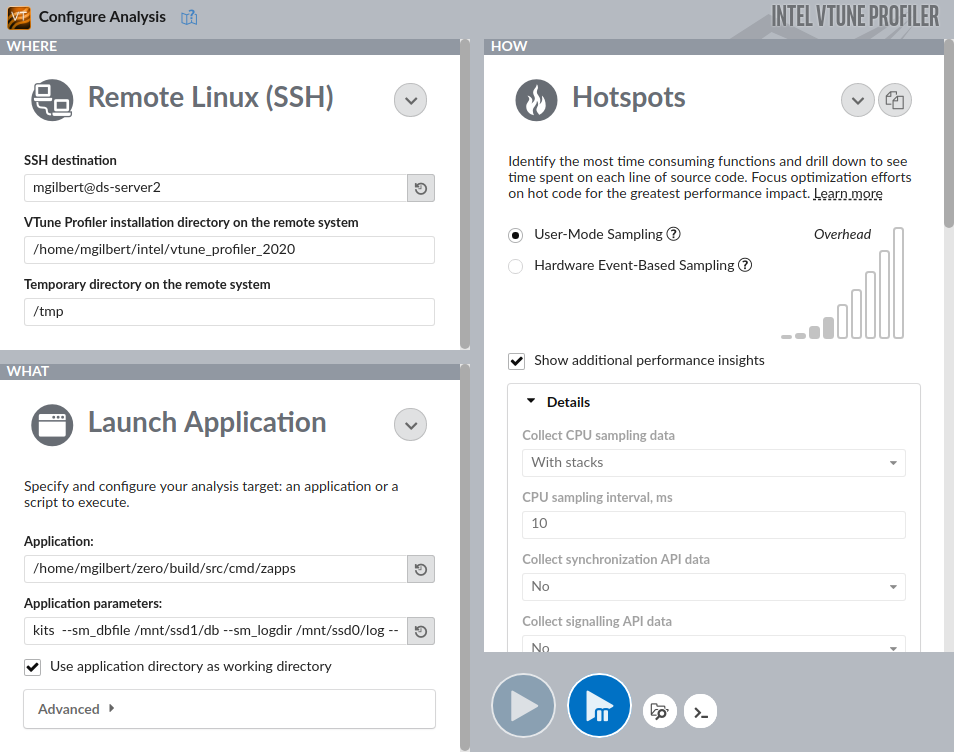
\includegraphics[width = \textwidth-2pt]{data/Intel_VTune_Profiler_Configure_Analysis.png}%
        }
        \vspace{.125em}
        \caption[Configuration of an analysis with Intel® VTune™ Profiler]{In \textit{Intel® VTune™ Profiler}, the configuration of an analysis via GUI is clearly structured: \textbf{How} should \textbf{what} software running \textbf{where} be analyzed?}
        \label{fig:vtuneconfig}
    \end{figure}
\end{@empty}

    The software allows naming of the generated analyses and their management in \emph{projects}, which makes it easier to keep track of all generated results. But these functionalities are not as comfortable as they could be---an analysis cannot be named during configuration. The results have to be generated first to give it its own name afterwards. And after renaming an analysis, the results must be reloaded by the software---resetting the analysis viewer.

    But before the first analysis can be created, a \emph{license} for the software must be acquired and the \textit{VTune™ Profiler} needs to be installed. The \emph{installation} can be done via command line or GUI. But for example, if the target software is running on a server, only the \emph{sampling driver} needs to be installed there, while it is controlled by a full \textit{VTune™ Profiler} installation on the PC on which the analyses are initiated and evaluated.

    But once the software (and the sampling driver on a potentially separate target system) is installed, the first analysis can be started. Figure \ref{fig:vtuneconfig} shows the \emph{configuration dialog} for a \textit{VTune™ Profiler} analysis via GUI. It is divided into \emph{three main topics}.

\begin{@empty}
    \setlength{\fboxsep}{0pt}%
    \setlength{\fboxrule}{1pt}%
    
    \begin{figure}[h]
        \centering
        \fbox{%
            
\includegraphics[width = .75\textwidth]{data/Intel_VTune_Profiler_Configure_Where.png}%
        }
        \vspace{.75em}
        \caption[Where is the VTune™ Profiler target running?]{The \textit{Intel® VTune™ Profiler} does not only allow the analysis of software running local.}
        \label{fig:vtunewhere}
    \end{figure}
\end{@empty}

    First, it is required to decide \textbf{where} to run the target software on---figure \ref{fig:vtuneconfig} shows the different options. For example, if ``Remote Linux (SSH)'' is selected, as in the example shown in figure \ref{fig:vtuneconfig}, the local \textit{VTune™ Profiler} will connect to the target system, where at least the \emph{sampling driver} must be installed, via \textit{SSH}, conveniently using the user's configuration for SSH connections.

\begin{@empty}
    \setlength{\fboxsep}{0pt}%
    \setlength{\fboxrule}{1pt}%
    
    \begin{figure}[h]
        \centering
        \fbox{%
            
\includegraphics[width = .75\textwidth]{data/Intel_VTune_Profiler_Configure_What.png}%
        }
        \vspace{.75em}
        \caption[What is analyzed by the VTune™ Profiler?]{The \textit{Intel® VTune™ Profiler} can also attach to an already running process to analyze that.}
        \label{fig:vtunewhat}
    \end{figure}
\end{@empty}

    The second decision to be made is the question of \textbf{what} to analyze on the target system by the \textit{VTune™ Profiler}. Figure \ref{fig:vtunewhat} shows the different options. While ``Profile System'' and ``Attach to Process'' can also be used to evaluate a production system, the ``Launch Application'' option is best suited for the measurements performed for this chapter. With this option, the target application is started by the \textit{VTune™ Profiler} and specified parameters are passed to it. Data acquisition can be delayed, and a maximum amount of data or time span for data acquisition can be specified, for example, to omit the start and shutdown procedures of the target application from analysis.

\begin{@empty}
    \setlength{\fboxsep}{0pt}%
    \setlength{\fboxrule}{1pt}%
    
    \begin{figure}[h]
        \centering
        \fbox{%
            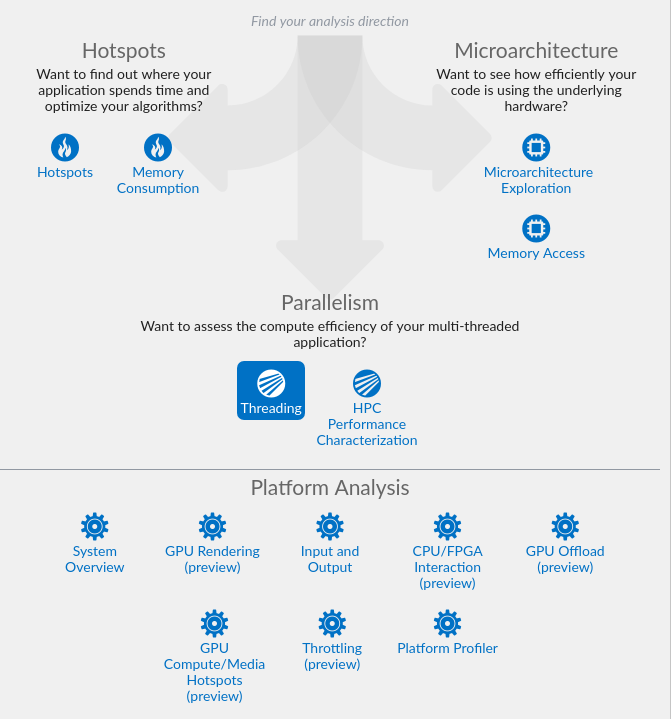
\includegraphics[width = .75\textwidth]{data/Intel_VTune_Profiler_Configure_How.png}%
        }
        \vspace{.75em}
        \caption[How should the VTune™ Profiler analyze the target?]{The \textit{Intel® VTune™ Profiler} offers a number of presets that define which events should be collected during analysis and how this data should be post-processed afterwards.}
        \label{fig:vtunehow}
    \end{figure}
\end{@empty}

    With the final decision, the user tells the \textit{VTune™ Profiler} their intention for the analysis---\textbf{how} should the \textit{VTune™ Profiler} create the analysis? The \textit{Intel® VTune™ Profiler} provides a set of \emph{presets} for various analyses---each preset defines the \emph{events to be counted} and the \emph{sample rate} for \emph{stack traces}, allowing the identification of components, functions, or code lines causing these events.

\begin{@empty}
    \setlength{\fboxsep}{0pt}%
    \setlength{\fboxrule}{1pt}%
    
    \begin{figure}[h!]
        \centering
        \fbox{%
            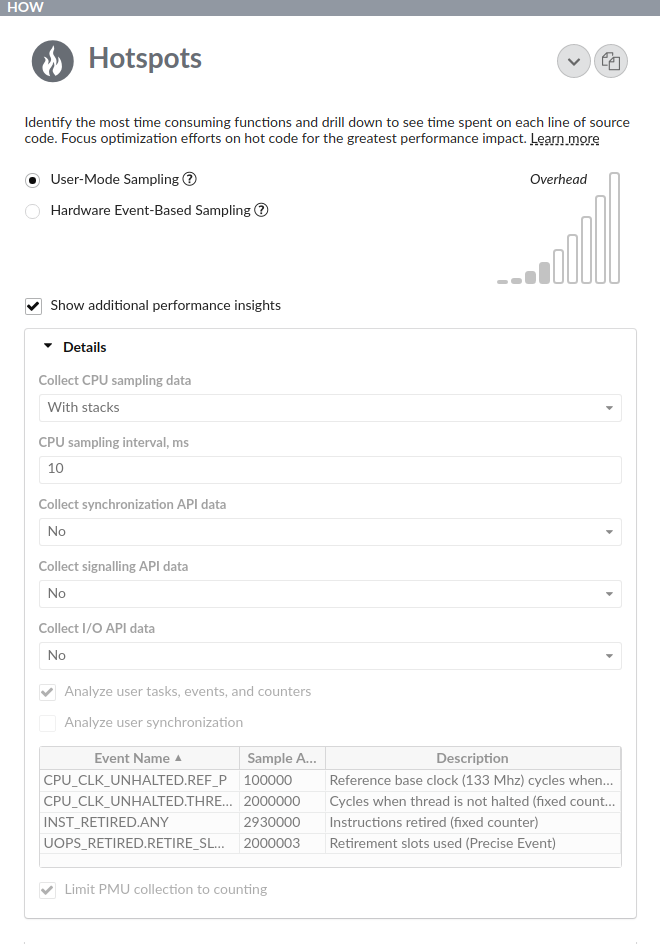
\includegraphics[width = .75\textwidth]{data/Intel_VTune_Profiler_Configure_Hotspots.png}%
        }
        \vspace{.75em}
        \caption[``Hotspots'' preset of the VTune™ Profiler]{The ``Hotspots'' preset of the \textit{Intel® VTune™ Profiler} specifies among many other options the CPU sampling interval and the events to be counted. Many less relevant options that are not used by this preset have been removed from this screenshot.}
        \label{fig:vtunehotspots}
    \end{figure}
\end{@empty}

    The preset  can be used for example with ``User-Mode Sampling'' or with ``Hardware Event-Based Sampling''. ``User-Mode Sampling'' \emph{interrupts} the analyzed process (defined in ``what'') every \SI{10}{\milli\second} (default ``CPU sampling interval'') and stores the current \emph{call stack} of each unhalted thread of the process. The CPU time since the previous sample is then assigned to that captured call stack. Afterwards, the stack trace is \emph{aggregated} by summing the CPU times of identical call stacks to obtain a---statistically exact---allocation of CPU time to different call stacks. ``Hardware Event-Based Sampling'' also interrupts the analyzed process to store the call stacks, but it assigns the values of certain \emph{hardware counters} to each sample, so that different samples contribute to the final summary based on these values. These hardware counters can count e.g. CPU cycles, executed instructions, L2 cache misses or branch mispredictions---depending on the capabilities of the CPU architecture. Figure \ref{fig:vtunehotspots} shows some settings of the ``Hotspots'' preset, but many others, e.g. regarding GPU usage and memory, have been removed from the screenshot for the sake of clarity.

\begin{@empty}
    \setlength{\fboxsep}{0pt}%
    \setlength{\fboxrule}{1pt}%
    
    \begin{figure}[h!]
        \centering
        \fbox{%
            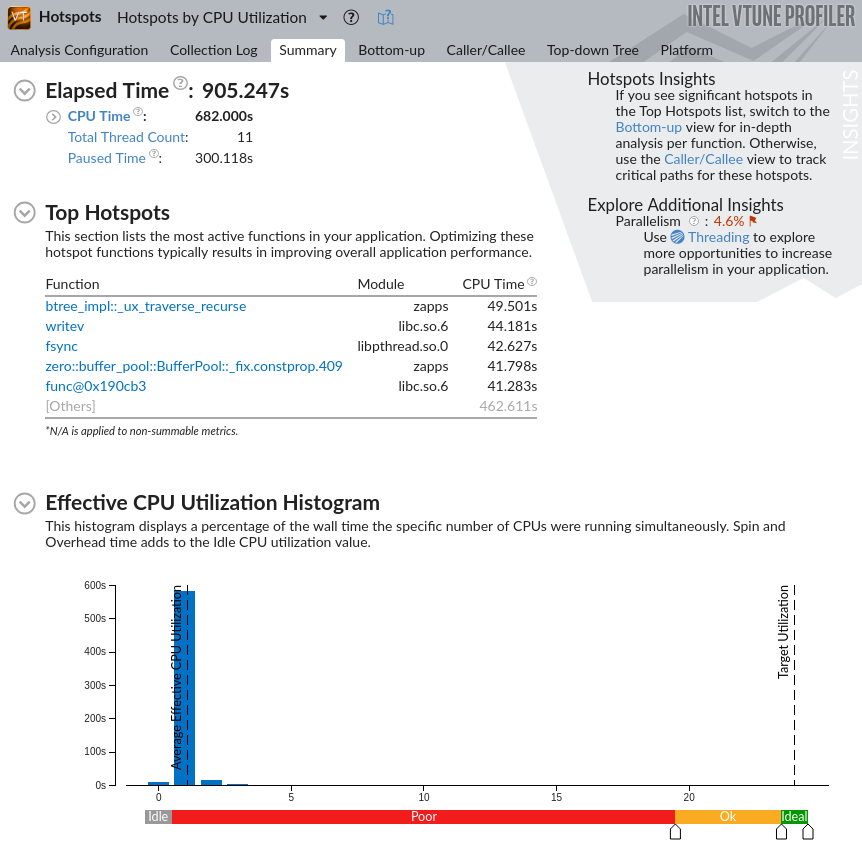
\includegraphics[width = .75\textwidth]{data/Intel_VTune_Profiler_Results_Summary.png}%
        }
        \vspace{.75em}
        \caption[Summary of an analysis done by the VTune™ Profiler]{The \textit{Intel® VTune™ Profiler} provides a ``Summary'' tab for each analysis performed, displaying---depending on configuration---highlights related to various performance aspects.}
        \label{fig:vtunesummary}
    \end{figure}
\end{@empty}

    The \textit{VTune™ Profiler} presents the results of each analysis in a variety of ways, divided among different tabs. An exemplary ``Summary'' tab of the ``Hotspots'' preset when using ``User-Mode Sampling'' is shown in figure \ref{fig:vtunesummary}. It shows a \emph{ranking of the functions} that required the most CPU time and a visualization of the \emph{degree of parallelism} achieved.

\begin{@empty}
    \setlength{\fboxsep}{0pt}%
    \setlength{\fboxrule}{1pt}%
    
    \begin{figure}[h!]
        \centering
        \fbox{%
            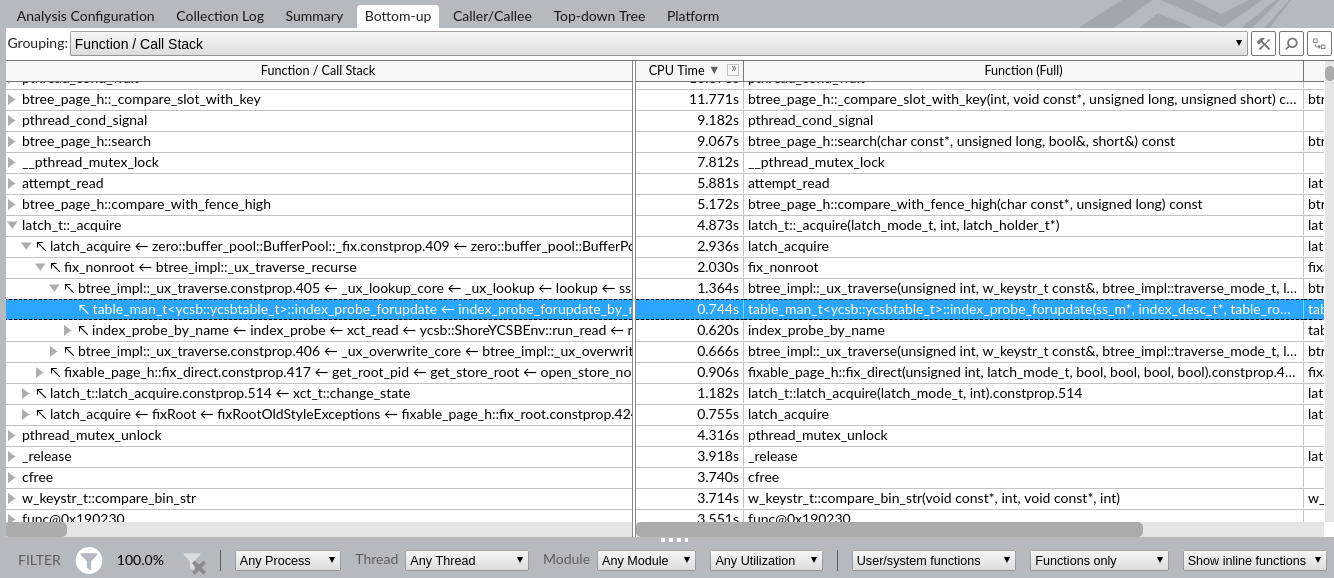
\includegraphics[width = \textwidth]{data/Intel_VTune_Profiler_Results_BottomUp.png}%
        }
        \vspace{.75em}
        \caption[Bottom-up view of an analysis done by the VTune™ Profiler]{The ``Bottom-up'' tab of a \textit{Intel® VTune™ Profiler} analysis summarizes the collected samples based on the lowest element of the call stacks.}
        \label{fig:vtunebottomup}
    \end{figure}
\end{@empty}

    The ``Bottom-up'' tab breaks down CPU time (or other performance characteristics) based on the \emph{bottom element of the call stack} of each sample. This element is the function (or loop, if displayed) that was running on the CPU at the time the sample was taken. As shown in the figure \ref{fig:vtunebottomup}, the callers (and their callers) to these functions can also be displayed along with a breakdown of the share of CPU time of each combination.

    The samples considered for the summaries in the ``Bottom-up'' tab and the other tabs can be \emph{filtered} by timestamp, process, thread and software module. These filter options are shown at the bottom of the figure \ref{fig:vtunebottomup}.

\begin{@empty}
    \setlength{\fboxsep}{0pt}%
    \setlength{\fboxrule}{1pt}%
    
    \begin{figure}[h!]
        \centering
        \fbox{%
            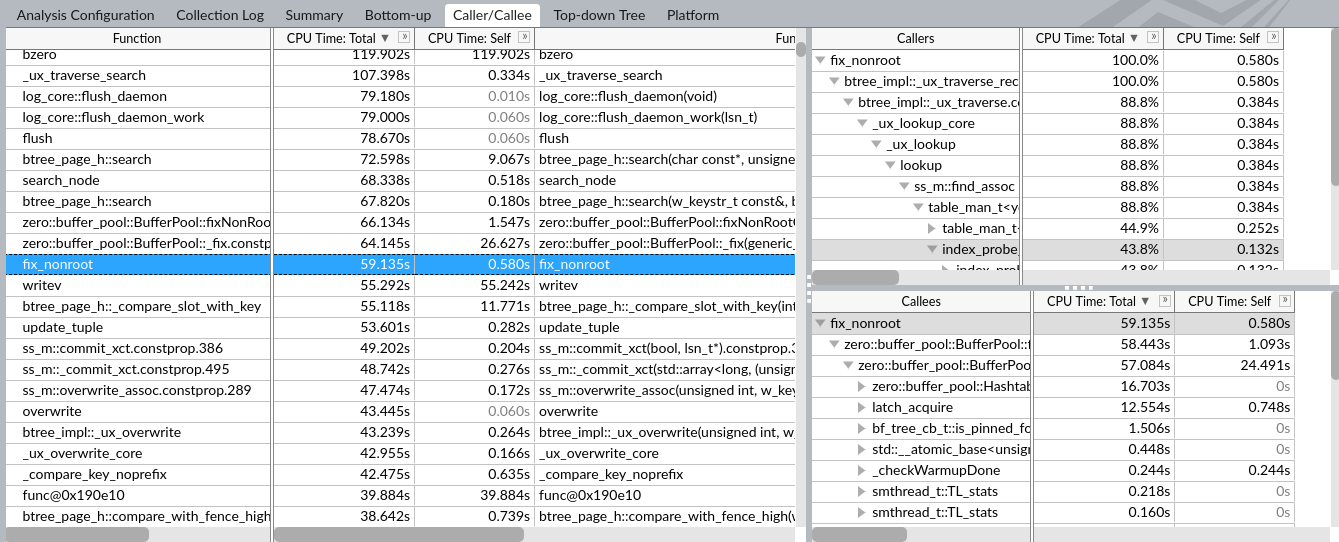
\includegraphics[width = \textwidth]{data/Intel_VTune_Profiler_Results_CallerCallee.png}%
        }
        \vspace{.75em}
        \caption[Caller/Callee view of an analysis done by the VTune™ Profiler]{The ``Caller/Callee'' tab of a \textit{Intel® VTune™ Profiler} analysis lists the total CPU time used by each function---including the called functions.}
        \label{fig:vtunecallercallee}
    \end{figure}
\end{@empty}

    The ``Caller/Callee'' tab lists \emph{each function contained in the stack trace} and assigns it the CPU time it requires including that of any functions it calls. Therefore, the entry point of the program is usually the function with the highest CPU time required---it is the base of every call and every thread spawn. This list is shown in the \emph{left frame} in figure \ref{fig:vtunecallercallee}. The callers and callees to these functions can then be retrieved as shown for \lstinline|fix_nonroot| in the example. The \emph{upper right frame} in the figure shows the callers as they are displayed in the ``Bottom-up'' tab. The callees can be displayed in the same way as they are shown in the ``Top-down Tree'' tab. This is shown in the \emph{lower right frame} in figure \ref{fig:vtunecallercallee}.

\begin{@empty}
    \setlength{\fboxsep}{0pt}%
    \setlength{\fboxrule}{1pt}%
    
    \begin{figure}[h!]
        \centering
        \fbox{%
            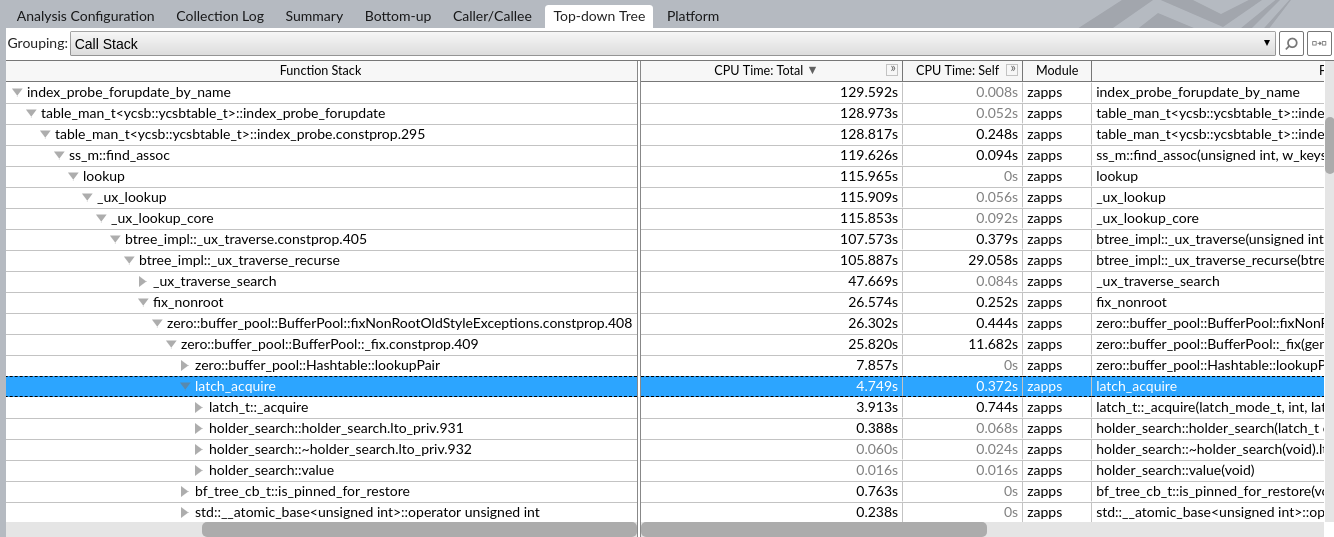
\includegraphics[width = \textwidth]{data/Intel_VTune_Profiler_Results_TopDownTree.png}%
        }
        \vspace{.75em}
        \caption[Top-down view of an analysis done by the VTune™ Profiler]{The ``Top-down Tree'' tab of a \textit{Intel® VTune™ Profiler} analysis offers the possibility to interactively discover the call stack of a program from top to bottom, sorted by e.g. CPU time.}
        \label{fig:vtunetopdowntree}
    \end{figure}
\end{@empty}

    The ``Top-down Tree'' tab initially shows only the entry point of the analyzed program and the total CPU time it has used during the analysis. From there, the view can be \emph{expanded}, as shown in figure \ref{fig:vtunetopdowntree}, to show all called functions (and the functions they call, etc.) together with the CPU time they utilize (including or excluding their callees).

\begin{@empty}
    \setlength{\fboxsep}{0pt}%
    \setlength{\fboxrule}{1pt}%
    
    \begin{figure}[h!]
        \centering
        \fbox{%
            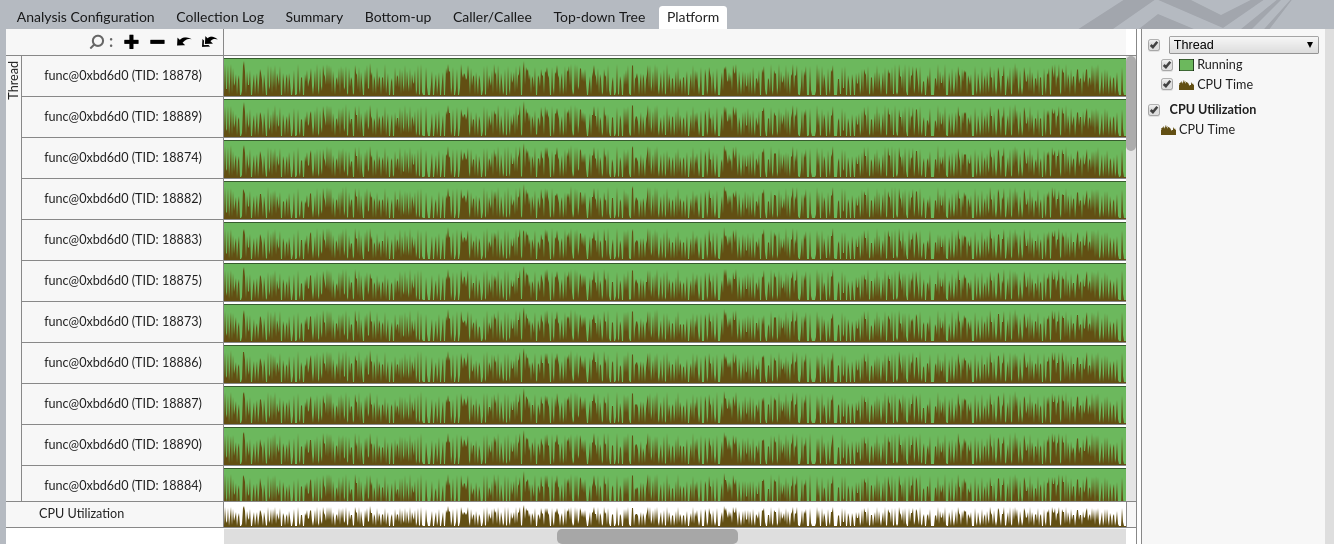
\includegraphics[width = \textwidth]{data/Intel_VTune_Profiler_Results_Platform.png}%
        }
        \vspace{.75em}
        \caption[Platform view of an analysis done by the VTune™ Profiler]{The ``Platform'' tab of a \textit{Intel® VTune™ Profiler} analysis visualizes e.g. the CPU utilization (and optionally spin time of spinlocks) per thread, process or module.}
        \label{fig:vtuneplatform}
    \end{figure}
\end{@empty}

    Finally, the ``Platform'' tab visualizes the complete analysis in terms of \emph{CPU usage}. As shown in figure \ref{fig:vtuneplatform}, it shows a graph for each thread (or alternatively process, module, or any combination of them), with CPU time displayed in brown and idle time in green. For example, if ``synchronization API data'' is collected, the spin time of spinlocks would be displayed in the graphs in red.

\subsubsection{Flaws}

    While collecting measurements for the section \ref{sec:looking_glass}, the \textit{Intel® VTune™ Profiler} showed some of its flaws.

    When ``Launch Application'' is used, it starts the target application and shows the command line output of this program during the tracing. However, this command line output is not saved together with the trace data and thus discarded when the analysis results are closed. If anything from the command line output of the analyzed program is to be used later with the analysis results---such as transaction throughput in the case of \textit{Zero}---this information must be stored outside the \textit{VTune™ Profiler}.

\section{Measurements of Harizopoulos et al. -- Redone} \label{sec:looking_glass}

    Based on the estimation that the assumptions of Harizopoulos et al. and their methodology are too restrictive, in this section their measurements are repeated with \emph{changed assumptions} and using a \emph{completely different technique}. Subsection \ref{subsec:looking_glass_methodology} describes in detail the methodology used and to demonstrate that the----probably most controversial---assumption from \cite{Harizopoulos:2008}----the unnecessity for multithreaded execution of OLTP DBS---is invalid, subsection \ref{subsec:looking_glass_single_threaded} shows the new evaluation (mostly) single-threaded while subsection \ref{subsec:looking_glass_multi_threaded} uses multithreaded execution to provide data for a comparison.

    Due to the extensive evaluation of the effect of the buffer pool size on OLTP performance in Chapter \ref{ch:page_evictioners} and the fact that today larger-than-memory databases are rarely used, \emph{only in-memory DBSs} are considered in these measurements. Since \emph{transaction support} and \emph{ACID guarantees} are still used in most OLTP applications, these are also used during the measurements. \emph{ARIES-style logging} is also used, as this is still common and built into the used prototype DBMS.

\subsection{Methodology} \label{subsec:looking_glass_methodology}

    The software used to breakdown the runtime of an OLTP system is the \emph{Intel® VTune™ Profiler 2020}, which is described in subsection \ref{subsec:vtune}. It was configured according to the outlined configuration steps as follows:

\begin{description}
    \item[Where]    The DBS was running on a ``Remote Linux (SSH)'' server. Its configuration is described in subsection \ref{subsec:page_evictioners_system_configuration}.
    \item[What]     The DBS with built-in benchmarks was started by the profiling software. Some details about the embedded DBMS used---\textit{Zero}---were given in the subsection \ref{subsec:page_evictioners_limits} and the benchmarks are \textit{TPC-C} (see subsection \ref{subsec:page_evictioners_benchmark}) and \textit{YCSB} (see subsection \ref{subsubsec:looking_glass_benchmark}). The DBS started with a clean DB (no crash recovery required), but---obviously---with an empty buffer pool. Due to the fact that a typical DBMS runs continuously---and thus with a populated buffer pool---the \textit{Intel® VTune™ Profiler} started tracing after a cold start of \SI{5}{\minute} (recording \SI{10}{\minute} total) to give realistic results.
    \item[How]      The preset ``Hotspots'' of the \textit{Intel® VTune™ Profiler} was used.
\end{description}

    The software profile generated by the \textit{Intel® VTune™ Profiler} consists of stack traces, as shown in subsection \ref{subsec:vtune}, with a total run time in seconds for each of them. Every relevant (except e.g. benchmark code such as the test data generation that would typically run on a client) stack trace is then \emph{manually assigned to one of the DBMS components} described in subsection \ref{subsubsec:looking_glass_components}. The delayed start of tracing and the overhead associated with it prevent a reliable calculation of the CPU time per transaction, so that only the percentage of CPU time used per component is shown.

\subsubsection{Benchmarks} \label{subsubsec:looking_glass_benchmark}

    The first benchmark used for the measurements in this chapter is the \emph{Yahoo! Cloud Serving Benchmark}\footnote{\url{https://ycsb.site/}} (\textit{YCSB}). It is based on a simple workload for key-value stores (\emph{NoSQL DBMSs}) and was designed for systems running in the cloud. It is for NoSQL DBMSs what \textit{TPC-C} is for OLTP SQL DBMSs.

    The DB contains \num{10000000} completely random \emph{key-value pairs} in a table with 10 character fields of \SI{100}{\byte} each mapped to a \SI{10}{\byte} key. One \emph{skewed} (based on the Zipfian distribution) random key is drawn per transaction. A read transaction reads all 10 fields associated with the key and an update transaction writes random data to a randomly selected field associated with the key. The read-only \textit{YCSB} workloads from subsection \ref{subsubsec:looking_glass_single_threaded_read_only_ycsb} and \ref{subsubsec:looking_glass_multi_threaded_read_only_ycsb} execute only read transactions, the write-only ones from subsection \ref{subsubsec:looking_glass_single_threaded_write_only_ycsb} and \ref{subsubsec:looking_glass_multi_threaded_write_only_ycsb} execute only update transactions. No transactions abort and all queried keys exist in the DB.

    The second benchmark used in this chapter---\textit{TPC-C}---performs read and (more frequently) update transactions, so that a read-write \textit{YCSB} workload is evaluated. The database and transactions of \textit{TPC-C} have already been described in the subsection \ref{subsec:page_evictioners_benchmark}.

\subsubsection{Considered DBMS Components} \label{subsubsec:looking_glass_components}

\begin{description}
    \item[B-Tree]       Each stack trace associated with maintaining the \emph{Foster B-Tree} structure or searching for keys within a B-Tree page is assigned to this component.
    \item[Logging]      The CPU time used to create log records, maintain log sequence numbers (LSNs) and flush log records to SSD is assigned to this component.
    \item[Locking]      The CPU time spent on \emph{transaction management}, acquiring and releasing locks and managing locks in the \emph{lock manager} is assigned to this component.
                        \begin{description}
                            \item[Latching] \emph{Internal structures} of transaction and lock managers require latches (not the mutexes on which the locks are based on) for synchronization in multithreaded environments. The CPU time required to acquire and release these latches is assigned to this sub-component.
                        \end{description}
    \item[Buffer Pool]  The effort for \emph{fixing and unfixing pages} is assigned to this component. In addition to the following sub-components, page eviction would also be a sub-component, but only the RANDOM page replacement algorithm and smaller-than-memory DBs are considered thus requiring no CPU time for page eviction.
                        \begin{description}
                            \item[Latching]     A latch is assigned to \emph{each buffer frame}, and a thread reading or writing a page must acquire the corresponding latch in the appropriate mode (shared or exclusive). The CPU time required to acquire and release these latches is assigned to this sub-component.
                            \item[Fetching]     Few \emph{pages are fetched from the SSD} while the stack traces are being gathered, because---due to the skewed access to the records---not all pages were accessed during the cold start phase, which is ignored by the profiler. But since the whole database fits into the buffer pool during each benchmark run, no pages need to be fetched because they were previously evicted. The CPU time required to fetch pages from the SSD is assigned to this sub-component.
                            \item[Hash Table]   The hash table \emph{maps the page identifier of each page in the buffer pool to the corresponding buffer frame index}. It is queried on each page fix---regardless of whether it is a page hit or a page miss. The runtime required to search within this hash table is assigned to this sub-component. More details about the hash table and an alternative can be found in the subsection \ref{subsec:looking_glass_swizzling}.
                            \item[Free List]    The free list is a simple concurrent \emph{queue} containing the \emph{indexes of unoccupied buffer frames}. Indexes are only dequeued when a page is fetched from SSD, so the CPU time assigned to this sub-component is very little.
                        \end{description}
\end{description}

    The \emph{logical access paths} layer, which is responsible for the mapping between internal and external records, among other things, and which is not a core component of \textit{Zero}, is not considered here. It consumes up to \SI{25}{\percent} of the CPU time, but mainly for memory operations, e.g. for creating records based on input data, so these operations would be considered \emph{useful work} by Harizopoulos et al.

\subsection{Other Related Work} \label{subsec:looking_glass_related_work}

    In contrast to Harizopoulos et al., Johnson et al. focus in \cite{Johnson:2009} on scalability in the context of multithreading. They present their successor of the \emph{Shore Storage Manager}---\textit{Shore-MT}---together with measurements to prove its better multithreading capabilities. Instead of removing modules of the \textit{Shore Storage Manager} one by one, they \emph{optimized them one after the other} and showed the increase in transaction throughput (for a simple insert-only microbenchmark) after each step. In this way, their measurements show which components of \textit{Shore Storage Manager} limit scalability to what extent.

    Pandis et al. proposed a new page latching protocol for partitioned DBSs. In their work, they compared their approach---physiological partitioning (PLP)---to the ``conventional'' approach, by breaking down the \emph{number of critical sections} per DBMS component.

    The most detailed analysis of the inner workings of a DBMS in terms of performance was conducted by Tözün et al. in \cite{Tozun:2013}. Their main goal was to compare the (micro-architectural) behavior of the OLTP benchmarks of the \emph{Transaction Processing Performance Council}---\textit{TPC-B}, \textit{TPC-C} and \textit{TPC-E}. They broke down \emph{CPU time} and \emph{other performance metrics per DBMS component} in a very similar way as here, compared CPU cache misses per cache level, and compared the behavior of the three benchmarks on systems that use \emph{Hyper-Threading Technology}.

\subsection{Single-Threaded OLTP System Analysis} \label{subsec:looking_glass_single_threaded}

    The analysis of single-threaded OLTP systems is especially relevant for the comparisons between the results of Harizopoulos et al. and the results presented here, which were obtained using a totally different methodology. However, the results can also give a better insight---compared to the results for multithreaded OLTP systems from subsection \ref{subsec:looking_glass_multi_threaded}---into the \emph{overhead of the pessimistic concurrency control}, because here---without multithreaded and interleaved execution---every operation performed by the lock manager is unnecessary.

\begin{@empty}
    \pgfplotsset{%
        every axis/.append style = {
            ylabel near ticks,
            y label style = {font = \small},
            yticklabel style = {font = \scriptsize},
            ymode = log,
            scaled y ticks = false,
            ybar = .8pt,
            xmin = -0.75,
            xmax = 2.75,
            bar width = 1.5em,
            xtick style = {draw = none},
            xtick = {0, 1, 2},
            xticklabels = {{\makecell[c]{read-only\\YCSB}}, {\makecell[c]{update-only\\YCSB}}, {\makecell[c]{\textit{TPC-C}}}},
            x tick label style = {align = center,
                                  font = \footnotesize},
            xlabel near ticks,
            x label style = {font = \small},
            ymajorgrids = true,
            legend entries = {{1 Thread}, {12 Threads}, {24 Threads}},
            legend style = {font = \footnotesize,
                            legend columns = 1,
                            /tikz/every even column/.append style = {column sep = 0.5cm}},
            width = .8\textwidth,
            height = .4\textheight
        }
    }
    
    \tikzset{%
        1thread/.style = {thick},
        12threads/.style = {thick},
        24threads/.style = {thick}
    }
    
    \nottoggle{bwmode}{
        \tikzset{%
            1thread/.append style = {draw = Cyan, fill = Cyan!25},
            12threads/.append style = {draw = Cyan, fill = Cyan!50},
            24threads/.append style = {draw = Cyan, fill = Cyan!75}
        }
    }{
        \tikzset{%
            1thread/.append style = {draw = black, fill = black!25},
            12threads/.append style = {draw = black, fill = black!50},
            24threads/.append style = {draw = black, fill = black!75}
        }
    }
    
    \begin{figure}[t]
        \centering
        \begin{tikzpicture}
            \begin{axis}[ylabel = {$\text{Transaction throughput }\left[\si{1\per\minute}\right]$},
                         legend pos = north east]
                \addplot[1thread] coordinates
                    {(0, 7313398.8) (1, 5355238.2) (2, 203286.69)};
                \addplot[12threads] coordinates
                    {(0, 16913852.4) (1, 5403291) (2, 900337.11)};
                \addplot[24threads] coordinates
                    {(0, 14604468.6) (1, 5083255.2) (2, 905283.53)};
            \end{axis}
        \end{tikzpicture}
        \caption[Transaction throughput for different thread counts]{Transaction throughput for different numbers of working threads for read/update-only \textit{YCSB} and \textit{TPC-C}}
        \label{fig:threadsthroughput}
    \end{figure}
\end{@empty}

    A quick comparison of the transaction throughput achieved with \emph{different numbers of working threads}---i.e., different numbers of threads processing transactions \emph{concurrently} and different numbers of transactions executing in an \emph{interleaved} fashion---is shown in figure \ref{fig:threadsthroughput}. The used server (see subsection \ref{subsec:page_evictioners_system_configuration}) is equipped with two CPUs, each with 6 cores, supporting 2 hardware contexts running concurrently via simultaneous multithreading, so that a total of 24 \emph{logical cores} or 12 \emph{physical cores} are available.

    The results indicate that the \emph{additional logical cores} cannot be used to increase transaction throughput. In fact, they even increase overhead through more contention and additional context switches. But \emph{read-only} \textit{YCSB} and especially \textit{TPC-C} benefit from multithreaded and interleaved transaction execution. \emph{Read-only} \textit{YCSB} can more than double its throughput if 12 instead of 1 working threads are used, \textit{TPC-C} can more than quadruple its throughput. The bottleneck of \emph{read-only} \textit{YCSB} is the contention caused by the very large number of very short transactions on a global latch in the transaction manager, which has to be acquired twice per transaction. The limited write rate of the transaction log prevents an increase in transaction throughput for \emph{update-only} \textit{YCSB}. The more balanced workload of \textit{TPC-C} can better utilize the larger number of working threads.

\subsubsection{Read-Only YCSB} \label{subsubsec:looking_glass_single_threaded_read_only_ycsb}

\begin{@empty}
    \pgfplotsset{%
        every axis/.append style = {
            ylabel = {CPU cycles $\left[\si{\percent}\right]$},
            ybar stacked,
            ylabel near ticks,
            y label style = {font = \small},
            ylabel shift = -.5em,
            ymode = normal,
            ymin = 0,
            ymax = 100,
            yticklabel style = {font = \scriptsize},
            ymode = normal,
            scaled y ticks = false,
            xmin = -0.25,
            xmax = 0.25,
            xtick = \empty,
            bar width = 0.5,
            ymajorgrids = false,
            width = .375\textwidth,
            height = .625\textheight
        }
    }

    \nottoggle{bwmode}{
        \tikzset{%
            a0/.style = {black, fill = cyan},
            a1/.style = {black, fill = cyan!80},
            a2/.style = {black, fill = cyan!60},
            a3/.style = {black, fill = cyan!40},
            a4/.style = {black, fill = cyan!20},
            b0/.style = {black, fill = magenta},
            b1/.style = {black, fill = magenta!50},
            d/.style = {black, fill = white}
        }
    }{
        \tikzset{%
            a0/.style = {black, pattern color = black!25, pattern = {Lines[angle = 45, distance = 2pt]}},
            a1/.style = {black, pattern color = black!25, pattern = {Lines[angle = 45, distance = 4pt]}},
            a2/.style = {black, pattern color = black!25, pattern = {Lines[angle = 45, distance = 6pt]}},
            a3/.style = {black, pattern color = black!25, pattern = {Lines[angle = 45, distance = 8pt]}},
            a4/.style = {black, pattern color = black!25, pattern = {Lines[angle = 45, distance = 10pt]}},
            b0/.style = {black, pattern color = black!25, pattern = {Lines[angle = -45, distance = 5pt]}},
            b1/.style = {black, pattern color = black!25, pattern = {Lines[angle = -45, distance = 10pt]}},
            d/.style = {black, fill = white}
        }
    }

    \begin{figure}[h!]
        \centering
        \begin{tikzpicture}[remember picture]
            \begin{axis}[ymax = 100]
                \node[] at ($(0, 0)!.5!(0, 8.27+0.13+4.44+4.14+5.30)$) {\makecell[c]{\contour{white}{Buffer pool}\\\footnotesize \contour{white}{\SI{22.28}{\percent}}}};
                \node[] at ($(0, 8.27+0.13+4.44+4.14+5.30)!.5!(0, 8.27+0.13+4.44+4.14+5.30+32.09+2.38)$) {\makecell[c]{\contour{white}{Locking}\\\footnotesize \contour{white}{\SI{34.47}{\percent}}}};
                \node[] at ($(0, 8.27+0.13+4.44+4.14+5.30+32.09+2.38)!.5!(0, 8.27+0.13+4.44+4.14+5.30+32.09+2.38+1.01)$) {\scriptsize\makecell[c]{\contour{white}{Logging \SI{1.01}{\percent}}}};
                \node[] at ($(0, 8.27+0.13+4.44+4.14+5.30+32.09+2.38+1.01)!.5!(0, 8.27+0.13+4.44+4.14+5.30+32.09+2.38+1.01+42.24)$) {\makecell[c]{\contour{white}{B-tree}\\\footnotesize \contour{white}{\SI{42.24}{\percent}}}};
        
                \addplot[d] coordinates          {(0, 0)};
                \addplot[a4]  coordinates       {(0, 8.27)};
                \addplot[a3]  coordinates       {(0, 0.13)};
                \addplot[a2]  coordinates       {(0, 4.44)};
                \addplot[a1]  coordinates       {(0, 4.14)};
                \addplot[a0] coordinates       {(0, 5.30)};
                \addplot[b1]  coordinates    {(0, 32.09)};
                \addplot[b0] coordinates    {(0, 2.38)};
                \addplot[a0] coordinates           {(0, 1.01)};
                \addplot[b0] coordinates        {(0, 42.24)};
        
                \coordinate (0rest)            at (0.25, 0);
                \coordinate (0bufferRest)      at (0.25, 8.27);
                \coordinate (0bufferFreeList)  at (0.25, 8.27+0.13);
                \coordinate (0bufferHashTable) at (0.25, 8.27+0.13+4.44);
                \coordinate (0bufferFetching)  at (0.25, 8.27+0.13+4.44+4.14);
                \coordinate (0bufferLatching)  at (0.25, 8.27+0.13+4.44+4.14+5.30);
                \coordinate (0lockingRest)     at (0.25, 8.27+0.13+4.44+4.14+5.30+32.09);
                \coordinate (0lockingLatching) at (0.25, 8.27+0.13+4.44+4.14+5.30+32.09+2.38);
            \end{axis}
        \end{tikzpicture}
        \hspace{4em}
        \begin{tikzpicture}[remember picture]
            \begin{axis}[ylabel = { },
                         ymax = 8.27+0.13+4.44+4.14+5.30+32.09+2.38]
                \node[] at ($(0, 8.27)!.5!(0, 8.27+0.13)$)  {\scriptsize\makecell[c]{\contour{white}{Free list \SI{0.13}{\percent}}}};
                \node[] at ($(0, 8.27+0.13)!.5!(0, 8.27+0.13+4.44)$) {\scriptsize\makecell[c]{\contour{white}{Hash table \SI{4.44}{\percent}}}};
                \node[] at ($(0, 8.27+0.13+4.44)!.5!(0, 8.27+0.13+4.44+4.14)$){\scriptsize\makecell[c]{\contour{white}{Fetching} \contour{white}{\SI{4.14}{\percent}}}};
                \node[] at ($(0, 8.27+0.13+4.44+4.14)!.5!(0, 8.27+0.13+4.44+4.14+5.30)$){\makecell[c]{\contour{white}{Latching}\\\footnotesize \contour{white}{\SI{5.3}{\percent}}}};
                \node[anchor = north, inner ysep = .5pt] at (0, 8.27+0.13+4.44+4.14+5.30+32.09+2.38){\scriptsize\makecell[c]{\contour{white}{Latching \SI{2.38}{\percent}}}};
        
                \addplot[a4]  coordinates       {(0, 8.27)};
                \addplot[a3]  coordinates       {(0, 0.13)};
                \addplot[a2]  coordinates       {(0, 4.44)};
                \addplot[a1]  coordinates       {(0, 4.14)};
                \addplot[a0] coordinates       {(0, 5.30)};
                \addplot[b1]  coordinates    {(0, 32.09)};
                \addplot[b0] coordinates    {(0, 2.38)};
        
                \coordinate (1rest)            at (-0.25, 0);
                \coordinate (1bufferRest)      at (-0.25, 8.27);
                \coordinate (1bufferFreeList)  at (-0.25, 8.27+0.13);
                \coordinate (1bufferHashTable) at (-0.25, 8.27+0.13+4.44);
                \coordinate (1bufferFetching)  at (-0.25, 8.27+0.13+4.44+4.14);
                \coordinate (1bufferLatching)  at (-0.25, 8.27+0.13+4.44+4.14+5.30);
                \coordinate (1lockingRest)     at (-0.25, 8.27+0.13+4.44+4.14+5.30+32.09);
                \coordinate (1lockingLatching) at (-0.25, 8.27+0.13+4.44+4.14+5.30+32.09+2.38);
            \end{axis}
        \end{tikzpicture}
        \begin{tikzpicture}[remember picture,
                            overlay]
            \draw (0rest)[draw = black]            -- (1rest);
            \draw (0bufferRest)[draw = black]      -- (1bufferRest);
            \draw (0bufferFreeList)[draw = black]  -- (1bufferFreeList);
            \draw (0bufferHashTable)[draw = black] -- (1bufferHashTable);
            \draw (0bufferFetching)[draw = black]  -- (1bufferFetching);
            \draw (0bufferLatching)[draw = black]  -- (1bufferLatching);
            \draw (0lockingRest)[draw = black]     -- (1lockingRest);
            \draw (0lockingLatching)[draw = black] -- (1lockingLatching);
        \end{tikzpicture}
        \caption[CPU cycles breakdown for single-threaded read-only YCSB]{Component-wise breakdown of the CPU cycles when running read-only \textit{YCSB} with one querying terminal.}
        \label{fig:cyclesycsbread1}
    \end{figure}
\end{@empty}

    Figure \ref{fig:cyclesycsbread1} shows the breakdown of CPU time of \textit{Zero} when running \emph{read-only} \textit{YCSB} on 1 working thread and a DB smaller than the buffer pool. While this diagram only shows the percentage of CPU time per DBMS component, CPU times in seconds are given in table \ref{tab:breakdown} later in this section.

    Since \emph{read-only} workloads do not generate log entries, \emph{logging} here only accounts for \SI{1.01}{\percent} of the total CPU time. The only overhead of the transaction log is caused by the need to store the current LSN for each transaction at the time it begins.

    The \SI{4.14}{\percent} of CPU time used to \emph{fetch pages} from the SSD (and the \SI{0.13}{\percent} used to access the buffer pool's free list) is \emph{caused by the skewed DB accesses} of \textit{YCSB} where not all pages used during the benchmark run were referenced during the buffer pool warmup.

    Because of the very large number of simple transactions that are being executed, the lock manager and mainly the \emph{transaction manager} use \SI{34.47}{\percent} of CPU time. This overhead is caused by management tasks required whenever a transaction begins or commits.

    During single-threaded execution, no concurrency control is required, so \emph{lock management} and \emph{buffer frame latching}---which accounts for \SI{5.3}{\percent} of CPU time---are a waste of resources.

\subsubsection{Write-Only YCSB} \label{subsubsec:looking_glass_single_threaded_write_only_ycsb}

\begin{@empty}
    \pgfplotsset{%
        every axis/.append style = {
            ylabel = {CPU cycles $\left[\si{\percent}\right]$},
            ybar stacked,
            ylabel near ticks,
            y label style = {font = \small},
            ylabel shift = -.5em,
            ymode = normal,
            ymin = 0,
            ymax = 100,
            yticklabel style = {font = \scriptsize},
            ymode = normal,
            scaled y ticks = false,
            xmin = -0.25,
            xmax = 0.25,
            xtick = \empty,
            bar width = 0.5,
            ymajorgrids = false,
            width = .375\textwidth,
            height = .625\textheight
        }
    }

    \nottoggle{bwmode}{
        \tikzset{%
            a0/.style = {black, fill = cyan},
            a1/.style = {black, fill = cyan!80},
            a2/.style = {black, fill = cyan!60},
            a3/.style = {black, fill = cyan!40},
            a4/.style = {black, fill = cyan!20},
            b0/.style = {black, fill = magenta},
            b1/.style = {black, fill = magenta!50},
            d/.style = {black, fill = white}
        }
    }{
        \tikzset{%
            a0/.style = {black, pattern color = black!25, pattern = {Lines[angle = 45, distance = 2pt]}},
            a1/.style = {black, pattern color = black!25, pattern = {Lines[angle = 45, distance = 4pt]}},
            a2/.style = {black, pattern color = black!25, pattern = {Lines[angle = 45, distance = 6pt]}},
            a3/.style = {black, pattern color = black!25, pattern = {Lines[angle = 45, distance = 8pt]}},
            a4/.style = {black, pattern color = black!25, pattern = {Lines[angle = 45, distance = 10pt]}},
            b0/.style = {black, pattern color = black!25, pattern = {Lines[angle = -45, distance = 5pt]}},
            b1/.style = {black, pattern color = black!25, pattern = {Lines[angle = -45, distance = 10pt]}},
            d/.style = {black, fill = white}
        }
    }
    
    \begin{figure}[h!]
        \centering
        \begin{tikzpicture}[remember picture]
            \begin{axis}[ymax = 100]
                \node[] at ($(0, 0)!.5!(0, 6.17+0.07+3.46+1.17+5.17)$) {\makecell[c]{\contour{white}{Buffer pool}\\\footnotesize \contour{white}{\SI{16.04}{\percent}}}};
                \node[] at ($(0, 6.17+0.07+3.46+1.17+5.17)!.5!(0, 6.17+0.07+3.46+1.17+5.17+19.19+2.54)$) {\makecell[c]{\contour{white}{Locking}\\\footnotesize \contour{white}{\SI{21.73}{\percent}}}};
                \node[] at ($(0, 6.17+0.07+3.46+1.17+5.17+19.19+2.54)!.5!(0, 6.17+0.07+3.46+1.17+5.17+19.19+2.54+24.42)$) {\makecell[c]{\contour{white}{Logging}\\\footnotesize \contour{white}{\SI{24.42}{\percent}}}};
                \node[] at ($(0, 6.17+0.07+3.46+1.17+5.17+19.19+2.54+24.42)!.5!(0, 6.17+0.07+3.46+1.17+5.17+19.19+2.54+24.42+37.81)$) {\makecell[c]{\contour{white}{B-tree}\\\footnotesize \contour{white}{\SI{37.81}{\percent}}}};
        
                \addplot[d] coordinates          {(0, 0)};
                \addplot[a4]  coordinates       {(0, 6.17)};
                \addplot[a3]  coordinates       {(0, 0.07)};
                \addplot[a2]  coordinates       {(0, 3.46)};
                \addplot[a1]  coordinates       {(0, 1.17)};
                \addplot[a0] coordinates       {(0, 5.17)};
                \addplot[b1]  coordinates    {(0, 19.19)};
                \addplot[b0] coordinates    {(0, 2.54)};
                \addplot[a0] coordinates           {(0, 24.42)};
                \addplot[b0] coordinates        {(0, 37.81)};
        
                \coordinate (0rest)            at (0.25, 0);
                \coordinate (0bufferRest)      at (0.25, 6.17);
                \coordinate (0bufferFreeList)  at (0.25, 6.17+0.07);
                \coordinate (0bufferHashTable) at (0.25, 6.17+0.07+3.46);
                \coordinate (0bufferFetching)  at (0.25, 6.17+0.07+3.46+1.17);
                \coordinate (0bufferLatching)  at (0.25, 6.17+0.07+3.46+1.17+5.17);
                \coordinate (0lockingRest)     at (0.25, 6.17+0.07+3.46+1.17+5.17+19.19);
                \coordinate (0lockingLatching) at (0.25, 6.17+0.07+3.46+1.17+5.17+19.19+2.54);
            \end{axis}
        \end{tikzpicture}
        \hspace{4em}
        \begin{tikzpicture}[remember picture]
            \begin{axis}[ylabel = { },
                         ymax = 6.17+0.07+3.46+1.17+5.17+19.19+2.54]
                \node[] at ($(0, 6.17)!.5!(0, 6.17+0.07)$)  {\scriptsize\makecell[c]{\contour{white}{Free list \SI{0.07}{\percent}}}};
                \node[] at ($(0, 6.17+0.07)!.5!(0, 6.17+0.07+3.46)$) {\scriptsize\makecell[c]{\contour{white}{Hash table \SI{3.46}{\percent}}}};
                \node[] at ($(0, 6.17+0.07+3.46)!.5!(0, 6.17+0.07+3.46+1.17)$){\scriptsize\makecell[c]{\contour{white}{Fetching} \contour{white}{\SI{1.17}{\percent}}}};
                \node[] at ($(0, 6.17+0.07+3.46+1.17)!.5!(0, 6.17+0.07+3.46+1.17+5.17)$){\makecell[c]{\contour{white}{Latching}\\\footnotesize \contour{white}{\SI{5.17}{\percent}}}};
                \node[] at ($(0, 6.17+0.07+3.46+1.17+5.17+19.19)!.5!(0, 6.17+0.07+3.46+1.17+5.17+19.19+2.54)$){\scriptsize\makecell[c]{\contour{white}{Latching \SI{2.54}{\percent}}}};
        
                \addplot[a4]  coordinates       {(0, 6.17)};
                \addplot[a3]  coordinates       {(0, 0.07)};
                \addplot[a2]  coordinates       {(0, 3.46)};
                \addplot[a1]  coordinates       {(0, 1.17)};
                \addplot[a0] coordinates       {(0, 5.17)};
                \addplot[b1]  coordinates    {(0, 19.19)};
                \addplot[b0] coordinates    {(0, 2.54)};
        
                \coordinate (1rest)            at (-0.25, 0);
                \coordinate (1bufferRest)      at (-0.25, 6.17);
                \coordinate (1bufferFreeList)  at (-0.25, 6.17+0.07);
                \coordinate (1bufferHashTable) at (-0.25, 6.17+0.07+3.46);
                \coordinate (1bufferFetching)  at (-0.25, 6.17+0.07+3.46+1.17);
                \coordinate (1bufferLatching)  at (-0.25, 6.17+0.07+3.46+1.17+5.17);
                \coordinate (1lockingRest)     at (-0.25, 6.17+0.07+3.46+1.17+5.17+19.19);
                \coordinate (1lockingLatching) at (-0.25, 6.17+0.07+3.46+1.17+5.17+19.19+2.54);
            \end{axis}
        \end{tikzpicture}
        \begin{tikzpicture}[remember picture,
                            overlay]
            \draw (0rest)[draw = black]            -- (1rest);
            \draw (0bufferRest)[draw = black]      -- (1bufferRest);
            \draw (0bufferFreeList)[draw = black]  -- (1bufferFreeList);
            \draw (0bufferHashTable)[draw = black] -- (1bufferHashTable);
            \draw (0bufferFetching)[draw = black]  -- (1bufferFetching);
            \draw (0bufferLatching)[draw = black]  -- (1bufferLatching);
            \draw (0lockingRest)[draw = black]     -- (1lockingRest);
            \draw (0lockingLatching)[draw = black] -- (1lockingLatching);
        \end{tikzpicture}
        \caption[CPU cycles breakdown for single-threaded update-only YCSB]{Component-wise breakdown of the CPU cycles when running update-only \textit{YCSB} with one querying terminal.}
        \label{fig:cyclesycsbwrite1}
    \end{figure}
\end{@empty}

    Figure \ref{fig:cyclesycsbwrite1} shows the CPU time breakdown of \textit{Zero} when running \emph{update-only} \textit{YCSB} on 1 working thread and a DB smaller than the buffer pool.

    Just like the \emph{read-only} \textit{YCSB}, the \emph{update-only} \textit{YCSB} does not access all used DB pages during buffer pool warmup. However, due to the lower transaction throughput of this workload, significantly fewer pages have to be \emph{fetched} using only $\SI{1.17}{\percent} + \SI{0.07}{\percent}$ of the total CPU time.

    In contrast to \emph{read-only} workloads, each transaction of the \emph{update-only} \textit{YCSB} results in the creation and writing of a log entry, which results in \SI{24.42}{\percent} of the CPU time used for \emph{logging}.

    The just a little smaller number of simple transactions executed with the \emph{update-only} variant causes the \emph{lock and transaction managers} to use \SI{21.73}{\percent} of CPU time. As can be seen in table \ref{tab:breakdown}, the absolute CPU time used by these components reflects what is expected taking into account the transaction throughput and CPU time required during read-only \textit{YCSB}.

    The lower transaction throughput does not reduce the absolute CPU time used by the \emph{Foster B-tree}, although fewer records are accessed. The lower overhead imposed by the \emph{buffer pool}---compared to the measurement with \emph{read-only} \textit{YCSB}---is similar to what would be expected considering the lower transaction throughput.

\subsubsection{TPC-C} \label{subsubsec:looking_glass_single_threaded_tpcc}

\begin{@empty}
    \pgfplotsset{%
        every axis/.append style = {
            ylabel = {CPU cycles $\left[\si{\percent}\right]$},
            ybar stacked,
            ylabel near ticks,
            y label style = {font = \small},
            ylabel shift = -.5em,
            ymode = normal,
            ymin = 0,
            ymax = 100,
            yticklabel style = {font = \scriptsize},
            ymode = normal,
            scaled y ticks = false,
            xmin = -0.25,
            xmax = 0.25,
            xtick = \empty,
            bar width = 0.5,
            ymajorgrids = false,
            width = .375\textwidth,
            height = .625\textheight
        }
    }

    \nottoggle{bwmode}{
        \tikzset{%
            a0/.style = {black, fill = cyan},
            a1/.style = {black, fill = cyan!80},
            a2/.style = {black, fill = cyan!60},
            a3/.style = {black, fill = cyan!40},
            a4/.style = {black, fill = cyan!20},
            b0/.style = {black, fill = magenta},
            b1/.style = {black, fill = magenta!50},
            d/.style = {black, fill = white}
        }
    }{
        \tikzset{%
            a0/.style = {black, pattern color = black!25, pattern = {Lines[angle = 45, distance = 2pt]}},
            a1/.style = {black, pattern color = black!25, pattern = {Lines[angle = 45, distance = 4pt]}},
            a2/.style = {black, pattern color = black!25, pattern = {Lines[angle = 45, distance = 6pt]}},
            a3/.style = {black, pattern color = black!25, pattern = {Lines[angle = 45, distance = 8pt]}},
            a4/.style = {black, pattern color = black!25, pattern = {Lines[angle = 45, distance = 10pt]}},
            b0/.style = {black, pattern color = black!25, pattern = {Lines[angle = -45, distance = 5pt]}},
            b1/.style = {black, pattern color = black!25, pattern = {Lines[angle = -45, distance = 10pt]}},
            d/.style = {black, fill = white}
        }
    }
    
    \begin{figure}[h!]
        \centering
        \begin{tikzpicture}[remember picture]
            \begin{axis}[ymax = 100]
                \node[] at ($(0, 0)!.5!(0, 8.84+0.05+4.56+0.49+6.17)$) {\makecell[c]{\contour{white}{Buffer pool}\\\footnotesize \contour{white}{\SI{20.11}{\percent}}}};
                \node[] at ($(0, 8.84+0.05+4.56+0.49+6.17)!.5!(0, 8.84+0.05+4.56+0.49+6.17+4.55+0.36)$) {\scriptsize\makecell[c]{\contour{white}{Locking \SI{4.91}{\percent}}}};
                \node[] at ($(0, 8.84+0.05+4.56+0.49+6.17+4.55+0.36)!.5!(0, 8.84+0.05+4.56+0.49+6.17+4.55+0.36+42.46)$) {\makecell[c]{\contour{white}{Logging}\\\footnotesize \contour{white}{\SI{42.46}{\percent}}}};
                \node[] at ($(0, 8.84+0.05+4.56+0.49+6.17+4.55+0.36+42.46)!.5!(0, 8.84+0.05+4.56+0.49+6.17+4.55+0.36+42.46+32.51)$) {\makecell[c]{\contour{white}{B-tree}\\\footnotesize \contour{white}{\SI{32.51}{\percent}}}};

                \addplot[d] coordinates          {(0, 0)};
                \addplot[a4]  coordinates       {(0, 8.84)};
                \addplot[a3]  coordinates       {(0, 0.05)};
                \addplot[a2]  coordinates       {(0, 4.56)};
                \addplot[a1]  coordinates       {(0, 0.49)};
                \addplot[a0] coordinates       {(0, 6.17)};
                \addplot[b1]  coordinates    {(0, 4.55)};
                \addplot[b0] coordinates    {(0, 0.36)};
                \addplot[a0] coordinates           {(0, 42.46)};
                \addplot[b0] coordinates        {(0, 32.51)};

                \coordinate (0rest)            at (0.25, 0);
                \coordinate (0bufferRest)      at (0.25, 8.84);
                \coordinate (0bufferFreeList)  at (0.25, 8.84+0.05);
                \coordinate (0bufferHashTable) at (0.25, 8.84+0.05+4.56);
                \coordinate (0bufferFetching)  at (0.25, 8.84+0.05+4.56+0.49);
                \coordinate (0bufferLatching)  at (0.25, 8.84+0.05+4.56+0.49+6.17);
                \coordinate (0lockingRest)     at (0.25, 8.84+0.05+4.56+0.49+6.17+4.55);
                \coordinate (0lockingLatching) at (0.25, 8.84+0.05+4.56+0.49+6.17+4.55+0.36);
            \end{axis}
        \end{tikzpicture}
        \hspace{4em}
        \begin{tikzpicture}[remember picture]
            \begin{axis}[ylabel = { },
                         ymax = 8.84+0.05+4.56+0.49+6.17+4.55+0.36]
                \node[] at ($(0, 8.84)!.5!(0, 8.84+0.05)$)  {\scriptsize\makecell[c]{\contour{white}{Free list \SI{0.05}{\percent}}}};
                \node[] at ($(0, 8.84+0.05)!.5!(0, 8.84+0.05+4.56)$) {\makecell[c]{\contour{white}{Hash table}\\\footnotesize \contour{white}{\SI{4.56}{\percent}}}};
                \node[] at ($(0, 8.84+0.05+4.56)!.5!(0, 8.84+0.05+4.56+0.49)$){\scriptsize\makecell[c]{\contour{white}{Fetching} \contour{white}{\SI{0.49}{\percent}}}};
                \node[] at ($(0, 8.84+0.05+4.56+0.49)!.5!(0, 8.84+0.05+4.56+0.49+6.17)$){\makecell[c]{\contour{white}{Latching}\\\footnotesize \contour{white}{\SI{6.17}{\percent}}}};
                \node[anchor = north, inner ysep = .5pt] at (0, 8.84+0.05+4.56+0.49+6.17+4.55+0.36){\scriptsize\makecell[c]{\contour{white}{Latching \SI{0.36}{\percent}}}};

                \addplot[a4]  coordinates       {(0, 8.84)};
                \addplot[a3]  coordinates       {(0, 0.05)};
                \addplot[a2]  coordinates       {(0, 4.56)};
                \addplot[a1]  coordinates       {(0, 0.49)};
                \addplot[a0] coordinates       {(0, 6.17)};
                \addplot[b1]  coordinates    {(0, 4.55)};
                \addplot[b0] coordinates    {(0, 0.36)};

                \coordinate (1rest)            at (-0.25, 0);
                \coordinate (1bufferRest)      at (-0.25, 8.84);
                \coordinate (1bufferFreeList)  at (-0.25, 8.84+0.05);
                \coordinate (1bufferHashTable) at (-0.25, 8.84+0.05+4.56);
                \coordinate (1bufferFetching)  at (-0.25, 8.84+0.05+4.56+0.49);
                \coordinate (1bufferLatching)  at (-0.25, 8.84+0.05+4.56+0.49+6.17);
                \coordinate (1lockingRest)     at (-0.25, 8.84+0.05+4.56+0.49+6.17+4.55);
                \coordinate (1lockingLatching) at (-0.25, 8.84+0.05+4.56+0.49+6.17+4.55+0.36);
            \end{axis}
        \end{tikzpicture}
        \begin{tikzpicture}[remember picture,
                            overlay]
            \draw (0rest)[draw = black]            -- (1rest);
            \draw (0bufferRest)[draw = black]      -- (1bufferRest);
            \draw (0bufferFreeList)[draw = black]  -- (1bufferFreeList);
            \draw (0bufferHashTable)[draw = black] -- (1bufferHashTable);
            \draw (0bufferFetching)[draw = black]  -- (1bufferFetching);
            \draw (0bufferLatching)[draw = black]  -- (1bufferLatching);
            \draw (0lockingRest)[draw = black]     -- (1lockingRest);
            \draw (0lockingLatching)[draw = black] -- (1lockingLatching);
        \end{tikzpicture}
        \caption[CPU cycles breakdown for single-threaded TPC-C]{Component-wise breakdown of the CPU cycles when running \textit{TPC-C} with one querying terminal.}
        \label{fig:cyclestpcc1}
    \end{figure}
\end{@empty}

    Figure \ref{fig:cyclestpcc1} shows the breakdown of CPU time of \textit{Zero} when running \textit{TPC-C} with one working thread and a DB not growing beyond the size of the buffer pool. 

    The \textit{TPC-C} benchmark is not much less write-intensive than \emph{update-only} \textit{YCSB}. In addition to the updates performed by \textit{YCSB}, \textit{TPC-C} also inserts many records, resulting in a much larger \emph{logging} overhead of \SI{42.46}{\percent} of the total CPU time. This is twice as high a share as that measured by Harizopoulos et al. for the NEW ORDER transaction. This means that either the PAYMENT transaction---the other update transaction executed here---causes much more \emph{logging} overhead or that the log manager of \textit{Zero} is much less optimized compared to the other components of the DBMS.

    The fewer transactions that are executed, the less CPU time is used by the transaction management. Correspondingly, overhead of \emph{lock and transaction management} is just at \SI{4.91}{\percent}.

    \textit{TPC-C} fixes more pages---compared to \textit{YCSB}---containing records from several smaller \emph{B-trees} which results in fewer executed B-tree instructions (\SI{32.51}{\percent} of CPU time) and more \emph{buffer pool} work (\SI{20.11}{\percent} of CPU time).

    Harizopoulos et al. measured a much higher \emph{concurrency control} overhead and also a higher \emph{buffer pool} overhead, but much less overhead in the \emph{B-tree}. The different results for the B-tree can be explained mainly through the different approaches---the total CPU time used by the B-tree is given here, while they measured only the benefit obtained with a small optimization. But especially the \emph{lock management and latching} seems to be more optimized in \textit{Zero} compared to its predecessor, the \textit{Shore Storage Manager}.

\begin{@empty}
    \pgfplotsset{%
        every axis/.append style = {
            ylabel = {CPU cycles $\left[\si{\percent}\right]$},
            ybar stacked,
            ylabel near ticks,
            y label style = {font = \small},
            ylabel shift = -.5em,
            ymode = normal,
            ymin = 0,
            ymax = 100,
            yticklabel style = {font = \scriptsize},
            ymode = normal,
            scaled y ticks = false,
            xmin = -0.25,
            xmax = 0.25,
            xtick = \empty,
            bar width = 0.5,
            ymajorgrids = false,
            width = .375\textwidth,
            height = .625\textheight
        }
    }

    \nottoggle{bwmode}{
        \tikzset{%
            a0/.style = {black, fill = cyan},
            a1/.style = {black, fill = cyan!80},
            a2/.style = {black, fill = cyan!60},
            a3/.style = {black, fill = cyan!40},
            a4/.style = {black, fill = cyan!20},
            b0/.style = {black, fill = magenta},
            b1/.style = {black, fill = magenta!50},
            d/.style = {black, fill = white}
        }
    }{
        \tikzset{%
            a0/.style = {black, pattern color = black!25, pattern = {Lines[angle = 45, distance = 2pt]}},
            a1/.style = {black, pattern color = black!25, pattern = {Lines[angle = 45, distance = 4pt]}},
            a2/.style = {black, pattern color = black!25, pattern = {Lines[angle = 45, distance = 6pt]}},
            a3/.style = {black, pattern color = black!25, pattern = {Lines[angle = 45, distance = 8pt]}},
            a4/.style = {black, pattern color = black!25, pattern = {Lines[angle = 45, distance = 10pt]}},
            b0/.style = {black, pattern color = black!25, pattern = {Lines[angle = -45, distance = 5pt]}},
            b1/.style = {black, pattern color = black!25, pattern = {Lines[angle = -45, distance = 10pt]}},
            d/.style = {black, fill = white}
        }
    }

    \begin{figure}[h!]
        \centering
        \begin{tikzpicture}[remember picture]
            \begin{axis}[ymax = 100]
                \node[] at ($(0, 0)!.5!(0, 2.31+0.06+1.08+0.00+1.83)$) {\scriptsize\makecell[c]{\contour{white}{Buffer pool \SI{5.28}{\percent}}}};
                \node[] at ($(0, 2.31+0.06+1.08+0.00+1.83)!.5!(0, 2.31+0.06+1.08+0.00+1.83+27.65+49.94)$) {\makecell[c]{\contour{white}{Locking}\\\footnotesize \contour{white}{\SI{77.59}{\percent}}}};
                \node[] at ($(0, 2.31+0.06+1.08+0.00+1.83+27.65+49.94)!.5!(0, 2.31+0.06+1.08+0.00+1.83+27.65+49.94+0.36)$){\scriptsize\makecell[c]{\contour{white}{Logging \SI{0.36}{\percent}}}};
                \node[] at ($(0, 2.31+0.06+1.08+0.00+1.83+27.65+49.94+0.36)!.5!(0, 2.31+0.06+1.08+0.00+1.83+27.65+49.94+0.36+16.77)$){\makecell[c]{\contour{white}{B-tree}\\\footnotesize \contour{white}{\SI{16.77}{\percent}}}};
        
                \addplot[d] coordinates          {(0, 0)};
                \addplot[a4]  coordinates       {(0, 2.31)};
                \addplot[a3]  coordinates       {(0, 0.06)};
                \addplot[a2]  coordinates       {(0, 1.08)};
                \addplot[a0] coordinates       {(0, 1.83)};
                \addplot[b1]  coordinates    {(0, 27.65)};
                \addplot[b0] coordinates    {(0, 49.94)};
                \addplot[a0] coordinates           {(0, 0.36)};
                \addplot[b0] coordinates        {(0, 16.77)};
        
                \coordinate (0rest)            at (0.25, 0);
                \coordinate (0bufferRest)      at (0.25, 2.31);
                \coordinate (0bufferFreeList)  at (0.25, 2.31+0.06);
                \coordinate (0bufferHashTable) at (0.25, 2.31+0.06+1.08);
                \coordinate (0bufferFetching)  at (0.25, 2.31+0.06+1.08+0.00);
                \coordinate (0bufferLatching)  at (0.25, 2.31+0.06+1.08+0.00+1.83);
                \coordinate (0lockingRest)     at (0.25, 2.31+0.06+1.08+0.00+1.83+27.65);
                \coordinate (0lockingLatching) at (0.25, 2.31+0.06+1.08+0.00+1.83+27.65+49.94);
            \end{axis}
        \end{tikzpicture}
        \hspace{4em}
        \begin{tikzpicture}[remember picture]
            \begin{axis}[ylabel = { },
                         ymax = 2.31+0.06+1.08+0.00+1.83+27.65+49.94]
                \node[] at ($(0, 2.31)!.5!(0, 2.31+0.06)$){\scriptsize\makecell[c]{\contour{white}{Free list \SI{0.06}{\percent}}}};
                \node[] at ([yshift = .75em]$(0, 2.31)!.5!(0, 2.31+0.06)$) {\scriptsize\makecell[c]{\contour{white}{Hash table \SI{1.08}{\percent}}}};
                \node[] at ([yshift = 1.5em]$(0, 2.31)!.5!(0, 2.31+0.06)$){\scriptsize\makecell[c]{\contour{white}{Latching \SI{1.83}{\percent}}}};
                \node[] at ($(0, 2.31+0.06+1.08+0.00+1.83+27.65)!.5!(0, 2.31+0.06+1.08+0.00+1.83+27.65+49.94)$){\makecell[c]{\contour{white}{Latching}\\\footnotesize\contour{white}{\SI{49.94}{\percent}}}};

                \addplot[a4]  coordinates       {(0, 2.31)};
                \addplot[a3]  coordinates       {(0, 0.06)};
                \addplot[a2]  coordinates       {(0, 1.08)};
                \addplot[a0] coordinates       {(0, 1.83)};
                \addplot[b1]  coordinates    {(0, 27.65)};
                \addplot[b0] coordinates    {(0, 49.94)};

                \coordinate (1rest)            at (-0.25, 0);
                \coordinate (1bufferRest)      at (-0.25, 2.31);
                \coordinate (1bufferFreeList)  at (-0.25, 2.31+0.06);
                \coordinate (1bufferHashTable) at (-0.25, 2.31+0.06+1.08);
                \coordinate (1bufferFetching)  at (-0.25, 2.31+0.06+1.08+0.00);
                \coordinate (1bufferLatching)  at (-0.25, 2.31+0.06+1.08+0.00+1.83);
                \coordinate (1lockingRest)     at (-0.25, 2.31+0.06+1.08+0.00+1.83+27.65);
                \coordinate (1lockingLatching) at (-0.25, 2.31+0.06+1.08+0.00+1.83+27.65+49.94);
            \end{axis}
        \end{tikzpicture}

%        \begin{tikzpicture}[remember picture]
%            \begin{axis}[ylabel = { },
%                         ymax = (2.31+0.06+1.08+0.00+1.83+27.65+49.94)*0.125,
%                         height = .325\textheight]
%                \node[] at ($(0, 2.31)!.5!(0, 2.31+0.06)$)  {\scriptsize\makecell[c]{\contour{white}{Free list \SI{0.06}{\percent}}}};
%                \node[] at ([yshift = .75em]$(0, 2.31)!.5!(0, 2.31+0.06)$) {\scriptsize\makecell[c]{\contour{white}{Hash table \SI{1.08}{\percent}}}};
%                \node[] at ($(0, 2.31+0.06+1.08+0.00)!.5!(0, 2.31+0.06+1.08+0.00+1.83)$){\scriptsize\makecell[c]{\contour{white}{Latching \SI{1.83}{\percent}}}};
%                \node[anchor = north, inner ysep = .5pt] at (0, 2.31+0.06+1.08+0.00+1.83+27.65+49.94){\scriptsize\makecell[c]{\contour{white}{Latching \SI{49.94}{\percent}}}};
%        
%                \addplot[a4]  coordinates       {(0, 2.31)};
%                \addplot[a3]  coordinates       {(0, 0.06)};
%                \addplot[a2]  coordinates       {(0, 1.08)};
%                \addplot[a0] coordinates       {(0, 1.83)};
%                \addplot[b1]  coordinates    {(0, 27.65)};
%                \addplot[b0] coordinates    {(0, 49.94)};
%        
%                \coordinate (1rest)            at (-0.25, 0);
%                \coordinate (1bufferRest)      at (-0.25, 2.31);
%                \coordinate (1bufferFreeList)  at (-0.25, 2.31+0.06);
%                \coordinate (1bufferHashTable) at (-0.25, 2.31+0.06+1.08);
%                \coordinate (1bufferFetching)  at (-0.25, 2.31+0.06+1.08+0.00);
%                \coordinate (1bufferLatching)  at (-0.25, 2.31+0.06+1.08+0.00+1.83);
%
%                \coordinate (southwest)        at (-0.25, {(2.31+0.06+1.08+0.00+1.83+27.65+49.94)*0.125});
%                \coordinate (southeast)        at (0.25, {(2.31+0.06+1.08+0.00+1.83+27.65+49.94)*0.125});
%            \end{axis}
%            \begin{axis}[ylabel = { },
%                         ymin = (2.31+0.06+1.08+0.00+1.83+27.65+49.94)*0.875,
%                         ymax = 2.31+0.06+1.08+0.00+1.83+27.65+49.94,
%                         axis x line* = top,
%                         yshift = .3\textheight,
%                         height = .325\textheight]
%                \node[] at ($(0, 2.31)!.5!(0, 2.31+0.06)$)  {\scriptsize\makecell[c]{\contour{white}{Free list \SI{0.06}{\percent}}}};
%                \node[] at ([yshift = .75em]$(0, 2.31)!.5!(0, 2.31+0.06)$) {\scriptsize\makecell[c]{\contour{white}{Hash table \SI{1.08}{\percent}}}};
%                \node[] at ($(0, 2.31+0.06+1.08+0.00)!.5!(0, 2.31+0.06+1.08+0.00+1.83)$){\scriptsize\makecell[c]{\contour{white}{Latching \SI{1.83}{\percent}}}};
%                \node[anchor = north, inner ysep = .5pt] at (0, 2.31+0.06+1.08+0.00+1.83+27.65+49.94){\scriptsize\makecell[c]{\contour{white}{Latching \SI{49.94}{\percent}}}};
%
%                \addplot[a4]  coordinates       {(0, 2.31)};
%                \addplot[a3]  coordinates       {(0, 0.06)};
%                \addplot[a2]  coordinates       {(0, 1.08)};
%                \addplot[a0] coordinates       {(0, 1.83)};
%                \addplot[b1]  coordinates    {(0, 27.65)};
%                \addplot[b0] coordinates    {(0, 49.94)};
%
%                \coordinate (1lockingRest)     at (-0.25, 2.31+0.06+1.08+0.00+1.83+27.65);
%                \coordinate (1lockingLatching) at (-0.25, 2.31+0.06+1.08+0.00+1.83+27.65+49.94);
%
%                \coordinate (northwest)        at (-0.25, {(2.31+0.06+1.08+0.00+1.83+27.65+49.94)*0.875});
%                \coordinate (northeast)        at (0.25, {(2.31+0.06+1.08+0.00+1.83+27.65+49.94)*0.875});
%            \end{axis}
%        \end{tikzpicture}
        \begin{tikzpicture}[remember picture,
                            overlay]
            \draw (0rest)[draw = black]            -- (1rest);
            \draw (0bufferRest)[draw = black]      -- (1bufferRest);
            \draw (0bufferFreeList)[draw = black]  -- (1bufferFreeList);
            \draw (0bufferHashTable)[draw = black] -- (1bufferHashTable);
            \draw (0bufferLatching)[draw = black]  -- (1bufferLatching);
            \draw (0lockingRest)[draw = black]     -- (1lockingRest);
            \draw (0lockingLatching)[draw = black] -- (1lockingLatching);
%
%            \draw [draw = none, fill = magenta!50, path fading = inFading] (southwest) rectangle ($(southeast)!.5!(northeast)$);
%            \draw [draw = none, fill = magenta!50, path fading = outFading] ([yshift = 0.3pt]northwest) rectangle ($(southeast)!.5!(northeast)$);
%            \draw [draw = none, bottom color = black!100, top color = black!0] ([xshift = -0.2pt]southwest) rectangle ([xshift = 0.2pt]$(southwest)!.5!(northwest)$);
%            \draw [draw = none, bottom color = black!0, top color = black!100] ([xshift = -0.2pt, yshift = 0.3pt]northwest) rectangle ([xshift = 0.2pt]$(southwest)!.5!(northwest)$);
%            \draw [draw = none, bottom color = black!100, top color = black!0] ([xshift = 0.2pt]southeast) rectangle ([xshift = -0.2pt]$(southeast)!.5!(northeast)$);
%            \draw [draw = none, bottom color = black!0, top color = black!100] ([xshift = 0.2pt, yshift = 0.3pt]northeast) rectangle ([xshift = -0.2pt]$(southeast)!.5!(northeast)$);
        \end{tikzpicture}
        \caption[CPU cycles breakdown for multithreaded read-only YCSB]{Component-wise breakdown of the CPU cycles when running read-only \textit{YCSB} with 24 querying terminal.}
        \label{fig:cyclesycsbread24}
    \end{figure}
\end{@empty}

\subsection{Multithreaded OLTP System Analysis} \label{subsec:looking_glass_multi_threaded}

    Based on the trend of having \emph{more and more cores per CPU} and the performance benefits of multithreaded execution for OLTP workloads (\textit{TPC-C}) as shown in figure \ref{fig:threadsthroughput}, these results for a system with 24 working threads should be considered \emph{more relevant} to modern OLTP systems than the results in the previous section. However, the traditional \emph{two-phase locking} (2PL) used by \textit{Zero} is less representative because almost all modern (main memory) DBMSs use \emph{multiversion concurrency control} (MVCC)\footnote{MVCC was originally proposed by Reed in \cite{Reed:1978}.}, which is considered more scalable with the number of threads when correctly designed \cite{Wu:2017}. The 10 years old CPUs used for this analysis do not represent the state of the art in terms of the degree of achievable parallelism.

\begin{@empty}
    \pgfplotsset{%
        every axis/.append style = {
            ylabel = {CPU cycles $\left[\si{\percent}\right]$},
            ybar stacked,
            ylabel near ticks,
            y label style = {font = \small},
            ylabel shift = -.5em,
            ymode = normal,
            ymin = 0,
            ymax = 100,
            yticklabel style = {font = \scriptsize},
            ymode = normal,
            scaled y ticks = false,
            xmin = -0.25,
            xmax = 0.25,
            xtick = \empty,
            bar width = 0.5,
            ymajorgrids = false,
            width = .375\textwidth,
            height = .625\textheight
        }
    }

    \nottoggle{bwmode}{
        \tikzset{%
            a0/.style = {black, fill = cyan},
            a1/.style = {black, fill = cyan!80},
            a2/.style = {black, fill = cyan!60},
            a3/.style = {black, fill = cyan!40},
            a4/.style = {black, fill = cyan!20},
            b0/.style = {black, fill = magenta},
            b1/.style = {black, fill = magenta!50},
            d/.style = {black, fill = white}
        }
    }{
        \tikzset{%
            a0/.style = {black, pattern color = black!25, pattern = {Lines[angle = 45, distance = 2pt]}},
            a1/.style = {black, pattern color = black!25, pattern = {Lines[angle = 45, distance = 4pt]}},
            a2/.style = {black, pattern color = black!25, pattern = {Lines[angle = 45, distance = 6pt]}},
            a3/.style = {black, pattern color = black!25, pattern = {Lines[angle = 45, distance = 8pt]}},
            a4/.style = {black, pattern color = black!25, pattern = {Lines[angle = 45, distance = 10pt]}},
            b0/.style = {black, pattern color = black!25, pattern = {Lines[angle = -45, distance = 5pt]}},
            b1/.style = {black, pattern color = black!25, pattern = {Lines[angle = -45, distance = 10pt]}},
            d/.style = {black, fill = white}
        }
    }

    \begin{figure}[h!]
        \centering
        \begin{tikzpicture}[remember picture]
            \begin{axis}[ymax = 100]
                \node[] at ($(0, 0)!.5!(0, 2.35+0.05+1.12+0.03+2.44)$) {\scriptsize\makecell[c]{\contour{white}{Buffer pool \SI{5.99}{\percent}}}};
                \node[] at ($(0, 2.35+0.05+1.12+0.03+2.44)!.5!(0, 2.35+0.05+1.12+0.03+2.44+10.28+40.28)$) {\makecell[c]{\contour{white}{Locking}\\\footnotesize \contour{white}{\SI{50.55}{\percent}}}};
                \node[] at ($(0, 2.35+0.05+1.12+0.03+2.44+10.28+40.28)!.5!(0, 2.35+0.05+1.12+0.03+2.44+10.28+40.28+27.85)$) {\makecell[c]{\contour{white}{Logging}\\\footnotesize \contour{white}{\SI{27.85}{\percent}}}};
                \node[] at ($(0, 2.35+0.05+1.12+0.03+2.44+10.28+40.28+27.85)!.5!(0, 2.35+0.05+1.12+0.03+2.44+10.28+40.28+27.85+15.60)$) {\makecell[c]{\contour{white}{B-tree}\\\footnotesize \contour{white}{\SI{15.6}{\percent}}}};
        
                \addplot[d] coordinates          {(0, 0)};
                \addplot[a4]  coordinates       {(0, 2.35)};
                \addplot[a3]  coordinates       {(0, 0.05)};
                \addplot[a2]  coordinates       {(0, 1.12)};
                \addplot[a1]  coordinates       {(0, 0.03)};
                \addplot[a0] coordinates       {(0, 2.44)};
                \addplot[b1]  coordinates    {(0, 10.28)};
                \addplot[b0] coordinates    {(0, 40.28)};
                \addplot[a0] coordinates           {(0, 27.85)};
                \addplot[b0] coordinates        {(0, 15.60)};
        
                \coordinate (0rest)            at (0.25, 0);
                \coordinate (0bufferRest)      at (0.25, 2.35);
                \coordinate (0bufferFreeList)  at (0.25, 2.35+0.05);
                \coordinate (0bufferHashTable) at (0.25, 2.35+0.05+1.12);
                \coordinate (0bufferFetching)  at (0.25, 2.35+0.05+1.12+0.03);
                \coordinate (0bufferLatching)  at (0.25, 2.35+0.05+1.12+0.03+2.44);
                \coordinate (0lockingRest)     at (0.25, 2.35+0.05+1.12+0.03+2.44+10.28);
                \coordinate (0lockingLatching) at (0.25, 2.35+0.05+1.12+0.03+2.44+10.28+40.28);
            \end{axis}
        \end{tikzpicture}
        \hspace{4em}
        \begin{tikzpicture}[remember picture]
            \begin{axis}[ylabel = { },
                         ymax = 2.35+0.05+1.12+0.03+2.44+10.28+40.28]
                \node[] at ($(0, 2.35)!.5!(0, 2.35+0.05)$)  {\scriptsize\makecell[c]{\contour{white}{Free list \SI{0.05}{\percent}}}};
                \node[] at ([yshift = .75em]$(0, 2.35)!.5!(0, 2.35+0.05)$) {\scriptsize\makecell[c]{\contour{white}{Hash table \SI{1.12}{\percent}}}};
                \node[] at ([yshift = 1.5em]$(0, 2.35)!.5!(0, 2.35+0.05)$){\scriptsize\makecell[c]{\contour{white}{Fetching \SI{0.03}{\percent}}}};
                \node[] at ([yshift = 2.25em]$(0, 2.35)!.5!(0, 2.35+0.05)$){\scriptsize\makecell[c]{\contour{white}{Latching \SI{2.44}{\percent}}}};
                \node[] at ($(0, 2.35+0.05+1.12+0.03+2.44+10.28)!.5!(0, 2.35+0.05+1.12+0.03+2.44+10.28+40.28)$){\scriptsize\makecell[c]{\contour{white}{Latching \SI{40.28}{\percent}}}};

                \addplot[a4]  coordinates       {(0, 2.35)};
                \addplot[a3]  coordinates       {(0, 0.05)};
                \addplot[a2]  coordinates       {(0, 1.12)};
                \addplot[a1]  coordinates       {(0, 0.03)};
                \addplot[a0] coordinates       {(0, 2.44)};
                \addplot[b1]  coordinates    {(0, 10.28)};
                \addplot[b0] coordinates    {(0, 40.28)};

                \coordinate (1rest)            at (-0.25, 0);
                \coordinate (1bufferRest)      at (-0.25, 2.35);
                \coordinate (1bufferFreeList)  at (-0.25, 2.35+0.05);
                \coordinate (1bufferHashTable) at (-0.25, 2.35+0.05+1.12);
                \coordinate (1bufferFetching)  at (-0.25, 2.35+0.05+1.12+0.03);
                \coordinate (1bufferLatching)  at (-0.25, 2.35+0.05+1.12+0.03+2.44);
                \coordinate (1lockingRest)     at (-0.25, 2.35+0.05+1.12+0.03+2.44+10.28);
                \coordinate (1lockingLatching) at (-0.25, 2.35+0.05+1.12+0.03+2.44+10.28+40.28);
            \end{axis}
        \end{tikzpicture}

%        \begin{tikzpicture}[remember picture]
%            \begin{axis}[ylabel = { },
%                         ymax = (2.35+0.05+1.12+0.03+2.44+10.28+40.28)*0.125,
%                         height = .325\textheight]
%                \node[] at ($(0, 2.35)!.5!(0, 2.35+0.05)$)  {\scriptsize\makecell[c]{\contour{white}{Free list \SI{0.05}{\percent}}}};
%                \node[] at ($(0, 2.35+0.05)!.5!(0, 2.35+0.05+1.12)$) {\scriptsize\makecell[c]{\contour{white}{Hash table \SI{1.12}{\percent}}}};
%                \node[] at ($(0, 2.35+0.05+1.12)!.5!(0, 2.35+0.05+1.12+0.03)$){\scriptsize\makecell[c]{\contour{white}{Fetching} \contour{white}{\SI{0.03}{\percent}}}};
%                \node[] at ($(0, 2.35+0.05+1.12+0.03)!.5!(0, 2.35+0.05+1.12+0.03+2.44)$){\makecell[c]{\contour{white}{Latching}\\\footnotesize \contour{white}{\SI{2.44}{\percent}}}};
%                \node[] at ($(0, 2.35+0.05+1.12+0.03+2.44+10.28)!.5!(0, 2.35+0.05+1.12+0.03+2.44+10.28+40.28)$){\scriptsize\makecell[c]{\contour{white}{Latching \SI{40.28}{\percent}}}};
%        
%                \addplot[a4]  coordinates       {(0, 2.35)};
%                \addplot[a3]  coordinates       {(0, 0.05)};
%                \addplot[a2]  coordinates       {(0, 1.12)};
%                \addplot[a1]  coordinates       {(0, 0.03)};
%                \addplot[a0] coordinates       {(0, 2.44)};
%                \addplot[b1]  coordinates    {(0, 10.28)};
%                \addplot[b0] coordinates    {(0, 40.28)};
%        
%                \coordinate (1rest)            at (-0.25, 0);
%                \coordinate (1bufferRest)      at (-0.25, 2.35);
%                \coordinate (1bufferFreeList)  at (-0.25, 2.35+0.05);
%                \coordinate (1bufferHashTable) at (-0.25, 2.35+0.05+1.12);
%                \coordinate (1bufferFetching)  at (-0.25, 2.35+0.05+1.12+0.03);
%                \coordinate (1bufferLatching)  at (-0.25, 2.35+0.05+1.12+0.03+2.44);
%
%                \coordinate (southwest)        at (-0.25, {(2.35+0.05+1.12+0.03+2.44+10.28+40.28)*0.125});
%                \coordinate (southeast)        at (0.25, {(2.35+0.05+1.12+0.03+2.44+10.28+40.28)*0.125});
%            \end{axis}
%            \begin{axis}[ylabel = { },
%                         ymin = (2.35+0.05+1.12+0.03+2.44+10.28+40.28)*0.875,
%                         ymax = 2.35+0.05+1.12+0.03+2.44+10.28+40.28,
%                         axis x line* = top,
%                         yshift = .3\textheight,
%                         height = .325\textheight]
%                \node[] at ($(0, 2.35)!.5!(0, 2.35+0.05)$)  {\scriptsize\makecell[c]{\contour{white}{Free list \SI{0.05}{\percent}}}};
%                \node[] at ($(0, 2.35+0.05)!.5!(0, 2.35+0.05+1.12)$) {\scriptsize\makecell[c]{\contour{white}{Hash table \SI{1.12}{\percent}}}};
%                \node[] at ($(0, 2.35+0.05+1.12)!.5!(0, 2.35+0.05+1.12+0.03)$){\scriptsize\makecell[c]{\contour{white}{Fetching} \contour{white}{\SI{0.03}{\percent}}}};
%                \node[] at ($(0, 2.35+0.05+1.12+0.03)!.5!(0, 2.35+0.05+1.12+0.03+2.44)$){\makecell[c]{\contour{white}{Latching}\\\footnotesize \contour{white}{\SI{2.44}{\percent}}}};
%                \node[] at ($(0, 2.35+0.05+1.12+0.03+2.44+10.28)!.5!(0, 2.35+0.05+1.12+0.03+2.44+10.28+40.28)$){\scriptsize\makecell[c]{\contour{white}{Latching \SI{40.28}{\percent}}}};
%
%                \addplot[a4]  coordinates       {(0, 2.35)};
%                \addplot[a3]  coordinates       {(0, 0.05)};
%                \addplot[a2]  coordinates       {(0, 1.12)};
%                \addplot[a1]  coordinates       {(0, 0.03)};
%                \addplot[a0] coordinates       {(0, 2.44)};
%                \addplot[b1]  coordinates    {(0, 10.28)};
%                \addplot[b0] coordinates    {(0, 40.28)};
%
%                \coordinate (1lockingRest)     at (-0.25, 2.35+0.05+1.12+0.03+2.44+10.28);
%                \coordinate (1lockingLatching) at (-0.25, 2.35+0.05+1.12+0.03+2.44+10.28+40.28);
%
%                \coordinate (northwest)        at (-0.25, {(2.35+0.05+1.12+0.03+2.44+10.28+40.28)*0.875});
%                \coordinate (northeast)        at (0.25, {(2.35+0.05+1.12+0.03+2.44+10.28+40.28)*0.875});
%            \end{axis}
%        \end{tikzpicture}
        \begin{tikzpicture}[remember picture,
                            overlay]
            \draw (0rest)[draw = black]            -- (1rest);
            \draw (0bufferRest)[draw = black]      -- (1bufferRest);
            \draw (0bufferFreeList)[draw = black]  -- (1bufferFreeList);
            \draw (0bufferHashTable)[draw = black] -- (1bufferHashTable);
            \draw (0bufferFetching)[draw = black]  -- (1bufferFetching);
            \draw (0bufferLatching)[draw = black]  -- (1bufferLatching);
            \draw (0lockingRest)[draw = black]     -- (1lockingRest);
            \draw (0lockingLatching)[draw = black] -- (1lockingLatching);
%
%            \draw [draw = none, fill = magenta!50, path fading = inFading] (southwest) rectangle ($(southeast)!.5!(northeast)$);
%            \draw [draw = none, fill = magenta!50, path fading = outFading] ([yshift = 0.3pt]northwest) rectangle ($(southeast)!.5!(northeast)$);
%            \draw [draw = none, bottom color = black!100, top color = black!0] ([xshift = -0.2pt]southwest) rectangle ([xshift = 0.2pt]$(southwest)!.5!(northwest)$);
%            \draw [draw = none, bottom color = black!0, top color = black!100] ([xshift = -0.2pt, yshift = 0.3pt]northwest) rectangle ([xshift = 0.2pt]$(southwest)!.5!(northwest)$);
%            \draw [draw = none, bottom color = black!100, top color = black!0] ([xshift = 0.2pt]southeast) rectangle ([xshift = -0.2pt]$(southeast)!.5!(northeast)$);
%            \draw [draw = none, bottom color = black!0, top color = black!100] ([xshift = 0.2pt, yshift = 0.3pt]northeast) rectangle ([xshift = -0.2pt]$(southeast)!.5!(northeast)$);
        \end{tikzpicture}
        \caption[CPU cycles breakdown for multithreaded update-only YCSB]{Component-wise breakdown of the CPU cycles when running update-only \textit{YCSB} with 24 querying terminal.}
        \label{fig:cyclesycsbwrite24}
    \end{figure}
\end{@empty}

\subsubsection{Read-Only YCSB} \label{subsubsec:looking_glass_multi_threaded_read_only_ycsb}

    Figure \ref{fig:cyclesycsbread24} shows the CPU time breakdown of \textit{Zero} when running \emph{read-only} \textit{YCSB} with 24 working thread and a DB smaller than the buffer pool.

    The high percentage of CPU time used by the \emph{lock and transaction managers} is much more significant here---it dominates every other component---compared to single-threaded execution. The \SI{77.59}{\percent} of the total computation time are mostly used spinning a \emph{global latch} inside the transaction manager implemented using a spinlock (almost \SI{50}{\percent} of CPU time is used for this).

    Due to the dominance of the transaction manager with regard to used CPU time, the overhead of \emph{logging} is here---where no log records are created---down to \SI{0.36}{\percent} of the total CPU time.

    As can read from table \ref{tab:breakdown}, the absolute CPU time used by the \emph{Foster B-tree} and \emph{buffer pool} grew more strongly than the transaction throughput compared to the single-threaded case. The increase in the buffer pool can partly be explained by a higher latching cost.

\begin{@empty}
    \pgfplotsset{%
        every axis/.append style = {
            ylabel = {CPU cycles $\left[\si{\percent}\right]$},
            ybar stacked,
            ylabel near ticks,
            y label style = {font = \small},
            ylabel shift = -.5em,
            ymode = normal,
            ymin = 0,
            ymax = 100,
            yticklabel style = {font = \scriptsize},
            ymode = normal,
            scaled y ticks = false,
            xmin = -0.25,
            xmax = 0.25,
            xtick = \empty,
            bar width = 0.5,
            ymajorgrids = false,
            width = .375\textwidth,
            height = .625\textheight
        }
    }

    \nottoggle{bwmode}{
        \tikzset{%
            a0/.style = {black, fill = cyan},
            a1/.style = {black, fill = cyan!80},
            a2/.style = {black, fill = cyan!60},
            a3/.style = {black, fill = cyan!40},
            a4/.style = {black, fill = cyan!20},
            b0/.style = {black, fill = magenta},
            b1/.style = {black, fill = magenta!50},
            d/.style = {black, fill = white}
        }
    }{
        \tikzset{%
            a0/.style = {black, pattern color = black!25, pattern = {Lines[angle = 45, distance = 2pt]}},
            a1/.style = {black, pattern color = black!25, pattern = {Lines[angle = 45, distance = 4pt]}},
            a2/.style = {black, pattern color = black!25, pattern = {Lines[angle = 45, distance = 6pt]}},
            a3/.style = {black, pattern color = black!25, pattern = {Lines[angle = 45, distance = 8pt]}},
            a4/.style = {black, pattern color = black!25, pattern = {Lines[angle = 45, distance = 10pt]}},
            b0/.style = {black, pattern color = black!25, pattern = {Lines[angle = -45, distance = 5pt]}},
            b1/.style = {black, pattern color = black!25, pattern = {Lines[angle = -45, distance = 10pt]}},
            d/.style = {black, fill = white}
        }
    }

    \begin{figure}[h!]
        \centering
        \begin{tikzpicture}[remember picture]
            \begin{axis}[ymax = 100]
                \node[] at ($(0, 0)!.5!(0, 8.61+0.22+4.01+0.05+8.99)$) {\makecell[c]{\contour{white}{Buffer pool}\\\footnotesize \contour{white}{\SI{21.87}{\percent}}}};
                \node[] at ($(0, 8.61+0.22+4.01+0.05+8.99)!.5!(0, 8.61+0.22+4.01+0.05+8.99+3.79+0.76)$) {\scriptsize\makecell[c]{\contour{white}{Locking \SI{4.55}{\percent}}}};
                \node[] at ($(0, 8.61+0.22+4.01+0.05+8.99+3.79+0.76)!.5!(0, 8.61+0.22+4.01+0.05+8.99+3.79+0.76+8.45)$) {\makecell[c]{\contour{white}{Logging}\\\footnotesize \contour{white}{\SI{8.45}{\percent}}}};
                \node[] at ($(0, 8.61+0.22+4.01+0.05+8.99+3.79+0.76+8.45)!.5!(0, 8.61+0.22+4.01+0.05+8.99+3.79+0.76+8.45+65.12)$) {\makecell[c]{\contour{white}{B-tree}\\\footnotesize \contour{white}{\SI{65.12}{\percent}}}};
        
                \addplot[d] coordinates          {(0, 0)};
                \addplot[a4]  coordinates       {(0, 8.61)};
                \addplot[a3]  coordinates       {(0, 0.22)};
                \addplot[a2]  coordinates       {(0, 4.01)};
                \addplot[a1]  coordinates       {(0, 0.05)};
                \addplot[a0] coordinates       {(0, 8.99)};
                \addplot[b1]  coordinates    {(0, 3.79)};
                \addplot[b0] coordinates    {(0, 0.76)};
                \addplot[a0] coordinates           {(0, 8.45)};
                \addplot[b0] coordinates        {(0, 65.12)};
        
                \coordinate (0rest)            at (0.25, 0);
                \coordinate (0bufferRest)      at (0.25, 8.61);
                \coordinate (0bufferFreeList)  at (0.25, 8.61+0.22);
                \coordinate (0bufferHashTable) at (0.25, 8.61+0.22+4.01);
                \coordinate (0bufferFetching)  at (0.25, 8.61+0.22+4.01+0.05);
                \coordinate (0bufferLatching)  at (0.25, 8.61+0.22+4.01+0.05+8.99);
                \coordinate (0lockingRest)     at (0.25, 8.61+0.22+4.01+0.05+8.99+3.79);
                \coordinate (0lockingLatching) at (0.25, 8.61+0.22+4.01+0.05+8.99+3.79+0.76);
            \end{axis}
        \end{tikzpicture}
        \hspace{4em}
        \begin{tikzpicture}[remember picture]
            \begin{axis}[ylabel = { },
                         ymax = 8.61+0.22+4.01+0.05+8.99+3.79+0.76]
                \node[] at ($(0, 8.61)!.5!(0, 8.61+0.22)$)  {\scriptsize\makecell[c]{\contour{white}{Free list \SI{0.22}{\percent}}}};
                \node[] at ($(0, 8.61+0.22)!.5!(0, 8.61+0.22+4.01)$) {\makecell[c]{\contour{white}{Hash table}\\\footnotesize \contour{white}{\SI{4.01}{\percent}}}};
                \node[] at ($(0, 8.61+0.22+4.01)!.5!(0, 8.61+0.22+4.01+0.05)$){\scriptsize\makecell[c]{\contour{white}{Fetching} \contour{white}{\SI{0.05}{\percent}}}};
                \node[] at ($(0, 8.61+0.22+4.01+0.05)!.5!(0, 8.61+0.22+4.01+0.05+8.99)$){\makecell[c]{\contour{white}{Latching}\\\footnotesize \contour{white}{\SI{8.99}{\percent}}}};
                \node[anchor = north, inner ysep = .5pt] at (0, 8.61+0.22+4.01+0.05+8.99+3.79+0.76){\scriptsize\makecell[c]{\contour{white}{Latching \SI{0.76}{\percent}}}};
        
                \addplot[a4]  coordinates       {(0, 8.61)};
                \addplot[a3]  coordinates       {(0, 0.22)};
                \addplot[a2]  coordinates       {(0, 4.01)};
                \addplot[a1]  coordinates       {(0, 0.05)};
                \addplot[a0] coordinates       {(0, 8.99)};
                \addplot[b1]  coordinates    {(0, 3.79)};
                \addplot[b0] coordinates    {(0, 0.76)};
        
                \coordinate (1rest)            at (-0.25, 0);
                \coordinate (1bufferRest)      at (-0.25, 8.61);
                \coordinate (1bufferFreeList)  at (-0.25, 8.61+0.22);
                \coordinate (1bufferHashTable) at (-0.25, 8.61+0.22+4.01);
                \coordinate (1bufferFetching)  at (-0.25, 8.61+0.22+4.01+0.05);
                \coordinate (1bufferLatching)  at (-0.25, 8.61+0.22+4.01+0.05+8.99);
                \coordinate (1lockingRest)     at (-0.25, 8.61+0.22+4.01+0.05+8.99+3.79);
                \coordinate (1lockingLatching) at (-0.25, 8.61+0.22+4.01+0.05+8.99+3.79+0.76);
            \end{axis}
        \end{tikzpicture}
        \begin{tikzpicture}[remember picture,
                            overlay]
            \draw (0rest)[draw = black]            -- (1rest);
            \draw (0bufferRest)[draw = black]      -- (1bufferRest);
            \draw (0bufferFreeList)[draw = black]  -- (1bufferFreeList);
            \draw (0bufferHashTable)[draw = black] -- (1bufferHashTable);
            \draw (0bufferFetching)[draw = black]  -- (1bufferFetching);
            \draw (0bufferLatching)[draw = black]  -- (1bufferLatching);
            \draw (0lockingRest)[draw = black]     -- (1lockingRest);
            \draw (0lockingLatching)[draw = black] -- (1lockingLatching);
        \end{tikzpicture}
        \caption[CPU cycles breakdown for multithreaded TPC-C]{Component-wise breakdown of the CPU cycles when running \textit{TPC-C} with 24 querying terminal.}
        \label{fig:cyclestpcc24}
    \end{figure}
\end{@empty}

\subsubsection{Write-Only YCSB} \label{subsubsec:looking_glass_multi_threaded_write_only_ycsb}

    Figure \ref{fig:cyclesycsbwrite24} shows the CPU time breakdown of \textit{Zero} when running \emph{update-only} \textit{YCSB} with 24 working thread and a DB smaller than the buffer pool.

    The same spinlock that causes the high overhead of the \emph{lock and transaction managers} for \emph{read-only} \textit{YCSB} also causes a high overhead of these components here. However, due to the lower transaction throughput, the CPU time is not quite as high.

    The CPU time required for \emph{transaction logging} is---even if the transaction throughput is not higher---much higher than in the case of single-threaded execution. This is caused by synchronization overhead in the log manager.

    The increase in CPU time used in multithreaded execution by the \emph{buffer pool manager} and in the \emph{B-tree} is comparable to that of read-only \textit{YCSB}.

\subsubsection{TPC-C} \label{subsubsec:looking_glass_multi_threaded_tpcc}

    Figure \ref{fig:cyclestpcc24} shows the CPU time breakdown of \textit{Zero} when running \textit{TPC-C} with 24 working thread and a DB smaller than the buffer pool.

    The overhead due to \emph{transaction logging} is here---as it is only \SI{8.45}{\percent} of the total CPU time---comparatively small, given the drastic growth in transaction throughput when ran on 24 working threads. The lower transaction throughput of \textit{TPC-C} compared to \emph{update-only} \textit{YCSB} causes less synchronization overhead in the log manager, and with the higher transaction throughput of multithreaded compared to single-threaded \textit{TPC-C} execution and with asynchronous commits, more log entries can be written at once.

    The explosive growth in \emph{B-tree} overhead compared to the single-threaded \textit{TPC-C} execution can only partially be explained by the higher transaction throughput and overhead caused by the cache coherency protocol and the NUMA (Non-Uniform Memory Access) architecture, where pages are moved between memory banks of different CPUs and caches of different CPU cores. Other unknown effects must cause this overhead.

\begin{@empty}
    \begin{table}
        \centering
        \begin{adjustbox}{width = \linewidth}
            \footnotesize
            \begin{tabular}{l|SSS|SSS}
                & \multicolumn{3}{c}{1 thread} & \multicolumn{3}{c}{24 threads}                        \\
                & \multicolumn{1}{c}{\makecell[c]{read-only\\YCSB}}
                & \multicolumn{1}{c}{\makecell[c]{update-only\\YCSB}}
                & \multicolumn{1}{c}{TPC-C}
                & \multicolumn{1}{c}{\makecell[c]{read-only\\YCSB}}
                & \multicolumn{1}{c}{\makecell[c]{update-only\\YCSB}}
                & \multicolumn{1}{c}{TPC-C}                                                             \\ \hline
                  logging & 5.236 & 166.306 & 244.855 & 17.566 & 1119.645 & 316.533                     \\ \hline
                  locking & 166.703 & 130.689 & 26.257 & 1367.299 & 413.172 & 142.108                   \\
                  $+$ latching & 12.374 & 17.269 & 2.08 & 2470.092 & 1619.046 & 28.26                 \\ \hline
                  B-tree & 219.454 & 257.482 & 187.497 & 829.531 & 627.305 & 2437.772                   \\ \hline
                  buffer pool & 42.984 & 41.989 & 50.993 & 114.462 & 94.723 & 322.127                   \\
                  $+$ latching & 27.562 & 35.204 & 35.584 & 90.462 & 98.321 & 336.345                 \\
                  $+$ hash table & 23.053 & 23.582 & 26.319 & 53.211 & 44.874 & 150.108               \\
                  $+$ free list & 0.668 & 0.5 & 0.276 & 3.137 & 1.86 & 8.223                          \\
                  $+$ fetching & 21.517 & 7.948 & 2.829 & 0.054 & 1.052 & 1.769
            \end{tabular}
        \end{adjustbox}
        \vspace{.5em}
        \caption{Component-wise breakdown of CPU time in seconds}
        \label{tab:breakdown}
    \end{table}
\end{@empty}

\section{Optimizations Based on Profiling} \label{sec:looking_glass_optimizations}

    The results from section \ref{sec:looking_glass} do not suggest a \emph{single component} of \textit{Zero} that should be optimized due to outstanding overhead at any workload. But Graefe et al. decided to optimize the buffer pool by saving calls to the hash table that uses \SIrange{1.08}{4.56}{\percent} of the CPU time. This optimization is evaluated in the subsection \ref{subsec:looking_glass_swizzling}. A more detailed look at the analysis provided by the \textit{VTune™ Profiler} suggests many \emph{smaller optimizations}---a very simple one is---as an example---evaluated in subsection \ref{subsec:looking_glass_bzero}.

\subsection{Pointer Swizzling} \label{subsec:looking_glass_swizzling}

\subsubsection{Definition}

\begin{@empty}
    \newcommand{\pageID}[1]{\textbf{#1}}
    \newcommand{\memAdr}[1]{\texttt{#1}}
    \newcommand{\sepKey}[1]{$\cdot#1\cdot$}
    \newcommand{\record}[1]{\textcolor{black!50}{#1}}
    \newcommand{\arrayIdx}[1]{\tiny #1}

    \tikzset{%
        b tree node/.style n args = {1}{
            draw = black,
            rectangle split,
            rectangle split parts = #1,
            rectangle split horizontal,
            rectangle split part align = base,
            label distance = -2.0em
        },
        inner b tree node/.style n args = {1}{
            b tree node = #1
        },
        leaf b tree node/.style n args = {1}{
            b tree node = #1
        },
        b tree link/.style = {
            -stealth
        },
        buffered/.style = {
            very thick
        },
        edge from parent/.style = {
            draw = none
        },
        hash table/.style = {
            draw = none,
            inner sep = -1pt
        },
        level 1/.style = {
            level distance = 7.0em,
            sibling distance = 17.0em
        },
        level 2/.style = {
            level distance = 4.0em,
            sibling distance = 8.5em
        },
        legend label/.style = {
            draw = none,
            font = \scriptsize
        }
    }

    \begin{figure}[ht]
        \vspace{-4em}
        \centering
        \begin{adjustbox}{width = \linewidth}
            \begin{tikzpicture}
                \node[inner b tree node = 5, buffered, label = {[xshift = .25em]left:\pageID{1}:}, label = {[xshift = 2em, yshift = 1.25em]left:\memAdr{0b000}}] (0-0) {\nodepart{one}\pageID{5}\nodepart{two}\sepKey{200}\nodepart{three}\pageID{10}\nodepart{four}\sepKey{400}\nodepart{five}\pageID{15}}
                    child {node[inner b tree node = 3, buffered, label = {[xshift = .25em]left:\pageID{5}:}, label = {[xshift = 2em, yshift = 1.25em]left:\memAdr{0b001}}] (1-0) {\nodepart{one}\pageID{2}\nodepart{two}\sepKey{100}\nodepart{three}\pageID{3}}
                        child {node[leaf b tree node = 3, buffered, label = {[xshift = .25em]left:\pageID{2}:}, label = {[xshift = 2em, yshift = 1.25em]left:\memAdr{0b010}}] (2-0) {\nodepart{one}\record{25}\nodepart{two}\record{50}\nodepart{three}\record{75}}}
                        child {node[leaf b tree node = 3, buffered, label = {[xshift = .25em]left:\pageID{3}:}, label = {[xshift = -2em, yshift = 1.25em]right:\memAdr{0b111}}] (2-1) {\nodepart{one}\record{125}\nodepart{two}\record{150}\nodepart{three}\record{175}}}
                    }
                    child {node[inner b tree node = 3, buffered, label = {[xshift = .25em]left:\pageID{10}:}, label = {[yshift = -.5]above:\memAdr{0b011}}] (1-1) {\nodepart{one}\pageID{6}\nodepart{two}\sepKey{300}\nodepart{three}\pageID{7}}
                        child {node[leaf b tree node = 3, label = {[xshift = .25em]left:\pageID{6}:}] (2-2) {\nodepart{one}\record{225}\nodepart{two}\record{250}\nodepart{three}\record{275}}}
                        child {node[leaf b tree node = 3, buffered, label = {[xshift = .25em]left:\pageID{7}:}, label = {[xshift = -2em, yshift = 1.25em]right:\memAdr{0b100}}] (2-3) {\nodepart{one}\record{325}\nodepart{two}\record{350}\nodepart{three}\record{375}}}
                    }
                    child {node[inner b tree node = 3, buffered, label = {[xshift = .25em]left:\pageID{15}:}, label = {[xshift = -2em, yshift = 1.25em]right:\memAdr{0b101}}] (1-2) {\nodepart{one}\pageID{11}\nodepart{two}\sepKey{500}\nodepart{three}\pageID{12}}
                        child {node[leaf b tree node = 3, label = {[xshift = .25em]left:\pageID{11}:}] (2-4) {\nodepart{one}\record{425}\nodepart{two}\record{450}\nodepart{three}\record{475}}}
                        child {node[leaf b tree node = 3, label = {[xshift = .25em]left:\pageID{12}:}] (2-5) {\nodepart{one}\record{525}\nodepart{two}\record{550}\nodepart{three}\record{575}}}
                    };
            
                \path[b tree link] (0-0.one south)   edge (1-0.north);
                \path[b tree link] (0-0.three south) edge (1-1.north);
                \path[b tree link] (0-0.five south)  edge (1-2.north);
                \path[b tree link] (1-0.one south)   edge (2-0.north);
                \path[b tree link] (1-0.three south) edge (2-1.north);
                \path[b tree link] (1-1.one south)   edge (2-2.north);
                \path[b tree link] (1-1.three south) edge (2-3.north);
                \path[b tree link] (1-2.one south)   edge (2-4.north);
                \path[b tree link] (1-2.three south) edge (2-5.north);
            \end{tikzpicture}
        \end{adjustbox} \\
        \vspace{.5em}
        \begin{adjustbox}{width = .4435\linewidth}
            \LARGE
            \begin{tikzpicture}
                \node[draw = black,
                      label = {\normalsize\textbf{Hash Table} \footnotesize(hash function is $\text{mod } 7$)},
                      inner ysep = .6666em] {
                    \begin{tikzpicture}
                        \node[hash table] (main hash table) {
                            \setlength{\tabcolsep}{3pt}
                            \begin{tabular}{r|r|c|c|}
                                                                                                  \cline{2-4}
                        \arrayIdx{0} & \pageID{7} & \memAdr{0b100} & $\circ$                   \\ \cline{2-4}
                        \arrayIdx{1} & \pageID{1} & \memAdr{0b000} & \tikzmark{pg1}{$\bullet$} \\ \cline{2-4}
                        \arrayIdx{2} & \pageID{2} & \memAdr{0b010} & $\circ$                   \\ \cline{2-4}
                        \arrayIdx{3} & \pageID{3} & \memAdr{0b111} & \tikzmark{pg3}{$\bullet$} \\ \cline{2-4}
                        \arrayIdx{4} &            &                & $\circ$                   \\ \cline{2-4}
                        \arrayIdx{5} & \pageID{5} & \memAdr{0b001} & $\circ$                   \\ \cline{2-4}
                        \arrayIdx{6} &            &                & $\circ$                   \\ \cline{2-4}
                    \end{tabular}
                };

                \node[hash table, opacity = 0, right = 1.5em of main hash table] (pg15) {
                    \begin{tabular}{|r|c|c|}
                                                                  \hline
                        \pageID{15} & \memAdr{0b101} & $\circ$ \\ \hline
                    \end{tabular}
                };
            \end{tikzpicture}
            \begin{tikzpicture}[overlay,
                                remember picture]
                \node[hash table, right = 2.0em of pg1, yshift = 1pt] (pg15) {
                    \setlength{\tabcolsep}{3pt}
                    \begin{tabular}{|r|c|c|}
                                                                  \hline
                        \pageID{15} & \memAdr{0b101} & $\circ$ \\ \hline
                    \end{tabular}
                };

                \node[hash table, right = 2.0em of pg3, yshift = 1pt] (pg10) {
                    \setlength{\tabcolsep}{3pt}
                    \begin{tabular}{|r|c|c|}
                                                                  \hline
                        \pageID{10} & \memAdr{0b011} & $\circ$ \\ \hline
                    \end{tabular}
                };

                \path[->] ([yshift = 1pt]pg1.center) edge (pg15);
                \path[->] ([yshift = 1pt]pg3.center) edge (pg10);
            \end{tikzpicture}
            \hspace*{-12.5pt}
        };
        \end{tikzpicture}
        \end{adjustbox}
        \begin{adjustbox}{width = .5365\linewidth}
            \begin{tikzpicture}[level 1/.style = {
                                    level distance = 7.0em,
                                    sibling distance = 8.5em
                                }]
                \node[draw = black,
                      label = {\textbf{Notation} \footnotesize(used in figures \ref{fig:noswizzling} and \ref{fig:swizzling})}] {
                    \begin{tikzpicture}
                        \node[inner b tree node = 3, buffered, label = {[xshift = .25em, name = pageID]left:\pageID{10}:}, label = {[yshift = -.5]above:\memAdr{0b011}}] (1-1) {\nodepart{one}\pageID{6}\nodepart{two}\sepKey{300}\nodepart{three}\memAdr{0b100}}
                            child {node[leaf b tree node = 3, label = {[xshift = .25em]left:\pageID{6}:}] (2-2) {\nodepart{one}\record{225}\nodepart{two}\record{250}\nodepart{three}\record{275}}}
                            child {node[leaf b tree node = 3, buffered, label = {[xshift = .25em]left:\pageID{7}:}, label = {[xshift = -2em, yshift = 1.25em, name = memoryAddress]right:\memAdr{0b100}}] (2-3) {\nodepart{one}\record{325}\nodepart{two}\record{350}\nodepart{three}\record{375}}};

                        \path[b tree link] (1-1.one south)   edge (2-2.north);
                        \path[b tree link] (1-1.three south) edge (2-3.north);

                        \node[legend label, right = 1.0em of memoryAddress, xshift = -2.0em, yshift = 2.0em] (memoryAddressLabel) {frame index};
                        \path[->] (memoryAddressLabel) edge (memoryAddress);

                        \node[legend label, left = 1.0em of pageID, xshift = 2.0em, yshift = -2.0em] (pageIDLabel) {page ID};
                        \path[->] (pageIDLabel) edge (pageID);

                        \node[legend label, above = 1.0em of 1-1.one north, xshift = -4.0em] (pointerLabel) {page pointer};
                        \path[->] (pointerLabel) edge ([yshift = -5pt, xshift = -2pt] 1-1.one north);

                        \node[legend label, above = 1.0em of 1-1.two north, xshift = 0.0em] (pointerLabel) {separator key};
                        \path[->] (pointerLabel) edge ([yshift = -3pt] 1-1.two north);

                        \node[legend label, above = 1.0em of 1-1.three north, xshift = 5.0em] (pointerLabel) {swizzled page pointer};
                        \path[->] (pointerLabel) edge ([yshift = -3pt, xshift = 4pt] 1-1.three north);

                        \node[legend label, below = 1.0em of 2-2, xshift = -2.0em] (unbufferedPage) {page not in the buffer pool};
                        \path[->] (unbufferedPage) edge (2-2);

                        \node[legend label, below = 1.0em of 2-3, xshift = 2.0em] (bufferedPage) {page in the buffer pool};
                        \path[->] (bufferedPage) edge (2-3);
                    \end{tikzpicture}
                };
            \end{tikzpicture}
        \end{adjustbox}
        \vspace{.75em}
        \caption[Partially buffered B+tree without pointer swizzling]{Example of a B+tree-like data structure partially in the buffer pool where the buffer pool manager uses a hash table as translation table.}
        \label{fig:noswizzling}
    \end{figure}

    \begin{figure}[ht]
        \centering    
        \begin{adjustbox}{width = \linewidth}
            \begin{tikzpicture}
                \node[inner b tree node = 5, buffered, label = {[xshift = .25em]left:\pageID{1}:}, label = {[xshift = 2em, yshift = 1.25em]left:\memAdr{0b000}}] (0-0) {\nodepart{one}\memAdr{0b001}\nodepart{two}\sepKey{200}\nodepart{three}\memAdr{0b011}\nodepart{four}\sepKey{400}\nodepart{five}\memAdr{0b101}}
                    child {node[inner b tree node = 3, buffered, label = {[xshift = .25em]left:\pageID{5}:}, label = {[xshift = 2em, yshift = 1.25em]left:\memAdr{0b001}}] (1-0) {\nodepart{one}\memAdr{0b010}\nodepart{two}\sepKey{100}\nodepart{three}\memAdr{0b111}}
                        child {node[leaf b tree node = 3, buffered, label = {[xshift = .25em]left:\pageID{2}:}, label = {[xshift = 2em, yshift = 1.25em]left:\memAdr{0b010}}] (2-0) {\nodepart{one}\record{25}\nodepart{two}\record{50}\nodepart{three}\record{75}}}
                        child {node[leaf b tree node = 3, buffered, label = {[xshift = .25em]left:\pageID{3}:}, label = {[xshift = -2em, yshift = 1.25em]right:\memAdr{0b111}}] (2-1) {\nodepart{one}\record{125}\nodepart{two}\record{150}\nodepart{three}\record{175}}}
                    }
                    child {node[inner b tree node = 3, buffered, label = {[xshift = .25em]left:\pageID{10}:}, label = {[yshift = -.5]above:\memAdr{0b011}}] (1-1) {\nodepart{one}\pageID{6}\nodepart{two}\sepKey{300}\nodepart{three}\memAdr{0b100}}
                        child {node[leaf b tree node = 3, label = {[xshift = .25em]left:\pageID{6}:}] (2-2) {\nodepart{one}\record{225}\nodepart{two}\record{250}\nodepart{three}\record{275}}}
                        child {node[leaf b tree node = 3, buffered, label = {[xshift = .25em]left:\pageID{7}:}, label = {[xshift = -2em, yshift = 1.25em]right:\memAdr{0b100}}] (2-3) {\nodepart{one}\record{325}\nodepart{two}\record{350}\nodepart{three}\record{375}}}
                    }
                    child {node[inner b tree node = 3, buffered, label = {[xshift = .25em]left:\pageID{15}:}, label = {[xshift = -2em, yshift = 1.25em]right:\memAdr{0b101}}] (1-2) {\nodepart{one}\pageID{11}\nodepart{two}\sepKey{500}\nodepart{three}\pageID{12}}
                        child {node[leaf b tree node = 3, label = {[xshift = .25em]left:\pageID{11}:}] (2-4) {\nodepart{one}\record{425}\nodepart{two}\record{450}\nodepart{three}\record{475}}}
                        child {node[leaf b tree node = 3, label = {[xshift = .25em]left:\pageID{12}:}] (2-5) {\nodepart{one}\record{525}\nodepart{two}\record{550}\nodepart{three}\record{575}}}
                    };
        
                \path[b tree link] (0-0.one south)   edge (1-0.north);
                \path[b tree link] (0-0.three south) edge (1-1.north);
                \path[b tree link] (0-0.five south)  edge (1-2.north);
                \path[b tree link] (1-0.one south)   edge (2-0.north);
                \path[b tree link] (1-0.three south) edge (2-1.north);
                \path[b tree link] (1-1.one south)   edge (2-2.north);
                \path[b tree link] (1-1.three south) edge (2-3.north);
                \path[b tree link] (1-2.one south)   edge (2-4.north);
                \path[b tree link] (1-2.three south) edge (2-5.north);
            \end{tikzpicture}
        \end{adjustbox}
        \vspace{.75em}
        \caption[Partially buffered B+tree with pointer swizzling]{The same data structure and data like in figure \ref{fig:noswizzling}: The buffer pool manager now uses pointer swizzling to locate pages.}
        \label{fig:swizzling}
    \end{figure}

    To support \emph{pointers to persistent objects} (such as DB pages), each persistent object requires an \emph{identifier} (such as a page ID). A pointer can then simply be the ID of the corresponding persistent object. If the ID only needs to be unique within a file, the ID could simply be a \emph{byte offset} in that file. So accessing an object based on such an ID would only require opening the corresponding file and reading the file from the specific byte offset. However, \emph{logical IDs} that require data structures for the translation of these IDs to a location in a file on secondary storage are more common in DBMSs. In figure \ref{fig:noswizzling}, the root page of the B+tree-like data structure contains three such pointers to DB pages---\pageID{5}, \pageID{10} and \pageID{15}.

    Due to the \emph{access latency} of secondary storage devices, these \emph{redirections via translation tables} do not represent a large \emph{overhead} when accessing persistent objects. However, if the target of such a pointer is \emph{already buffered in main memory}---like some of the DB pages in figure \ref{fig:noswizzling}---to speed up access to it, finding the object based on these persistent IDs can become a potential bottleneck. This is especially true if almost all accessed objects are in main memory, i.e. the hit rate is very high. A \emph{translation table} that maps persistent IDs to main memory addresses must be accessed---if the persistent ID of an object is contained in the table, it is buffered in main memory, otherwise it must be fetched from its original location in secondary memory. In figure \ref{fig:noswizzling} the translation table is implemented as \emph{hash table} and maps the page IDs of buffered pages to corresponding memory addresses. For example, it maps page ID \pageID{7} to memory address (represented by a buffer index) \memAdr{0b100}, since DB page \pageID{7} is buffered there.

    \emph{Pointer swizzling} is a technique used to speed up access to persistent objects buffered in main memory. Swizzling a pointer means replacing the identifier of the persistent object referenced there by a more direct address (usually the main memory address) of the transient object (the replica of the object in main memory) in such a way that this replacement can be used during several indirections of this pointer \cite{Moss:1992}.

    Graefe et al. proposed in \cite{Graefe:2014} the use of this technique for \emph{Foster B-tree} pages buffered in a \emph{DBMS buffer pool}. Figure \ref{fig:swizzling} shows the same B+tree-like data structure as figure \ref{fig:noswizzling}, but with pointer swizzling used by the buffer pool. Since in the example all inner B+tree pages are in the buffer pool, all page IDs in the transient copy of the root page have been replaced by the buffer frame indices of the transient copies of the respective inner B+tree pages. Two inner pages also contain swizzled pointers.

    Whenever a B+tree page is \emph{going to be fixed}, this is done based on the pointer to that page contained in the corresponding parent page. \emph{Without pointer swizzling}, this pointer is always the page ID, so the hash table must be probed to find out if the page is in the buffer pool---if not, it would be fetched into a free buffer frame and the mapping from the page ID to the buffer frame index would be added to the hash table.

    \emph{With pointer swizzling}, the buffer pool manager must simply check whether the pointer read from the transient copy of the parent page is a swizzled. A \emph{flag bit} in the pointer is used to distinguish between buffer frame indices and page IDs---\emph{if it is set}, the page is in the buffer pool, and the pointer (without the flag bit) represents the buffer frame index which can be used to access the page without further overhead.

    If the \emph{pointer is not swizzled}, the hash table still maintained here is probed to find out if the pointer is simply not swizzled although the page is in the buffer pool. If this is the case, the buffer manager swizzles the pointer in the parent page based on the buffer frame index from the hash table and fixes the page. If the page \emph{is not contained in the buffer pool}, it is fetched into a free buffer frame, the corresponding mapping is added to the hash table, the pointer in the parent page is swizzled and the page is fixed.

    To \emph{write back a dirty B+tree page containing swizzled pointers}, these pointers must be unswizzled by the page cleaner, because swizzled pointers become invalid as soon as the corresponding page is evicted from the buffer pool. If a \emph{page gets evicted}, the corresponding pointer in the parent page is unswizzled and the mapping is removed from the hash table.
\end{@empty}

\subsubsection{Performance Evaluation}

\begin{@empty}
    \pgfplotsset{%
        every axis/.append style = {
            xlabel = {Buffer pool size (DB size: Initially \SI{\approx 14.3}{\gibi\byte} but increasing to \SI{< 30}{\gibi\byte})},
            ylabel near ticks,
            y label style = {font = \small},
            yticklabel style = {font = \scriptsize},
            ymode = normal,
            scaled y ticks = false,
            ybar = .8pt,
            xmin = -0.75,
            xmax = 14.75,
            bar width = .75em,
            xtick style = {draw = none},
            xtick = {0, 1, 2, 3, 4, 5, 6, 7, 8, 9, 10, 11, 12, 13, 14},
            xticklabels = {{\SI{100}{\mega\byte}}, {\SI{200}{\mega\byte}}, {\SI{400}{\mega\byte}}, {\SI{600}{\mega\byte}}, {\SI{800}{\mega\byte}}, {\SI{1}{\giga\byte}}, {\SI{2}{\giga\byte}}, {\SI{4}{\giga\byte}}, {\SI{6}{\giga\byte}}, {\SI{8}{\giga\byte}}, {\SI{10}{\giga\byte}}, {\SI{15}{\giga\byte}}, {\SI{20}{\giga\byte}}, {\SI{25}{\giga\byte}}, {\SI{30}{\giga\byte}}},
            x tick label style = {align = center,
                                  font = \footnotesize,
                                  rotate = 45},
            xlabel near ticks,
            x label style = {font = \small},
            ymajorgrids = true,
            legend entries = {{Without pointer swizzling}, {With pointer swizzling}},
            legend style = {font = \footnotesize,
                            legend columns = 1,
                            /tikz/every even column/.append style = {column sep = 0.5cm}},
            width = \textwidth,
            height = .4\textheight
        }
    }
    
    \tikzset{%
        noSwizzling/.style = {thick},
        swizzling/.style = {thick}
    }
    
    \nottoggle{bwmode}{
        \tikzset{%
            noSwizzling/.append style = {draw = Cyan, fill = Cyan!50},
            swizzling/.append style = {draw = Magenta, fill = Magenta!50}
        }
    }{
        \tikzset{%
            noSwizzling/.append style = {draw = black, fill = black!80},
            swizzling/.append style = {draw = black!50, fill = black!40}
        }
    }
    
    \begin{figure}[ht!]
        \centering
        \begin{tikzpicture}
            \begin{axis}[ylabel = {$\text{Transaction throughput }\left[\si{1\per\minute}\right]$},
                         ymode = normal,
                         ymin = 0,
                         legend pos = north west]
                \addplot[noSwizzling] coordinates
                    {(0, 66369.56) (1, 74553.61) (2, 81580.19) (3, 84328.74) (4, 93443.81) (5, 96880.01) (6, 125655.94) (7, 193685.35) (8, 345966.01) (9, 575737.3) (10, 745879.28) (11, 817851.23) (12, 825045.18) (13, 845368.47) (14, 883277.13)};
                \addplot[swizzling] coordinates
                    {(0, 63542.98) (1, 73687.28) (2, 83746.49) (3, 83687.17) (4, 90374.45) (5, 94442.6) (6, 123271.54) (7, 189535.78) (8, 334771.48) (9, 539832.4) (10, 676508.03) (11, 799808.39) (12, 815658.29) (13, 844863.03) (14, 887174.57)};
            \end{axis}
        \end{tikzpicture}
        \vspace{.5em}
        \caption[Transaction throughput when using pointer swizzling]{Transaction throughput of the \nameref{subsec:random} page replacement algorithm with and without pointer swizzling in the buffer pool for the \textit{TPC-C} benchmark on 100 warehouses}
        \label{fig:swizzlingthroughput}
    \end{figure}
\end{@empty}

    A performance evaluation of this pointer swizzling technique was already performed for my Bachelor's thesis \cite{Gilbert:2017}, but instabilities in the page eviction module of the buffer pool led to inaccurate measurement results.

    Figure \ref{fig:swizzlingthroughput} shows new measurement results for a buffer pool using RANDOM page replacement with and without pointer swizzling. Although the \emph{hit rate} with pointer swizzling was consistently higher (which is unexpected) due to limitations added to the page replacement module by the implementation of pointer swizzling, the \emph{transaction throughput} with pointer swizzling is not higher but actually lower for all buffer pool sizes. This is especially surprising for the \SI{30}{\giga\byte} buffer pool, since there is no overhead caused by the swizzling and unswizzling of pointers, but only the saving of \SI{\approx 4}{\percent} of CPU cycles that would otherwise be spent in the buffer pool. \emph{Profiling} using the method used in section \ref{sec:looking_glass} also shows a significant reduction in CPU cycles per transaction, but does not provide an explanation for the poorer performance.

\subsection{System Call: bzero} \label{subsec:looking_glass_bzero}

\begin{@empty}
    \setlength{\fboxsep}{0pt}%
    \setlength{\fboxrule}{1pt}%
    
    \begin{figure}[h!]
        \centering
        \fbox{%
            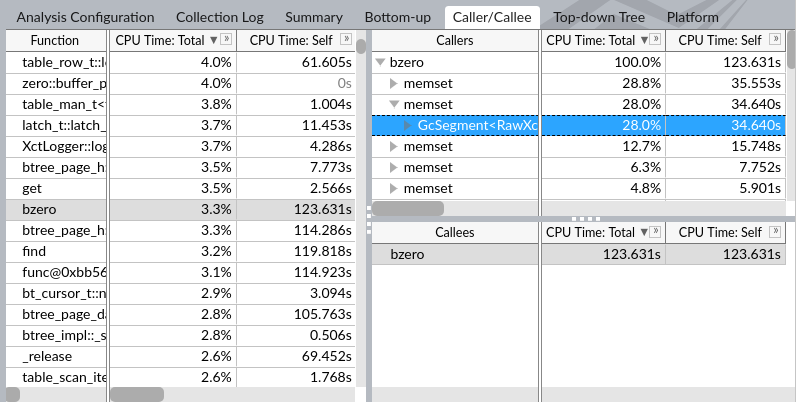
\includegraphics[width = \textwidth]{data/bzero.png}%
        }
        \vspace{.75em}
        \caption[The VTune™ Profiler uncovers unnecessary memory erasure]{The ``Caller/Callee'' tab of an \textit{Intel® VTune™ Profiler} analysis can be used to find code that consumes a significant amount of CPU time.}
        \label{fig:bzero}
    \end{figure}
\end{@empty}

    Finding \emph{small blocks of code} that take up an \emph{unexpectedly large amount of computing time} (or other resources) is probably the most common and basic application of software tracing and profiling.

    The screenshot in figure \ref{fig:bzero} shows part of the ``Caller/Callee'' tab of the \textit{Intel® VTune™ Profiler} analysis of the multithreaded execution of \textit{TPC-C} on \textit{Zero}. The DBS spends \SI{3.3}{\percent} (including benchmark code etc.) of CPU time in \lstinline|bzero|, which \emph{erases memory areas}. Such a call is a good candidate to find unnecessarily used CPU cycles, because such a call is not needed if e.g. the respective memory area is not reused without initialization.

\begin{@empty}
    \begin{code}[h!]
        \begin{lstlisting}[numbers = left, language = C++]
struct GcSegment {
    /* ... */
    void recycle() {
            owner = 0;
            allocated_objects = 0;
            ::memset(objects, 0, sizeof(T) * total_objects);
    }
    /* ... */
}
        \end{lstlisting}
        \caption[Source code with unnecessary memory erasure]{The member function \lstinline|GcSegment::recycle| does unnecessarily erase a memory area.}
        \label{lst:bzero}
    \end{code}
\end{@empty}

    This is the case for the caller \lstinline|GcSegment<RawXct>::recycle| which is responsible for \SI{28}{\percent} of the CPU time spent running \lstinline|bzero|. Listing \ref{lst:bzero} shows the implementation of this member function. As soon as an object of class \lstinline|GcSegment| is no longer needed, it is prepared for later reuse by overwriting all its member variables with zero. \lstinline|bzero| is called by \lstinline|memset| on line 7 because it is called to write zeros into a given memory area. But since it can be guaranteed that no part of the member variable \lstinline|objects| is accessed after reuse before it is reinitialized, this call is unnecessary and a waste of CPU time.

\begin{@empty}
    \pgfplotsset{%
        every axis/.append style = {
            xlabel = {$\text{Transaction throughput }\left[\si{1\per\minute}\right]$},
            xlabel near ticks,
            x label style = {font = \small},
            xticklabel style = {font = \scriptsize},
            xmode = normal,
            xmin = 0,
            scaled x ticks = false,
            xbar = .8pt,
            ymin = -0.75,
            ymax = 1.75,
            bar width = 1.5em,
            ytick style = {draw = none},
            ytick = {0, 1},
            yticklabels = {Optimized, Baseline},
            y tick label style = {align = center,
                                  font = \footnotesize},
            ylabel near ticks,
            y label style = {font = \small},
            xmajorgrids = true,
            width = \textwidth,
            height = .2\textheight
        }
    }

    \begin{figure}[ht!]
        \centering
        \begin{tikzpicture}
            \begin{axis}
                \addplot[draw = Cyan, fill = Cyan!50] coordinates
                {(889279.6, 0) (883277.13, 1)};
            \end{axis}
        \end{tikzpicture}
        \caption[Transaction throughput without unnecessary bzero calls]{Transaction throughput of the \nameref{subsec:random} page replacement algorithm before and after removing unnecessary calls to \lstinline|bzero| (memory erasure) for the \textit{TPC-C} benchmark on 100 warehouses}
        \label{fig:bzerothroughput}
    \end{figure}
\end{@empty}

    Figure \ref{fig:bzero} shows the transaction throughput of \textit{Zero} when running the \textit{TPC-C} Benchmarks before and after removing the mentioned call of \lstinline|bzero|. Both versions use the RANDOM page replacement algorithm and do not use the pointer swizzling technique from subsection \ref{subsec:looking_glass_swizzling}. After saving these $\SI{3.3}{\percent} \cdot \SI{28}{\percent} = \SI{0.924}{\percent}$ of CPU cycles a \SI{\approx 0.67}{\percent} higher transaction throughput can be achieved.

\section{Conclusion} \label{sec:looking_glass_outro}

    While the measurements from ``OLTP through the Looking Glass, and What We Found There'' were driven by the idea of \emph{omitting certain guarantees and features} provided by relational DBMSs, the measurements for section \ref{sec:looking_glass} had the goal of \emph{optimizing certain components} of a DBMS. Using the \emph{tracing} and \emph{profiling} tool \textit{Intel® VTune™ Profiler} it was shown that, depending on the workload, different DBMS components require the largest proportion of CPU cycles. When many small transactions are executed, the transaction manager becomes a bottleneck, but with a balanced workload such as \textit{TPC-C}, key comparisons in the B-tree consume most CPU time.

    These results suggest an optimization of the \emph{transaction manager}. Since most of the CPU time was spent on spinning a spinlock, the complete removal of such a global latch would be an enormous optimization, making this component much more scalable. Optimizations in the \emph{B-tree} are---as demonstrated here again---also always beneficial, especially when executing \textit{TPC-C}. Even though \textit{Zero} uses the well optimized Foster B-tree---many other approaches to optimize B+trees are known. Some of them are described by Goetz Graefe in his book ``Modern B-tree techniques'' \cite{Graefe:2011}.

    When executing \textit{TPC-C}, the \emph{buffer pool} used unexpectedly much CPU time, considering that (almost) all accessed DB pages were in memory during the whole measurement. Therefore, an optimization of the buffer pool like the \emph{pointer swizzling} technique proposed by Graefe et al. in \cite{Graefe:2014} looks promising. However, the performance evaluation of the technique in subsection \ref{subsec:looking_glass_swizzling} showed a decrease in transaction throughput when applied. However, subsection \ref{subsec:looking_glass_bzero} showed that \emph{removing a single line of code} can be enough to improve transaction throughput by \SI{\approx 0.67}{\percent}, which is remarkable given the ease of the change. But as long as the quality of the implementation of a DBMS is not extremely poor, not much unnecessary code should be found that requires a considerable amount of CPU cycles, so such success should not be easily repeatable.


    % glossary

    \sloppy

    \printbibliography                      % generates the bibliography
                [
                    env = bibliography,     % select the environment to control the layout of the bibliography
                    heading = bibliography, % select the heading of the bibliography, alternatives can be defined using \defbibheading
%                    title = Bibliography,  % select the title of the bibliography
%                    prenote = prenote,     % select a note to be printed directly after the heading of the bibliography defined by \defbibnote
%                    postnote = postnote,   % select a note to be printed directly after the list of references of the bibliography defined by \defbibnote
%                    filter = bibfilter     % select a filter as defined in \defbibfilter
                ]

\end{document}
